% \documentclass{article}
\documentclass[UTF8]{article}
% \usepackage{xeCJK}
\usepackage{ctex}
% if you need to pass options to natbib, use, e.g.:
%\PassOptionsToPackage{numbers, compress}{natbib}
% before loading nips_2017
%
% to avoid loading the natbib package, add option nonatbib:
% \usepackage[nonatbib]{nips_2017}

\usepackage[final]{nips_2017}

% to compile a camera-ready version, add the [final] option, e.g.:
% \usepackage[final]{nips_2017}

\usepackage[utf8]{inputenc} % allow utf-8 input
\usepackage[T1]{fontenc}    % use 8-bit T1 fonts
\DeclareRobustCommand\nobreakspace{\leavevmode\nobreak\ }
\usepackage{hyperref}       % hyperlinks
\usepackage{url}            % simple URL typesetting
\usepackage{booktabs}       % professional-quality tables
\usepackage{amsfonts}       % blackboard math symbols
\usepackage{nicefrac}       % compact symbols for 1/2, etc.
\usepackage{microtype}      % microtypography
\usepackage{bm}             % bold in math
\usepackage{graphicx}       % images
\usepackage{algorithm}      % algorithm
\usepackage[noend]{algpseudocode} % algorithm
\usepackage{caption}        % captionof
\usepackage{array}          % thick column hline
\usepackage{booktabs}       % table style
\usepackage{pbox}           % table line break
\usepackage{subcaption}     % multiple figures
\usepackage{listings}
\usepackage{xcolor}
\usepackage{tikz}
\usepackage{amsmath}
\definecolor{mygreen}{rgb}{0,0.6,0}
\definecolor{mygray}{rgb}{0.5,0.5,0.5}
\definecolor{mymauve}{rgb}{0.58,0,0.82}
\definecolor{codeBkg}{rgb}{0.85,0.85,0.85}

\lstset{
	backgroundcolor=\color{codeBkg},   % choose the background color; you must add \usepackage{color} or \usepackage{xcolor}; should come as last argument
	basicstyle=\footnotesize,        % the size of the fonts that are used for the code
	breakatwhitespace=false,         % sets if automatic breaks should only happen at whitespace
	breaklines=true,                 % sets automatic line breaking
	captionpos=b,                    % sets the caption-position to bottom
	commentstyle=\color{mygreen},    % comment style
	deletekeywords={...},            % if you want to delete keywords from the given language
	escapeinside={\%*}{*)},          % if you want to add LaTeX within your code
	extendedchars=true,              % lets you use non-ASCII characters; for 8-bits encodings only, does not work with UTF-8
	frame=no,	                   % adds a frame around the code
	keepspaces=true,                 % keeps spaces in text, useful for keeping indentation of code (possibly needs columns=flexible)
	keywordstyle=\color{blue},       % keyword style
	language=Octave,                 % the language of the code
	morekeywords={*,...},            % if you want to add more keywords to the set
	numbers=left,                    % where to put the line-numbers; possible values are (none, left, right)
	numbersep=5pt,                   % how far the line-numbers are from the code
	numberstyle=\tiny\color{mygray}, % the style that is used for the line-numbers
	rulecolor=\color{black},         % if not set, the frame-color may be changed on line-breaks within not-black text (e.g. comments (green here))
	showspaces=false,                % show spaces everywhere adding particular underscores; it overrides 'showstringspaces'
	showstringspaces=false,          % underline spaces within strings only
	showtabs=false,                  % show tabs within strings adding particular underscores
	stepnumber=1,                    % the step between two line-numbers. If it's 1, each line will be numbered
	stringstyle=\color{mymauve},     % string literal style
	tabsize=4,	                   % sets default tabsize to 2 spaces
	title=\lstname                  % show the filename of files included with \lstinputlisting; also try caption instead of title
}

\title{PyTorch从入门到精通}

\hypersetup{
    colorlinks = true,
}
\makeatletter
\def\BState{\State\hskip-\ALG@thistlm}
\makeatother
\floatname{algorithm}{Procedure}
\renewcommand{\algorithmicrequire}{\textbf{Input:}}
\renewcommand{\algorithmicensure}{\textbf{Output:}}

\newcolumntype{?}{!{\vrule width 3pt}}

\author{
  闫涛 \\
  %% examples of more authors
  %% \And
  %% Nicholas Frosst \\
  %% Affiliation \\
  %% Address \\
  %% \texttt{email} \\
  %% \AND
  %% Geoffrey E. Hinton \\
  科技有限公司\\
  北京 \\
  \texttt{\{yt7589\}@qq.com} \\
  %% Affiliation \\
  %% Address \\
  %% \texttt{email} \\
  %% \And
  %% Coauthor \\
  %% Affiliation \\
  %% Address \\
  %% \texttt{email} \\
  %% \And
  %% Coauthor \\
  %% Affiliation \\
  %% Address \\
  %% \texttt{email} \\
}
\date{Dec 2019}

% \usepackage{natbib}
% \usepackage{graphicx}

\begin{document}


\newpage
\maketitle
\begin{center}
\Large \textbf{第1章 张量} \quad 
\end{center}
\begin{abstract}
在本章中我们将讨论PyTorch的基础概念张量(Tensor),包括创建、基本属性、基本操作,同时会稍微涉及一下底层原理,是后续学习的基础。
\end{abstract}
\section{张量概述}
在PyTorch中,尤其是在深度学习应用中,几乎所有运算都是以张量(Tensor)作为输入、输出类型,因此掌握张量(Tensor)的使用,是非常重要的。对于张量的官方介绍大家可以参考\cite{pytorch-tensor-intro},简单说明见\cite{csdn-blog-my-tensor1}的博文。
\subsection{创建}
我们首先需要可以创建张量(Tensor),在PyTorch中有多种方式可以创建张量(Tensor),在这里我们对各种创建方式都会有所提及,但是会重点讲述在实际中最常用的方法。
创建张量(Tensor)程序如下所示:
\lstset{language=PYTHON, caption={创建张量(app.pytorch.book.chp001.chp001\_c001.py)}, label={tensor-create-tensor}}
\begin{lstlisting}
import numpy as np
import torch

class Chp001C001(object):
    def __init__(self):
        self.name = 'app.pytorch.book.chp001.Chp001C001'

    def run(self):
        t1 = torch.empty(5)
        t2 = torch.empty([5, 3]) # 创建5*3空张量,元素值为随机数
        t3 = torch.rand(2, 3) # 采用0~1的均匀分布随机数初始化二维张量
        t4 = torch.randn(2, 3) # 以均值为0,方差为1的正态分布初始化二维张量
        t5 = torch.tensor([1.0, 2.0, 3.0, 4.0, 5.0]) # 最常用方法
        t6 = torch.Tensor([1.0, 2.0, 3.0, 4.0, 5.0]) # 利用构造函数
        # 元素全为1的张量
        t7 = torch.ones(2, 3, dtype=torch.float32) 
        t7_1 = torch.ones_like(t2) # 生成5*3二维张量,元素全为1
        # 创建元素值全为0的张量
        t8 = torch.zeros(2, 3, dtype=torch.int)
        t8_1 = torch.zeros_like(t2)

        print('t1:{0}'.format(t1))
        print('t2:{0}'.format(t2))
        print('t3:{0}'.format(t3))
        print('t4:{0}'.format(t4))
        print('t5:{0}'.format(t5))
        print('t6:{0}'.format(t6))
        print('t7:{0}'.format(t7))
        print('t7_1:{0}'.format(t7_1))
        print('t8:{0}'.format(t8))
        print('t8_1:{0}'.format(t8_1))
\end{lstlisting}
运行结果如下所示:
\begin{figure}[H]
	\caption{创建张量(Tensor)运行结果}
	\label{f000001}
	\centering
	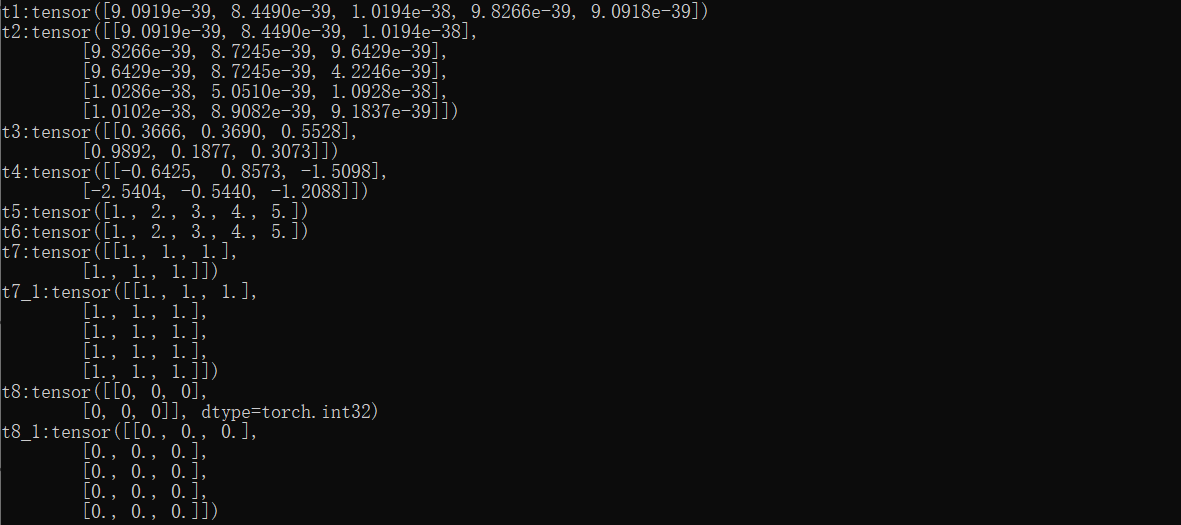
\includegraphics[width=15cm]{images/f000001}
\end{figure}
代码解析如下所示:
\begin{itemize}
\item 第9行:创建5个元素的一维张量,并且元素的值为对应内存位置的值,完全随机的值;
\item 第10行:创建5$\times$3的二维张量,元素的值为随机内容;
\item 第11行:创建2$\times$3的二维张量,元素的值由0$\sim$1之间的均匀分布的随机数进行初始化;
\item 第12行:创建2$\times$3的二维张量,元素的值由均值为0方差为1的正态分布的随机数进行初始化;
\item 第13行:由Python列表对象创建张量,这是我们最常使用的方法之一,在后面会详细讲解其用法;
\item 第14行:同样我们还可以用张量类的构造函数来创建,在实际中用的较少,了解即可;
\item 第16行:创建2$\times$3的二维张量,元素值全为1,并且设置数据类型为float32,在PyTorch中,缺省类型就是float32;
\item 第17行:创建与参数张量形状相同的张量,元素值全为1;
\item 第19行:创建2$\times$3的二维张量,元素值全为0,并且设置数据类型为int;
\item 第20行:创建与参数张量形状相同的张量,元素值全为;
\end{itemize}
我们在实际应用中,使用tensor方法来创建张量最常用,这个函数的使用方式为:
\lstset{language=PYTHON, caption={张量基本属性(app.pytorch.book.chp001.chp001\_c001.py)}, label={tensor-tensor-attribute}}
\begin{lstlisting}
    def test(self):
        t1 = torch.tensor([1.0, 2.0, 3.0])
        print('t1 dtype:{0}; device:{1}; layout:{2}'.format(t1.dtype, t1.device, t1.layout))
        t2 = torch.tensor([1.0, 2.0, 3.0], dtype=torch.float64, device=torch.device('cuda:0'))
        print(t2)
\end{lstlisting}
运行结果如下所示:
\begin{figure}[H]
	\caption{张量基本属性(Tensor)运行结果}
	\label{f000002}
	\centering
	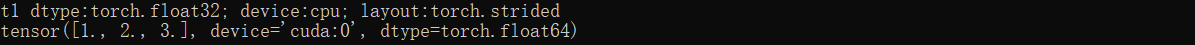
\includegraphics[width=15cm]{images/f000002}
\end{figure}
在上面的代码中,我们首先用缺省的方法创建张量t1,我们可以看到其缺省的dtype为float32,缺省创建在CPU上,缺省的内存布局为strided。接着我们创建张量t2,其类型为float64,并且创建在第一块GPU上。
\subsection{张量属性}
张量最重要的属性是其形状,其次是其轴,我们通过具体的代码来熟悉这些概念。
\lstset{language=PYTHON, caption={张量基本属性(app.pytorch.book.chp001.chp001\_c002.py)}, label={tensor-tensor-properties}}
\begin{lstlisting}
    def run(self):
        t1 = torch.tensor([
            [11.0, 12.0, 13.0, 14.0, 15.0],
            [21.0, 22.0, 23.0, 24.0, 25.0],
            [31.0, 32.0, 33.0, 34.0, 35.0]
        ])
        print('t1 size:{0}; shape:{1}; axis0:{2}'.format(t1.size(), t1.shape, t1.shape[0]))
        t2 = torch.tensor([
            [41.0, 42.0, 43.0, 44.0, 45.0]
        ])
        t3 = torch.cat((t1, t2), dim=0)
        print('t3 size:{0}\n{1}'.format(t3.shape, t3))
        t4 = torch.tensor([
            [101.0],
            [102.0],
            [103.0],
            [104.0]
        ])
        t5 = torch.cat((t3, t4), dim=1)
        print('t5 size:{0}\n{1}'.format(t5.shape, t5))
\end{lstlisting}
运行结果如下所示:
\begin{figure}[H]
	\caption{张量性质(Tensor)运行结果}
	\label{f000003}
	\centering
	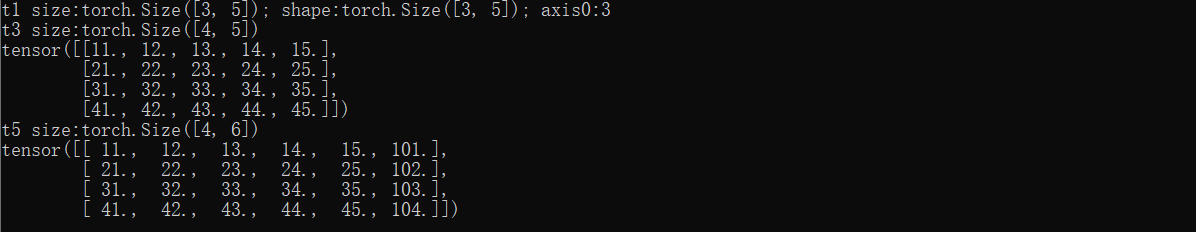
\includegraphics[width=15cm]{images/f000003}
\end{figure}
代码解析如下所示:
\begin{itemize}
\item 第2$\sim$6行:创建一个3$\times$5的二维张量t1;
\item 第7行:其形状可以由size()函数或shape属性得到,返回值为一个tuple,所以可以通过下标分别获取;
\item 第8$\sim$10行:声明一个1$\times$5的二维张量t2;
\item 第11行:将t2作为最后一行叠加到t1上,这里dim=0,表明叠加的轴是第0维;
\item 第12行:此时t3的形状为4$\times$5,最后一行为t2;
\item 第13$\sim$18行:生成一个4$\times$1的二维向量;
\item 第19行:将t4叠加到t3的后面,指定dim=1,表明在第1维上进行叠加;
\item 第20行:此时t5形状为4$\times$6,最后一列为t4;
\end{itemize}
\subsection{与numpy互操作}
在科学计算中,最常用的库是numpy,PyTorch可以视为是对numpy在GPU上的扩展。通常我们会需要将numpy的ndarray转换为张量,同时也需要将张量转换为ndarray,我们推荐大家使用的方法如下所示:
\lstset{language=PYTHON, caption={tensor和numpy互操作(app.pytorch.book.chp001.chp001\_c003.py)}, label={tensor-tensor-numpy}}
\begin{lstlisting}
    def run(self):
        v1 = np.array([
            [11.0, 12.0, 13.0, 14.0, 15.0],
            [21.0, 22.0, 23.0, 24.0, 25.0],
            [31.0, 32.0, 33.0, 34.0, 35.0]
        ], dtype=np.float32)
        t1 = torch.from_numpy(v1)
        print('t1:{0}'.format(t1))
        t2 = torch.tensor([101.0, 202.0, 303.0])
        v2 = t2.numpy()
        print('v2:{0}'.format(v2))
        v1[0][0] = 0.0
        v1[0][1] = 0.0
        print('修改后的t1:{0}'.format(t1))
        t2[0] = 0.0
        print('修改后的v2:{0}'.format(v2))
\end{lstlisting}
运行结果如下所示:
\begin{figure}[H]
	\caption{tensor和numpy互操作运行结果}
	\label{f000004}
	\centering
	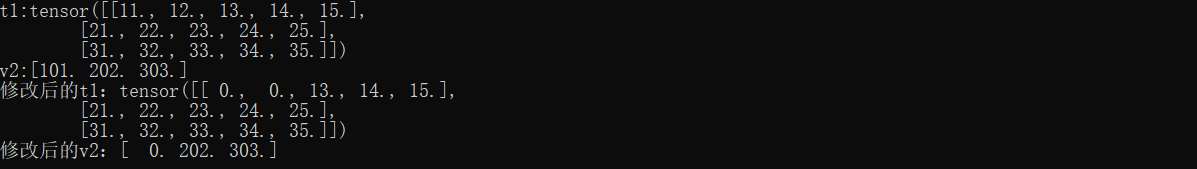
\includegraphics[width=15cm]{images/f000004}
\end{figure}
代码解读如下所示:
\begin{itemize}
\item 第2$\sim$6行:生成一个numpy的ndarray对象;
\item 第7行:将其通过torch.from\_numpy函数,将其转变为对应的tensor;
\item 第8行:由打印的内容来看,其与ndarray形状和内容相同;
\item 第9行:生成一个张量;
\item 第10行:通过numpy()函数,将其转变为numpy的ndarray;
\item 第11行:打印该ndarray;
\item 第12、13行:修改原始的ndarray中的值;
\item 第14行:我们在打印由v1转换的张量t1时,发现其值也已经进行了修改,这说明二者是共用内存的;
\item 第15行:我们修改原始张量t2中的值;
\item 第16行:打印由t2转换的数组v2时,其值也发生了改变,这说明二者是共用内存的;
\end{itemize}
这里需要说明的一点就是PyTorch中的tensor和numpy中的ndarray是共用内存的,所以二者之间的转换,由于无需拷贝元素,所以开销是非常小的。
\subsection{张量操作}
PyTorch中张量主要有四大类运算:Reshape、Elementwise Operation、Reduction、Access,下面我们分别来进行介绍。
\subsubsection{改变形状}
在深度学习当中,我们需要知道张量的形状,经常需要改变张量的形状,来满足各种算法要求,程序如下所示:
\lstset{language=PYTHON, caption={张量形状和变形(app.pytorch.book.chp001.chp001\_c004.py)}, label={tensor-tensor-reshape}}
\begin{lstlisting}
    def run(self):
        t1 = torch.tensor([
            [1.1, 1.2, 1.3],
            [2.1, 2.2, 2.3],
            [3.1, 3.2, 3.3],
            [4.1, 4.2, 4.3]
        ])
        print('t1.shape:{0}'.format(t1.shape))
        t2 = t1.reshape(2, 6)
        print('t2.shape:{0}\r\n{1}'.format(t2.shape, t2))
        t3 = t1.reshape(-1, 4)
        print('t3.shape:{0}\r\n{1}'.format(t3.shape, t3))
        print('元素个数:t1={0}; t2={1}'.format(t1.numel(), t2.numel()))
        t4 = t1.reshape(1, -1).squeeze()
        print('t4:{0}; {1}'.format(t4.shape, t4))
        t7 = torch.rand(28, 28)
        t8 = t7.flatten()
        print(t8.shape)
        t5 = t1.unsqueeze(1)
        print('t5:{0}; {1}'.format(t5.shape, t5))
        t6 = t5.squeeze(1)
        print('t6:{0}; {1}'.format(t6.shape, t6))
        img1 = torch.rand(28, 28)
        img2 = torch.rand(28, 28)
        img3 = torch.rand(28, 28)
        X_raw = torch.cat((img1, img2, img3), dim=0).reshape(3, 28, 28)
        print('X_raw:{0}'.format(X_raw.shape))
        X = X_raw.unsqueeze(1)
        print('X:{0}'.format(X.shape))
        a0 = X.flatten(start_dim=1)
        print('a0.shape:{0}'.format(a0.shape))
\end{lstlisting}
运行结果如下所示:
\begin{figure}[H]
	\caption{张量形状及变形}
	\label{f000005}
	\centering
	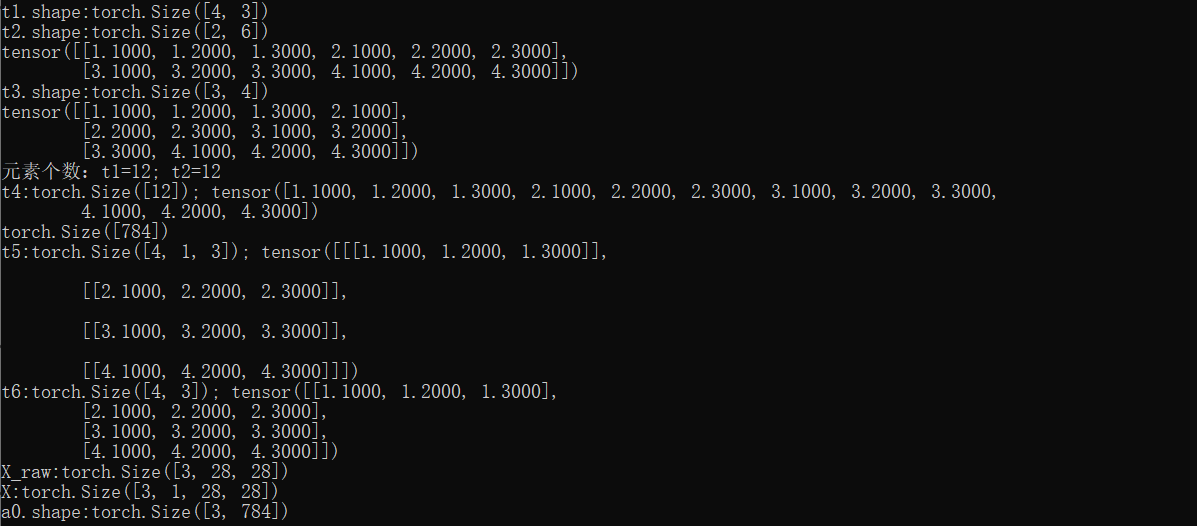
\includegraphics[width=15cm]{images/f000005}
\end{figure}
代码解读如下:
\begin{itemize}
\item 第2$\sim$7行:定义一个4$\times$3的二维张量;
\item 第8行:打印张量的原始形状;
\item 第9行:将张量的形状变为2$\times$6并赋给t2,注意这时t1的形状仍然为4$\times$3,t1和t2会共用内存,所以变形操作开销是非常小的;
\item 第10行:打印t2的内容,我们可以看到张量变形的算法原理:将原始张量展开为一维,然后重新进行分配;
\item 第11行:我们改变张量的形状,但是这时我们可以将一维指定为-1,PyTorch可以根据原始张量元素总数和其他维的数量推出此维数量;
\item 第12行:从打印的结果我们可以看出,PyTorch正确推出指定为-1的维的数量为3;
\item 第13行:可以通过numel()函数求出张量的元素数量;
\item 第14行:我们先将原始张量t1变为1$\times$12的张量,然后去掉第1维的1,变为[12]的张量,在后面我们将看到,这是一个常用的技巧;
\item 第15行:从打印结果可以看出,我们将原始的二维张量变为一维张量;
\item 第16$\sim$18行:我们声明一个28$\times$28的二维张量,通过调用torch.flatten函数,将其变为一维张量[784],其实这里实现的与第14行的方法相同;
\item 第19、20行:在第1维后增加一维,我们看到张量形状由4$\times$3,变为4$\times$1$\times$3;
\item 第21、22行:将上步加入的维度去掉,使形状由4$\times$1$\times$3重新变回4$\times$3;
\item 第23$\sim$25行:定义三个张量用来保存28$\times$28的图像数据;
\item 第26、27行:将三个图像数据按行叠加起来生成一个新张量,其形状为3$\times$28$\times$28;
\item 第28、29行:在第1维处加入一列,使其形状变为3$\times$1$\times$28$\times$28,这是图像处理应用中一种常见的格式,其中第一维代表迷你批次的索引号,第2维代表颜色,第3、4维为图像的宽度和高度;
\item 第30、31行:在实际神经网络中,需要将迷你批次中的图像,每一行一个图像的形式输入,即将张量的形状变为3$\times$784;
\end{itemize}
\subsubsection{元素操作}
我们经常需要对张量中的元素进行操作,可以分为四种情况:
\begin{enumerate}
\item 相同形状张量之间;
\item 张量与标量;
\item 不同形状张量之间;
\item 函数以张量作为参数;
\end{enumerate}
其中第一、二种情况,可以统一用Broadcast来进行理解。具体应用代码如下所示:
\lstset{language=PYTHON, caption={张量元素运算(app.pytorch.book.chp001.chp001\_c005.py)}, label={tensor-tensor-elementwise-operation}}
\begin{lstlisting}
    def run(self):
        t1 = torch.tensor([
            [1.1, 1.2, 1.3],
            [2.1, 2.2, 2.3]
        ])
        t2 = torch.tensor([
            [10.1, 11.0, 12.0],
            [20.0, 21.0, 22.0]
        ])
        print('操作符:\r\nt1+t2={0};\r\nt1-t2={1};\r\nt1*t2={2};'\
            '\r\nt1/t2={3}'\
            .format(t1+t2, t1-t2, t1*t2, t1/t2))
        print('函数:\r\nt1+t2={0};\r\nt1-t2={1};\r\nt1*t2={2};'\
            '\r\nt1/t2={3}'\
            .format(t1.add(t2), t1.sub(t2), t1.mul(t2), t1.div(t2)))
        print('张量加标量(操作符形式):\r\nt1+t2={0};\r\n'\
            't1-t2={1};\r\nt1*t2={2};\r\nt1/t2={3}'\
            .format(t1+2, t1-2, t1*2, t1/2))
        print('逻辑运算符:\r\nt1>1.2{0};\r\n'\
            't1<1.2{1};\r\nt1==1.1{2}'\
            .format(t1>1.2, t1<1.2, t1==1.1))
        t3 = torch.tensor([100.0, 200.0, 300.0])
        print('不同形状标量运算:\r\nt1+t3={0};\r\nt1-t3={1};\r\nt1*t3={2};'\
            '\r\nt1/t3={3}'\
            .format(t1+t3, t1-t3, t1*t3, t1/t3))
        print('以张量为参数函数:{0}'.format(self.fx(t1)))

    def fx(self, x):
        return x*100 + 8
\end{lstlisting}
运行结果如下所示:
\begin{figure}[H]
	\caption{张量元素运算运行结果}
	\label{f000006}
	\centering
	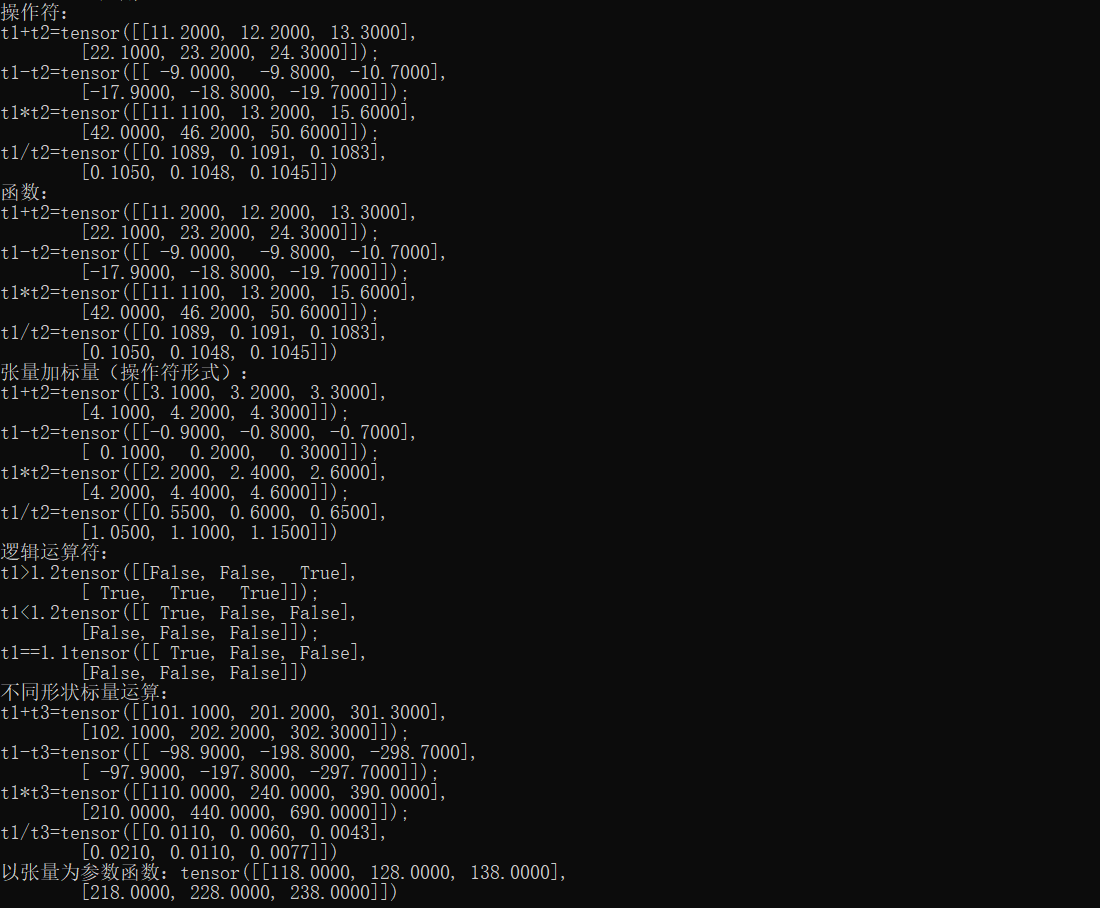
\includegraphics[width=15cm]{images/f000006}
\end{figure}
代码解读如下所示:
\begin{itemize}
\item 第2$\sim$5行:生成一个2$\times$3的张量;
\item 第6$\sim$9行:生成一个2$\times$3的张量t2;
\item 第10$\sim$12行:张量t1和t2之间加、减、乘、除运算,为对应位置元素进行相应的运算;
\item 第13$\sim$15行:除使用+、-、*、/运算外,还可以使用add、sub、mul、div函数,二者的效果相同;
\item 第16$\sim$18行:张量加一个标量,虽然我们可以简单的理解为拿标量对所有张量元素进行计算,但是实际上,PyTorch是进行了Broadcast操作,即在运算前将标量修改为:
\begin{equation}
2 \to \begin{bmatrix}
2.0 & 2.0 & 2.0 \\
2.0 & 2.0 & 2.0
\end{bmatrix}
\label{tensor-scala-broadcast-scala}
\end{equation}
这样就将问题转化为相同形状的张量之间的运算了。
\item 第19$\sim$21行:与张量与标量运算类似,也是先进行Broadcast操作,然对对应位置的元素进行逻辑运算,最后运算结果为True或False组成的同形状张量;
\item 第22行:我们定义一个与t1行形状相同的向量t3;
\item 第23$\sim$25行:PyTorch也首先进行Broadcast操作,将t3变为如下形式:
\begin{equation}
\begin{bmatrix}
100.0 & 200.0 & 300.0
\end{bmatrix} \to \begin{bmatrix}
100.0 & 200.0 & 300.0 \\
100.0 & 200.0 & 300.0
\end{bmatrix}
\label{tensor-scala-broadcast-tensor}
\end{equation}
这时就将问题转换为同形状张量之间的运算了。
\item 第26行:当函数参数为张量时,需要对张量每个元素应用该函数,结果为同形状张量;
\end{itemize}
\subsubsection{Reduction}
Reduction操作主要有求和、均值、方差,还有一个应用很广的函数argmax,用于多分类问题中找出正确的类别,代码如下所示:
\lstset{language=PYTHON, caption={张量Reduction(app.pytorch.book.chp001.chp001\_c006.py)}, label={tensor-tensor-reduction-operation}}
\begin{lstlisting}
    def run(self):
        t1 = torch.tensor([
            [1.0, 2.0, 3.0],
            [4.0, 5.0, 6.0]
        ])
        print('全部和:{0}; 行和:{1}; 列合:{2}'.format(t1.sum(), 
                    t1.sum(dim=1), t1.sum(dim=0)))
        print('均值:{0}; 行:{1}; 列:{2}'.format(t1.mean(), 
                    t1.mean(dim=1), t1.mean(dim=0)))
        print('方差:{0}; 行:{1}; 列:{2}'.format(t1.std(), 
                    t1.std(dim=1), t1.std(dim=0)))
        print('最大值:全部:{0}; 行:{1}; 列:{2}'.format(t1.max(), 
                    torch.max(t1, 1), torch.max(t1, 0)))
        t2 = torch.tensor([
            [0.1, 0.5, 0.4],
            [0.9, 0.05, 0.05]
        ])
        print('类别:{0}'.format(t2.argmax(dim=1)))
\end{lstlisting}
运行结果如下所示:
\begin{figure}[H]
	\caption{张量Reduction运算运行结果}
	\label{f000007}
	\centering
	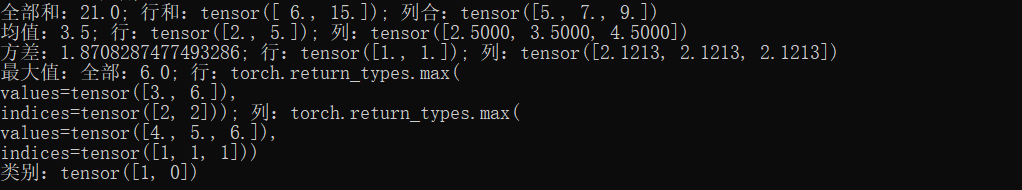
\includegraphics[width=15cm]{images/f000007}
\end{figure}
代码解读如下所示:
\begin{itemize}
\item 第2$\sim$5行:生成一个2$\times$3的二维张量t1;
\item 第6、7行:求出并打印全部元素的和,每行元素的和,每列元素的和;
\item 第8、9行:求出并打印全部元素的均值,每行元素的均值,每列元素的均值;
\item 第10、11行:求出并打印全部元素的方差,每行元素的方差,每列元素的方差;
\item 第12、13行:求出并打印全部元素的最大值,求出每行元素的最大值,返回结果values为每行的最大值,indices为每行最大元素所在的索引号。求出每列元素的最大值,返回结果values为每列的最大值,indices为每列最大元素所在的索引号;
\item 第12$\sim$17行:定义一个三分类问题,两个样本的输出层(采用softmax激活函数)输出值;
\item 第18行:用argmax求出每一行最大元素所在的索引号;
\end{itemize}
\subsubsection{索引和切片}
PyTorch中的张量既支持Python标准的切片方法,也支持一些特有的方法,如下所示:
\lstset{language=PYTHON, caption={张量索引和切片(app.pytorch.book.chp001.chp001\_c007.py)}, label={tensor-tensor-reduction-operation}}
\begin{lstlisting}
    def run(self):
        # cifar-10 16个样本为一个批次
        X = torch.rand(16, 3, 32, 32)
        # from zero start_idx(inclusive); end_idx(exclusive); step步长
        # 当为负数时由-1开始,表示是最后一个元素
        print('前两张图:{0}'.format(X[:2, :, :, :].shape))
        print('最后一张图:{0}'.format(X[-1:, :, :, :].shape))
        print('取偶数图片:{0}'.format(X[1::2, :, :, :].shape))
        print('选第1、8、9张图:{0}'.format(X.index_select(0, 
                    torch.tensor([0, 7, 8])).shape))
        print('取R和B两通道:{0}'.format(X.index_select(1, 
                    torch.tensor([0, 2])).shape))
        print('取每张图片8*8区域:{0}'.format( X.index_select(2, 
                    torch.arange(8)).index_select(3, 
                    torch.arange(6)).shape ))
        print('语法糖:第1张图:{0}; 颜色G通道:{1}'.format(
            X[0, ...].shape, X[:, 1, ...].shape)
        )
        mask = X.ge(0.5)
        print('大于0.5的元素:{0}'.format(
            torch.masked_select(X, mask))
        )
        t2 = torch.tensor([[3.0, 3.1, 3.2], [3.3, 3.4, 3.5]])
        print('按1维索引取值:{0}'.format(torch.take(t2, 
                    torch.tensor([0, 1, 5]))))
\end{lstlisting}
运行结果如下所示:
\begin{figure}[H]
	\caption{张量索引和切片运算运行结果}
	\label{f000008}
	\centering
	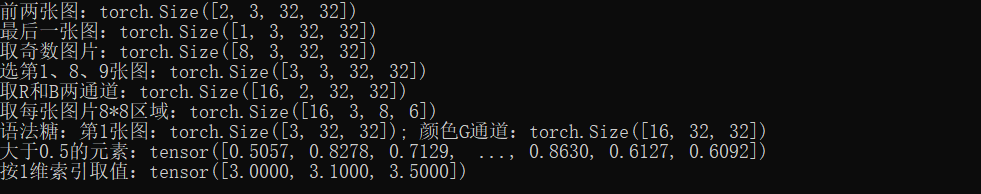
\includegraphics[width=15cm]{images/f000008}
\end{figure}
代码解读如下所示:
\begin{itemize}
\item 第3行:定义一个CIFAR-10数据集用于卷积神经网络输入的张量;
\item 第6行:X[:2, :, :, :]代表对第1维从索引号0开始,直到索引号2为止,但不包括索引号2,即表示批次中的第1、2个样本;
\item 第7行:代表从第1维最后一个元素开始,因此就是最后一张图片;
\item 第8行:对第1维从索引号为1开始,隔一个取一个,取偶数编号的图片;
\item 第9、10行:这里展示的是index\_select函数的用法,函数的第1个参数代表对哪一维进行操作,第二个参数用张量表示对该维哪些索引进行选取,这里第1个参数为零,代表对批次序号维进行操作,选索引号为0、7、8的元素,正好是第1、8、9张图片;
\item 第11、12行:index\_select的第1个参数为1,代表对颜色通道维进行操作,第2个参数为0、2则代表取RGB中的R和B通道数据;
\item 第13$\sim$15行:第一次index\_select调用中,第1个参数为2,代表从行数维取索引号在0$\sim$7之间的数据,第二次index\_select调用中,第1个参数为3,代表从列数维取索引号在0$\sim$5之间的数据,即取出所有图像左上角8$\times$6的子图像;
\item 第16$\sim$18行:这里展示的是一种语法糖,用...可以省略后面维度上取所有元素的:号;
\item 第19行:mask的元素为:如果对应位置X的元素大于0.5则其值为1,否则值为0,即其是由0或1组成的张量,形状与X相同,表示X的每个元素是否大于0.5;
\item 第20$\sim$22行:调用masked\_select函数,将X中值大于0.5的元素以1维张量形式返回;
\item 第23行:定义一个2$\times$3的二维张量;
\item 第24、25行:调用take方法,将张量t2,在指定索引号处的元素以1维张量形式返回;
\end{itemize}
\subsection{张量底层原理}
不知道大家有没有一个疑问,我们为什么不直接用Python中的列表,而是将其转换为张量在进行深度学习的运算呢?在本节中,我们简单介绍一下张量在内存中的表示,向大家展示,为什么张量的效率比Python的列表要高。\newline
假设我们定义如下的列表:
\lstset{language=PYTHON, caption={Python列表}, label={tensor-python-list}}
\begin{lstlisting}
t1 = [
	[1.0, 2.0, 3.0],
	[4.0, 5.0, 6.0]
]
\end{lstlisting}
其在内存中的存储如下所示:
\begin{figure}[H]
	\caption{Python列表内存存储}
	\label{f000009}
	\centering
	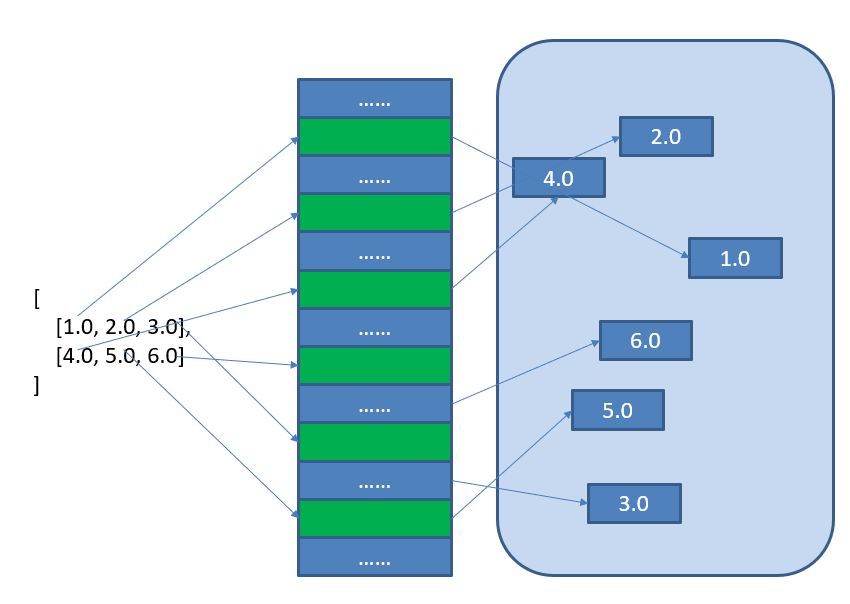
\includegraphics[height=6cm]{images/f000009}
\end{figure}
由上图可知,在Python中,数字也是以对象形式存储的。对于列表而言,每个元素对应于内存中的一个对象,对应着中间一列的内存地址,在该地址中,保存着实际值的地址,实际的数值保存在该地址中,所以对元素的获取,需要先找到元素对象地址,然后以该地址的内容作为内存地址,这样才能找到元素的具体值,需要两次寻址操作。\newline
我们再来看PyTorch下张量的内存存储:
\begin{figure}[H]
	\caption{PyTorch张量存储}
	\label{f000010}
	\centering
	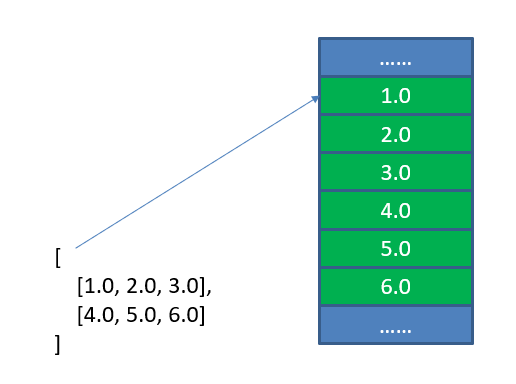
\includegraphics[height=6cm]{images/f000010}
\end{figure}
张量在内存中以连续的内存单元存储,而且直接保存数值,当我们获取某个元素时,假设该张量保存在以1000开头的内存地址中,我们要获取$t1[1][2]$元素,程序直接计算该元素的地址为:首地址 + idx1 * 阶2 + idx2 = 1000 + 1 * 3 + 2 = 1005,这个位置的元素值为6.0。由此可见,张量只需一步就可以获取到元素的值,而且改变张量形状后,获取元素时只需修改上面计算公式的参数即可,非常高效,而Python内置的列表对象,与此相比就要低效很多,所以我们在深度学习和其他科学计算任务中,很少使用Python内置的列表来表示数组,而是使用PyTorch的张量或numpy的ndarray来表示。\newline
我们在这里只是简单的介绍了一下张量存储的底层原理,如果想要了解更多内容,请大家参考\cite{deep-learning-with-pytorch}。
\subsection{总结}
在本章中,我们向大家详细介绍了PyTorch中的张量(Tensor),介绍了张量的创建、基本属性、与numpy的互操作和基本操作,其中基本操作中介绍了改变形状、元素操作、Reduction、索引和切片操作,并且以深度学习中常用的方式进行了介绍,最后我们简要介绍了PyTorch中张量在内存中的存储,介绍了为什么张量比Pyghon内置列表要高效的原因。\newline
在下一章中,我们将在此基础上,讲解自动微分技术,并且以张量和自动微分技术为基础,实现最简单的线性回归算法。



\newpage
\maketitle
\begin{center}
\Large \textbf{第2章 自动微分} \quad \textbf{}
\end{center}
\begin{abstract}
在本章中我们将自动微分技术,并且将直接使用自动微分技术,来解决线性回归问题。
\end{abstract}
\section{自动微分概述}
记得深度学习三巨头之一Yann LeCun曾经说过:“深度学习已死,可微编程永生”,就是说深度学习只是一种计算范式,而背后的可微分编程,具有更广阔的应用前景。在这里我们将探索PyTorch中的自动微分技术。
\subsection{数学原理}
在本节中,我们将讲述自动微分的数学原理,我们在这里将以深度学习的典型应用场景为例,来讲解自动微分的数学原理。
\subsubsection{函数以张量为参数}
PyTorch中的自动微分是基于Tensor的,以Tensor作为参数的函数,实际上是将Tensor中的每个元素应用该函数。只讲概念比较抽象,我们来看一个具体的例子。
我们定义$\boldsymbol{x} \in R^{5}$,定义如下函数:
\begin{equation}
y=f(\boldsymbol{x})=\begin{bmatrix}
f(x_{1}) \\
f(x_{2}) \\
f(x_{3}) \\
f(x_{4}) \\
f(x_{5})
\end{bmatrix}
\label{autodif-tensor-1}
\end{equation}
下面的程序我们以$x^{2}$为例:
\lstset{language=PYTHON, caption={求$x^{2}$函数以张量为参数}, label={autodiff-x2-param-tensor}}
\begin{lstlisting}
import torch
x = torch.tensor([1.0, 2.0, 3.0, 4.0, 5.0])
y = x ** 2
print(y)
# 输出结果为:tensor([ 1.,  4.,  9., 16., 25.])
\end{lstlisting}
在深度学习中,有三种最常见的情况:标量对向量的微分、向量对向量的微分、向量对矩阵的微分,其实还有张量对张量的微分,因为在实际中比较少见,所以这里就不再讨论了。
\subsubsection{标量对向量微分}
通常神经网络的代价函数会是一个标量,对于多分类问题,神经网络的输出为一个向量,这时就需要求标量对向量的微分。我们定义如下函数:
\begin{equation}
y = \sum_{i=1}^{5} x_{i}^{2}
\label{autodif-func-param-tensor-1}
\end{equation}
我们知道求微分可以采用解析法、数值法和自动微分法,由于这个问题比较简单,我们可以直接应用解析法:
\begin{equation}
\frac{ \partial{y} }{ \partial{x_{i}} } = 2x_{i}, \quad i=1,2,3,4,5
\label{autodif-func-param-tensor-1-gradient}
\end{equation}
我们定义标量对向量的微分为:
\begin{equation}
\frac{ \partial{y} }{ \partial{ \boldsymbol{x} } } = \begin{bmatrix}
\frac{ \partial{y} }{ \partial{x_{1}} } & \frac{ \partial{y} }{ \partial{x_{2}} } & \frac{ \partial{y} }{ \partial{x_{3}} } & \frac{ \partial{y} }{ \partial{x_{4}} } & \frac{ \partial{y} }{ \partial{x_{5}} }
\end{bmatrix} \in R^{1 \times n}, \quad \boldsymbol{x} \in R^{n}
\label{autodif-scalar-vector-gradient-def}
\end{equation}
我们可以通过PyTorch中的自动微分来完成这一任务:
\lstset{language=PYTHON, caption={标量对向量微分实现}, label={autodiff-scalar-vector-gradient-python}}
\begin{lstlisting}
x = torch.tensor([1.0, 2.0, 3.0, 4.0, 5.0], requires_grad=True, dtype=torch.float32)
y = torch.sum(x ** 2)
print(y.item()) # 打印计算值
y.backward() # 利用自动微分计算微分
print('shape:{0}; {1}'.format(x.grad.size(), x.grad)) # 打印y对x的微分值
# 打印结果:shape:torch.Size([5]); tensor([ 2.,  4.,  6.,  8., 10.])
\end{lstlisting}
代码解读如下:
\begin{itemize}
\item 第1行:我们在定义Tensor时,如果加入requires\_grad,表明我们需要求对其的微分;
\item 第2行:计算函数值,在实际应用中就是神经网络的前向传播过程;
\item 第4行:调用自动微分,就是实际应用中的神经网络的反向传播过程;
\end{itemize}
我们可以看到打印的结果与我们用解析法求出的内容一致。
\subsubsection{向量对向量微分}
实际上向量对向量微分叫做Jacobian矩阵,向量$\boldsymbol{y} \in R^{m}$对向量$\boldsymbol{x} \in R^{n}$的微分定义为:
\begin{equation}
\frac{ \partial{\boldsymbol{y}} }{ \partial{\boldsymbol{x}} } = \begin{bmatrix}
\frac{\partial{y_{1}}}{\partial{x_{1}}} & \frac{\partial{y_{1}}}{\partial{x_{2}}} & ... & \frac{\partial{y_{1}}}{\partial{x_{n}}} \\
\frac{\partial{y_{2}}}{\partial{x_{1}}} & \frac{\partial{y_{2}}}{\partial{x_{2}}} & ... & \frac{\partial{y_{2}}}{\partial{x_{n}}} \\
... & ... & ... & ... \\
\frac{\partial{y_{m}}}{\partial{x_{1}}} & \frac{\partial{y_{m}}}{\partial{x_{2}}} & ... & \frac{\partial{y_{m}}}{\partial{x_{n}}} \\
\end{bmatrix} \in R^{m \times n}
\label{autodif-vector-vector-gradient-def}
\end{equation}
我们假设有如下向量,例如是神经网络某层的输入向量:
\begin{equation}
\boldsymbol{z}^{l}=\begin{bmatrix}
1.0 \\
2.0 \\
3.0 \\
4.0 \\
5.0
\end{bmatrix}
\label{autodif-z-l}
\end{equation}
经过该层的激活函数(sigmoid函数)之后,得到本层的输出向量:
\begin{equation}
\boldsymbol{a}^{l}=\begin{bmatrix}
z_{1}^{2} \\
z_{2}^{2} \\
z_{1}^{3} \\
z_{1}^{4} \\
z_{1}^{5} \\
\end{bmatrix}
\label{autodif-a-l}
\end{equation}
因为本神经元的输入只会影响本神经元的输出,因此我们的$\boldsymbol{a}^{l}$如上所示。根据解析法可得其Jacobian矩阵为:
\begin{equation}
\frac{ \partial{\boldsymbol{a}^{l}} }{ \partial{\boldsymbol{z}^{l}} }=\begin{bmatrix}
\frac{ \partial{a}_{1}^{l} }{ \partial{z}_{1}^{l} } & 0 & 0 & 0 & 0 \\
0 & \frac{ \partial{a}_{2}^{l} }{ \partial{z}_{2}^{l} }  & 0 & 0 & 0 \\
0 & 0 & \frac{ \partial{a}_{3}^{l} }{ \partial{z}_{3}^{l} }  & 0 & 0 \\
0 & 0 & 0 & \frac{ \partial{a}_{3}^{l} }{ \partial{z}_{3}^{l} }  & 0 \\
0 & 0 & 0 & 0 & \frac{ \partial{a}_{3}^{l} }{ \partial{z}_{3}^{l} } 
\end{bmatrix}
\label{autodif-vector-vector-gradient-demo}
\end{equation}
其实际上只有对角线上有值,因此在PyTorch中,为了更高效的处理问题,我们通常不需要原始的Jacobian矩阵,而是将其乘以一个与$\boldsymbol{a}^{l}$同维且元素均为1的向量,得到的结果向量的元素为对角线上的元素。
\begin{equation}
\frac{ \partial{\boldsymbol{a}^{l}} }{ \partial{\boldsymbol{z}^{l}} } \cdot \begin{bmatrix}
1.0 \\
1.0 \\
1.0 \\
1.0 \\
1.0
\end{bmatrix}=\begin{bmatrix}
\frac{ \partial{a}_{1}^{l} }{ \partial{z}_{1}^{l} } & 0 & 0 & 0 & 0 \\
0 & \frac{ \partial{a}_{2}^{l} }{ \partial{z}_{2}^{l} }  & 0 & 0 & 0 \\
0 & 0 & \frac{ \partial{a}_{3}^{l} }{ \partial{z}_{3}^{l} }  & 0 & 0 \\
0 & 0 & 0 & \frac{ \partial{a}_{3}^{l} }{ \partial{z}_{3}^{l} }  & 0 \\
0 & 0 & 0 & 0 & \frac{ \partial{a}_{3}^{l} }{ \partial{z}_{3}^{l} } 
\end{bmatrix} \cdot \begin{bmatrix}
1.0 \\
1.0 \\
1.0 \\
1.0 \\
1.0
\end{bmatrix}= \cdot \begin{bmatrix}
\frac{ \partial{a}_{1}^{l} }{ \partial{z}_{1}^{l} } \\
\frac{ \partial{a}_{2}^{l} }{ \partial{z}_{2}^{l} } \\
\frac{ \partial{a}_{2}^{l} }{ \partial{z}_{3}^{l} } \\
\frac{ \partial{a}_{4}^{l} }{ \partial{z}_{4}^{l} } \\
\frac{ \partial{a}_{5}^{l} }{ \partial{z}_{5}^{l} } 
\end{bmatrix}
\label{autodif-vector-vector-gradient-simplify}
\end{equation}
在PyTorch中代码如下所示:
\lstset{language=PYTHON, caption={向量对向量微分实现}, label={autodiff-vector-vector-gradient-python}}
\begin{lstlisting}
x = torch.tensor([1.0, 2.0, 3.0, 4.0, 5.0], requires_grad=True)
y = x**2
y.backward(torch.ones_like(y))
print('y_x:{0}'.format(x.grad))
# 输出:y_x:tensor([ 2.,  4.,  6.,  8., 10.])
\end{lstlisting}
\subsubsection{向量对矩阵微分}
在深度学习中,经常会出现上一层的输入向量$\boldsymbol{z}^{l} \in R^{N_{l}}$对连接权值$W^{l} \in R^{N_{l} \times N_{l-1}}$的微分,公式为:
\begin{equation}
\boldsymbol{z}^{l}=W^{l} \cdot \boldsymbol{a}^{l-1} + \boldsymbol{b}^{l}
\label{autodif-neural-network-layer-formula}
\end{equation}
其中$\boldsymbol{a}^{l-1} \in R^{N_{l-1}}$,$\boldsymbol{b}^{l} \in R^{N_{l}}$。\newline
通过解析法,我们可以得到其微分公式为:
\begin{equation}
\frac{ \partial{ \boldsymbol{z}^{l} } }{ \partial{W^{l}} } = \begin{bmatrix}
a_{1}^{l-1} & a_{2}^{l-1} & ... & a_{l-1}^{l-1} \\
a_{1}^{l-1} & a_{2}^{l-1} & ... & a_{l-1}^{l-1} \\
... & ... & ... & ... \\
a_{1}^{l-1} & a_{2}^{l-1} & ... & a_{l-1}^{l-1} \\
\end{bmatrix} = \begin{bmatrix}
(\boldsymbol{a}^{l-1})^{T} \\
(\boldsymbol{a}^{l-1})^{T} \\
... \\
(\boldsymbol{a}^{l-1})^{T}
\end{bmatrix} \in R^{ N_{l} \times N_{l-1} }
\label{autodif-neural-network-layer-W-gradient}
\end{equation}
PyTorch代码如下所示:
\lstset{language=PYTHON, caption={向量对矩阵微分实现}, label={autodiff-vector-matrix-gradient-python}}
\begin{lstlisting}
a_l_1 = torch.tensor([1.0, 2.0, 3.0, 4.0, 5.0], requires_grad=True)
W_l = torch.tensor([
    [101.0, 102.0, 103.0, 104.0, 105.0],
    [201.0, 202.0, 203.0, 204.0, 205.0],
    [301.0, 302.0, 303.0, 304.0, 305.0]
], requires_grad=True)
b_l = torch.tensor([1001.0, 1002.0, 1003.0], requires_grad=True)
z_l = torch.matmul(W_l, a_l_1) + b_l
z_l.backward(torch.ones_like(z_l))
print('y_x:{0}'.format(W_l.grad))
''' 打印输出
y_x:tensor([[1., 2., 3., 4., 5.],
    [1., 2., 3., 4., 5.],
    [1., 2., 3., 4., 5.]])
'''
\end{lstlisting}
由上面程序的运行结果可以看出,上述程序的打印结果与理论分析的结果一致,证明我们的求法是正确的。\newline
有了这些知识之后,我们就可以利用这些知识,写出复杂的神经网络了,在本章中,我们将使用这些底层的技术,来解决简单的线性回归问题。但是我们在实际应用中,通常我们会用PyTorch包装的高阶API来实现,因此在“线性回归”章节,我们将采用PyTorch通常的方式来求解线性回归问题。线性回归的数学原理,也将在“线性回归”章节详细讲解。
\subsection{自动微分求解线性回归}
在这里我们只以一个简单的线性回归为例,分别采用numpy和PyTorch自动微分来求解。\newline
我们采用如下的程序生成一个数据集,如下所示:
\lstset{language=PYTHON, caption={生成线性回归数据集}, label={autodiff-linear-regression-dataset}}
\begin{lstlisting}
    def load_dataset(self):
        delta = np.random.randn(10)*0.07
        X = np.linspace(0, 1, 10)
        y = 2*X + delta
        plt.rcParams['font.sans-serif'] = ['SimHei']
        plt.rcParams['axes.unicode_minus'] = False
        plt.title('线性回归数据集')
        plt.scatter(X, y, s=18)
        plt.plot(X, 2*X, '-r')
        plt.show()
        return X, y
\end{lstlisting}
生成的图像如下所示:
\begin{figure}[H]
	\caption{线性回归数据集}
	\label{f000011}
	\centering
	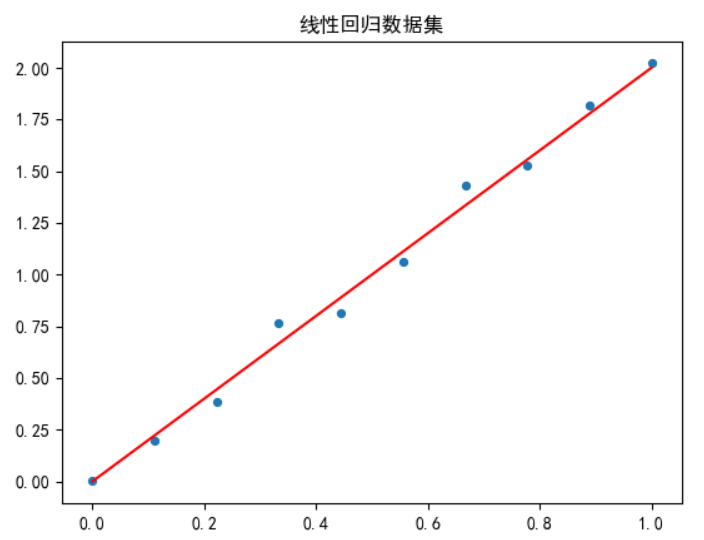
\includegraphics[height=10cm]{images/f000011}
\end{figure}
代码解读如下所示:
\begin{itemize}
\item 第2行:生成一个从标准正态分布$\mathcal(N)(0,1)$中取10个随机数,并将其缩小0.7倍;
\item 第3行:X为从0$\sim$1之间均匀取10个数;
\item 第4行:求出y值,为了增加问题的复杂性,我们这里加入了一个随机项,使其看起来不是一个完美的直线;
\item 第5、6行:设置绘图库的中文显示;
\item 第7行:设置图像标题;
\item 第8行:绘制散点图;
\item 第9行:绘制目标直线,我们线性回归的目标;
\end{itemize}
\subsubsection{使用numpy库}
下面我们用numpy来实现线性回归算法,在本章中我们只讲算法实现,在下一章“线性回归”中,我们将讲解线性回归的数学原理。代码如下所示:
\lstset{language=PYTHON, caption={numpy求解线性回归问题代码}, label={autodiff-linear-regression-numpy}}
\begin{lstlisting}
    def run(self):
        print('numpy求解线性回归')
        X, y = self.load_dataset()
        for epoch in range(100):
            for xi, yi in zip(X, y):
                y_hat = self.forward(xi)
                loss = self.loss(xi, yi)
                grad = self.gradient(xi, yi, y_hat)
                self.w -= self.learning_rate * grad
                print('{0}: loss:{1}; w:{2}'.format(epoch, loss, self.w))
        print('The End ^_^')
        self.draw_dataset(X, y, self.w)

    def forward(self, x):
        return x * self.w
    
    def loss(self, x, y):
        y_hat = self.forward(x)
        return (y_hat - y) * (y_hat - y)

    def gradient(self, x, y, y_hat):
        return 2.0 * x * (y_hat - y)


    def load_dataset(self):
        delta = np.random.randn(10)*0.06
        X = np.linspace(0, 1, 10)
        y = 2*X + delta
        return X, y

    def draw_dataset(self, X, y, w):
        plt.rcParams['font.sans-serif'] = ['SimHei']
        plt.rcParams['axes.unicode_minus'] = False
        plt.title('线性回归数据集')
        plt.scatter(X, y, s=18)
        plt.plot(X, 2*X, '-r')
        plt.plot(X, w*X, '-b')
        plt.show()
\end{lstlisting}
运行结果如下所示:
\begin{figure}[H]
	\caption{numpy求解线性回归问题运行结果}
	\label{f000012}
	\centering
	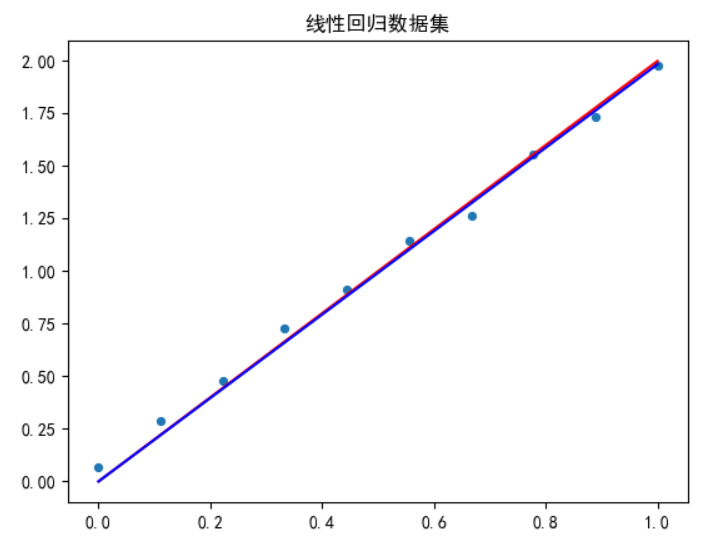
\includegraphics[height=10cm]{images/f000012}
\end{figure}
代码解读如下所示:
\begin{itemize}
\item 第3行:载入上面所讲的线性回归数据集;
\item 第4行:共进行100次迭代;
\item 第5行:对每个样本执行6$\sim$10行;
\item 第6行:调用forward方法(在后面讲解),求出该样本的输出值$\hat{y}$;
\item 第7行:以输入$x^{(i)}$和正确值$y^{(i)}$为参数,调用loss方法(在后面讲解),求出代价函数值;
\item 第8行:以输入$x^{(i)}$和正确值$y^{i}$和计算值$\hat{y}^{(i)}$为参数,调用gradient方法(在后面讲解),求出对参数的微分;
\item 第9行:由于我们要求的是代价函数的最小值,根据梯度下降算法调整参数:$w \leftarrow w - \alpha \cdot \nabla_{w} \mathcal{L}$;
\item 第10行:打印训练过程;
\item 第12行:绘制学习结果;
\item 第14、15行:定义前向传播方法forward,其计算公式为:$\hat{y}^{(i)} = w \cdot x^{(i)}$;
\item 第17$\sim$19行:定义代价函数计算方法,公式为:$\mathcal{L}(w) = (\hat{y}^{(i)} - y^{(i)})^{2}$;
\item 第21$\sim$22行:定义微分计算方法,公式推导如下:
\begin{equation}
\begin{aligned}
\frac{ \partial{ \mathcal{L}(w) } }{ \partial{w} } = \frac{ \partial{ (\hat{y}^{(i)} - y^{(i)})^{2} } }{ \partial{w} } \\
= \frac{ \partial{ (w \cdot x^{(i)} - y^{(i)})^{2} } }{ \partial{w} } \\
= \frac{ \partial{ (w \cdot x^{(i)} - y^{(i)})^{2} } } { \partial{ (w \cdot x^{(i)} - y^{(i)}) } } \cdot \frac{ \partial{ (w \cdot x^{(i)} - y^{(i)}) } }      { \partial{w} } \\
= 2 (w \cdot x^{(i)} - y^{(i)}) \cdot \frac{ \partial{(w \cdot x^{(i)} - y^{(i)})}}{\partial{w}} \\
= 2 x^{(i)}(w \cdot x^{(i)} - y^{(i)})
\end{aligned}
\label{autodiff-numpy-mse-gradient}
\end{equation}
\end{itemize}
我们来看最后我们学习得到的蓝色直线,与我们目标的红色直线非常接近,所以说明我们的算法可以很好的完成任务。
\subsubsection{使用PyTorch}
下面我们利用PyTorch的张量和自动微分技术来求解这个线性回归问题,注意我们在实际应用中,我们通常不会采用这种方式,而是采用集成度更高的PyTorch风格来解决这个问题,我们将在下一章中进行详细讲解。代码如下所示:
下面我们用numpy来实现线性回归算法,在本章中我们只讲算法实现,在下一章“线性回归”中,我们将讲解线性回归的数学原理。代码如下所示:
\lstset{language=PYTHON, caption={PyTorch求解线性回归问题代码}, label={autodiff-linear-regression-pytorch}}
\begin{lstlisting}
    def __init__(self):
        self.name = ''
        self.w = Variable(torch.tensor([1.0]), requires_grad=True)
        self.learning_rate = 0.01

    def run(self):
        X, y = self.load_dataset()
        for epoch in range(100):
            for xi, yi in zip(X, y):
                y_hat = self.forward(xi)
                loss = self.loss(xi, yi)
                loss.backward()
                #grad = self.gradient(x, y, y_hat)
                self.w.data -= self.learning_rate * self.w.grad.data
                self.w.grad.data.zero_()
                print('{0}: loss:{1}; w:{2}'.format(epoch, loss.data[0], self.w))
        self.draw_dataset(X.numpy(), y.numpy(), self.w.item())
        print('The End ^_^')

    def forward(self, x):
        return x * self.w
    
    def loss(self, x, y):
        y_hat = self.forward(x)
        return (y_hat - y) * (y_hat - y)

    def gradient(self, x, y, y_hat):
        return 2.0 * x * (y_hat - y)

    def load_dataset(self):
        delta = np.random.randn(10)*0.06
        X = np.linspace(0, 1, 10)
        y = 2*X + delta
        return torch.from_numpy(X), torch.from_numpy(y)

    def draw_dataset(self, X, y, w):
        plt.rcParams['font.sans-serif'] = ['SimHei']
        plt.rcParams['axes.unicode_minus'] = False
        plt.title('线性回归数据集')
        plt.scatter(X, y, s=18)
        plt.plot(X, 2*X, '-r')
        plt.plot(X, w*X, '-b')
        plt.show()
\end{lstlisting}
代码解读如下所示:
\begin{itemize}
\item 第3行:在构造函数中定义权值变量,在PyTorch中,需要学习的参数,统一定义为Variable;
\item 第4行:定义的学习率;
\item 第7行:载入我们前面介绍的数据集;
\item 第9行:对于每个样本执行10$\sim$16行;
\item 第10行:以输入样本$x^{(i)}$为参数调用forward方法(在后面讲解),求出计算值$\hat{y}^{(i)}$;
\item 第11行:以输入信号$x^{(i)}$和正确值$y^{(i)}$为参数,调用loss方法(在后面讲解)求代价函数值;
\item 第12行:调用PyTorch的反向传播方法,求对代价函数对网络参数的微分;
\item 第14行:由于我们要求的是代价函数的最小值,根据梯度下降算法调整参数:$w \leftarrow w - \alpha \cdot \nabla_{w} \mathcal{L}$;
\item 第15行:将参数的微分值清零,为下一个样本处理做准备;
\item 第16行:打印训练进度信息;
\item 第17行:打印训练后的结果图:

\begin{figure}[H]
	\caption{PyTorch求解线性回归问题运行结果}
	\label{f000013}
	\centering
	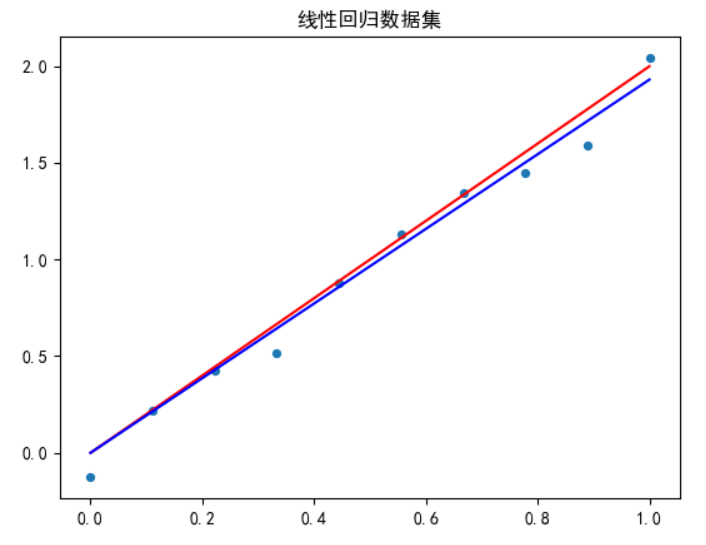
\includegraphics[height=10cm]{images/f000013}
\end{figure}
如上图所示,学习到的直线如蓝色直线所示,与真实的红色直线的差别并不大,证明我们算法是正确的,如果增加迭代次数,可以使学习到的直线更加逼近真实的直线。
\item 第20、21行:定义前向传播方法forward,计算值为:$\hat{y}^{(i)}=w \cdot x^{(i)}$;
\item 第23$\sim$25行:定义代价函数计算方法,公式为:$\mathcal{L}(w) = (\hat{y}^{(i)} - y^{(i)})^{2}$;
\item 第27、28行:定义微分计算方法,公式推导如下:
\begin{equation}
\begin{aligned}
\frac{ \partial{ \mathcal{L}(w) } }{ \partial{w} } = \frac{ \partial{ (\hat{y}^{(i)} - y^{(i)})^{2} } }{ \partial{w} } \\
= \frac{ \partial{ (w \cdot x^{(i)} - y^{(i)})^{2} } }{ \partial{w} } \\
= \frac{ \partial{ (w \cdot x^{(i)} - y^{(i)})^{2} } } { \partial{ (w \cdot x^{(i)} - y^{(i)}) } } \cdot \frac{ \partial{ (w \cdot x^{(i)} - y^{(i)}) } }      { \partial{w} } \\
= 2 (w \cdot x^{(i)} - y^{(i)}) \cdot \frac{ \partial{(w \cdot x^{(i)} - y^{(i)})}}{\partial{w}} \\
= 2 x^{(i)}(w \cdot x^{(i)} - y^{(i)})
\end{aligned}
\label{autodiff-pytorch-mse-gradient}
\end{equation}
\end{itemize}
\subsection{总结}
在本章中,我们结合深度学习的常用场景,讲解了怎样在PyTorch中使用自动微分技术来实现这些功能。接着我们分别展示了怎样使用numpy库实现线性回归问题求解,然后展示仅使用PyTorch中的张量和自动微分求解线性回归问题。有了这些基础知识,我们实际上可以构造出各种复杂的神经网络。但是实际应用中,我们通常采用PyTorch的高阶API来实现这些功能。在下一章中,我们将向大家讲解怎样用PyTorch的标准方法来求解线性回归问题,同时我们也将详细讲解线性回归的数学原理。

\newpage
\maketitle
\begin{center}
\Large \textbf{第3章 线性回归} \quad \textbf{}
\end{center}
\begin{abstract}
在本章中我们线性回归的数学原理,并利用PyTorch来求解线性回归问题。同时,我们会向大家进一步展示多项式回归,并讲解深度学习中的过拟合(over-fitting)问题。
\end{abstract}
\section{线性回归概述}
线性回归是最简单的一类机器学习算法,由于所要学习的函数是线性,而且是通过输入信号预测输出值,通常为一个标量,因此称之为线性回归。\newline
本节的应用实例,我们选择了一个初创公司估值模型。为了形象化理解这一问题,假设我们要拟合的数据由如下公式产生:$y = 2.0 \times x_{1} + 3.0 \times x_{2} + 2.6$。训练数据如下所示:
\begin{table}[H]
\centering
\caption{线性回归问题数据集}
\label{lrrn-dataset1}
\begin{tabular}{|c|c|c|} \hline
$x_{1}$ & $x_{2}$ & y \\ \hline 
0.54340494 & 0.2783694 & 4.521918 \\ \hline 
0.4245176  & 0.84477615  & 5.9833636 \\ \hline
0.00471886 & 0.12156912 & 2.974145 \\ \hline
0.67074907 & 0.82585275 & 6.419056 \\ \hline
0.13670659 & 0.5750933  & 4.598693 \\ \hline
0.89132196 & 0.20920213 & 5.01025 \\ \hline
0.18532822 & 0.10837689 & 3.2957869 \\ \hline
0.21969749 & 0.9786238 & 5.9752665 \\ \hline
0.8116832  & 0.17194101 & 4.739189 \\ \hline
0.81622475 & 0.27407375 & 5.054671 \\ \hline
\end{tabular}
\end{table}
\subsection{数学原理}
我们这里采用\cite{dl-tf-theano}书中的符号表示法,假设我们用$\boldsymbol{x}^{(i)}$来表示第$i$个训练样本,训练样本共有$m$个:$\{ \boldsymbol{x}^{(1)}, \boldsymbol{x}^{(2)}, ..., \boldsymbol{x}^{(m)} \}$,对于每个训练样本有n维,如下所示:
\begin{equation}
\boldsymbol{x}^{(i)} = \begin{bmatrix}
x_{1}^{(i)} \\
x_{2}^{(i)} \\
... \\
x_{n}^{(i)}
\end{bmatrix}
\label{lrrn-x-def}
\end{equation}
训练数据集的格式为:$(\boldsymbol{x}^{(i)}, y^{(i)})$,即为表\ref{lrrn-dataset1}中的一行。\newline
因为我们现在假设我们研究的是一个线性回归问题,即$\boldsymbol{x}^{(i)}$可由一个线性函数得到$y^{(i)}$,我们可以假设这个线性函数为如下形式:
\begin{equation}
y^{(i)} = \boldsymbol{w}^{T} \cdot \boldsymbol{x}^{(i)} + b, \quad \boldsymbol{w} \in R^{n}, \quad b \in R
\label{lrrn-linear-function-def}
\end{equation}
上式中$\boldsymbol{w}$和$b$为参数,是需要我们从数据集中学习出来的模型参数。\newline
上式用向量运算的形式表示,我们可以采用分量形式表示得更直观一些,以我们要研究的问题为例:
\begin{equation}
y^{(i)} = w_{1}x_{1}^{(i)} + w_{1}x_{1}^{(i)} + b, \quad \boldsymbol{w} \in R^{n}, \quad b \in R
\label{lrrn-linear-function-expand}
\end{equation}
为了衡量我们的模型好坏,对于单个样本,我们引入代价函数的概念:
\begin{equation}
l(\boldsymbol{\theta}) = \frac{1}{2} (\hat{y}^{(i)} - y^{(i)})^{2}
\label{lrrn-linear-regression-loss-i}
\end{equation}
我们将所有样本的代价函数定义为:
\begin{equation}
\mathcal{L}(\boldsymbol{\theta}) = \frac{1}{2} \sum_{i=1}^{m} (\hat{y}^{(i)} - y^{(i)})^{2}
\label{lrrn-linear-regression-loss}
\end{equation}
我们在今后的章节中,还会引入代价函数$\mathcal{J}(\boldsymbol{\theta})$,其定义为:$\mathcal{J}(\boldsymbol{\theta}) = \mathcal{J}(\boldsymbol{\theta}) + regualation$,即在式\ref{lrrn-linear-regression-loss}上再加入避免过拟合(Over-Fitting)的调整项后的结果。\newline
我们的目标是使总体代价函数越小越好,根据高等数学的相关知识,求一个函数的最小值,只需求该函数求对自变量的微分,令该微分为零,即可求出函数极值点时自动量的取值。在线性回归问题中,代价函数的自变量为$\boldsymbol{w}$和$b$,我们需要求对其的偏微分。求解这个问题有两种方法,一种是解析法,另一种是迭代法,下面我们分别来进行讲解。\newline
\subsubsection{迭代法求解}
我们首先来看第$i$个样本,我们先来求代价函数对$j$个参数的导数:
\begin{equation}
\begin{aligned}
\frac{ \partial{ l^{(i)}(\boldsymbol{\theta}) } }{ \partial{\theta _{j}} } = \frac{ \partial{ \frac{1}{2} (\hat{y}^{(i)} - y^{(i)})^{2} } }{ \partial{\theta _{j}} } \\
= \frac{1}{2} \frac{ \partial{ (\hat{y}^{(i)} - y^{(i)})^{2} } } { \partial{ (\hat{y}^{(i)} - y^{(i)}) } } \frac{{ \partial{ (\hat{y}^{(i)} - y^{(i)}) } }} { \partial{\theta _{j}} } \\
= (\hat{y}^{(i)} - y^{(i)}) \frac{ \partial{ (\theta _{0} + \theta _{1}x_{1}^{(i)} + \theta _{2}x_{2}^{(i)} + ... + \theta _{j}x_{j}^{(i)} + ... + \theta _{n}x_{n}^{(i)}  ) } }{ \partial{\theta _{j}} } \\
= (\hat{y}^{(i)} - y^{(i)})x_{j}^{(i)}
\end{aligned}
\label{lrrn-loss-gradient-samplei-thetaj}
\end{equation}
注意:在上式中$\theta _{0}$即为公式中的$b$。
而对一个批次中所有样本,微分定义为:
\begin{equation}
\frac{\partial{\mathcal{L}(\boldsymbol{\theta})}}{\theta _{j}} = \sum_{i=1}^{m} (\hat{y}^{(i)} - y^{(i)})x_{j}^{(i)}
\label{lrrn-loss-gradient-batch-theta-i}
\end{equation}
下面我们简单讲一下梯度下降算法,我们以求一个二次曲线极小值为例来讲解梯度下降算法。假设我们要求的二次曲线为:$f(x)=(x-1.5)^{2}$的图形为:
\begin{figure}[H]
	\caption{二次曲线梯度下降算法示意图}
	\label{f000014}
	\centering
	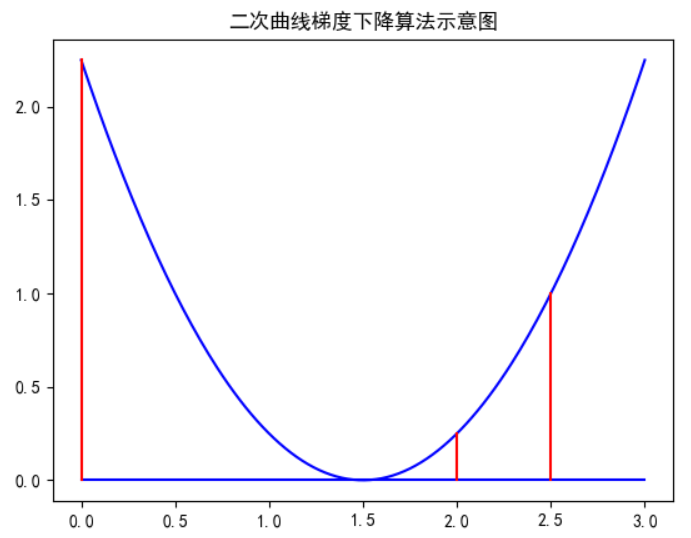
\includegraphics[height=10cm]{images/f000014}
\end{figure}
图形绘制代码见(resources/book/chp002/e1/chp002\_e1\_c002.py)我们求出该函数微分:$f'(x)=2(x-1.5)$,求当$x_{0}=2.5$时,$f(x_{0})=1$,微分值为$f'(x_{0})=2$,表明在该邻域内是单调增加的,想要求极小值,就要减少$x_{0}-\delta x$的值,而此时梯度的值为正值,就是需要减去梯度,例如,当$\delta x = 0.5$时,此时函数值为$f(x_{0} - \delta x)=f(2)=0.25$。但是我们也不能减小的太多,例如我们取$\delta x = 2.5$,此时$x_{0} - \delta x=0$,此时函数的值为$f(x_{0} - \delta x)=f(0)=2.25$,这时值反而会增大了,因此我们需要在微分前乘以一个小的正数,我们称之为学习率,在公式中用$\alpha$来表示。\newline
我们可以得到参数调整公式为:
\begin{equation}
\theta _{i} \leftarrow \theta _{i} - \alpha \frac{\partial{\mathcal{L}(\boldsymbol{\theta})}}{\theta _{j}}
\label{lrrn-parameter-update-formula}
\end{equation}


\subsubsection{解析法求解}
迭代法比较适合复杂的应用场景,对于简单的应用场景,例如我们现在所研究的线性回归算法而言,解析法是更高效的解决方案。所以,在这里向读者介绍一下解析法的推导过程,也帮助读者熟悉一下深度学习中所用到的数学知识。
首先介绍向量求导符号:
\begin{equation}
\nabla _{\boldsymbol{\theta}}\mathcal{L} = \frac{ \partial{\mathcal{L} }}{ \partial{\boldsymbol{\theta}} } = \begin{bmatrix}
\frac{ \partial{\mathcal{L} }}{ \partial{\theta _{0}} } & \frac{ \partial{\mathcal{L} }}{ \partial{\theta _{1}} } & \frac{ \partial{\mathcal{L} }}{ \partial{\theta _{2}} } & ... & \frac{ \partial{\mathcal{L} }}{ \partial{\theta _{n}} } \in R^{1 \times n+1}
\end{bmatrix}
\label{lrrn-scala-vector-gradient-def}
\end{equation}
则参数更新公式可以表示为:
\begin{equation}
\boldsymbol{\theta}^{T} \leftarrow \boldsymbol{\theta}^{T} - \alpha \nabla_{\boldsymbol{\theta}} \mathcal{L}
\label{lrrn-vector-parameter-update-formula}
\end{equation}
我们定义以矩阵为参数的函数$f:  R^{m \times n} \to R^{m \times n}$:
\begin{equation}
f(A) = \begin{bmatrix}
f(A_{1,1}) & f(A_{1,2}) & ... & f(A_{1,n}) \\
f(A_{2,1}) & f(A_{2,2}) & ... & f(A_{2,n}) \\
... \\
f(A_{m,1}) & f(A_{m,2}) & ... & f(A_{m,n})
\end{bmatrix}, A \in R^{m \times n}
\label{lrrn-function-matrix-parameter}
\end{equation}
我们可以定义对矩阵的微分为:
\begin{equation}
\nabla _{A}f(A) = \begin{bmatrix}
\frac{ \partial{f(A)} }{ \partial{A_{1,1}} } & \frac{ \partial{f(A)} }{ \partial{A_{1,2}} } & ... & \frac{ \partial{f(A)} }{ \partial{A_{1,n}} } \\
\frac{ \partial{f(A)} }{ \partial{A_{2,1}} } & \frac{ \partial{f(A)} }{ \partial{A_{2,2}} } & ... & \frac{ \partial{f(A)} }{ \partial{A_{2,n}} } \\
... \\
\frac{ \partial{f(A)} }{ \partial{A_{m,1}} } & \frac{ \partial{f(A)} }{ \partial{A_{m,2}} } & ... & \frac{ \partial{f(A)} }{ \partial{A_{m,n}} }
\end{bmatrix}
\label{lrrn-function-matrix-parameter-gradient}
\end{equation}
对于矩阵$A \in R^{m \times n}$的迹定义为:
\begin{equation}
tr A = \sum_{i=1}^{n} A_{i,i}
\label{lrrn-matrix-tr-def}
\end{equation}
矩阵的迹具有如下性质:
\begin{itemize}
\item $trAB = trBA$
\item $trABC = trCAB = trBCA$
\item $\nabla _{A} trAB = B^{T}$
\item $trA = trA^{T}$
\item 对$a \in R$,则$tr(a)=a$
\item $\nabla _{A} trABA^{T}C = CAB + C^{T}AB^{T}$
\end{itemize}
这些关于矩阵迹的性质将在后续的公式推导中用到,先在这里罗列出来,其实这些性质都是可以证明的,但是因为本书重点不是讲解数学知识,因此对证明过程感兴趣的读者可以查看其他相关资料。\newline
下面把$m$个$n$维的训练样本向量组成设计矩阵(Design Matrix):
\begin{equation}
X = \begin{bmatrix}
\Big( \boldsymbol{x}^{(1)} \Big)^{T} \\
\Big( \boldsymbol{x}^{(2)} \Big)^{T} \\
... \\
\Big( \boldsymbol{x}^{(m)} \Big)^{T}
\end{bmatrix}
\label{lrrn-design-matrix-def}
\end{equation}
则线性回归的公式可以表示为如下所示的形式:
\begin{equation}
\hat{\boldsymbol{y}} = X \cdot \boldsymbol{\theta} = \begin{bmatrix}
\Big( \boldsymbol{x}^{(1)} \Big)^{T} \\
\Big( \boldsymbol{x}^{(2)} \Big)^{T} \\
... \\
\Big( \boldsymbol{x}^{(m)} \Big)^{T}
\end{bmatrix} \cdot \boldsymbol{\theta} = \begin{bmatrix}
\Big( \boldsymbol{x}^{(1)} \Big)^{T} \cdot \boldsymbol{\theta} \\
\Big( \boldsymbol{x}^{(2)} \Big)^{T} \cdot \boldsymbol{\theta} \\
... \\
\Big( \boldsymbol{x}^{(m)} \Big)^{T} \cdot \boldsymbol{\theta}
\end{bmatrix} = \begin{bmatrix}
\hat{y}^{(1)} \\
\hat{y}^{(2)} \\
... \\
\hat{y}^{(m)} \\
\end{bmatrix}
\label{lrrn-linear-regression-formula-in-design-matrix}
\end{equation}
而正确结果可以表示为:
\begin{equation}
\boldsymbol{y} = \begin{bmatrix}
y^{(1)} \\
y^{(2)} \\
... \\
y^{(m)}
\end{bmatrix}
\label{lrrn-linear-regression-formula-target-truth}
\end{equation}
向量转置与向量的乘积为一个标量,公式为:
\begin{equation}
\boldsymbol{y}^{T} \boldsymbol{a} = \sum_{i=1}^{n} a_{i}^{2}
\label{lrrn-vector-t-vector-mul}
\end{equation}
我们根据这个公式推导出线性回归的代价函数公式:
\begin{equation}
\frac{1}{2}(\hat{\boldsymbol{y}} - \boldsymbol{y} )^{T} (\hat{\boldsymbol{y}} - \boldsymbol{y} ) = \frac{1}{2}\sum_{i=1}^{m} (\hat{y}^{(i)} - y^{(i)})^{2}
\label{lrrn-derive-loss-function}
\end{equation}
上式就是我们前面定义的线性回归代价函数公式。因此线性回归的公式可以变为:
\begin{equation}
\mathcal{L}(\boldsymbol{\theta}) = \frac{1}{2}(X \cdot \boldsymbol{\theta}- \boldsymbol{y} )^{T} (X \cdot \boldsymbol{\theta} - \boldsymbol{y} )
\label{lrrn-loss-function-in-vector}
\end{equation}
我们现在的任务是求代价函数的最小值,根据高等数学的知识可知,只需要对其求微分,使其值为零即可。
\begin{equation}
\begin{aligned}
\nabla _{\boldsymbol{\theta}} \mathcal{L}(\boldsymbol{\theta}) = \nabla _{\boldsymbol{\theta}} \frac{1}{2}(X \cdot \boldsymbol{\theta}- \boldsymbol{y} )^{T} (X \cdot \boldsymbol{\theta} - \boldsymbol{y} ) \quad (1) \\
= \frac{1}{2} \nabla _{\boldsymbol{\theta}} tr\Big( (X \cdot \boldsymbol{\theta}- \boldsymbol{y} )^{T} (X \cdot \boldsymbol{\theta} - \boldsymbol{y} ) \Big) (2) \\
= \frac{1}{2} \nabla _{\boldsymbol{\theta}} tr\Big( (\boldsymbol{\theta}^{T} X^{T} - \boldsymbol{y}^{T} ) (X \cdot \boldsymbol{\theta} - \boldsymbol{y} ) \Big) \quad (3) \\
= \frac{1}{2} \nabla _{\boldsymbol{\theta}} tr( \boldsymbol{\theta}^{T} X^{T}X \cdot \boldsymbol{\theta} -  \boldsymbol{\theta}^{T} X^{T}\boldsymbol{y} -  \boldsymbol{y}^{T}X \cdot \boldsymbol{\theta} + \boldsymbol{y}^{T} \boldsymbol{y}) \quad (4) \\
=\frac{1}{2} \nabla _{\boldsymbol{\theta}} \Big( tr(\boldsymbol{\theta}^{T} X^{T}X \cdot \boldsymbol{\theta}) - tr(\boldsymbol{\theta}^{T} X^{T}\boldsymbol{y}) -tr( \boldsymbol{y}^{T}X \cdot \boldsymbol{\theta}) \Big) \quad (5) \\
= \frac{1}{2} \nabla _{\boldsymbol{\theta}} \Big( tr(\boldsymbol{\theta}\boldsymbol{\theta}^{T} X^{T}X) - tr(\boldsymbol{\theta}^{T} X^{T}\boldsymbol{y}) -tr( \boldsymbol{y}^{T}X \cdot \boldsymbol{\theta}) \Big) \quad (6) \\
=\frac{1}{2}  \Big( \nabla _{\boldsymbol{\theta}}tr(\boldsymbol{\theta}\boldsymbol{\theta}^{T} X^{T}X)  - 2 \nabla _{\boldsymbol{\theta}} tr( \boldsymbol{y}^{T}X \boldsymbol{\theta}) \Big) \quad (7) \\
= \frac{1}{2} \Big( (X^{T}X\boldsymbol{\theta}I + X^{T}X\boldsymbol{\theta}I^{T})-2\nabla _{\boldsymbol{\theta}} tr( \boldsymbol{y}^{T}X \boldsymbol{\theta}) \Big) (8) \\
= \frac{1}{2} \Big( 2X^{T}X\boldsymbol{\theta} -2\nabla _{\boldsymbol{\theta}} tr( \boldsymbol{y}^{T}X \boldsymbol{\theta}) \Big) \quad (9) \\
= X^{T}X\boldsymbol{\theta} - \nabla _{\boldsymbol{\theta}} tr( \boldsymbol{y}^{T}X \boldsymbol{\theta}) \quad (10) \\
= X^{T}X\boldsymbol{\theta} - X^{T}\boldsymbol{y}=0
\end{aligned}
\label{lrrn-min-sq-mul}
\end{equation}
所以可以得到取得极小值时的参数为:
\begin{equation}
\boldsymbol{\theta} = (X^{T}X)^{-1}X^{T}\boldsymbol{y}
\label{lrrn-theta-star}
\end{equation}
上面的公式推导有些复杂,下面我们来做一下简单的解释:
\begin{itemize}
\item 第1行:直接使用式\ref{lrrn-loss-function-in-vector};
\item 第2行:由于代价函数是一个标量,而标量的迹等于标量,因此可以对其取迹运算而值不变;
\item 第3行:把整体的转置分解到各项,差的转置等于转置的差,另外用到转置的一个性质:$(AB)^{T}=B^{T}A^{T}$;
\item 第4行:将多项式乘积展开;
\item 第5行:由于我们是对$\boldsymbol{\theta}$求微分,最后一项$\boldsymbol{y}^{T}\boldsymbol{y}$为常量,因此微分为零被消去;另外迹的和差等于和差的迹;
\item 第6行:用到迹的性质:$trABC=trCAB$;
\item 第7行:根据迹的性质:$trA^{T}=trA$,可以合并后面两项;
\item 第8行:根据公式$\nabla _{A} trABA^{T}C = CAB + C^{T}AB^{T}$,我们设$A=\boldsymbol{\theta}$和$B=I$,其中$I$为单位阵,直接应用公式即可得到此式;
\item 第9行:单位阵乘以矩阵,结果还是该矩阵;
\item 第10行:将2与$\frac{1}{2}$约掉;
\item 第11行:根据公式$\nabla _{A} trAB = B^{T}$,直接应用公式即可得到本式;
\end{itemize}
上百就是用最小二乘法求出的参数向量的解析解的推导过程,但是要求$X^{T}X$可逆,在一般情况下,$X^{T}X$确实是可逆的。但是如果特征存在相互依赖的关系,此时$X^{T}X$就不可逆了,例如$x_{1} = 2x_{2}$,此时表明只有一个特征,而不是两个特征,因此就会出现不可逆情况。\newline
我们在实际应用中,很少用到解析法,所以在这里大家仅需要了解一下即可。
\subsection{线性回归求解}
我们首先通过程序生成前一节的数据集,然合利用PyTorch的Linear模型,来求解这个问题,求解完毕后,我们看一下求出的参数是否与真实参数吻合,同时给出一个例子,由模型进行预测,看预测的结果是否正确。\newline
我们先来看模型的定义:
\lstset{language=PYTHON, caption={线性模型定义(resources/book/chp002/e1/linear\_regression\_model.py)}, label={lrrn-module-def}}
\begin{lstlisting}
class LinearRegressionModel(torch.nn.Module):
    def __init__(self, in_features=1, out_features=1):
        super(LinearRegressionModel, self).__init__()
        self.linear = torch.nn.Linear(in_features=in_features, 
                    out_features=out_features, bias=True)

    def get_weights(self):
        return self.linear.weight
    
    def get_biases(self):
        return self.linear.bias

    def forward(self, x):
        return self.linear(x)
\end{lstlisting}
代码解读如下:
\begin{itemize}
\item 第1行:定义LinearRegressionModel类,并继承torch.nn.Module类;
\item 第4、5行:初始化线性模型,指定输入信号维度in\_features,输出信号维度out\_features,指定采用偏置值,即公式$\hat{y}^{(i)}=\boldsymbol{w}^{T} \cdot \boldsymbol{x}^{(i)} + b$中的$b$不为零;
\item 第7、8行:获取模型的权值,其值为张量;
\item 第10、11行:获取模型的偏置值,其值为张量;
\item 第13、14行:定义前向传播算法,在PyTorch中只需要定义前向传播算法,反向传输通过上一章的自动微分技术自动求出;
\end{itemize}
接下来我们来看怎样使用这个类:
\lstset{language=PYTHON, caption={线性回归示例(resources/book/chp002/e1/linear\_regression\_app.py)}, label={lrrn-lrrn-app}}
\begin{lstlisting}
class LinearRegressionApp(object):
    def __init__(self):
        self.name = ''
        
    def load_dataset(self):
        np.random.seed(100)
        X0 = np.random.rand(10, 2)
        X = np.array(X0, dtype=np.float32)
        w = np.array([2.0, 3.0], dtype=np.float32)
        b = 2.6
        y = np.matmul(X, w) + b
        y = y.reshape(10, 1)
        print('X:{0}; \r\ny:{1}'.format(X, y))
        return Variable(torch.from_numpy(X)), \
                    Variable(torch.from_numpy(y))

    def run(self):
        X_train, y_train = self.load_dataset()
        model = LinearRegressionModel(dim_in=2, dim_out=1)
        criterion = torch.nn.MSELoss(size_average=False)
        optimizer = torch.optim.SGD(model.parameters(), lr=0.01)
        #optimizer = torch.optim.Adam(model.parameters(), lr=0.01)
        for epoch in range(1000):
            y_hat = model(X_train)
            loss = criterion(y_hat, y_train)
            if epoch % 50 == 0:
                print('{0}: {1}'.format(epoch, loss.data.item()))
            optimizer.zero_grad()
            loss.backward()
            optimizer.step()
        w = model.get_weights().data
        bias = model.get_biases().data
        print('w:{0}; bias:{1}'.format(w, bias))
        

        x1 = Variable(torch.tensor([[4.0, 5.0]]))
        y1_hat = model.forward(x1).data[0][0]
        print('y={0}'.format(y1_hat))
\end{lstlisting}
代码解读如下所示:
\begin{itemize}
\item 第5行:定义生成数据集函数,生成表\ref{lrrn-dataset1}所示数据;
\item 第6行:让numpy每次生成的随机数相同,便于进行程序调试;
\item 第7行:从0$\sim$1的均匀分布中采样随机数,生成共有10个样本组成,每个样本为2维向量的ndarray;
\item 第8行:将数据类型由np.float64变为np.float32;
\item 第9行:设置权值参数的真值;
\item 第10行:设置偏置值的真值;
\item 第11行:根据公式:$\boldsymbol{y}=X \cdot \boldsymbol{w} + b$,因为$X \in R^{10 \times 2}$,$\boldsymbol{w} \in R^{2 \times 1}$,$b \in R$,所以$\boldsymbol{y} \in R^{10}$;
\item 第12行:将真值的维度由$R^{10}$变为$R^{10 \times 1}$;
\item 第14、15行:将$X$和$y$转换为PyTorch的变量类型并返回;
\item 第18行:载入数据集;
\item 第19行:生成线性回归模型对象,设置输入信号维度为2,输出信号维度为1;
\item 第20行:设置代价函数为MSE,即$\mathcal{L}=\sum_{i=1}^{m} (\hat{y}^{(i)} - y^{(i)})^{2}$;
\item 第21行:指定优化器为随机梯度下降算法;
\item 第23行:循环执行23$\sim$30行1000次;
\item 第24行:通过前向传播求出$\hat{Y}^{(i)}$;
\item 第25行:求出代价函数值;
\item 第26、27行:每隔50遍打印一次训练进展;
\item 第28行:清空网络参数的微分值;
\item 第29行:调用反向传播方法,利用PyTorch自动微分技术求出各参数的微分;
\item 第30行:利用优化器更新参数值;
\item 第31行:训练完成之后,取出模型的权值参数$\boldsymbol{w}$;
\item 第32行:取出偏置值参数$b$;
\item 第33行:打印权值和偏置值;
\item 第36行:生成一个测试用新的输入信号;
\item 第37行:利用前向传播求出网络的输出值;
\item 第38行:打印出该输出值;
\end{itemize}
程序运行结果如下所示:
\begin{figure}[H]
	\caption{线性回归运行结果}
	\label{f000015}
	\centering
	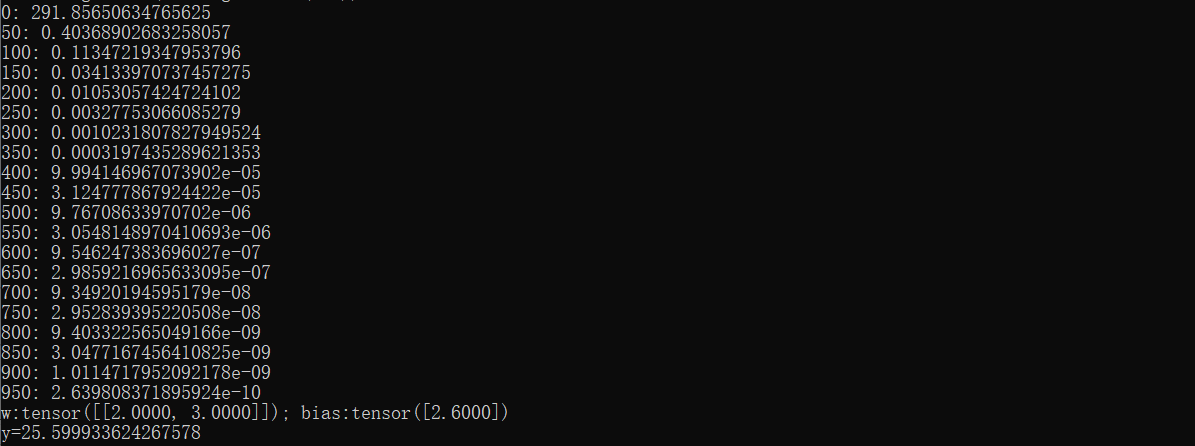
\includegraphics[width=15cm]{images/f000015}
\end{figure}
由运行结果可以看出,我们模型成功学出了所有的权值和偏置值,也可以预测新的样本值,证明我们线性回归应用是正确的。
\subsection{多项式回归}
在前面的章节的学习中,我们知道,线性回归实际上拟合的直线,而实际应用中,如果不是直线,如果是曲线的话要怎么处理呢?这个问题有两种处理思路:第一种是将其划分为足够多的段,而每段都可以用直线来近似,这样就将问题转化为多个线性回归的问题,就可以用我们前面章节介绍的技术来处理;第二种方法就是本节将介绍的多项式回归。在讲解具体的多项式回归算法之前,我们先来研究一下为什么多项式回归可以拟合任意的曲线。\newline
我们知道在高等数学中利用泰勒公式,可以将任意函数表示为多项式形式:
\begin{equation}
\begin{aligned}
f(x)=f(x_{0}) + f'(x_{0})(x-x_{0}) + \frac{f''(x_{0})}{2!}(x-x_{0})^{2} + \\
\frac{f^{(3)}(x_{0})}{3!}(x-x_{0})^{3} + ... + \frac{f^{(n)}(x_{0})}{n!}(x-x_{0})^{n} + ... \\
=\sum_{n=0}^{\infty} \frac{f^{(n)}(x_{0})}{n!} (x-x_{0})^{n}
\end{aligned}
\label{lrrn-taylor-formula}
\end{equation}
如果将$x_{0}=0$,上式就变为泰勒级数:
\begin{equation}
\begin{aligned}
f(x)=f(0) + f'(0)x + \frac{f''(0)}{2!}x^{2} + \\
\frac{f^{(3)}(0)}{3!}x^{3} + ... + \frac{f^{(n)}(0)}{n!}x^{n} + ... \\
=\sum_{n=0}^{\infty} \frac{f^{(n)}(0)}{n!} x^{n}
\end{aligned}
\label{lrrn-taylor-formula-x00}
\end{equation}
这就是我们可以使用多项式回归来拟合任意函数的理论依据,你要所拟合的函数无限可微,我们就可以以任意精度来拟合的这个函数。\newline
下面我们来看我们要拟合的曲线:
\lstset{language=PYTHON, caption={多项式回归示例(resources/book/chp002/e2/polynomial\_regression\_app.py)}, label={lrrn-polynomial-regress-target-function}}
\begin{lstlisting}
    def draw_curve(self):
        x = np.linspace(-1.5, 1.5, 1000)
        y = self.target_func(x)
        plt.rcParams['font.sans-serif'] = ['SimHei']
        plt.rcParams['axes.unicode_minus'] = False
        plt.title('二次曲线梯度下降算法示意图')
        plt.plot(x, y, '-b')
        plt.show()

    def target_func(self, x):
        return (x + 0.5)*(8.0*x - 1.0)
\end{lstlisting}
由于程序比较简单,我们就不讲解代码本身了,其定义的图形如下所示:
\begin{figure}[H]
	\caption{多项式回归目标曲线图}
	\label{f000016}
	\centering
	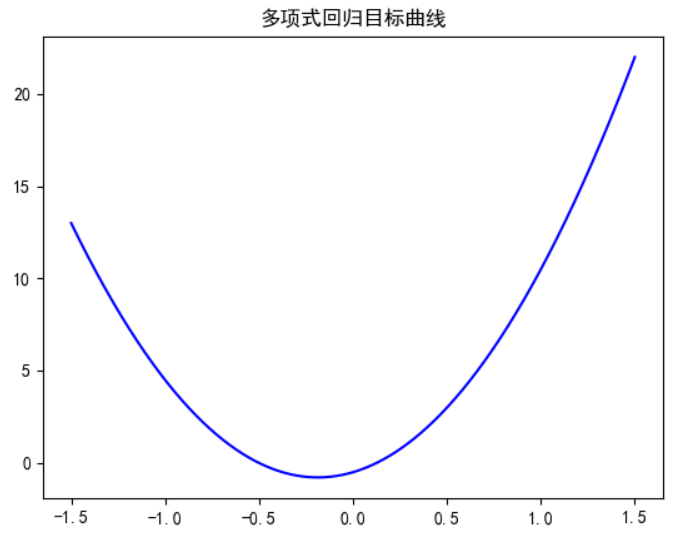
\includegraphics[height=10cm]{images/f000016}
\end{figure}
代码如下所示:
\lstset{language=PYTHON, caption={多项式回归示例(resources/book/chp002/e2/polynomial\_regression\_app.py)}, label={lrrn-polynomial-regression-app}}
\begin{lstlisting}
class PolynomialRegressionApp(object):
    def __init__(self):
        self.name = ''
        self.low_limit = -0.5
        self.high_limit = 0.5
        plt.rcParams['font.sans-serif'] = ['SimHei']
        plt.rcParams['axes.unicode_minus'] = False
        plt.title('多项式回归目标曲线')

    def run(self):
        rank = 9
        X_train, y_train = self.load_dataset(rank=rank)
        model = PolynomialRegressionModel(in_features=rank, out_features=1)
        criterion = torch.nn.MSELoss(size_average=False)
        optimizer = torch.optim.SGD(model.parameters(), lr=0.01)
        #optimizer = torch.optim.Adam(model.parameters(), lr=0.01)
        for epoch in range(8000):
            y_hat = model(X_train)
            loss = criterion(y_hat, y_train)
            if epoch % 50 == 0:
                print('{0}: {1}'.format(epoch, loss.data.item()))
            optimizer.zero_grad()
            loss.backward()
            optimizer.step()
        w = model.get_weights().data
        bias = model.get_biases().data
        print('w:{0}; bias:{1}'.format(w, bias))
        # 绘制学习的曲线
        test_data_x, test_np_x = self.generate_test_data(rank)
        test_input_x = Variable(torch.tensor([test_np_x]))
        test_y_hat = model.forward(test_input_x) 
        y_raw = test_y_hat.detach().numpy()
        y_hat = y_raw.reshape(y_raw.shape[1])
        plt.plot(test_data_x, y_hat, '-r')
        # 绘制数据散点图
        data_x = X_train[:, :1].flatten()
        data_y = self.target_func(data_x)
        plt.scatter(data_x, data_y)
        plt.show()

    def generate_test_data(self, rank):
        raw_data = np.linspace(self.low_limit, 
                    self.high_limit, 100)
        Xt1 = raw_data.reshape(raw_data.shape[0], 1)
        Xt2 = Xt1 * Xt1
        Xt3 = Xt2 * Xt1
        Xt4 = Xt3 * Xt1
        Xt5 = Xt4 * Xt1
        Xt6 = Xt5 * Xt1
        Xt7 = Xt6 * Xt1
        Xt8 = Xt7 * Xt1
        Xt9 = Xt8 * Xt1
        if 1 == rank:
            Xt = Xt1
        elif 2 == rank:
            Xt = np.hstack((Xt1, Xt2))
        else:
            Xt = np.hstack((Xt1, Xt2, Xt3, Xt4, Xt5, 
                        Xt6, Xt7, Xt8, Xt9))
        return raw_data, np.array(Xt, dtype=np.float32)
        
    def load_dataset(self, rank=1):
        np.random.seed(100)
        X1 = np.random.rand(10, 1) * (self.high_limit - \
                    self.low_limit) - (self.high_limit - \
                    self.low_limit) / 2.0
        X2 = X1 * X1
        X3 = X2 * X1
        X4 = X3 * X1
        X5 = X4 * X1
        X6 = X5 * X1
        X7 = X6 * X1
        X8 = X7 * X1
        X9 = X8 * X1
        if 1 == rank:
            X_raw = X1
        elif 2 == rank:
            X_raw = np.hstack((X1, X2)) 
        else:
            X_raw = np.hstack((X1, X2, X3, X4, X5, 
                        X6, X7, X8, X9))    
        X = np.array(X_raw, dtype=np.float32)
        b = 0.0
        y0 = self.target_func(X1)
        y = np.array(y0, dtype=np.float32)
        return Variable(torch.from_numpy(X)), \
                    Variable(torch.from_numpy(y))
\end{lstlisting}
代码解读如下所示:
\begin{itemize}
\item 第4、5行:规定数据集的下限和上限;
\item 第6$\sim$8行:设置matplotlib库可以显示中文和负号;
\item 第11行:设置多项式回归的最高项数,我们试验了1、2、9次方;
\item 第12行:载入数据集(方法将在后面讲解);
\item 第13行:创建多项式回归模型,对于$rank=1$时,$in_features=1$,$rank=2$时$in_features=2$,当$rank=9$时$in_features=9$;
\item 第14行:定义平方误差函数为代价函数;
\item 第15行:采用随机梯度下降算法作为优化方法;
\item 第17行:循环执行18$\sim$24行代码8000次;
\item 第18行:调用模型的forward方法求出网络输出值$\hat{Y}$;
\item 第19行:计算代价函数值;
\item 第20、21行:每隔50次迭代打印一次训练进度;
\item 第22行:清空网络参数的微分值;
\item 第23行:调用PyTorch自动微分反向传播算法网络参数微分;
\item 第24行:调用优化器根据参数微分更新参数值;
\item 第25行:获取训练好模型的权值参数$\boldsymbol{w}$;
\item 第26行:获取训练好模型的偏置值$b$;
\item 第27行:打印权值和偏置值;
\item 第29行:调用generate\_test\_data方法(将在后面介绍)生成原始的数据和按照多项式最高阶人工生成的数据;
\item 第30行:将阶数对应的数据转化为PyTorch的张量;
\item 第31行:调用模型forward方法求出网络输出值;
\item 第32、33行:取出结果张量将基转换为numpy数据且将形状变为$R^{m}$;
\item 第34行:绘制学习出的曲线;
\item 第36行:取出训练数据集第一列即一次项对应的数据;
\item 第37行:调用目标函数求出正确值;
\item 第38行:将训练数据集以散点图形式绘制出来;
\end{itemize}
下面我们来看生成训练数据集方法:
\begin{itemize}
\item 第62行:定义生成训练数据集方法;
\item 第63行:设置随机数生成种子,使每次生成的随机数固定,便于进行代码调试;
\item 第64$\sim$66行:从0到1的均匀分布中抽样随机数形成形状为$R^{10 \times 1}$的数组,并将其范围转换为self.low\_limit到self.high\_limit之间的数;
\item 第67$\sim$74行:生成$x^{2}, x^{3}, x^{4}, x^{5}, x^{6}, x^{7}, x^{8}, x^{9}$次方的数组;
\item 第75、76行:如果多项式最高次为1次时,只取$x$为训练样本集;
\item 第77、78行:如果多项式最高次为2次时,取$x, x^{2}$两项,组成形状为$R^{10 \times 2}$的数组;
\item 第79、81行:如果多项式最高次为9次时,取$x, x^{2}, x^{3}, x^{4}, x^{5}, x^{6}, x^{7}, x^{8}, x^{9}$等项,形成形状为$R^{10 \times 9}$的数组;
\item 第82行:将数组改为float32类型;
\item 第83行:设置偏置值;
\item 第84行:根据我们的目标曲线$y=(x+0.5)(8x-1)=3x+8x^{2}-0.5$,计算样本点的目标值;
\item 第85行:将目标值转换为float32类型;
\item 第86、87行:将样本值和目标值数组转换为PyTorch变量类型并返回;
\end{itemize}
下面我们来看测试数据的生成:
\begin{itemize}
\item 第41行:定义生成测试数据的方法;
\item 第42、43行:生成由self.low\_limit到self.high\_limit之间均匀分布的100个数据点;
\item 第44行:将数组的形状改为$R^{100 \times 1}$,作为1次项特征数值;
\item 第45$\sim$52行:生成$x^{2}, x^{3}, x^{4}, x^{5}, x^{6}, x^{7}, x^{8}, x^{9}$次方项的特征数值;
\item 第53、54行:如果多项式最高次为1次,取1次项特征值;
\item 第55、56行:如果多项式最高次为2次,取1次和2次项特征值;
\item 第57、58行:如果多项式最高次为9次,取1次、2次、3次、4次、5次、6次、7次、8次、9次项特征值;
\item 第59行:返回原始采样点数据和考虑最高次后的数据;
\end{itemize}
当多项式最高次为1次时运行结果如下所示:
\begin{figure}[H]
	\caption{多项式回归最高次为1次运行结果图}
	\label{f000017}
	\centering
	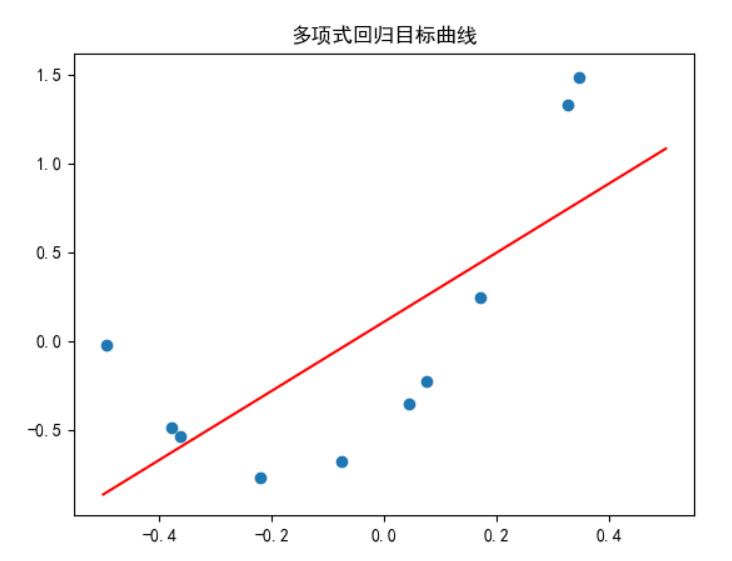
\includegraphics[height=6cm]{images/f000017}
\end{figure}
参数值为:
\begin{figure}[H]
	\caption{多项式回归最高次为1次学习的参数值}
	\label{f000018}
	\centering
	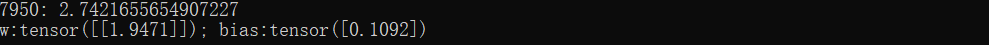
\includegraphics[width=15cm]{images/f000018}
\end{figure}
由上图可以看出,只用一条直线,不可能拟合出图中的数据点。这就是深度学习中的欠拟合(Under-Fitting)问题,当模型的表现能力低于数据集的实际分布函数时,就会出现这种情况。例如在本例中,拟合的函数为二次,我们硬要使用一次函数来拟合,结果就是不能很好的拟合。\newline
当最高次为2次时,运行结果如下所示:
\begin{figure}[H]
	\caption{多项式回归最高次为2次运行结果图}
	\label{f000019}
	\centering
	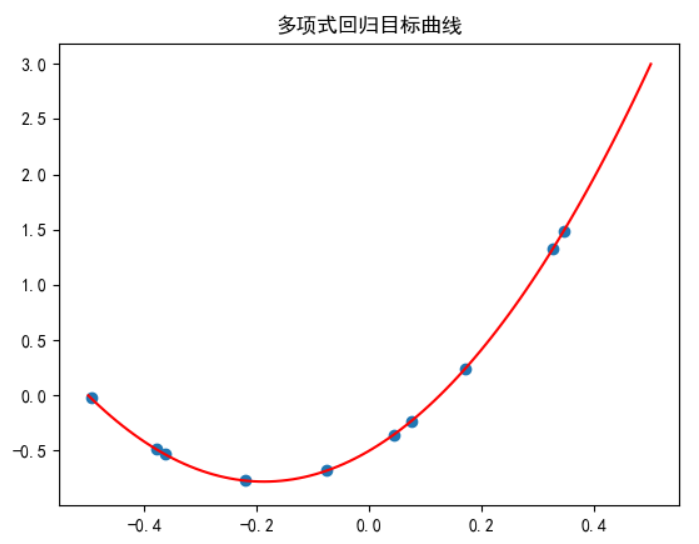
\includegraphics[height=6cm]{images/f000019}
\end{figure}
学习到的参数为:
\begin{figure}[H]
	\caption{多项式回归最高次为2次学习的参数值}
	\label{f000020}
	\centering
	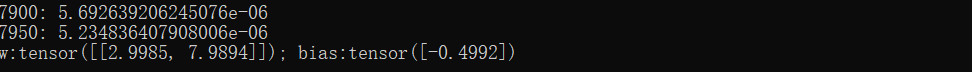
\includegraphics[width=15cm]{images/f000020}
\end{figure}
由上面可以看出,由于实际数据是二次函数,而我们的模型也是二次函数,所以无论从图形上看,还是从学习到的参数上看,都非常好的拟合了原曲线。
当最高次为9次时,运行结果如下所示:
\begin{figure}[H]
	\caption{多项式回归最高次为9次运行结果图}
	\label{f000021}
	\centering
	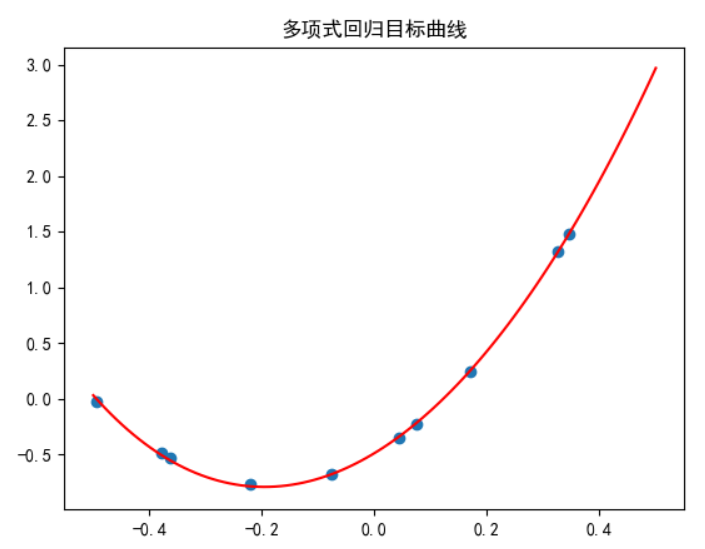
\includegraphics[height=6cm]{images/f000021}
\end{figure}
学习到的参数为:
\begin{figure}[H]
	\caption{多项式回归最高次为9次学习的参数值}
	\label{f000022}
	\centering
	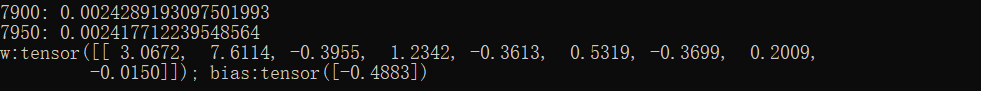
\includegraphics[width=15cm]{images/f000022}
\end{figure}
从上面的结果来看,我们9次多项式在图像上看,也可以较好的拟合数据点,但是所学到的参数,就和目标值比起来有些差距了,而且运算量也比二次时要大得多。并且我们为了演示效果,我们只选取的$[-0.5, 0.5]$这一个小的区域,如果将区域放大,那么拟合的效果就会更差。\newline
综上所述,我们选择与实际问题相匹配的模型复杂度,对于解决实际问题是非常重要的。
\subsection{总结}
在本章中,我们向大家详细介绍了线性回归的数学原理,同时还介绍了怎样用解析法求解线性回归问题。接着我们利用标准的PyTorch方式,求解了线性回归问题。我们同时讨论了所拟合的函数不是线性回归的情况,我们以二次函数为例,并分别用1次、2次、9次多项式来拟合,发现2次多项式的效果最好,因此得出需要找到与实际问题相匹配的模型,对于解决实际问题非常重要。






\newpage
\maketitle
\begin{center}
\Large \textbf{第4章 逻辑回归} \quad \textbf{}
\end{center}
\begin{abstract}
在本章中我们将讨论分类问题,介绍二分类和多分类问题,也就是逻辑回归和softmax回归。
\end{abstract}
\section{逻辑回归概述}
从本章开始,将正式进入深度学习领域。逻辑回归算法是最简单的一种模式识别算法,虽然其仅能解决线性可分的问题,但是由于其较简单,故当前还在大量使用。例如在医学诊断中,每个疾病都是由一系列症状和综合特征组成的,对于每一位患者,只要准确地收集其症状和综合特征,利用逻辑回归算法就能做出医学专家水准的诊断。由此可见,逻辑回归算法的威力还是相当强大的。
在本章中,将首先研究逻辑回归算法的数学基础,然后以MNIST手写数字识别为例,介绍这个数据的格式,以及怎样用逻辑回归算法进行MNIST手写数字识别,并且训练模型,使其达到1\%左右的误差率。
\subsection{数学基础}
\subsubsection{直观解释}
逻辑回归算法虽然是非常简单的机器学习算法,但是其数学基础还是比较复杂的。如果刚开始就陷入算法的数学细节中,则很难理解逻辑回归问题的本质,最后只是一堆数学公式,而不知道具体该怎么应用到实际问题中。这种现象是我们应该着力避免的。\newline
所以先不考虑数学理论,而是讲一下逻辑回归算法的物理意义,使读者对逻辑回归算法有一个直观的了解,为对后续数学理论的理解打下基础。\newline
下面通过一个简单的例子来说明什么是逻辑回归算法。假设在三维空间中有一组待分类的点,同时有一系列平面代表这些点应该属于的类别,我们将通过这些点到代表类别的平面的距离,来判断点属于的类别。也就是说,对于一个点来说,我们找到与其距离最近的平面,那么就说这个点属于这个类别。上面的讨论是在三维空间下进行的,如果推广到多维空间,那么这里的平面就变成了超平面,但是概念是类似的。\newline
将上述描述转换成数学语言:假设输入向量为$\boldsymbol{x}$,其维数为$D$,输出类别为$\boldsymbol{y}$,共有$N$个类别。对于上面的分类问题,如果把问题简化,就变为在二维平面上的点及一系列代表类别的线,求距离该点最近的直线的问题,而直线在二维情况下可以表示为$y=wx + b$,其中$w$为权重,$b$为偏移量。如果将上式推广到高维空间,则权值将变为一个矩阵,偏移量将变为一个向量,可以表示为$W\boldsymbol{x} + \boldsymbol{b}$,我们将权值矩阵和偏移量向量称为模型的参数集。
\subsubsection{数学推导}
有了对逻辑回归问题的直观理解之后,开始推导逻辑回归算法。首先讲解单类别逻辑回归问题,如判断患者是否患有某种疾病。然后讨论多类别逻辑回归问题,因为在MNIST手写数字识别的例子中,需要判断给定图片是0~9中的哪个数字,就是一个多类别模式识别问题。\newline
与线性回归算法类似,下面除了讲述普通迭代法求解,还会讲解利用牛顿法解决逻辑回归问题。通常牛顿法收敛速度更快。\newline
在本章理论部分的最后,会简单讨论一下通用学习模型,因为线性回归和逻辑回归算法都是这种通用学习模型的特例,而且利用通用学习模型,还可以推导出更多机器学习算法。\newline
对于模式分类(Classification)问题,训练样本中$y \in \{0,1\}$,假设就变为:
\begin{equation}
\hat{y} = h_{\boldsymbol{\theta}}(\boldsymbol{x}) \in \{0, 1\}
\label{lcrn-hx-def}
\end{equation}
其中$\boldsymbol{x} \in R^{n}$为特征向量。\newline
我们使用sigmoid函数来表示$\hat{y}=h_{\boldsymbol{\theta}}(\boldsymbol{x})$,选择Sigmoid函数并不是随意的,而是有理论基础的。在本节中,先假定是为了方便而选择Sigmoid函数。在后面通用机器学习部分,大家将看到这样做的原因。\newline
sigmoid函数定义为:
\begin{equation}
\sigma (z) = \frac{1}{1 + e^{-z}}, \quad z \in R
\label{lcrn-sigmoid-function-def}
\end{equation}
式中的$z$我们称之为线性输入和。Sigmoid函数曲线为:
\begin{figure}[H]
	\caption{sigmoid函数图像}
	\label{f000023}
	\centering
	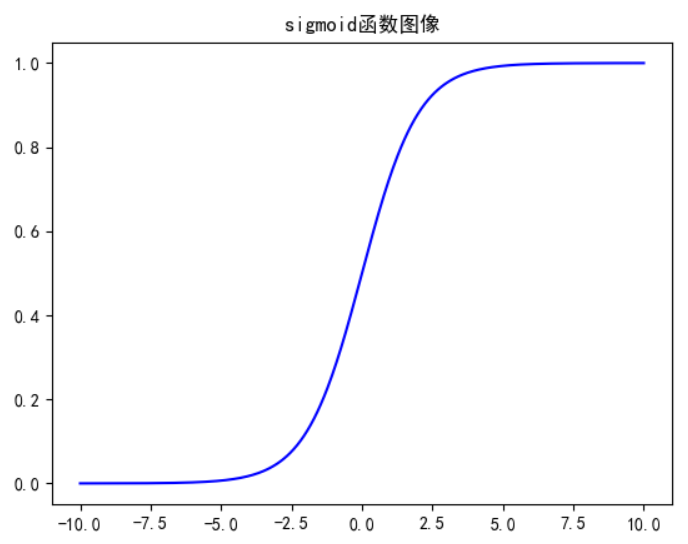
\includegraphics[height=6cm]{images/f000023}
\end{figure}
由于Sigmoid函数在深度学习中比较常用,并且经常用到其导数,下面我们来推导其导数形式:
\begin{equation}
\begin{aligned}
\sigma ' (z) = \frac{d(\frac{1}{1+e^{-z}})}{dz}= \frac{d(\frac{1}{1+e^{-z}})}{d(1+e^{-z})}\frac{d(1+e^{-z})}{dz} \\
= \Big( -\frac{1}{(1+e^{-z})^{2}} \Big)(-e^{-z})=\frac{e^{-z}}{(1+e^{-z})^{2}} \\
=\frac{1}{1+e^{-z}}\frac{e^{-z}}{1+e^{-z}}=\frac{1}{1+e^{-z}}\Big( 1 - \frac{1}{1+e^{-z}} \Big) \\
=\sigma(z)\Big( 1 - \sigma(z) \Big)
\end{aligned}
\label{lcrn-sigmoid-gradient-formula}
\end{equation}
在上式中,线性输入和定义为:
\begin{equation}
z = \boldsymbol{w}^{T} \cdot \boldsymbol{x} + b, \quad z \in R
\label{lcrn-z-def}
\end{equation}
其中权值参数$\boldsymbol{w} \in R^{n}$,输入信号$\boldsymbol{x} \in R^{n}$,$b \in R$为偏置值。与线性回归时的表示形式相同。\newline
我们可以将假设函数表示为:
\begin{equation}
\hat{y}=h_{\boldsymbol{\theta}} (\boldsymbol{x}) = \frac{1}{1 + e^{-\boldsymbol{w}^{T} \cdot \boldsymbol{x} - b}}
\label{lcrn-h-theta-def}
\end{equation}
由于我们研究的问题是一个二分类问题,目标值$y$只能取0或者1,下面我们来表示出$y=0$和$y=1$事件:
\begin{equation}
\begin{aligned}
P(y=1 \vert \boldsymbol{x}; \boldsymbol{\theta}) = \hat{y} \\
P(y=0 \vert \boldsymbol{x}; \boldsymbol{\theta}) = 1 - \hat{y}
\end{aligned}
\label{lcrn-y0-y1-def}
\end{equation}
在实际应用中,我们经常将上面的两个式子简化为一个式子:
\begin{equation}
P(y \vert \boldsymbol{x}; \boldsymbol{\theta}) =  \hat{y}^{y} ( 1 - \hat{y} )^{1-y}
\label{lcrn-y0-y1-merged}
\end{equation}
对上式可以这样理解,对于$y=1$,等式右边第二项的指数值为0,其值为1,所以就剩下第一项;而$y=0$时,等式右边第一项的指数值为0,其值为1,则只剩下第二项,所以与用两个等式表达的结果相同。\newline
假设我们连续进行$m$次实验,每次实验均可能取0或者1,我们称这些实验结果出现的概率为似然函数:
\begin{equation}
\mathcal{L}(\boldsymbol{\theta}) = \prod_{i=1}^{m} P( y^{(i)} \vert \boldsymbol{x}^{(i)}; \boldsymbol{\theta} )
\label{lcrn-likelyhood-function-def}
\end{equation}
这时我们的任务就是调整参数$\boldsymbol{\theta}$使得出现上面结果的概率最大,这就是最大似然算法。\newline
在上式中是连乘形式,在实际中很难处理,由于我们知道对一个正数取对数,其相对值的大小不变,所以我们可以对上式取对数,得到对数似然函数:
\begin{equation}
l(\boldsymbol{\theta}) = \log \mathcal{L}(\boldsymbol{\theta}) = \sum_{i=1}^{m} \log P( y^{(i)} \vert \boldsymbol{x}^{(i)}; \boldsymbol{\theta} )
\label{lcrn-log-likelyhood-function-def}
\end{equation}
将式\ref{lcrn-y0-y1-merged}代入式\ref{lcrn-log-likelyhood-function-def}可得:
\begin{equation}
\begin{aligned}
l(\boldsymbol{\theta}) = \sum_{i=1}^{m} \log P( y^{(i)} \vert \boldsymbol{x}^{(i)}; \boldsymbol{\theta} ) \\
= \sum_{i=1}^{m} \log \Big(  (\hat{y}^{(i)})^{y^{(i)}} ( 1 - \hat{y}^{(i)} )^{1-y^{(i)}} \Big) \\
= \sum_{i=1}^{m} \Big( y^{(i)} \log \hat{y}^{(i)} + (1-y^{(i)})\log(1 - \hat{y}^{(i)}) \Big)
\end{aligned}
\label{lcrn-log-likelyhood-function-simplified}
\end{equation}
在实际应用中,我们通常喜欢求最小值,所以我们常用负数似然函数:
\begin{equation}
l(\boldsymbol{\theta}) = \sum_{i=1}^{m} \Big( -y^{(i)} \log \hat{y^{(i)}} - (1-y^{(i)})\log(1 - \hat{y}^{(i)}) \Big)
\label{lcrn-negative-log-likelyhood-function-simplified}
\end{equation}
我们定义:
\begin{equation}
\nabla_{\boldsymbol{\theta}} l(\boldsymbol{\theta}) = \frac{\partial{l(\boldsymbol{\theta})}}{\partial{\boldsymbol{\theta}}}
\label{lcrn-nll-gradient-symbol}
\end{equation}
网络操作的更新公式为:
\begin{equation}
\boldsymbol{\theta} \leftarrow \boldsymbol{\theta} - \alpha \nabla_{\boldsymbol{\theta}} l(\boldsymbol{\theta})
\label{lcrn-parameter-update-formala}
\end{equation}
式中$0<\alpha<1$,是学习率。\newline
代价函数值$\nabla_{\boldsymbol{\theta}}l(\boldsymbol{\theta}) \in R$,网络参数为权值参数$\boldsymbol{w} \in R^{n}$和偏置值$b$。\newline
代价函数值对权值参数导数为:
\begin{equation}
\frac{ \partial{l(\boldsymbol{\theta})} }{ \boldsymbol{w} } = \begin{bmatrix}
\frac{ \partial{l(\boldsymbol{\theta})} } { w_{1} } && \frac{ \partial{l(\boldsymbol{\theta})} } { w_{2} } & ... & \frac{ \partial{l(\boldsymbol{\theta})} } { w_{n} }
\end{bmatrix}
\label{lcrn-nll-vs-w-gradient-vector}
\end{equation}
上式中第$j$项为:
\begin{equation}
\begin{aligned}
\frac{ \partial{l(\boldsymbol{\theta})} } { \partial{w_{j}} } = \frac{ \partial{ \sum_{i=1}^{m} \Big( -y^{(i)} \log \hat{y}^{(i)} - (1-y^{(i)})\log(1 - \hat{y}^{(i)}) \Big) } } { \partial{w_{j}} } \quad (1) \\
=\sum_{i=1}^{m} -\frac{\partial{y^{(i)} \log \hat{y}^{(i)}}}{ \partial{w_{j}}} - \frac{\partial{ (1-y^{(i)})\log(1 - \hat{y}^{(i)}) }}{ \partial{w_{j}}} \quad (2) \\
= \sum_{i=1}^{m} \bigg(-\frac{\partial{y^{(i)} \log \sigma(\boldsymbol{w}^{T} \cdot \boldsymbol{x}^{(i)} + b) }}{ \partial{w_{j}}}- \frac{\partial{ (1- \sigma(\boldsymbol{w}^{T} \cdot \boldsymbol{x}^{(i)} + b))\log(1 - \hat{y}^{(i)}) }}{ \partial{w_{j}}} \bigg) \quad (3) \\
= \sum_{i=1}^{m} \bigg(-\frac{\partial{y^{(i)} \log \sigma(\boldsymbol{w}^{T} \cdot \boldsymbol{x}^{(i)} + b) }}{\partial{\sigma(\boldsymbol{w}^{T} \cdot \boldsymbol{x}^{(i)} + b)}} \frac{\partial{\sigma(\boldsymbol{w}^{T} \cdot \boldsymbol{x}^{(i)} + b)}}{\partial{(\boldsymbol{w}^{T} \cdot \boldsymbol{x}^{(i)} + b)}}  \frac{\partial{(\boldsymbol{w}^{T} \cdot \boldsymbol{x}^{(i)} + b)}}{ \partial{w_{j}}} \\
- \frac{\partial{ (1- y)\log(1 - \sigma(\boldsymbol{w}^{T} \cdot \boldsymbol{x}^{(i)} + b)) }}{\partial{\sigma(\boldsymbol{w}^{T} \cdot \boldsymbol{x}^{(i)} + b)}} \frac{\partial{\sigma(\boldsymbol{w}^{T} \cdot \boldsymbol{x}^{(i)} + b)}}{\partial{(\boldsymbol{w}^{T} \cdot \boldsymbol{x}^{(i)} + b)}}  \frac{\partial{(\boldsymbol{w}^{T} \cdot \boldsymbol{x}^{(i)} + b)}}{ \partial{w_{j}}} \bigg) \quad (4) \\
= \sum_{i=1}^{m} \Big( -y^{(i)}\frac{1}{\sigma(\boldsymbol{w}^{T} \cdot \boldsymbol{x}^{(i)} + b)}\sigma(\boldsymbol{w}^{T} \cdot \boldsymbol{x}^{(i)} + b)(1-\sigma(\boldsymbol{w}^{T} \cdot \boldsymbol{x}^{(i)} + b))x_{j}^{(i)} \\
- (1-y^{(i)})\frac{-1}{1 - \sigma(\boldsymbol{w}^{T} \cdot \boldsymbol{x}^{(i)} + b)}\sigma(\boldsymbol{w}^{T} \cdot \boldsymbol{x}^{(i)} + b)(1-\sigma(\boldsymbol{w}^{T} \cdot \boldsymbol{x}^{(i)} + b))x_{j}^{(i)} \Big) \quad (5)\\
= \sum_{i=1}^{m} \Big( -y^{(i)}(1-\sigma(\boldsymbol{w}^{T} \cdot \boldsymbol{x}^{(i)} + b))x_{j}^{(i)} \\
+(1-y^{(i)})\sigma(\boldsymbol{w}^{T} \cdot \boldsymbol{x}^{(i)} + b)x_{j}^{(i)}  \Big) \quad (6) \\
= \sum_{i=1}^{m} \Big( \sigma(\boldsymbol{w}^{T} \cdot \boldsymbol{x}^{(i)} + b) - y^{(i)} \Big)x_{j}^{(i)}
\end{aligned}
\label{lcrn-nll-vs-wj-gradient}
\end{equation}
接下来我们来求代价函数对偏置值的微分:
\begin{equation}
\begin{aligned}
\frac{ \partial{l(\boldsymbol{\theta})} } { \partial{b} } = \frac{ \partial{ \sum_{i=1}^{m} \Big( -y^{(i)} \log \hat{y}^{(i)} - (1-y^{(i)})\log(1 - \hat{y}^{(i)}) \Big) } } { \partial{b} } \quad (1) \\
=\sum_{i=1}^{m} -\frac{\partial{y^{(i)} \log \hat{y}^{(i)}}}{ \partial{b}} - \frac{\partial{ (1-y^{(i)})\log(1 - \hat{y}^{(i)}) }}{ \partial{b}} \quad (2) \\
= \sum_{i=1}^{m} \bigg(-\frac{\partial{y^{(i)} \log \sigma(\boldsymbol{w}^{T} \cdot \boldsymbol{x}^{(i)} + b) }}{ \partial{b}}- \frac{\partial{ (1- \sigma(\boldsymbol{w}^{T} \cdot \boldsymbol{x}^{(i)} + b))\log(1 - \hat{y}^{(i)}) }}{ \partial{b}} \bigg) \quad (3) \\
= \sum_{i=1}^{m} \bigg(-\frac{\partial{y^{(i)} \log \sigma(\boldsymbol{w}^{T} \cdot \boldsymbol{x}^{(i)} + b) }}{\partial{\sigma(\boldsymbol{w}^{T} \cdot \boldsymbol{x}^{(i)} + b)}} \frac{\partial{\sigma(\boldsymbol{w}^{T} \cdot \boldsymbol{x}^{(i)} + b)}}{\partial{(\boldsymbol{w}^{T} \cdot \boldsymbol{x}^{(i)} + b)}}  \frac{\partial{(\boldsymbol{w}^{T} \cdot \boldsymbol{x}^{(i)} + b)}}{ \partial{b}} \\
- \frac{\partial{ (1- y)\log(1 - \sigma(\boldsymbol{w}^{T} \cdot \boldsymbol{x}^{(i)} + b)) }}{\partial{\sigma(\boldsymbol{w}^{T} \cdot \boldsymbol{x}^{(i)} + b)}} \frac{\partial{\sigma(\boldsymbol{w}^{T} \cdot \boldsymbol{x}^{(i)} + b)}}{\partial{(\boldsymbol{w}^{T} \cdot \boldsymbol{x}^{(i)} + b)}}  \frac{\partial{(\boldsymbol{w}^{T} \cdot \boldsymbol{x}^{(i)} + b)}}{ \partial{b}} \bigg) \quad (4) \\
= \sum_{i=1}^{m} \Big( -y^{(i)}\frac{1}{\sigma(\boldsymbol{w}^{T} \cdot \boldsymbol{x}^{(i)} + b)}\sigma(\boldsymbol{w}^{T} \cdot \boldsymbol{x}^{(i)} + b)(1-\sigma(\boldsymbol{w}^{T} \cdot \boldsymbol{x}^{(i)} + b)) \\
- (1-y^{(i)})\frac{-1}{1 - \sigma(\boldsymbol{w}^{T} \cdot \boldsymbol{x}^{(i)} + b)}\sigma(\boldsymbol{w}^{T} \cdot \boldsymbol{x}^{(i)} + b)(1-\sigma(\boldsymbol{w}^{T} \cdot \boldsymbol{x}^{(i)} + b)) \Big) \quad (5)\\
= \sum_{i=1}^{m} \Big( -y^{(i)}(1-\sigma(\boldsymbol{w}^{T} \cdot \boldsymbol{x}^{(i)} + b)) \\
+(1-y^{(i)})\sigma(\boldsymbol{w}^{T} \cdot \boldsymbol{x}^{(i)} + b)  \Big) \quad (6) \\
= \sum_{i=1}^{m} \Big( \sigma(\boldsymbol{w}^{T} \cdot \boldsymbol{x}^{(i)} + b) - y^{(i)} \Big)
\end{aligned}
\label{lcrn-nll-vs-b-gradient}
\end{equation}
对权值参数的更新公式为:
\begin{equation}
w_{j} \leftarrow w_{j} - \alpha \frac{\partial{l(\boldsymbol{\theta})}}{\partial{w_{j}}}, \quad j \in \{1, 2, ..., n\}
\label{lcrn-wj-update}
\end{equation}
对偏置值的更新公司为:
\begin{equation}
b \leftarrow b - \alpha \frac{\partial{l(\boldsymbol{\theta})}}{\partial{b}}
\label{lcrn-b-update}
\end{equation}
如果我们用$\boldsymbol{\theta}$来表示网络参数,则可以有如下参数更新公式:
\begin{equation}
\theta_{j} \leftarrow \theta_{j} - \alpha \frac{\partial{l(\boldsymbol{\theta})}}{\partial{\theta_{j}}}=\theta_{j} - \alpha (\hat{y}^{(i)} - y^{(i)})x_{j}, \quad j \in \{1, 2, ..., n\}
\label{lcrn-thetaj-update}
\end{equation}
上式与线性回归算法中的随机梯度下降算法的学习公式非常相似,那么它们是一类函数吗?答案是否定的。因为在上式中,$\hat{y}^{(i)}$是非线性的Sigmoid函数,所以两个公式虽然外形上有点儿相似,但却是两种不同的算法。
\subsubsection{牛顿法}
在线性回归算法中,除了使用迭代算法,还可以使用解析法,即最小二乘法求出参数解。但是在逻辑回归中,假设函数使用的是指数函数,所以很难用解析法求出解。但是还有更好的算法,使收敛速度更快,这就是下面要介绍的牛顿法。\newline
先来介绍一下标准的牛顿法,然后再介绍牛顿法在逻辑回归算法中的应用。假设给定一个函数映射$f:R \to R$,我们的任务是发现一点$x$使$f(x)=0$,用牛顿法求解这个问题的公式:
\begin{equation}
x \leftarrow x - \frac{f(x)}{f'(x)}
\label{lcrn-newton-method}
\end{equation}
只介绍定义会令人感觉很抽象。下面用一个具体的例子来讲解牛顿法的具体算法,使读者对牛顿法有一个直观的认识。\newline
我们假设有一个函数:
\begin{equation}
f(x)=x^{2} - 2.25
\label{lcrn-newton-method-demo-function}
\end{equation}
我们知道,其与$x$轴交点为$x=1.5$,假设现在的任务就是给定$f(x)$,以及任意初始值点$x_{0}=4.5$,求出$f(x)=0$点的坐标,这就是牛顿法要解决的问题。\newline
根据牛顿法,从$x_{0}=4.5$处做切线,如下图所示:
\begin{figure}[H]
	\caption{过$x_{0}$点切线示意图}
	\label{f000024}
	\centering
	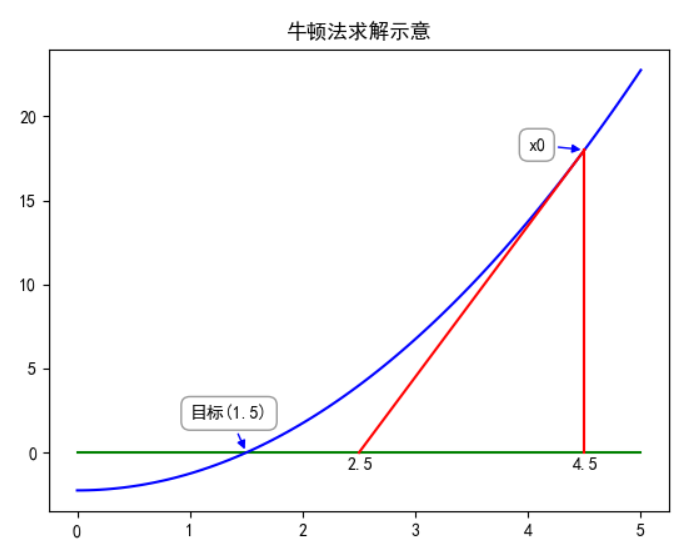
\includegraphics[height=10cm]{images/f000024}
\end{figure}
我们在$x_{0}$点处作曲线的切线,与$x$轴相交于$x_{1}$点,做曲线过$x_{1}$点切线,与$x$轴相交于$x_{2}$,如下图所示:
\begin{figure}[H]
	\caption{过$x_{1}$点切线示意图}
	\label{f000025}
	\centering
	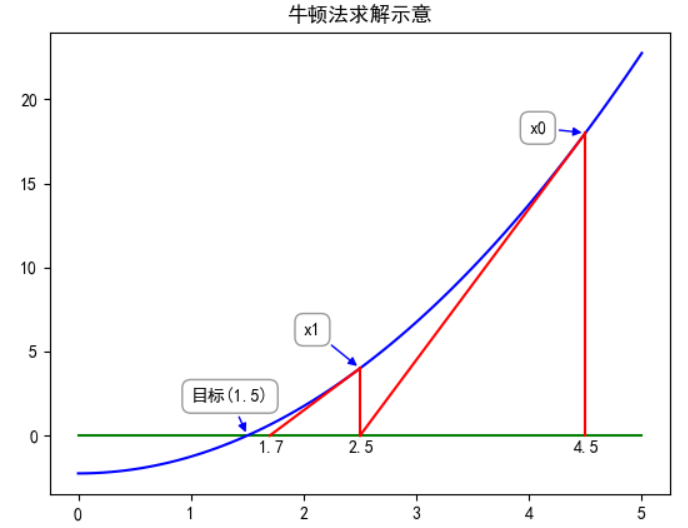
\includegraphics[height=10cm]{images/f000025}
\end{figure}
此时得到的值$x_{2}$即为1.7,而这个函数与X轴交点的真实坐标为1.5,我们仅通过两次迭代,就已经非常接近真实值了。我们相信,如果再连续应用一两次牛顿法,就可以得到1.5这个正确值。\newline
从上面的例子可以看出,用牛顿法迭代求值时,可以证明其是以平方的速度向真值点逼近的,如果在离真值点很近的地方,如本次迭代点离真值点的距离为0.1,那么经过一次迭代之后,其距离将变为0.01,再经过一次迭代,其距离将进一步缩小为0.0001。由此可见,其收敛速度是相当快的。\newline
上述图形的生成代码:
\lstset{language=PYTHON, caption={牛顿法求解示意图(app/pytorch/book/chp003/chp003\_c002.py)}, label={lcrn-newton-method-graph-draw}}
\begin{lstlisting}
class Chp003C002(object):
    def __init__(self):
        self.name = ''

    def run(self):
        plt.rcParams['font.sans-serif'] = ['SimHei']
        plt.rcParams['axes.unicode_minus'] = False
        plt.title('牛顿法求解示意')
        self.draw_curve()
        self.draw_x0()
        self.draw_x1()
        plt.show()
    
    def draw_curve(self):
        # 绘制x轴
        xx = np.array([0.0, 5.0])
        xy = np.array([0.0, 0.0])
        plt.plot(xx, xy, '-g')
        # 绘制曲线
        x = np.linspace(0, 5, 100)
        y = x*x - 2.25
        plt.plot(x, y, '-b')
        plt.annotate(s=r'目标(1.5)',xy=(1.5, 0.0),\
            xytext=(1.0,2.0),weight='bold',color='black',\
            arrowprops=dict(arrowstyle='-|>',\
            connectionstyle='arc3',color='blue'),\
            bbox=dict(boxstyle='round,pad=0.5', fc='white', \
            ec='k',lw=1 ,alpha=0.4))

    def draw_x0(self):
        # x0点垂线
        x00x = np.array([4.5, 4.5])
        x00y = np.array([0.0, 4.5*4.5-2.25])
        plt.plot(x00x, x00y, '-r')
        plt.annotate(s=r'x0',xy=(4.5, 4.5*4.5-2.25),
            xytext=(4.0,18.0),weight='bold',color='black',\
            arrowprops=dict(arrowstyle='-|>',\
            connectionstyle='arc3',color='blue'),\
            bbox=dict(boxstyle='round,pad=0.5', fc='white', \
            ec='k',lw=1 ,alpha=0.4))
        plt.text(4.4, -1.0, '4.5')
        # x0点处切线并与x轴相交
        x01x = np.array([4.5, 2.5])
        x01y = np.array([4.5*4.5-2.25, 0])
        plt.plot(x01x, x01y, '-r')
        plt.text(2.4, -1.0, '2.5')

    def draw_x1(self):
        # x1点垂线
        x10x = np.array([2.5, 2.5])
        x10y = np.array([0.0, 2.5*2.5-2.25])
        plt.plot(x10x, x10y, '-r')
        plt.annotate(s=r'x1',xy=(2.5, 2.5*2.5-2.25),\
            xytext=(2.0,6.0),weight='bold',color='black',\
            arrowprops=dict(arrowstyle='-|>',\
            connectionstyle='arc3',color='blue'),\
            bbox=dict(boxstyle='round,pad=0.5', fc='white', \
            ec='k',lw=1 ,alpha=0.4))
        # x1点切线
        x11x = np.array([2.5, 1.7])
        x11y = np.array([2.5*2.5-2.25, 0])
        plt.plot(x11x, x11y, '-r')
        plt.text(1.6, -1.0, '1.7')
\end{lstlisting}
在上述代码中,我们略去了切线方程的求解,以及求出切线方程与x轴的交点,这些部分的计算大家可以自己完成并验证,由于这部分代码与深度学习无关,这里就不进行过多解释了。\newline
下面来讨论,怎样将牛顿法应用于逻辑回归问题的求解过程。\newline
在逻辑回归算法中,需要求出负对数似然函数$l(\boldsymbol{\theta})$的最大值,根据高等数学知识可以知道,求极值点就等于求对数似然函数导数为0的点,如果把$l'(\boldsymbol{\theta})$视为上面讨论中的$f(x)$,则就可以针对$l'(\boldsymbol{\theta})$应用牛顿法,公式为:
\begin{equation}
\theta \leftarrow \theta - \frac{l'(\boldsymbol{\theta})}{l''(\boldsymbol{\theta})}
\label{lcrn-nll-newton-method}
\end{equation}
应用牛顿法可以更快地求出$l$的极值。\newline
在前述公式推导中,并没有强调实际上我们的特征值是$n$维的,所以输入信号为$n$维的,所以输入信号为n维向量$\boldsymbol{x} \in R^{n}$,参数同样是$n$维向量$\boldsymbol{\theta} \in R^{n}$,因此我们需要牛顿法的向量形式。\newline
我们首先将偏置$b$作为$\theta _{0}$,如下所示:
\begin{equation}
\boldsymbol{\theta} = \begin{bmatrix}
\theta _{0} \\
\theta _{1} \\
\theta _{2} \\
...\\
\theta _{n}
\end{bmatrix} = \begin{bmatrix}
b \\
\theta _{1} \\
\theta _{2} \\
... \\
\theta _{n} \\
\end{bmatrix} \in R^{n+1}
\label{lcrn-theta-modified-for-newton-vector-method}
\end{equation}
同理我们在特征向量加入$x_{0}=1$项,如下所示:
\begin{equation}
\boldsymbol{x} = \begin{bmatrix}
x _{0} \\
x _{1} \\
x _{2} \\
...\\
x _{n}
\end{bmatrix} = \begin{bmatrix}
1 \\
x _{1} \\
x _{2} \\
... \\
x _{n} \\
\end{bmatrix} \in R^{n+1}
\label{lcrn-x-modified-for-newton-vector-method}
\end{equation}
则牛顿法的向量形式可以表示为:
\begin{equation}
\theta ^{T} \leftarrow \theta - H^{-1} \Big(\nabla _{\boldsymbol{\theta}} l(\boldsymbol{\theta}) \Big)^{T}
\label{lcrn-newton-vector-method}
\end{equation}
其中代价函数对参数的微分定义为:
\begin{equation}
\nabla _{\boldsymbol{\theta}} l(\boldsymbol{\theta}) = \begin{bmatrix}
\frac{\partial{l(\boldsymbol{\theta})}}{\partial{\theta _{0}}} & \frac{\partial{l(\boldsymbol{\theta})}}{\partial{\theta _{1}}} & \frac{\partial{l(\boldsymbol{\theta})}}{\partial{\theta _{2}}} & ... & \frac{\partial{l(\boldsymbol{\theta})}}{\partial{\theta _{n}}}
\end{bmatrix} \in R^{1 \times (n+1)}
\label{lcrn-loss-theta-gradient}
\end{equation}
式中$H^{-1}$为海森矩阵求逆,海森矩阵定义如下所示:
\begin{equation}
H = \begin{bmatrix}
\frac{\partial{l^{2}(\boldsymbol{\theta})}}{\partial{\theta _{0}\theta _{0}}} & \frac{\partial{l^{2}(\boldsymbol{\theta})}}{\partial{\theta _{0}\theta _{1}}} & \frac{\partial{l^{2}(\boldsymbol{\theta})}}{\partial{\theta _{0}\theta _{2}}} & ... & \frac{\partial{l^{2}(\boldsymbol{\theta})}}{\partial{\theta _{0}\theta _{n}}} \\
\frac{\partial{l^{2}(\boldsymbol{\theta})}}{\partial{\theta _{1}\theta _{0}}} & \frac{\partial{l^{2}(\boldsymbol{\theta})}}{\partial{\theta _{1}\theta _{1}}} & \frac{\partial{l^{2}(\boldsymbol{\theta})}}{\partial{\theta _{1}\theta _{2}}} & ... & \frac{\partial{l^{2}(\boldsymbol{\theta})}}{\partial{\theta _{1}\theta _{n}}} \\
\frac{\partial{l^{2}(\boldsymbol{\theta})}}{\partial{\theta _{2}\theta _{0}}} & \frac{\partial{l^{2}(\boldsymbol{\theta})}}{\partial{\theta _{2}\theta _{1}}} & \frac{\partial{l^{2}(\boldsymbol{\theta})}}{\partial{\theta _{2}\theta _{2}}} & ... & \frac{\partial{l^{2}(\boldsymbol{\theta})}}{\partial{\theta _{2}\theta _{n}}} \\
... \\
\frac{\partial{l^{2}(\boldsymbol{\theta})}}{\partial{\theta _{n}\theta _{0}}} & \frac{\partial{l^{2}(\boldsymbol{\theta})}}{\partial{\theta _{n}\theta _{1}}} & \frac{\partial{l^{2}(\boldsymbol{\theta})}}{\partial{\theta _{n}\theta _{2}}} & ... & \frac{\partial{l^{2}(\boldsymbol{\theta})}}{\partial{\theta _{n}\theta _{n}}} \\
\end{bmatrix} \in R^{(n+1) \times (n+1)}
\label{lcrn-hessian-matrix-def}
\end{equation}
通常,即在逻辑回归算法中,在特征向量的维数不太高的情况下,例如在几百个特征之内,利用牛顿法求解的速度还是相当快的。但是如果特征数量太多,有成千上万维,因为算法需要对海森矩阵求逆,所以运算量会比较大,使用牛顿法也就不太适合了,迭代算法可能具有更好的性能。
\subsubsection{通用学习模型}
到目前为止,我们学习了两种学习算法,分别是线性回归算法和逻辑回归算法,其中线性回归算法用于解决数值预测问题,而逻辑回归算法用于模式分类问题。其实这两种算法都是由所谓的通用线性模型(GLM)派生出来的,而且通用线性模型不仅可以派生出线性回归算法和逻辑回归算法,还可以派生出很多其他的主流算法。\newline
对于线性回归问题,可以将其表示为:
\begin{equation}
P(y \vert \boldsymbol{x}; \boldsymbol{\theta}), \quad y \in R, \quad (y \vert \boldsymbol{x}; \boldsymbol{\theta}) \sim \mathcal{N}(\boldsymbol{\mu}, \Sigma)
\label{lcrn-linear-regression-def}
\end{equation}
上式第一部分表示给定样本$\boldsymbol{x}$并以$\boldsymbol{\theta}$为参数情况下某个$y$值出现的概率,我们可以认为,由于研究的问题具有随机性,即使相同的$\boldsymbol{x}$也会出现不同的$y$值,而不同$y$值出现的概率不同。第二部分表示以$\boldsymbol{\theta}$为参数,$y$的分布符合均值为$\boldsymbol{\mu}$方差为$\Sigma$的高斯分布。\newline
由概率论的知识可以知道,一元高斯分布(Gaussian)的概率密度函数为:
\begin{equation}
f(x)=\frac{1}{\sqrt{2\pi}\sigma}e^{ -\frac{(x-\mu)^{2}}{2\sigma ^{2}} }
\label{lcrn-gaussian-uni-def}
\end{equation}
其图像如下所示:
\begin{figure}[H]
	\caption{一元高斯分布函数图像}
	\label{f000026}
	\centering
	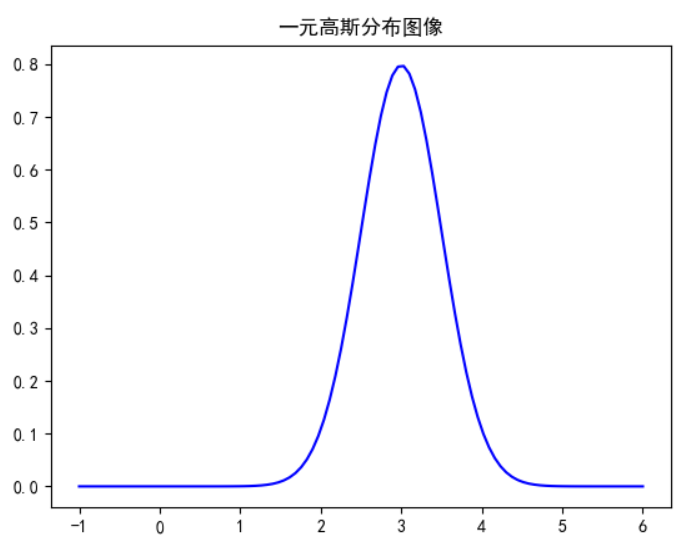
\includegraphics[height=6cm]{images/f000026}
\end{figure}
?????????????????? 加入二元高斯分布图像 ?????????????????
根据以上假设,可以得到线性回归算法,同时可以推导出最小二乘法,这在线性回归算法部分已经详细推导过,这里就不再赘述了。\newline
对于逻辑回归问题,我们定义:
\begin{equation}
P(y \vert \boldsymbol{x}; \boldsymbol{\theta}) = \phi
\label{lcrn-lcrn-prob}
\end{equation}
表示给定样本$\boldsymbol{x}$并以$\theta$为参数情况下,$y \in \{0, 1\}$出现的概率。其中$y$符合伯努利分布$y \sim Bernulli(\phi)$。在这里我们也认为所研究的问题具有随机性,对于相同的输入样本$\boldsymbol{x}$,$y$可以取0或者1,但是符合伯努利分布。\newline
下面我们来证明,这两种情况实际可以统一于通用机器学习(GML)模型。\newline
下面引入通用线性模型,可以推导出上述两个函数均是这个函数的特殊情况,并且以这个模型为基础,还可以推导出其他有用的模型。\newline
首先定义一个指数族函数:
\begin{equation}
P(y;\boldsymbol{\eta}) = b(y)exp(\boldsymbol{\eta}^{T}T(y)-\alpha(\boldsymbol{\eta}))
\label{lcrn-exp-function-group}
\end{equation}
在上式中:
\begin{itemize}
\item $\boldsymbol{\eta}$:自然参数;
\item T(y):充分统计量,在通常情况下$T(y)=y$;
\end{itemize}
通过指定不同的$\alpha$、$b$和$T$,我们可以得到一族函数,这些函数以$\boldsymbol{\eta}$为参数,为指数族函数。
\paragraph{逻辑回归推导}
下面我们来推导逻辑回归过程。对于伯努利分布:
\begin{equation}
P(y \vert \boldsymbol{x}; \boldsymbol{\theta}), \quad y \sim Bernulli(\phi)
\label{lcrn-gml-bernulli}
\end{equation}
$y$的概率质量函数可以表示为:
\begin{equation}
\begin{aligned}
P(y \vert \boldsymbol{x}; \boldsymbol{\theta}) = \phi ^{y} (1-\phi)^{1-y} = \exp \Big( \log \phi ^{y} (1-\phi)^{1-y}  \Big) \\
=\exp \Big( y\log \phi + (1-y)\log (1-\phi) \Big) \\
= \exp \Big( y(\log \phi - \log (1-\phi)) + \log(1-\phi)\Big) \\
= \exp \Big( \log \frac{\phi}{1-\phi} y + \log (1-\phi) \Big)
\end{aligned}
\label{lcrn-gml-bernulli-pp}
\end{equation}
我们设定:
\begin{itemize}
\item $b(y)=1$;
\item $\eta = \log \frac{\phi}{1-\phi}$,此时$\eta$为标量;
\item $T(y)=y$;
\item $\alpha(\eta)=-\log(1-\phi)$
\end{itemize}
将上述假设条件代入式\ref{lcrn-gml-bernulli-pp},我们就可以看到其将变为通用机器学习模型的公式。\newline
我们来研究一下自然参数$\eta$,在伯努利分布下其值定义为:
\begin{equation}
\eta = \log \frac{\phi}{1-\phi}
\label{lcrn-gml-eta-def}
\end{equation}
我们可以解出伯努利分布的参数$\phi$的值:
\begin{equation}
\phi = \frac{1}{1+e^{-\eta}}
\label{lcrn-gml-eta-to-phi}
\end{equation}
如果我们定义$\eta=\boldsymbol{w}^{T}\boldsymbol{x} + b$,上式就变为我们讲逻辑回归时模型的公式。由此可见,逻辑回归是通用机器学习算法的一个特例。
\paragraph{线性回归}
在线性回归问题中,我们认为$y \sim \mathcal{N}(\mu, \sigma)$符合高斯分布,我们设$\mu=\boldsymbol{w}^{T}\boldsymbol{x} + b$作为其均值,其概率密度函数如下所示:
\begin{equation}
\begin{aligned}
P(y \vert \boldsymbol{x}; \boldsymbol{\theta}) = \frac{1}{\sqrt{2\pi}\sigma}e^{-\frac{(y-\mu)^{2}}{2\sigma ^{2}}} \\
= \frac{1}{\sqrt{2\pi}\sigma}e^{-\frac{y^{2}-2y\mu + \mu ^{2}}{2\sigma ^{2}}} \\
= \frac{1}{\sqrt{2\pi}\sigma}e^{-\frac{y^{2}}{2\sigma ^{2}}}e^{\frac{2y\mu - \mu ^{2}}{2\sigma ^{2}}} \\
= \frac{1}{\sqrt{2\pi}\sigma}e^{-\frac{y^{2}}{2\sigma ^{2}}}e^{(\frac{2y\mu}{2\sigma ^{2}} - \frac{\mu ^{2}}{2\sigma ^{2}})} \\
= \frac{1}{\sqrt{2\pi}\sigma}\exp(-\frac{y^{2}}{2\sigma ^{2}})\exp(\frac{2y\mu}{2\sigma ^{2}} - \frac{\mu ^{2}}{2\sigma ^{2}})
\end{aligned}
\label{lcrn-gml-linear-regression-derive}
\end{equation}
我们设定:
\begin{itemize}
\item $\eta = \mu$;
\item $T(y)=y$;
\item $a(\eta)=\frac{\mu ^{2}}{2\sigma ^{2}}==\frac{\eta ^{2}}{2\sigma ^{2}}$;
\item $b(y)=\frac{1}{\sqrt{2\pi}\sigma}exp(-\frac{y^{2}}{2\sigma ^{2}})$;
\end{itemize}
通过指定$\eta$、$T$、$\alpha$和$b$之后,式\ref{lcrn-gml-linear-regression-derive}就变为了通用机器学习模型(GML)的形式了,由此可见,线性回归也是通用机器学习模型的一个特例。
通过这种指数族分布,实际上可以得到很多分布。\newline
\begin{itemize}
\item 多项式(Multinomial)分布:例如在手写数字识别中,分为0~9共10种类别,其中只有一个类别为1,其余类别均为0;
\item 泊松分布(Poisson):通常用来估算数量,如估算网站访问量和点击率等,也属于指数族分布;
\item 伽码分布(Gamma):通常用于对时间间隔的建模,也是指数族分布的一种;
\end{itemize}
在讲述了通用线性模型之后,我们自然要问,怎样使用它呢?假设我们有一个微信公众号,想估算文章主题、更新频率、大V数量等参数对粉丝数增长的影响。对于粉丝数增长的问题,可以选用泊松分布(Poisson),因此下面的任务就是设计一种泊松回归算法,来解粉丝数增长估算问题。如果以通用线性模型为指导,通过选择恰当的参数,就可以很方便地得出相应的回归算法。
因为在本章的例子中,在使用MNIST手写数字识别的实例中,需要用到多项式分布情况,即输出类别为0~9共10个类别,采用softmax函数形式,所以下面就来推导一下多项式分布下的softmax函数。
\paragraph{通用机器学习模型总结}
在根据通用线性模型做具体的算法设计前,需要有以下3个前提条件:
\begin{enumerate}
\item $(y \vert \boldsymbol{x}; \boldsymbol{\theta})\sim \exp ^{*}(\boldsymbol{\eta})$:对于变量$y$在给定输入样本$\boldsymbol{x}$和模型参数$\boldsymbol{\theta}$情况下符合参数为$\boldsymbol{\eta}$的指数族分布;
\item 我们的目标是在给定输入信号$\boldsymbol{x}$的情况下,求出$T(y)$的希望值作为模型函数,即:
\begin{equation}
\hat{y}=E\Big[T(y) \vert \boldsymbol{x} \Big]=E\Big[y \vert \boldsymbol{x} \Big]
\label{lcrn-gml-yhat}
\end{equation}
因为在通常情况下我们都取$T(y)=y$;
\item 当输出值$y$为标量时,$\eta = \boldsymbol{\theta} \boldsymbol{x}$;如果输出值$\boldsymbol{y} \in R^{m}$时,$\boldsymbol{\eta}$为向量形式,此时参数$\Theta \in R^{m \times n}$为一个矩阵,如下所示:
\begin{equation}
\boldsymbol{\eta} = \Theta \boldsymbol{x} = \begin{bmatrix}
\boldsymbol{\Theta}_{1,}\boldsymbol{x} \\
\boldsymbol{\Theta}_{2,}\boldsymbol{x} \\
... \\
\boldsymbol{\Theta}_{m,}\boldsymbol{x}
\end{bmatrix}, \Theta_{i,} \in R^{1 \times n}
\label{lcrn-gml-eta-vector-formula}
\end{equation}
\end{enumerate}
\subparagraph{线性回归}
对于线性回归问题,我们假设$(y \vert \boldsymbol{x}; \boldsymbol{\theta}) \sim \mathcal{N}(\boldsymbol{\mu}, \Sigma)$的高斯分布(Gaussian),根据前面的推导,如果把高斯分布问题视为通用线性模型的指数族函数,则其参数如下:
\begin{equation}
\begin{aligned}
P(y \vert \boldsymbol{x}; \boldsymbol{\theta}) = b(y)\exp \Big( \eta ^{T}T(y) - \alpha(\eta) \Big)  \quad (1)\\
\eta = \mu  \quad (2) \\
T(y) = y \quad (3) \\
\alpha(\boldsymbol{\eta}) = \frac{\mu ^{2}}{2\sigma ^{2}} = \frac{\eta ^{2}}{2\sigma ^{2}} \quad (4) \\
b(y) = \frac{1}{\sqrt{2\pi}\sigma}\exp(-\frac{y^{2}}{2\sigma ^{2}}) \quad (5)
\end{aligned}
\label{lcrn-gml-linear-regression-summary}
\end{equation}
由上式中的第(2)行可以得到:
\begin{equation}
\hat{y} = E[\mu \vert \boldsymbol{x}; \boldsymbol{\theta}] = \eta = \boldsymbol{\theta} ^{T} \boldsymbol{x}
\label{lcrn-gml-linear-regression-summary-yhat}
\end{equation}
在上式中,我们将偏置值定义为$\theta _{0}=b$,有:
由上式中的第(2)行可以得到:
\begin{equation}
\boldsymbol{\theta} = \begin{bmatrix}
\theta _{0} \\
\theta _{1} \\
\theta _{2} \\
... \\
\theta _{n} 
\end{bmatrix} = \begin{bmatrix}
b \\
\theta _{1} \\
\theta _{2} \\
... \\
\theta _{n} 
\end{bmatrix} \in R^{n+1}
\label{lcrn-gml-linear-regression-summary-theta-b}
\end{equation}
将$x_{0} = 1$,有:
\begin{equation}
\boldsymbol{x} = \begin{bmatrix}
x_{0} \\
x_{1} \\
x_{2} \\
... \\
x _{n} 
\end{bmatrix} = \begin{bmatrix}
1 \\
x_{1} \\
x_{2} \\
... \\
x _{n} 
\end{bmatrix} \in R^{n+1}
\label{lcrn-gml-linear-regression-summary-x0}
\end{equation}
\subparagraph{逻辑回归}
逻辑回归是一个二分类问题,其中$y \in \{0, 1\}$只能取0或1两个值,其服从的是伯努利分布:
\begin{equation}
\begin{aligned}
P(y \vert \boldsymbol{x}; \boldsymbol{\theta}) = b(y)\exp \Big( \eta ^{T}T(y) - \alpha(\eta) \Big)  \quad (1)\\
P(y \vert \boldsymbol{x}; \boldsymbol{\theta}) = \phi ^{y} (1-\phi)^{1-y} \quad (2) \\
b(y) = 1 \quad (3) \\
\eta = \log \frac{\phi}{1-\phi} \quad (4) \\
T(y) = y \quad (5) \\
\alpha(\eta) = - \log (1-\phi) \quad (6)
\end{aligned}
\label{lcrn-gml-logistic-regression-summary}
\end{equation}
根据\ref{lcrn-gml-yhat}可得:
\begin{equation}
\begin{aligned}
\hat{y}=E\Big[ T(y) \vert \boldsymbol{x}; \boldsymbol{\theta} \Big]=E[ y \vert \boldsymbol{x}; \boldsymbol{\theta} ] \quad (1) \\
= 0 \cdot P(y=0 \vert \boldsymbol{x}; \boldsymbol{\theta}) + 1 \cdot P(y=1 \vert \boldsymbol{x}; \boldsymbol{\theta}) \quad (2) \\
= P(y=1 \vert \boldsymbol{x}; \boldsymbol{\theta}) \quad (3) \\
= \phi = \frac{1}{1+e^{-\eta}} \quad (4) \\
= \frac{1}{1+e^{-\boldsymbol{\theta}^{T}\boldsymbol{x}}} \quad (5)
\end{aligned}
\label{lcrn-gml-yhat-deduction}
\end{equation}
公式解读如下所示:
\begin{itemize}
\item 第(2)行:由均值定义得到;
\item 第(4)行:根据\ref{lcrn-gml-logistic-regression-summary}得到;
\item 第(5)行:由我们设定$\mu=\eta=\boldsymbol{\theta}^{T}\boldsymbol{x}$的前提条件得到;
\end{itemize}
\paragraph{softmax回归}
我们之前研究的逻辑回归问题,分类为0或1,即为二分类问题。在实际应用中,还有很多多分类问题,这就是softmax回归要研究的问题,我们在这一节中,将要详细讲解softmax回归问题。\newline
在本章的例子中,将要解决MNIST手写数字识别问题,其有0~9共10类,而上面对逻辑回归问题的讨论只涉及了两个类别的分类问题,所以在本部分我们将讨论多个类别的模式分类问题。\newline
在多类别模式分类问题中:$y \in \{1, 2, ..., K\}$,对于要研究的手写数字识别问题,这里$K=10$,设定每个类别发生的概率为$\phi _{k}$,将得到一组概率$\phi _{1}, \phi _{2}, ..., \phi _{K}$。因为我们处理的是分类问题,所以所有类别出现的概率加在一起应该为1,即:
\begin{equation}
\sum_{k=1}^{K} \phi _{k} = 1
\label{lcrn-multi-class-phi-sum}
\end{equation}
所以$\phi _{1}, \phi _{2}, ..., \phi _{K}$,并不是互相独立的,而是有冗余的。原因很简单,我们以第k个类别为例,因为假设:
\begin{equation}
P(y=k \vert \boldsymbol{x}; \boldsymbol{\theta}) = \phi _{k}, \quad k \in \{1, 2, ..., K\}
\label{lcrn-multi-class-P}
\end{equation}
则$\phi _{K}$可以由前面$K-1$个概率表示出来:
\begin{equation}
\phi _{K} = 1 - \sum_{k=1}{K-1} \phi _{k}
\label{lcrn-multi-class-phi-K-deduction}
\end{equation}
为了能够从通用线性模型推导出多项式分布,定义$T(y)$为$K$维向量,如下所示:
\begin{equation}
T(1) = \begin{bmatrix}
1 \\
0 \\
... \\
0 \\
... \\
0 \\
\end{bmatrix} \quad T(2) = \begin{bmatrix}
0 \\
1 \\
... \\
0 \\
... \\
0 \\
\end{bmatrix} \quad ... \quad T(k) = \begin{bmatrix}
0 \\
0 \\
... \\
1 \\
... \\
0 \\
\end{bmatrix} \quad ... \quad T(K) = \begin{bmatrix}
0 \\
0 \\
... \\
0 \\
... \\
1 \\
\end{bmatrix}
\label{lcrn-multi-class-phi-ty-definition}
\end{equation}
下面我们来定义指示函数:
\begin{equation}
1{x}=\begin{cases}
1, \quad x=True
0, \quad x=False
\end{cases}
\label{lcrn-multi-class-indicator-function}
\end{equation}
利用指示函数,我们可以把多项式分布的$T(y)$表示为:
\begin{equation}
\Big( T(y) \Big)_{k} = 1\{y=k\}
\label{lcrn-multi-class-indicator-function-ty}
\end{equation}
下面求当类别为$k$时,多项式分布的期望:
\begin{equation}
E\bigg[ \Big( T(y) \Big)_{k} \bigg] = 1\{y=k\} = \sum_{k=1}^{K} y_{k} P(y=k) = P(y=k) = \phi _{k}
\label{lcrn-multi-class-indicator-function-ty-Ex}
\end{equation}
根据多项式分布的定义,其概率密度函数为:
\begin{equation}
\begin{aligned}
P(y \vert \boldsymbol{x}; \boldsymbol{\theta}) = \phi _{1}^{1\{y=1\}} \phi _{2}^{1\{y=2\}} ... \phi _{K}^{1\{y=K\}} \quad (1) \\
= \phi _{1}^{(T(y))_{1}}\phi _{2}^{(T(y))_{2}}...\phi _{K-1}^{(T(y))_{K-1}}\phi _{K}^{1 - \sum_{k=1}^{K-1}(T(y))_{k}} \quad (2) \\
= \exp \Big( (T(y))_{1} \log \phi _{1} + (T(y))_{2} \log \phi _{2} + ... \\
+ (T(y))_{K-1} \log \phi _{K-1} + (1-\sum_{k=1}^{K} (T(y))_{k} \log \phi _{k} ) \Big) \quad (3) \\
= \exp \Big( (T(y))_{1} \log \frac{\phi _{1}}{\phi _{K}} + (T(y))_{2} \log \frac{\phi _{2}}{\phi _{K}} + ... \\
(T(y))_{K-1} \log \frac{\phi _{K-1}}{\phi _{K}} + \log \phi _{K} \Big) \quad (4) \\
= b(y) \exp (\boldsymbol{\eta}^{T}T(y) - \alpha(\boldsymbol{\eta})) \quad (5)
\end{aligned}
\label{lcrn-multi-class-indicator-function-ty-pp}
\end{equation}
公式解析如下所示:
\begin{itemize}
\item 第(1)行:根据概率定义得出,只得正确类别$k$项有值,其余项均为1,等于没乘;
\item 第(2)行:将$T(y)$的定义代入;
\item 第(3)行:对式子先取对数再取指数值不变;
\item 第(4)行:将第(3)行最后一项展开,剩下第(4)行最后一项,将其余减的$K-1$项与对应的$(T(y))_{k}$项合并,将对数相减改写为对数内相除;
\item 第(5)行:将其规整为通用机器学习模型;
\end{itemize}
参数定义为:
\begin{equation}
\begin{aligned}
b(y) = 1 \quad (1) \\
\boldsymbol{\eta} = \begin{bmatrix}
\log \frac{\phi _{1}}{\phi _{K}} \\
\log \frac{\phi _{2}}{\phi _{K}} \\
... \\
\log \frac{\phi _{K-1}}{\phi _{K}} \\
0
\end{bmatrix} \in R^{K-1} \quad (2) \\
\alpha(\boldsymbol{\eta}) = - \log \phi _{K} \quad (3)
\end{aligned}
\label{lcrn-gml-softmax-regression-params}
\end{equation}
在上式第(2)行中,第$K$项为$\log \frac{\phi _{K}}{\phi _{K}} = \log 1 = 0$。将参数取上面的值之后,就可以从通用线性模型的指数族函数中得到多项式分布的表示形式了。\newline
我们来研究自然参数$\boldsymbol{\eta}$:
\begin{equation}
\begin{cases}
\log \frac{\phi _{k}}{\phi _{K}}, \quad k=1,2,...,K-1 \\
0, \quad k=K
\end{cases}
\label{lcrn-softmax-regression-eta-deduction}
\end{equation}
对上式两边取指数:
\begin{equation}
\begin{aligned}
\eta _{k} = \log \frac{\phi _{k}}{\phi _{K}} \quad (1) \\
e^{\eta _{k}} = \frac{\phi _{k}}{\phi _{K}} \quad (2) \\
\phi _{k} = e^{\eta _{k}}{\phi _{K}} \quad (3)
\end{aligned}
\label{lcrn-softmax-regression-eta-deduction-1}
\end{equation}
在第(2)行是对第(1)行等式两边同时取指数,第(3)行是移项后的结果。因为K个类别出现的概率加在一起为1,则有:
\begin{equation}
\sum_{k=1}^{K} \phi _{k} = \phi _{K} \sum_{k=1}^{K} e^{\eta _{k}} = 1
\label{lcrn-softmax-regression-eta-deduction-2}
\end{equation}
由上式可以求$\phi _{K}$如下所示:
\begin{equation}
\phi _{K} = \frac{1}{\sum_{k=1}^{K} e^{\eta _{k}}} \quad \to \quad \phi _{K} = \frac{1}{\sum_{k'=1}^{K} e^{\eta _{k'}}}
\label{lcrn-softmax-regression-eta-deduction-3}
\end{equation}
我们将上式中分母处的累加变量从$k$变为$k'$上式不变。则第$k$类的概率可以表求为:
\begin{equation}
\phi _{k} = \frac{e^{\eta _{k}}}{\sum_{k'=1}^{K} e^{\eta _{k'}}}
\label{lcrn-softmax-regression-eta-deduction-4}
\end{equation}
上式就是多类别模式分类问题中输出层经常使用的softmax函数。在本章及之后各章的MNIST手写数字识别实例中,输出层均采用这种形式。\newline
有了上述这些准备工作之后,就可以推导出softmax回归模型了,其实这个模型是逻辑回归模型的泛化形式。\newline
因为此时$\boldsymbol{\eta}$为向量形式,所以网络参数为$\Theta \in R^{K \times n}$,其中$K$为类别数,$n$为输入向量$\boldsymbol{x}$的维度。假设网络参数第$i$行$\Theta _{i,:}$用向量$\boldsymbol{w}_{i} \in R^{n \times 1}$表示,同时我们令$\boldsymbol{w}_{K} = \boldsymbol{0}$,则自然参数$\boldsymbol{\eta}$的分量可以表示为:
\begin{equation}
\eta _{k} = \boldsymbol{w}^{T}\boldsymbol{x} + b_{k}
\label{lcrn-softmax-regression-eta-deduction-5}
\end{equation}
在上式中,当$k=K$时,$\boldsymbol{w}_{K} = \boldsymbol{0}$且$b_{K}=0$,也前面的分析一致。
此时softmax回归的概率密度函数表示为:
\begin{equation}
P(y=k \vert \boldsymbol{x}; \Theta) = \phi _{k} = \frac{e^{\eta _{k}}}{\sum_{k'=1}^{K} e^{\eta _{k'}}}
\label{lcrn-softmax-regression-prop-p}
\end{equation}
模型函数可以表示为:
\begin{equation}
\hat{y} = E \Big[ T(y) \vert \boldsymbol{x}; \Theta \Big] = \begin{bmatrix}
1\{y=1\} \\
1\{y=2\} \\
... \\
1\{y=k\} \\
... \\
1\{y=K-1\} \\
1\{y=K\}
\end{bmatrix} = \begin{bmatrix}
\phi _{1} \\
\phi _{2} \\
... \\
\phi _{k} \\
... \\
\phi _{K-1} \\
\phi _{K}
\end{bmatrix} = \begin{bmatrix}
\frac{e^{\boldsymbol{w}_{1}^{T}\boldsymbol{x} + b_{1}}}{\sum_{k'=1}^{K} e^{\boldsymbol{w}_{k'}^{T}\boldsymbol{x} + b_{k'}} } \\
\frac{e^{\boldsymbol{w}_{2}^{T}\boldsymbol{x} + b_{2}}}{\sum_{k'=1}^{K} e^{\boldsymbol{w}_{k'}^{T}\boldsymbol{x} + b_{k'}} } \\
... \\
\frac{e^{\boldsymbol{w}_{k}^{T}\boldsymbol{x} + b_{k}}}{\sum_{k'=1}^{K} e^{\boldsymbol{w}_{k'}^{T}\boldsymbol{x} + b_{k'}} } \\
... \\
\frac{e^{\boldsymbol{w}_{K}^{T}\boldsymbol{x} + b_{K}}}{\sum_{k'=1}^{K} e^{\boldsymbol{w}_{k'}^{T}\boldsymbol{x} + b_{k'}} }
\end{bmatrix}
\label{lcrn-softmax-regression-yhat}
\end{equation}
在式中的第$K$项推导过程如下所示:
\begin{equation}
\begin{aligned}
P(y=K \vert \boldsymbol{x}; \Theta) = \phi _{K} = 1 - \sum_{k=1}^{K-1} \\
= \frac{\sum_{k'=1}^{K} e^{\boldsymbol{w}_{k'}^{T}\boldsymbol{x} + b_{k'}}}{\sum_{k'=1}^{K} e^{\boldsymbol{w}_{k'}^{T}\boldsymbol{x} + b_{k'}} } - \frac{\sum_{k^{*}}e^{\boldsymbol{w}_{k^{*}}^{T}\boldsymbol{x} + b_{k^{*}}}}{\sum_{k'=1}^{K} e^{\boldsymbol{w}_{k'}^{T}\boldsymbol{x} + b_{k'}} } \\
= \frac{e^{\boldsymbol{w}_{K}^{T}\boldsymbol{x} + b_{K}}}{\sum_{k'=1}^{K} e^{\boldsymbol{w}_{k'}^{T}\boldsymbol{x} + b_{k'}} }
\end{aligned}
\label{lcrn-softmax-regression-item-K}
\end{equation}
此时softmax回归算法可以表述为:给定训练样本集$\{ \boldsymbol{x}^{(1)}, \boldsymbol{x}^{(2)}, ..., \boldsymbol{x}^{(m)} \}$,求网络参数$\boldsymbol{\theta}$使得代价函数值最小。我们目前已经讲过负对数似然函数,在实际应用中,还有交叉熵函数更加常用,我们将在下一节中进行讲解。我们先来看负对数似然函数。
我们定义训练样本集出现的概率为:
\begin{equation}
P(X;\boldsymbol{\theta}) = \prod_{i=1}^{m} P(y^{(i)}=k \vert \boldsymbol{x}^{(i)}; \boldsymbol{\theta})
\label{lcrn-softmax-regression-nll-1}
\end{equation}
为了便于计算,我们将止式取对数并加上负号,变为负对数似然函数:
\begin{equation}
\begin{aligned}
l(\theta) = -\log \prod_{i=1}^{m} P(y^{(i)}=k \vert \boldsymbol{x}^{(i)}; \boldsymbol{\theta}) \\
=-\sum_{i=1}^{m} \log P(y^{(i)}=k \vert \boldsymbol{x}^{(i)}; \boldsymbol{\theta}) \\
=-\sum_{i=1}^{m} \log \frac{e^{\boldsymbol{w}_{k}^{T}\boldsymbol{x} + b_{k}}}{\sum_{k'=1}^{K} e^{\boldsymbol{w}_{k'}^{T}\boldsymbol{x} + b_{k'}} }
\end{aligned}
\label{lcrn-softmax-regression-nll-2}
\end{equation}
\subsubsection{交叉熵函数}
\paragraph{多分类问题}
我们在深度学习中遇到的最常见的问题就多分类问题,这时我们神经网络的输出层的激活函数softmax函数,代价函数取的是Cross Entropy函数。比较遗憾的是,关于这部数学原理的详细描述非常少,大部分都直接给出Cross Entropy用于softmax情形下的公式,直接拿来用就可以了。所以在这一节中,我们将详细介绍softmax函数和Cross Entropy函数应用于多分类问题的物理意义和数学推导过程。
\subparagraph{多分类问题的表示}
我们在这里仍然以MNIST手写数字识别任务为例,我们要识别的类别为10类,分别为数字0$\sim$9,我们通常用one-hot向量形式来表示:
\begin{equation}
\begin{aligned}
\boldsymbol{y}=\begin{bmatrix}
y_1 & y_2 & y_3 & ... & y_k & ...& y_{10}
\end{bmatrix}=\begin{bmatrix}
0 & 0 & 0 & ... & 1 & ...& 0
\end{bmatrix}
\end{aligned}
\label{lcrg-multi-classification-one-hot}
\end{equation}

其中等于1的维所对应的数字就是我们希望的识别结果。\newline
通常我们神经网络的输出层为softmax函数,代表0$\sim$9这10个数字出现的概率,并且这些概率之和为1。
\begin{equation}
\begin{aligned}
\hat{\boldsymbol{y}}=\begin{bmatrix}
\hat{y}_1 & \hat{y}_2 & \hat{y}_3 & ... & \hat{y}_k & ...& \hat{y}_{10}
\end{bmatrix}
\end{aligned}
\label{lcrg-mnist-y-hat-def}
\end{equation}
在数学上,我们可以把这个问题看成是有10个随机变量,分别对应0$\sim$9的出现事件,而对于某个数字对应的事件,其值只可能是出现和不出现两种,其符合我们数学上的Bernoulli分布,整个问题也就由这10个Bernoulli分布组成。我们首先来研究某个数字的Bernoulli分布。\newline
我们需要明确一点,我们现在研究的是识别任务的目标,也就是对应的$\boldsymbol{y}$,Bernoulli分布的定义如下所示:
\begin{equation}
\begin{aligned}
P(y=1)=\phi \\
P(y=0)=1-\phi \\
P(Y=y)=\phi^y \cdot (1-\phi)^{1-y}
\end{aligned}
\label{lcrn-bernulli-def}
\end{equation}
式\ref{lcrn-bernulli-def}中,$\phi$代表该事件出现的概率。
\subparagraph{信息论简介}
信息论本来是研究在不可靠信道中,例如移动通信,怎样以最小的码长来可靠的传递信息的学科,理论体系非常庞大和复杂,对深度学习来讲,我们只需要知道在信息论中,如果知道最可能发生的事情发生了,那么我们得到的信息量非常小,而如果我们知道不可能发生的事件发生了,则我们得到的信息量将非常大。例如,如果我们知道今天太阳从东方升起,那么我们从中得不到任何有价值的信息,而如果我们知道今天早晨下了雪,路上湿滑,那么我们就知道应该注意出行安全,得到较多的有用信息。\newline
对于一个随机变量$\boldmath{x}$,取每个可能的值(在这里我们只计论离散值情况)就是一个事件$\boldmath{x}=x$,我们可以定义self information:
\begin{equation}
\begin{aligned}
I(x)=-\log\big( P(x) \big)
\end{aligned}
\label{lcrn-self-information-def}
\end{equation}
在这里我们取的是以e为底的对数,单位是nats。\newline
如果我们把该随机变量所有出现的事件都集中起来,就得到信息论中的香农熵:
\begin{equation}
\begin{aligned}
H(\boldmath{x})=E_{\boldmath{x} \sim P}(I(\boldmath{x}))=-E_{\boldmath{x} \sim P}\big(\log{P(\boldmath{x})}\big)
\end{aligned}
\label{lcrn-shannon-entropy-def}
\end{equation}
从式\ref{lcrn-shannon-entropy-def}可以看出,香农熵可以定义为当$\boldmath{x}$符合P分布时,$\boldmath{x}$的self information的希望值。\newline
我们可以将在MNIST数据集上手写数字识别任务中,正确答案$\boldsymbol{y}$对某个数字的识别视为一个Bernoulli分布,将我们神经网络输出层softmax函数值输出中某个数字的识别,视为另一个Bernoulli分布,我们的目标就是让这两个分布尽可能接近。在信息论,对这个问题可以用KL散度来表示,我们假设正确答案所对应的分布为P,我们神经网络输出的分布为Q,则KL散度定义为:
\begin{equation}
\begin{aligned}
D_{KL}(P \Vert Q)=E_{\boldmath{x} \sim P}\begin{bmatrix}
\log{  \frac{P(x)}{Q(x)}  }
\end{bmatrix}=E_{\boldmath{x} \sim P}\begin{bmatrix}
\log{P(x)} - \log{Q(x)}
\end{bmatrix}
\end{aligned}
\label{lcrn-kl-divergence-def}
\end{equation}
KL散度的值永远为正,而且当P和Q越接近其值越小,当P和Q是同一分布时,其值为零。但是KL散度有一个问题,就是$D_{KL}(P \Vert Q)$与$D_{KL}(Q \Vert P)$不相等,不完全等同于P和Q的距离。这就引出了我们的交叉熵Cross Entropy的定义:
\begin{equation}
\begin{aligned}
H(P,Q)=H(P) + D_{KL}(P \Vert Q)=-E_{\boldmath{x} \sim P}\begin{bmatrix}
\log{Q(x)}
\end{bmatrix}
\end{aligned}
\label{lcrn-crossentropy-def}
\end{equation}
\subparagraph{多分类问题交叉熵函数定义}
回到我们MNIST手写数字识别任务,我们假设正确答案对某个数字识别的分布为P,神经网络输出对某个数字的概率的分布为Q,我们假设要研究的是第k维,即$y_k=1$,则有:
\begin{equation}
\begin{aligned}
CrossEntropy=H(P) + D_{KL}(P \Vert Q)=-E_{\boldmath{x} \sim P}\begin{bmatrix}
\log{Q(x)}
\end{bmatrix}=-\frac{1}{N_k}\sum_{i=1}^{N_k}\log{\hat{y}^{(i)}_k}
\end{aligned}
\label{lcrn-mnist-crossentropy-def}
\end{equation}
其中$N_k$表示训练样本集中第k维等于1的样本数,我们对这些样本求出均值就是交叉熵函数了。为了便于处理,我们根据正确答案的特点,只有第k维是1,其余全为零,我们可以得到如下的计算公式:
\begin{equation}
\begin{aligned}
CrossEntropy=H(P) + D_{KL}(P \Vert Q)=-E_{\boldmath{x} \sim P}\begin{bmatrix}
\log{Q(x)}
\end{bmatrix}=-\frac{1}{N_k}\sum_{i=1}^{N_k}\log{\hat{y}^{(i)}_k}\\
=-\frac{1}{N_k}\sum_{i=1}^{N_k}\sum_{k=1}^{K=10}y_k \cdot \log{(\hat{y}^{(i)}_k)}
\end{aligned}
\label{lcrn-mnist-crossentropy-formula}
\end{equation}
这个公式就是其他文档或教程里给出的Cross Entropy的公式,希望大家可以通过我们上面的推导过程,对交叉熵和softmax函数有更加深入的理解。\newline
以上我们讨论的是针对识别某个特定数字情况,而实际中有10个数字,处理方式完全相同,在训练样本集中包括所有这10个数字的识别样本,我们只需要将这些情况加在一起就可以了。

\subsection{二分类问题应用}
为了直观起见,我们首先生成一个数据集,输入向量$\boldsymbol{x} \in R^{2}$,共有两个类别,这样我们可以将所有数据点绘制到二维平台,便于大家观察。代码如下所示:
\lstset{language=PYTHON, caption={生成学习数据(app/pytorch/book/chp003/e1/logistic\_regression\_app.py)}, label={lcrn-logistic-regression-bic-dataset-generation}}
\begin{lstlisting}
    def load_dataset(self):
        '''
        X, y = skds.make_blobs(n_samples=200, centers=2, n_features=2, cluster_std=[0.8, 1.2])
        np.savetxt('ds_x.csv', X, delimiter=',')
        np.savetxt('ds_y.csv', y, delimiter=',')
        '''
        X = np.loadtxt(open("./ds_x.csv","rb"), delimiter=",", skiprows=0)
        y = np.loadtxt(open("./ds_y.csv","rb"), delimiter=",", skiprows=0)
        # 绘制第一个类别
        idx1 = np.where(y == 0)
        X1 = np.array([X[idx] for idx in idx1[0]])
        plt.scatter(X1[:, 0:1], X1[:, 1:2], c='r')
        # 绘制第二个类别
        idx2 = np.where(y == 1)
        X2 = np.array([X[idx] for idx in idx2[0]])
        plt.scatter(X2[:, 0:1], X2[:, 1:2], c='b', marker='x')
        plt.show()
        return X, y
\end{lstlisting}
代码解读如下所示:
\begin{itemize}
\item 第3行:调用sklearn.datasets.samples\_generator.make\_blobs方法,生成训练数据集,centers=2代表两个类别,n\_features=2代表$\boldsymbol{x} \in R^{2}$,并且第一个类别的方差为0.8,第二个类别的方差为1.2;
\item 第4行:将样本数据保存到当前目录下的ds\_x.csv文件中;
\item 第5行:将标签数据$y$保存到当前目录下的ds\_y.csv文件中;
\item 第6行:以上程序为训练数据生成代码,只需运行一次,生成训练数据保存到文件即可,之后的运行中,我们都是直接读数据文件;
\item 第7行:从当前目录下的ds\_x.csv文件中读出样本数据$X \in R^{m \times 2}$;
\item 第8行:从当前目录下的ds\_y.csv文件中读出标签数据$\boldsymbol{y} in R^{m}$;
\item 第10行:从标签集中找出所有值为零的元素的下标值的列表idx1;
\item 第11行:从样本集中取出这些下标所对应的元素组成一个新的数组X1;
\item 第12行:以第1列数据作为$x$,以第2列数据作为$y$,以红色缺省图标绘制散点图;
\item 第10行:从标签集中找出所有值为1的元素的下标值的列表idx2;
\item 第11行:从样本集中取出这些下标所对应的元素组成一个新的数组X2;
\item 第12行:以第1列数据作为$x$,以第2列数据作为$y$,以蓝色叉图标绘制散点图;
\end{itemize}
数据集图形如下所示:
\begin{figure}[H]
	\caption{逻辑回归二分类数据集图}
	\label{f000027}
	\centering
	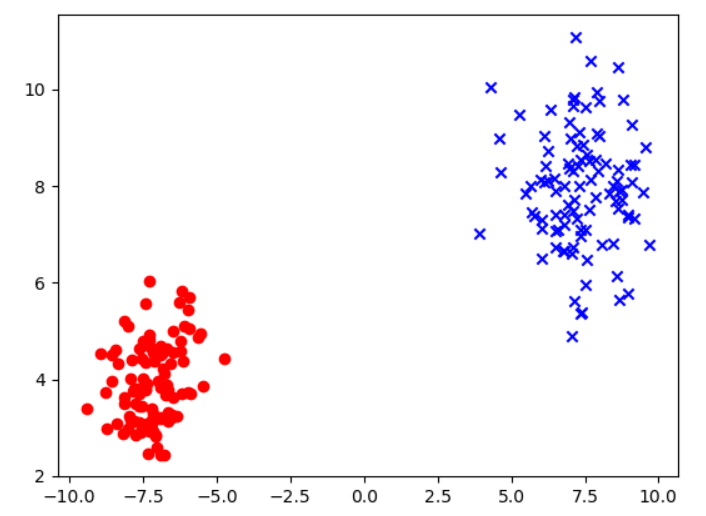
\includegraphics[height=6cm]{images/f000027}
\end{figure}
我们首先来定义逻辑回归模型类:
\lstset{language=PYTHON, caption={逻辑回归模型类(app/pytorch/book/chp003/e1/logistic\_regression\_model.py)}, label={lcrn-logistic-regression-model}}
\begin{lstlisting}
import torch
from torch.autograd import Variable
import torch.nn.functional as F

class LogisticRegressionModel(torch.nn.Module):
    def __init__(self):
        super(LogisticRegressionModel, self).__init__()
        self.l1 = torch.nn.Linear(2, 1)

    def get_weight(self):
        return self.l1.weight

    def get_bias(self):
        return self.l1.bias

    def forward(self, x):
        y_hat = F.sigmoid(self.l1(x))
        return y_hat
\end{lstlisting}
在上面的代码中,我们的网络由一个线性层组成,激活函数为Sigmoid函数。\newline
接下来我们来看模型的训练过程,如下所示:
\lstset{language=PYTHON, caption={二分类逻辑回归训练(app/pytorch/book/chp003/e1/logistic\_regression\_app.py)}, label={lcrn-logistic-regression-train-model}}
\begin{lstlisting}
class LogisticRegressionApp(object):
    def __init__(self):
        self.name = ''

    def run(self):
        print('二分类逻辑回归问题')
        X_train, y_train = self.load_dataset()
        model = LogisticRegressionModel()
        criterion = torch.nn.BCELoss(size_average=True)
        optimizer = torch.optim.SGD(model.parameters(), lr=0.01)
        #optimizer = torch.optim.Adam(model.parameters(), lr=0.01)
        for epoch in range(1000):
            y_hat = model(X_train)
            loss = criterion(y_hat, y_train)
            print('{0}: {1}'.format(epoch, loss.data.item()))
            optimizer.zero_grad()
            loss.backward()
            optimizer.step()
        print(model.parameters)
        w = model.get_weight().data.numpy()
        print('weight:{0}; {1}'.format(w.shape, w))
        b = model.get_bias().data.numpy()
        print('bias:{0}; {1}'.format(b.shape, b))
        # 学习后曲线
        x0 = np.linspace(-1.0, 0.0, 100)
        y0 = -w[0][0]/w[0][1]*x0 - b[0]/w[0][1]*1.14
        plt.plot(x0, y0, '-b')

        x1 = Variable(torch.tensor([[3.31, 0.21]]))
        y1_hat = model.forward(x1).data[0][0]
        print('y={0}'.format(y1_hat))
        plt.show()
\end{lstlisting}
代码解读如下所示:
\begin{itemize}
\item 第7行:载入上一节所介绍的数据集;
\item 第8行:创建逻辑回归模型;
\item 第9行:采用交叉熵代价函数;
\item 第10行:采用随机梯度下降算法来做优化器;
\item 第12行:循环执行13$\sim$18行1000次;
\item 第13行:调用模型前向传播过程求出网络输出;
\item 第14行:计算出代价函数的值;
\item 第15行:打印训练进展情况;
\item 第16行:清空网络参数的微分值缓存;
\item 第17行:利用PyTorch的自动微分求出对网络参数的微分值;
\item 第18行:调用随机梯度下降优化器调整网络参数;
\item 第20行:将连接权值$\boldsymbol{w}$变为numpy数组;
\item 第22行:将偏置值$b$变为numpy数组;
\item 第25$\sim$27行:绘制学习到的分割超平面(直线);
\item 第29行:生成一个测试样本;
\item 第30行:调用模型前向传播过程求出网络输出;
\item 第31行:我们可以看出网络输出为0.9548038840293884,我们可以非常肯定的是该点属于第2类(右上方类别);
\end{itemize}
运行结果如下所示:\begin{figure}[H]
	\caption{逻辑回归二分类学习结果(参数值)图}
	\label{f000029}
	\centering
	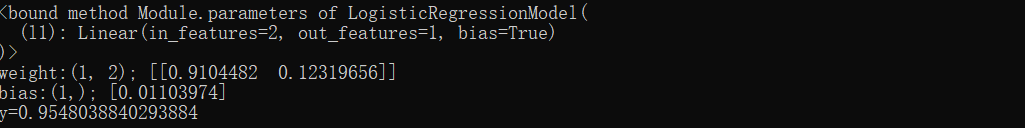
\includegraphics[width=15cm]{images/f000029}
\end{figure}
由上图可以看出,参数值为:$w_{1}=0.9104482$,$w_{2}=0.12319656$,$b=0.01103974$,其分割超平面方程为:$w_{1}x_{1}+w_{2}x_{2} + b=0$,可以将其解析为直线方程:$x_{2}=-\frac{w_{1}}{w_{2}}x_{1} + \frac{b}{w_{2}}$,如下图所示:
\begin{figure}[H]
	\caption{逻辑回归二分类学习结果图}
	\label{f000028}
	\centering
	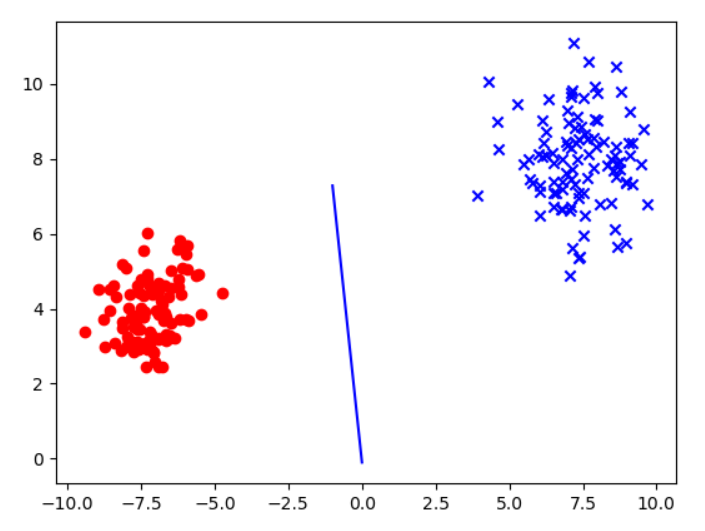
\includegraphics[height=6cm]{images/f000028}
\end{figure}
如上图所示,我们的模型可以正确区分这两个类别,实际上就是在图中找出中间的直线,将样本点划分为两类。

\subsection{softmax回归应用}
\subsubsection{载入MNIST数据集}
MNIST是Mixed National Institute of Standards and Technology的简称,是国际公认的大型手写数字识别数据集,是机器学习算法验证的标准数据集,其地位有点像生物学研究中的大肠杆菌,可以方便地用于各种机器学习算法间性能的比较。实际上,MNIST每年都会组织算法竞赛,以检验各种算法的有效性。\newline
MNIST数据集由纽约大学Yann LeCun教授整理推出,每个手写数字图片的大小均为28$\times$28,黑底白字,并且位于图片中央,共有60000个训练样本集,10000个测试样本集,其中测试样本集是不公开的。\newline
MNIST手写数字图片如下图所示:
\begin{figure}[H]
	\caption{MNIST手写数字识别图片示例}
	\label{f000030}
	\centering
	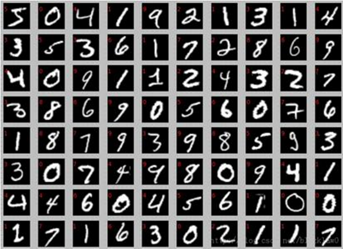
\includegraphics[height=10cm]{images/f000030}
\end{figure}
因为MNIST数据集在国外网站上,通过sklearn.datasets.ftech\_openml下载数据集会有很慢,有时会下载不下来。因此我们采取直接从网站下载别人整理好的CSV格式的文件,然后载入该CSV文件,程序如下所示:
\lstset{language=PYTHON, caption={通过预先下载的CSV文件载入MNIST数据集(app.pytorch.book.chp003.e2.logistic\_regression\_app.py)}, label={lcrn-load-mnist-from-csv}}
\begin{lstlisting}
from __future__ import print_function
import csv
import numpy as np
import matplotlib.pyplot as plt
from mpl_toolkits.mplot3d import Axes3D
import sklearn.datasets as skds
#
from util.npai_ds import NpaiDs
from util.npai_stats import NpaiStats
from ann.ml.logistic_regression import LogisticRegression
from util.npai_plot import NpaiPlot

classMlpApp(object):
    def __init__(self):
        self.name = 'app.ml.Mlp'

    def test_load_mnist_ds(self):
        X, y = self.load_mnist_ds()


    def load_dataset(self):
        # CSV文件下载链接:https://www.openml.org/d/554
        # 从网络上获取数据集:X, y = skds.fetch_openml('mnist_784', version=1, return_X_y=True)
        with open('E:/alearn/dl/npai/data/mnist_784.csv', newline='', encoding='UTF-8') as fd:
            rows = csv.reader(fd, delimiter=',', quotechar='|')
            X0 = None
            y0 = None
            next(rows)
            cnt = 0
            rst = 0
            amount = 1000 # 每1000条记录保存一次
            X = None
            y = None
            for row in rows:
                x = np.array(row[:784], dtype=np.float)
                x /= 255.0
                y_ = np.array(row[784:])
                if None is X:
                    X = np.array([x])
                    y = np.zeros((1, 10))
                    y[cnt, int(y_[0])] = 1
                else:
                    X = np.append(X, x.reshape(1, 784), axis=0)
                    yi = np.zeros((1, 10))
                    yi[0, int(y_[0])] = 1
                    y = np.append(y, yi.reshape(1, 10), axis=0)
                if cnt % amount == 0 and cnt > 0:
                    if None is X0:
                        X0 = X
                        y0 = y
                    else:
                        X0 = np.append(X0, X, axis=0)
                        y0 = np.append(y0, y, axis=0)
                    X = None
                    y = None
                    cnt = 0
                    rst += amount
                    print('处理完{0}记录'.format(rst))
                else:
                    cnt += 1
            idx = 101
            plt.title('{0}th sample: {1}'.format(idx, np.argmax(y[idx])))
            plt.imshow(X[idx].reshape(28, 28), cmap='gray')
            plt.show()
        return X0, y0
\end{lstlisting}
代码解读如下所示:
\begin{itemize}
\item 第19行:在启动程序中选择运行多分类逻辑回归问题;
\item 第29$\sim$31行:定义由CSV文件载入MNIST数据集方法,大家可以通过链接直接从网站上下载CSV格式文件;
\item 第32行:读入下载的CSV文件;
\item 第33行:读取文件中所有行的集合;
\item 第34、35行:定义最终需要返回的样本集和标签集,初始值为空;
\item 第36行:忽略CSV文件的第一行表头信息;
\item 第37行:由于我们为了提高CSV文件读取和转换为数据集的效率,我们以amount条记录为单位,先形成这1000条记录的样本集X和标签集y,然后将其添加到最终样本集X0和最终标签集y0的后面,cnt代表这1000条记录的索引号;
\item 第38行:共处理了多少条数据;
\item 第39行:第1000条数据形成样本集X和标签集y,然后添加到最终样本集X0和最终标签集y0的后面;
\item 第40、41行:amount条数据形成的样本集X和标签集y;
\item 第42$\sim$68行:循环处理CSV文件的每一行;
\item 第43行:由该行前784个元素形成样本,即一个$28 \times 28$的黑白图片;
\item 第44行:由于CSV文件中像素值的取值范围是0$\sim$255,除以255可以变为0$\sim$1区间,方便将来利用matplotlib绘制图形;
\item 第45行:由该行第785个元素形成标签,其值为0$\sim$9的数字,代表该行样本对应的数字,我们在后面将会将该值变为10维的one-hot向量形式来表式;
\item 第46$\sim$49行:如果amount条记录形成的样本集X和标签集y为空,则生成只含有当前样本的样本集X和只含有当前标签的标签集y,对于标签处理,我们先成一个全为零的10维向量,然后根据标签数值,将one-hot向量对应位置的值变为1;
\item 第50$\sim$54行:如果amount条记录形成的样本集X和标签集y不为空,则将当前样本添加到样本集X后面,先成一个全为零的10维向量,然后根据标签数值,将one-hot向量对应位置的值变为1,然后将此标签添加到标签集y的后面;
\item 第55$\sim$66行:如果正好处理了amount条CSV文件中的数据,进行如下处理:
	\begin{itemize}
	\item 第56$\sim$58行:如果最终样本集为空,则最终样本集等于当前样本集,最终标签集等于当前标签集;
	\item 第59$\sim$61行:如果最终样本集不为空,则将当前样本集添加到最终样本集后面,当前标签集添加到最终标签集后面;
	\end{itemize}
\item 第62、63行:将amount条数据对应的样本集X和标签集y置为空;
\item 第64行:amount对应的样本集索引号置为0;
\item 第65行:更新处理完成的总记录数;
\item 第67、68行:如果没处理完amount条CSV文件中数据,增加amount样本集的索引号;
\item 第69行:返回最终样本集X0和最终标签集y0;
\end{itemize}
下面我们来看可视化MNIST数据集:
\begin{itemize}
\item 第21行:定义多分类逻辑回归算法运行程序;
\item 第22行:调用load\_mnist\_ds方法获取样本集X和标签集y;
\item 第23行:指定要显示样本的索引号;
\item 第24行:将样本索引号和样本最终代表的数字作为图片标题,np.argmax可以求出数组中最大元素的索引号;
\item 第25行:将样本数据重新组织为$28\times28$的黑白图像格式,并利用matplotlib进行绘制,如下所示:
\begin{figure}[H]
	\caption{MNIST手写数字识别单位样本示例}
	\label{f000031}
	\centering
	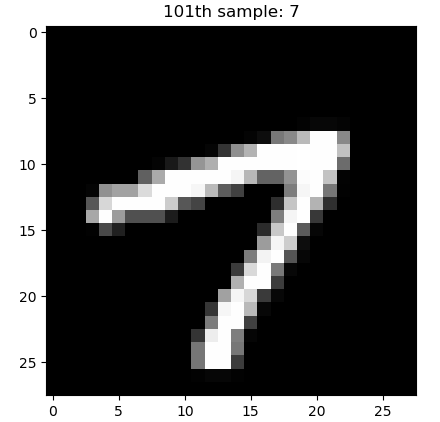
\includegraphics[height=10cm]{images/f000031}
\end{figure}
\end{itemize}
\subsubsection{MNIST数据集可视化}
由于手写数字识别数据集MNIST为$28 \times 28$的黑白图像,所以每个样本是784维,而我们只能直观的看到二维样本的情形。为了能够直观的显示MNIST数据集,我们使用t-SNE算法,将其变为二维形式进行展示。代码如下所示(app/pytorch/book/chp003/e2/logistic\_regression\_app.py):
\lstset{language=PYTHON, caption={t-sne可视化MNIST数据集}, label={lcrn-mnist-tsne}}
\begin{lstlisting}
class MlpApp(object):
    def __init__(self):
        self.name = 'ann.ml.MlpApp'
    
    def show_mnist_in_tsne(self):
        X, y_ = self.load_mnist_ds()
        y = np.argmax(y_, axis=1)
        row_embedded = skmd.TSNE(n_components=2).fit_transform(X)
        pos = pd.DataFrame(row_embedded, columns=['X', 'Y'])
        pos['species'] = y
        ax = pos[pos['species']==0].plot(kind='scatter', x='X', y='Y', color='blue', label='0')
        pos[pos['species']==1].plot(kind='scatter', x='X', y='Y', color='red', label='1', ax=ax)
        pos[pos['species']==2].plot(kind='scatter', x='X', y='Y', color='green', label='2', ax=ax)
        pos[pos['species']==3].plot(kind='scatter', x='X', y='Y', color='yellow', label='3', ax=ax)
        pos[pos['species']==4].plot(kind='scatter', x='X', y='Y', color='brown', label='4', ax=ax)
        pos[pos['species']==5].plot(kind='scatter', x='X', y='Y', color='orange', label='5', ax=ax)
        pos[pos['species']==6].plot(kind='scatter', x='X', y='Y', color='black', label='6', ax=ax)
        pos[pos['species']==7].plot(kind='scatter', x='X', y='Y', color='pink', label='7', ax=ax)
        pos[pos['species']==8].plot(kind='scatter', x='X', y='Y', color='purple', label='8', ax=ax)
        pos[pos['species']==9].plot(kind='scatter', x='X', y='Y', color='cyan', label='9', ax=ax)
        plt.show()
\end{lstlisting}
代码解读如下所示:
\begin{itemize}
\item 第5行:定义t-sne算法显示MNIST数据集方法;
\item 第6行:读入MNIST数据集,$X \in R^{m \times 784}$为样本集,每一行为一个图片,$\boldsymbol{y} \in R^{10}$为one-hot向量,不为0的索引值代表对应的数据;
\item 第7行:将原来的以one-hot向量形式的标签集,变为索引号形式;
\item 第8行:调用sklearn.manifold.TSNE方法进行降维处理;
\item 第9行:将其变为两列的pandas.DataFrame;
\item 第10行:将标签作为DataFrame的第三列;
\item 第11行:将标签为0的记录,以蓝色散点图形式绘制到图片中;
\item 第12$\sim$19行:将类别为1到9的样本,以不同颜色散点图形大绘制到图片中;
\item 第20行:显示图片;
\end{itemize}
t-SNE图片如下所示:
\begin{figure}[H]
	\caption{MNIST数据集t-SNE图}
	\label{f000032}
	\centering
	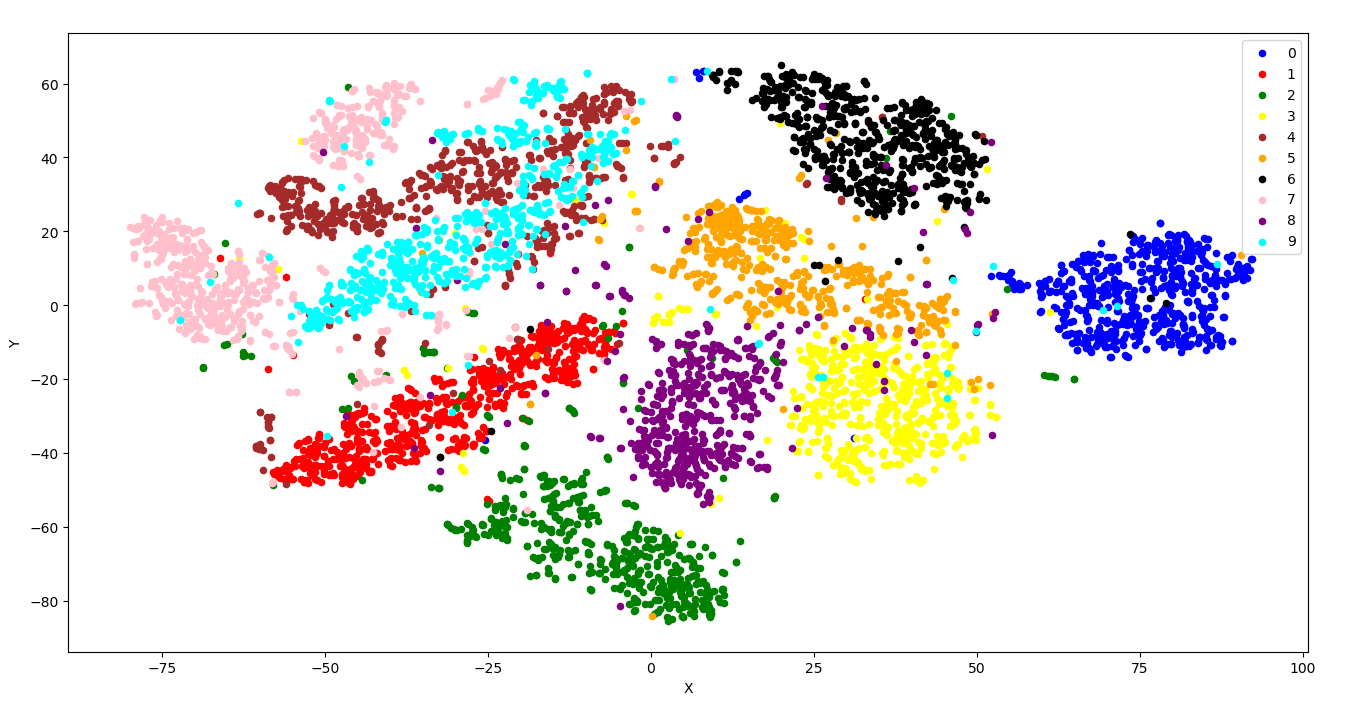
\includegraphics[height=8cm]{images/f000032}
\end{figure}
由上图可以看出,通过选择合理的特征,我们还是可以将手写数字区分开的。
\subsubsection{代码实现}
在这一部分,我们将来看怎样用PyTorch实现softmax回归(即多分类逻辑回归),为了代码的完整性,我们在这里列出了完整的类代码,我们先来看多分类逻辑回归模型类,如下所示(app/pytorch/book/chp003/e2/logistic\_regression\_model.py):
\lstset{language=PYTHON, caption={softmax回归模型类}, label={lcrn-softmax-regression-model}}
\begin{lstlisting}
class LogisticRegressionModel(torch.nn.Module):
    def __init__(self):
        super(LogisticRegressionModel, self).__init__()
        self.l1 = torch.nn.Linear(784, 10)

    def get_weight(self):
        return self.l1.weight

    def get_bias(self):
        return self.l1.bias

    def forward(self, x):
        return F.softmax(self.l1(x))
\end{lstlisting}
上面的代码与二分类逻辑回归模型类基本相同,所不同的是:
\begin{itemize}
\item 第4行:定义线性模型时,输出信号维度为10,代表10个数字现现的概率;
\item 第13行:将输出层激活函数由Sigmoid函数变为softmax函数;
\end{itemize}
我们接下来看多分类逻辑回归应用类,如下所示(app/pytorch/book/chp003/e2/logistic\_regression\_app.py):
\lstset{language=PYTHON, caption={softmax回归代码实现}, label={lcrn-softmax-regression-app}}
\begin{lstlisting}
class LogisticRegressionApp(object):
    def __init__(self):
        self.name = ''
        plt.rcParams['font.sans-serif'] = ['SimHei']
        plt.rcParams['axes.unicode_minus'] = False

    def run(self):
        print('softmax回归MNIST应用')
        X_train, y_train = self.load_dataset()
        epochs = 1000
        model = LogisticRegressionModel()
        criterion = torch.nn.BCELoss(size_average=True)
        optimizer = torch.optim.SGD(model.parameters(), lr=0.01)
        #optimizer = torch.optim.Adam(model.parameters(), lr=0.01)
        for epoch in range(epochs):
            y_hat = model(X_train)
            loss = criterion(y_hat, y_train)
            print('{0}: {1}'.format(epoch, loss.data.item()))
            optimizer.zero_grad()
            loss.backward()
            optimizer.step()
        w = model.get_weight().data.numpy()
        print('weight:{0}; {1}'.format(w.shape, w))
        b = model.get_bias().data.numpy()
        print('bias:{0}; {1}'.format(b.shape, b))
        # 测试模型
        idx = 118
        Xt = X_train[idx:idx+1, :]
        yt = y_train[idx:idx+1, :]
        yt_hat = model(Xt)
        print('Xt:{0}; yt:{1}; yt_hat:{2}'.format(Xt.shape, yt.shape, yt_hat.shape))
        r = torch.argmax(yt)
        r_hat = torch.argmax(yt_hat)
        print('r:{0}; r_hat:{1}'.format(r, r_hat))
        plt.title('第{0}张图预测结果: {1}'.format(idx+1, r_hat))
        X_raw = Xt[0].numpy().reshape(28, 28)
        plt.imshow(X_raw, cmap='gray')
        plt.show()

    def load_dataset(self):
        # CSV文件下载链接:https://www.openml.org/d/554
        # 从网络上获取数据集:X, y = skds.fetch_openml('mnist_784', version=1, return_X_y=True)
        with open('E:/alearn/dl/npai/data/mnist_784.csv', newline='', encoding='UTF-8') as fd:
            rows = csv.reader(fd, delimiter=',', quotechar='|')
            X0 = None
            y0 = None
            next(rows)
            cnt = 0
            rst = 0
            amount = 1000 # 每1000条记录保存一次
            X = None
            y = None
            for row in rows:
                x = np.array(row[:784], dtype=np.float)
                x /= 255.0
                y_ = np.array(row[784:])
                if None is X:
                    X = np.array([x])
                    y = np.zeros((1, 10))
                    y[cnt, int(y_[0])] = 1
                else:
                    X = np.append(X, x.reshape(1, 784), axis=0)
                    yi = np.zeros((1, 10))
                    yi[0, int(y_[0])] = 1
                    y = np.append(y, yi.reshape(1, 10), axis=0)
                if cnt % amount == 0 and cnt > 0:
                    if None is X0:
                        X0 = X
                        y0 = y
                    else:
                        X0 = np.append(X0, X, axis=0)
                        y0 = np.append(y0, y, axis=0)
                    X = None
                    y = None
                    cnt = 0
                    rst += amount
                    print('处理完{0}记录'.format(rst))
                else:
                    cnt += 1
            #self.draw_dataset(X0, y0)
            print('X0:{0} vs {2}; y0:{1} vs {3}'.format(X0.shape, y0.shape, X0.dtype, y0.dtype))
            X0 = np.array(X0, dtype=np.float32)
            y0 = np.array(y0, dtype=np.float32)
        return Variable(torch.from_numpy(X0)), Variable(torch.from_numpy(y0))
\end{lstlisting}
代码解读如下所示:
\begin{itemize}
\item 第行:;
\item 第行:;
\item 第行:;
\item 第行:;
\item 第行:;
\end{itemize}
运行结果如下所示:
\begin{figure}[H]
	\caption{运行结果后台输出}
	\label{f000033}
	\centering
	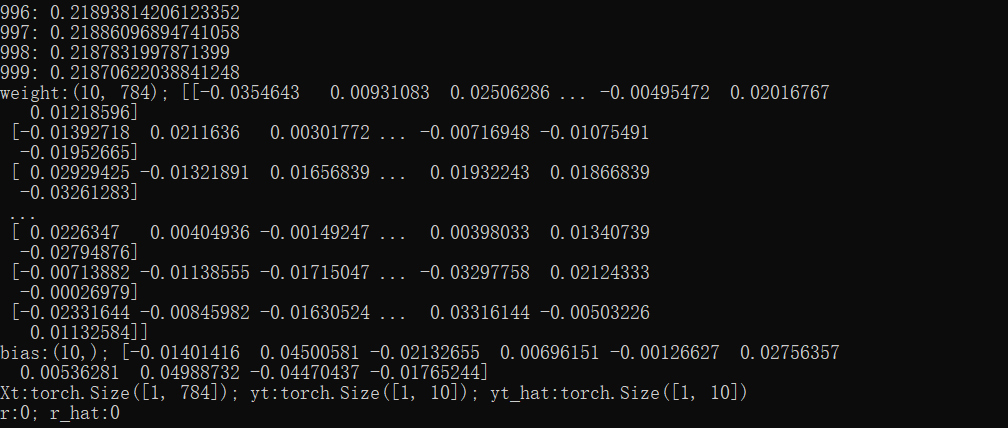
\includegraphics[width=15cm]{images/f000033}
\end{figure}
\begin{figure}[H]
	\caption{运行结果示意图}
	\label{f000034}
	\centering
	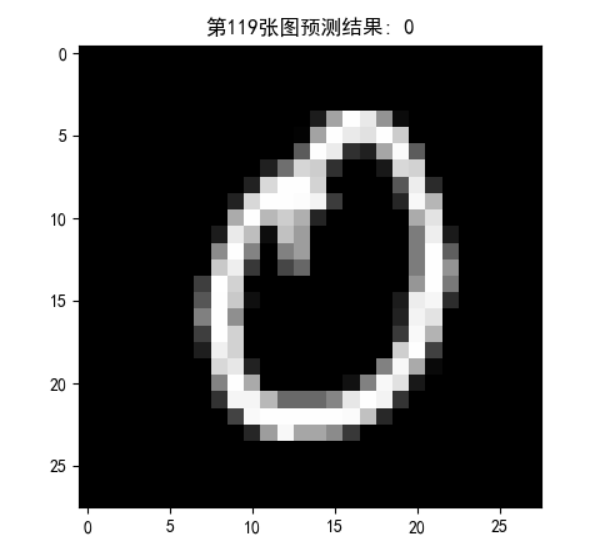
\includegraphics[height=8cm]{images/f000034}
\end{figure}
由上图可见,我们模型还是可以预测出正确结果的。需要注意的是,我们这里作为示例,使用的是刚训练过的训练数据集中的样本,实际上这样验证模型的精度是有严重问题的。实际上,我们应该用训练数据集来训练模型,从独立同分布(IID)中采样的验证样本集上精度变化情况,决定何时停止训练以及选择哪些超参数,当模型训练结束后,再运行测试数据集,得到在测试数据集上的精度,作为模型在实际应用中近似的精度。
\subsection{总结}
在本章中,我们详细讲解了逻辑回归算法的数学原理,包括通用学习模型和牛顿法,重点讲解了二分类问题和多分类问题,对于二分类问题,我们讲解了自己生成的人工数据的解决方案,对于多分类问题,我们使用手写数字识别MNIST数据集,向大家演示了应用方法。但是大家可能注意到,在本章的例子中,我们并没有采用训练数据集、验证数据集和测试数据集,也没有考虑过拟合(Over-Fitting)问题,这些问题我们将在下一章多层感知器模型中进行讲解,作为练习,大家可以在阅读完下一章后,将本章的程序改造为使用验证数据集、测试数据集,使用Early Stopping、Dropout等调整手段保证不过拟合(Over-Fitting)的实用算法。


\newpage
\maketitle
\begin{center}
\Large \textbf{第5章 多层感知器} \quad \textbf{}
\end{center}
\begin{abstract}
在本章中我们将详细讲解多层感知器(MLP)模型,本章分为三大部分:第一部分:我们将以一个简单的例子为例,讲解怎样使用Numpy来做多层感知器(MLP)模型,重点在于讲解多层感知器模型的数学原理;第二部分我们将以PyTorch的典型方式实现多层感知器模型;第三部分是使用PyTorch底层技术来实现多层感知器(MLP)模型。
\end{abstract}
\section{多层感知器(MLP)概述}
多层感知器(MLP)模型是最老的一类神经网络模型,以前人们通常认为多层感知器(MLP)模型的能力有限,而且根据万能逼近理论,只有一层的神经网络,只要中间层有足够多的节点,就可以拟合任意复杂的函数。所以很长时间以来,研究人员通常认为浅而宽的神经网络是最好的神经网络结构,没有必要采用深层神经网络。但是在2006年,深度学习之父Hinton通过预训练方式,使得基于多层感知器(MLP)模型的深度信念网络(DBN)取得重大成功,成为当代深度学习技术崛起的开端。此后随着Web2.0的发展,有了越来越大的训练数据集,通过利用GPU,使算力提到上百倍的提升。人们发现,多层感知器(MLP)模型具有巨大的应用潜力,是功能最为强大的神经网络模型。其他在深度学习领域大获成功的模型,利如卷积神经网络(CNN)、递归神经网络(RNN)都可以视为多层感知器(MLP)模型的特例。\newline
通过研究多层感知器(MLP)的发展历史,其由上世纪90年代被打入冷宫,到今天在深度学习时代大行其道,在这中间有三项关键的推动因素:第一项是更加适合的代价函数,在此之前,人们普遍采用平均平方误差(MSE)来衡量,神经元激活函数通常采用Sigmoid函数,由于Sigmoid函数的特点,在偏差值较大时,反而是其曲线非常平坦的区域,所以学习速度会非常慢,所以以前的深层网络非常难以训练,到近代之后,人们逐渐采用交叉熵(CrossEntropy)作为代价函数,极大缓解了深层网络学习缓慢的问题;第二项是在原来的深层网络中,人们在隐藏层也采用Sigmoid函数,由于Sigmoid函数的特点,在输出值较大或较小时,其微分都非常接近于零,因此学习速率非常低,这种现象在深层网络中尤其明显,在当代,人们采用ReLU函数及其变体LickyReLU、SeLU、ELU等激活函数作为隐藏层神经元的激活函数,这些函数的特点是当神经元输入小于某个阈值时,神经元处于非激活状态,其微分值为零,当超过该阈值时,其微分值为某个正数,与输入的信号大小无关,正是由于这一特性,成功的解决了多层神经网络训练慢的问题;第三项与算法改进的关系不大,但是可能是最重要的原因,就是随着Web2.0的兴起,人们掌握了越来越大的数据集,例如ImageNet数据集就有1200万张图片,而且从2012年之后,GPU在深度学习中的应用成为常态,与CPU相比,可以提高几十倍的计算效率,正是由于这些技术上的进步,使得多层感知器(MLP)模型这一古老的模型具有越来越大的应用前景。
\subsection{数学原理}
\subsubsection{前向传播过程}
在本节中,我们想向大家介绍多层感知器(MLP)模型的表示方式,这同时是各种神经网络的表示基础。\newline
我们假定第$l-1$层具有$N_{l-1}$个神经元,其输出信号为一个向量$\boldsymbol{a}^{l-1}$:
\begin{equation}
\boldsymbol{a}^{l-1}= \begin{bmatrix}
a_{1}^{l-1} \\
a_{2}^{l-1} \\
... \\
a_{N_{l-1}}^{l-1} \\
\end{bmatrix} \in R^{N_{l-1}}
\label{mlp-a-l-1}
\end{equation}
其中第$j$个神经元的输出为$a_{j}^{l-1}$,其上标代表是第$l-1$层,下标代表是第$j$个神经元。
第$l$层有$N_{l}$个神经元,第$l-1$层和第$l$层神经元互相两两全部连接,连接权值$W$为:
\begin{equation}
W^{l}=\begin{bmatrix}
W_{1,1}^{l} & W_{1,2}^{l} & ... & W_{1,N_{l-1}}^{l} \\
W_{1,1}^{l} & W_{1,2}^{l} & ... & W_{1,N_{l-1}}^{l} \\
... & ... & ... & ... \\
W_{N_{l},1}^{l} & W_{N_{l},2}^{l} & ... & W_{N_{l},N_{l-1}}^{l} \\
\end{bmatrix}
\label{mlp-w-l-1-l}
\end{equation}
第$l-1$层第$j$个神经元指向第$l$层第$i$个神经元的连接权值为$W_{i,j}^{l}$。\newline
第$l$层的输入用向量$\boldsymbol{z}^{l}$表示:
\begin{equation}
\begin{aligned}
\boldsymbol{z}^{l} = W^{l} \cdot \boldsymbol{a}^{l-1} + \boldsymbol{b} \\
z_{i}^{l} = W_{i,:}^{l} \cdot \boldsymbol{a}^{l-1} + b_{i} \\
= W_{i,1} a_{1}^{l-1} + W_{i,2} a_{2}^{l-1} + ... + W_{i,N_{l-1}} a_{N_{l-1}}^{l-1} \\
= \sum_{j=1}^{N_{l-1}} W_{i,j}^{l} \cdot a_{j}^{l-1} + b_{i}
\end{aligned}
\label{mlp-z-l-def}
\end{equation}
我们假设第$l$层的激活函数为$f(x)$,则第$l$层输出为:
\begin{equation}
\boldsymbol{a}^{l}= f(\boldsymbol{z}^{l})
\label{mlp-a-l-def}
\end{equation}
依次运行上述步骤,即可完成神经网络的前向传播过程,求出输出层的输出。
\subsubsection{神经元激活函数}
\paragraph{sigmoid函数}
在现代深度学习技术复兴之前,sigmoid函数是神经元缺省的激活函数,因为sigmoid的函数在定义域内连续且处处可微,同时可以解释为事件出现的概率,所以成为神经元的缺省激活函数。但是近些年来,人们逐渐意识到,sigmoid函数在其定义域内在值过大或过小时,会出现饱合情况,曲线变得非常平坦,这时求导时值就几乎为零,这使得基于求导的梯度下降法收敛很慢,这种情况在深度网络中尤其严重,会出现梯度消失的问题,在这期间传统的机器学习方法,例如支撑向量机(SVM)却没有这个问题,所以近年来,除了二元分类问题的输出层,长短时记忆网络(LSTN)的门限操作,等比较特殊的情形外,人们已经不再使用sigmoid函数作为神经元的激活函数了,在现代深度学习网络中,缺省的隐藏层激活函数是ReLU函数。ReLU函数是一个分段线性函数,除零点外处处可导,不存在梯度消失问题,所有这些特点使得ReLU成为深度学习网络理想的神经元激活函数。
\subparagraph{定义}
sigmoid函数定义如下所示:
\begin{equation}
\begin{aligned}
\sigma(x)=\frac{1}{1 + e^{-x}}
\end{aligned}
\label{mlp-sigmoid-def}
\end{equation}
我们可以用如下代码绘制sigmoid函数的图形:
\lstset{language=PYTHON, caption={绘制sigmoid函数}, label={mlp-draw-sigmoid}}
\begin{lstlisting}
import numpy as np
import matplotlib.pyplot as plt

def main():
    x = np.linspace(-10, 10, 300)
    y = 1.0 / (1 + np.exp(-x))
    plt.plot(x, y)
    plt.show()

if '__main__' == __name__:
    main()
\end{lstlisting}
上面代码绘制出来的sigmoid函数图形如下所示:
\begin{figure}[H]
	\caption{sigmoid函数}
	\label{f000035}
	\centering
	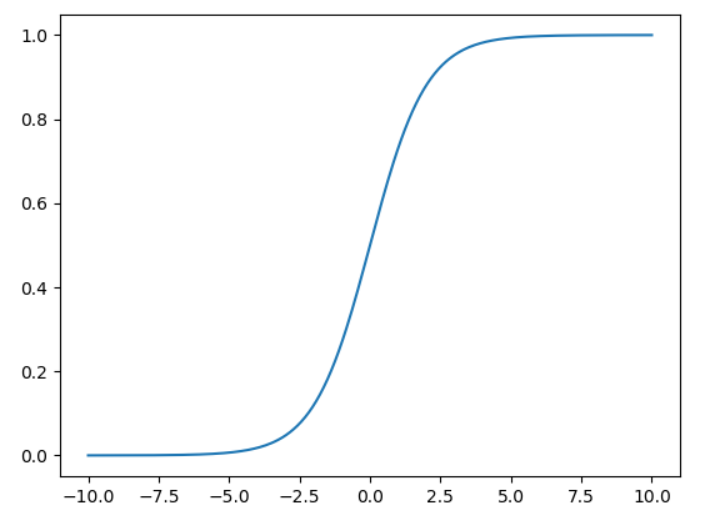
\includegraphics[height=5cm]{images/f000035}
\end{figure}
如图\ref{f000035}所示,当函数自变量x的值大于5或小于-5时,函数曲线就变得非常平坦了,这时导数将非常小,几乎接近于零,这时梯度下降算法收敛的速度就会相当慢,为了解决这一问题,研究人员提出了ReLU函数作为隐藏层神经元的激活函数,并逐渐成为深度学习网络中主流技术。我们将在本节稍后时间给大家讲解ReLU函数。
\subparagraph{导数}
对于一个可导的函数$f(x)$,我们将其在$x_0$点的导数定义为:
\begin{equation}
\begin{aligned}
\frac{dy}{dx}=lim_{x \to x_0} \frac{f(x)-f(x_0)}{x-x_0}
\end{aligned}
\label{mlp-sigmoid-devirative-math-def}
\end{equation}
这是导数的定义,我们验证求导函数是否正确时,就是用这种方式来进行正确性检验的。但是在深度学习中,我们不使用这个定义来求导,因为这种数值计算方式不仅运算量大,而且精度低,当前业界的主流求导技术是自动微分技术,这个技术我们会在本节最后给大家做一个简单的介绍。\newline
回到求导问题上来,我们一般应用解析法来求导,这非常类似于我在学高等数学时的手工求导公式。高等数学中求导公式有很多,但是对于sigmoid函数求导来说,只需要用到如下两个公式:
\begin{equation}
\begin{aligned}
(e^x)'=e^x
\end{aligned}
\label{mlp-devirative-formula-1}
\end{equation}
\begin{equation}
\begin{aligned}
\big( \frac{u}{v} \big)' = \frac{u'\cdot v-u \cdot v'}{v^2} \quad v \ne 0
\end{aligned}
\label{mlp-devirative-formula-2}
\end{equation}
对于sigmoid函数而言,分母$u=1$,式\ref{mlp-devirative-formula-2}就可以简化为:
\begin{equation}
\begin{aligned}
\big( \frac{1}{v} \big)' = \frac{-v'}{v^2} \quad v \ne 0
\end{aligned}
\label{mlp-devirative-formula-3}
\end{equation}
根据以上公式,sigmoid导数为:
\begin{equation}
\begin{aligned}
\sigma(x)'=\frac{-(1+e^{-x})'}{(1+e^{-x})^2}=-\frac{-e^{-x}}{(1+e^{-x})^2}=\frac{e^{-x}}{(1+e^{-x})^2}\\
=\frac{1}{1+e^{-x}} \cdot \frac{e^{-x}}{1+e^{-x}}=\frac{1}{1+e^{-x}} \cdot \big( 1 - \frac{1}{1+e^{-x}} \big)\\
=\sigma(x) \cdot \big( 1- \sigma(x) \big)
\end{aligned}
\label{mlp-sigmoid-devirative-formula}
\end{equation}

\paragraph{ReLU函数}
ReLU函数的定义为:
\begin{equation}
\begin{aligned}
g(\boldsymbol{z})=\max\{ 0, z \}
\end{aligned}
\label{mlp-relu-def}
\end{equation}
用我们常用的数学语言来描述,ReLU就是一个分段函数:
\begin{equation}
\begin{aligned}
g(\boldsymbol{z})=
\begin{cases}
0, \quad z < 0 \\
z, \quad z \ge 0
\end{cases}
\end{aligned}
\label{mlp-relu-def-1}
\end{equation}
大家可以看到,在$z < 0$时,函数的导数为零,当$z>0$时,函数的导数为常数1,不存在饱合问题,同时具有线性函数的简洁性,降低了深度神经网络的训练难度。
可以通过如下代码绘制ReLU函数:
\lstset{language=PYTHON, caption={绘制ReLU函数}, label={mlp-code-draw-relu}}
\begin{lstlisting}
import numpy as np
import matplotlib.pyplot as plt

def relu(x):
    s = np.where(x<0, 0, x)
    return s


def relu_grad(s):
    ds = np.where(s<0, 0, 1)
    return ds

def main():
    x = np.linspace(-10, 10, 200)
    y = relu(x)
    plt.plot(x, y)
    plt.show()

if '__main__' == __name__:
    main()
\end{lstlisting}
ReLU函数的图形如下所示:
\begin{figure}[H]
	\caption{ReLU函数图像}
	\label{f000036}
	\centering
	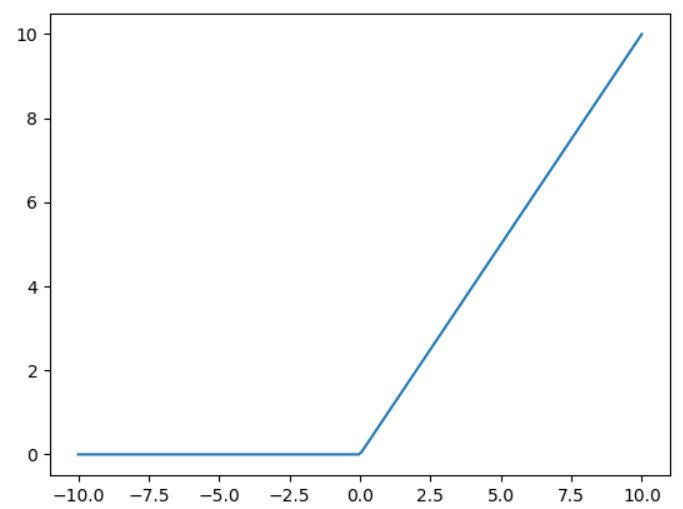
\includegraphics[height=3cm]{images/f000036}
\end{figure}
ReLU函数与Sigmoid函数正好相反,虽然在$x=0$时不可微,但是其他处均可微,现代深度学习理论认为,只要函数绝大多数地方可微就可以了。另外,ReLU函数也不存在饱合性,当$x>0$时,其微分值始终为1,可以加快梯度下降算法的收敛速度。同时,ReLU函数很好地模拟了生物神经元刺激在一定阈值下不反应,达到这个阈值后起反应,但是和刺激强度无关的特性。正是由于采用了ReLU函数,才使得现代的深度学习网络取得成功。
\subsubsection{深度学习中的微分运算}
深度学习当中,函数微分是一项非常重要的任务。关于计算机实现函数微分,总结起来有以下三种方式:第一种直接按导数定义的数值计算方法,这种方法的优点是简单,但是缺点是计算量大并且精度低,通常只用于验证其他微分方法的正确性;第二种方法是解析法,就是像我们在上一节对sigmoid函数那样,手工求出函数微分的表达式,这种方式的精度高,但是很多函数不容易解出微分的表达式,同时利用隐函数表示的函数,也很难求出微分表达式;第三种方法就是未来可能会流行起来的自动微分方法,深度学习三巨头之一的Yann LeCun在去年所说的“深度学习已死,可微编程永生”就是指的这种方法。这一部分内容可以参考我的博客\cite{r000004}。\newline
在这一节中,我们将以一个简单的逻辑回归模型,来带领大家掌握三种主流的求微分的方式,同时向大介绍自动微分技术。去年深度学习三巨头之一Yann LeCun曾经说:“深度学习已死,可微编程永生”,他说的可微编程就是自动微分技术,所以有必要介绍一下这个最新技术。\newline
在逻辑回归模型中,我们的输入为向量$\boldsymbol{x}$,与权值向量$\boldsymbol{w}$相乘,再加上偏置值b,再将得到的结果取Sigmoid函数,最后就得到了一个0$\sim$1的判别结果,如下所示:
\begin{equation}
\begin{aligned}
\hat{y}=\frac{1}{1+e^{-(\boldsymbol{w}\cdot \boldsymbol{x} + b)}}
\end{aligned}
\label{mlp-lcrn-output-forward}
\end{equation}
\paragraph{数值法}
数值法求微分就是利用导数的定义来求微分值,根据高等数学导数的定义:
\begin{equation}
\begin{aligned}
f(x)'=\lim_{x \to x_0}\frac{f(x)-f(x_0)}{x-x_0}
\end{aligned}
\label{mlp-math-devirative-def}
\end{equation}
在实际中为了有更好的效果,我们通常采用这种方式来计算微分:
\begin{equation}
\begin{aligned}
f(x)'=\lim_{h \to 0}\frac{f(x+h) - f(x-h)}{2 \cdot h}
\end{aligned}
\label{mlp-math-devirative-def-fine}
\end{equation}
\paragraph{公式法求微分}
公式法就是根据高等数学公式,求出函数微分的表达式,将数值代入表达式求出微分值。实际上我们在Sigmoid函数一节中,就是用这种方式求的微分。具体求导过程如下所示:
\begin{equation}
\begin{aligned}
\hat{y}=\frac{d(\frac{1}{1+e^{-\boldsymbol{w}^T \cdot \boldsymbol{x}-b}})}{d\boldsymbol{x}}=-\frac{(1+e^{-\boldsymbol{w}^T \cdot \boldsymbol{x}-b})'}{(1+e^{-\boldsymbol{w}^T \cdot \boldsymbol{x}-b})^2}=-\frac{(e^{-\boldsymbol{w}^T \cdot \boldsymbol{x}-b})'}{(1+e^{-\boldsymbol{w}^T \cdot \boldsymbol{x}-b})^2}\\
=-\frac{e^{-\boldsymbol{w}^T \cdot \boldsymbol{x}-b} \cdot (-\boldsymbol{w}^T \cdot \boldsymbol{x}-b)'}{(1+e^{-\boldsymbol{w}^T \cdot \boldsymbol{x}-b})^2}\\
=\frac{e^{-\boldsymbol{w}^T \cdot \boldsymbol{x}-b} }{(1+e^{-\boldsymbol{w}^T \cdot \boldsymbol{x}-b})^2} \cdot \boldsymbol{w} \\
=\frac{1}{1+e^{-\boldsymbol{w}^T \cdot \boldsymbol{x}-b}}\frac{e^{-\boldsymbol{w}^T \cdot \boldsymbol{x}-b} }{1+e^{-\boldsymbol{w}^T \cdot \boldsymbol{x}-b}} \cdot \boldsymbol{w} \\
=\hat{y}(1-\hat{y})\boldsymbol{w}
\end{aligned}
\label{mlp-math-devirative-formula}
\end{equation}

这里用的技巧就是高等数学在复合函数求导中用的换元法,就是把复杂的部分视为一个整体先求导,然后再乘以对这个部分进行求导,这个过程一直进行下去,直到求到自变量时为止。另外,注意这里是对输入信号的微分,而不是我们在深度学习中经常使用的对连接权值的微分,但是这一技术确实是有用的,在生成对抗样本时就是使用这一技术。
\paragraph{计算图法}
计算图是当前深度学习框架所用到的主流技术,可以在计算图上直接运行BP算法,得到网络参数的微分。下面我们就以逻辑回归用到的输出层激活函数为例:
\begin{equation}
\begin{aligned}
y=\frac{1}{1+e^{-(\boldsymbol{w}^T \cdot \boldsymbol{x}+b)}}
\end{aligned}
\label{mlp-sigmoid-def2}
\end{equation}
我们假设我们求不出这个函数的导数,只是将这个函数拆成简单函数的组合,对应的计算图如下所示:
\begin{figure}[H]
	\caption{计算图基本形式}
	\label{f000037}
	\centering
	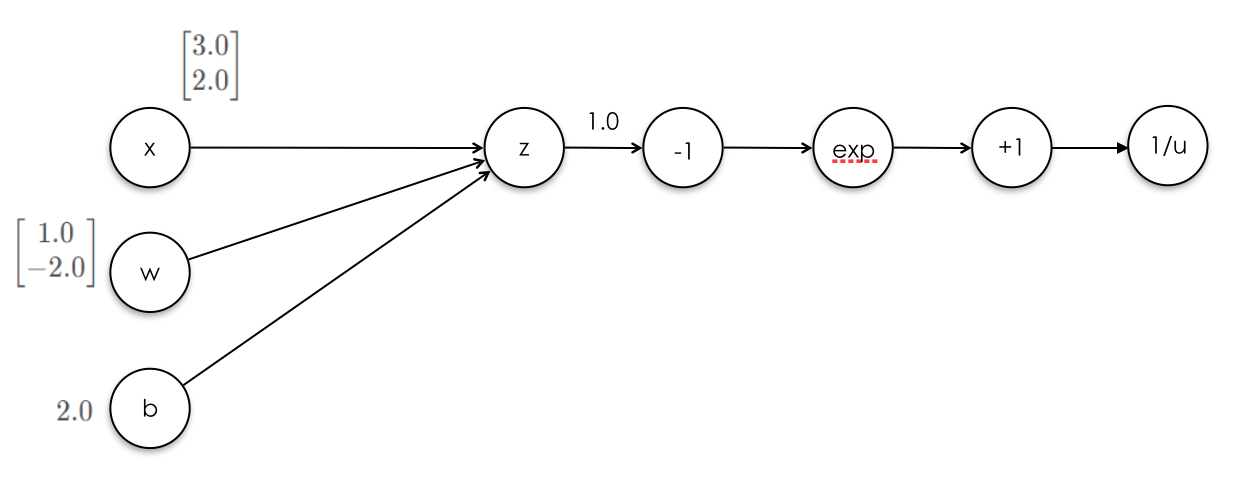
\includegraphics[height=5cm]{images/f000037}
\end{figure}
图中第1个需要计算的节点就是z节点,计算公式为:
\begin{equation}
\begin{aligned}
z=\boldsymbol{w}^T \cdot \boldsymbol{x}+b=\begin{bmatrix}
1.0 \\
-2.0
\end{bmatrix}^T \cdot \begin{bmatrix}
3.0 \\
2.0
\end{bmatrix}+2.0=1.0
\end{aligned}
\label{mlp-sigmoid-cg-1}
\end{equation}
计算出来的值我们写在z节点后,箭头线的上方。\newline
接着我们来算-1这个节点,计算公式如下所示:
\begin{equation}
\begin{aligned}
-u=-1.0
\end{aligned}
\label{mlp-sigmoid-cg-2}
\end{equation}
将计算结果写在-1这个节点右侧箭头线的上方,如下图所示:
\begin{figure}[H]
	\caption{计算图基本形式}
	\label{f000038}
	\centering
	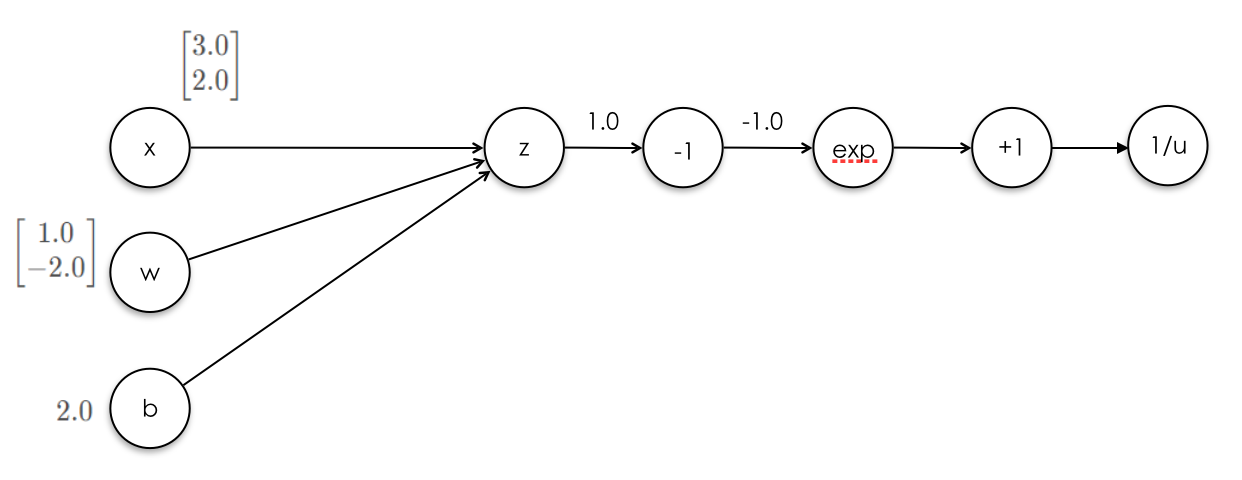
\includegraphics[height=5cm]{images/f000038}
\end{figure}
我们接下来计算exp节点,计算公式如下所示:
\begin{equation}
\begin{aligned}
e^u=e^{-1}=-\frac{1}{2.71828 18284 59}=0.37
\end{aligned}
\label{mlp-sigmoid-cg-3}
\end{equation}
将计算结果写到exp节点右侧箭头线的上方,如下图所示:
\begin{figure}[H]
	\caption{计算图基本形式}
	\label{f000039}
	\centering
	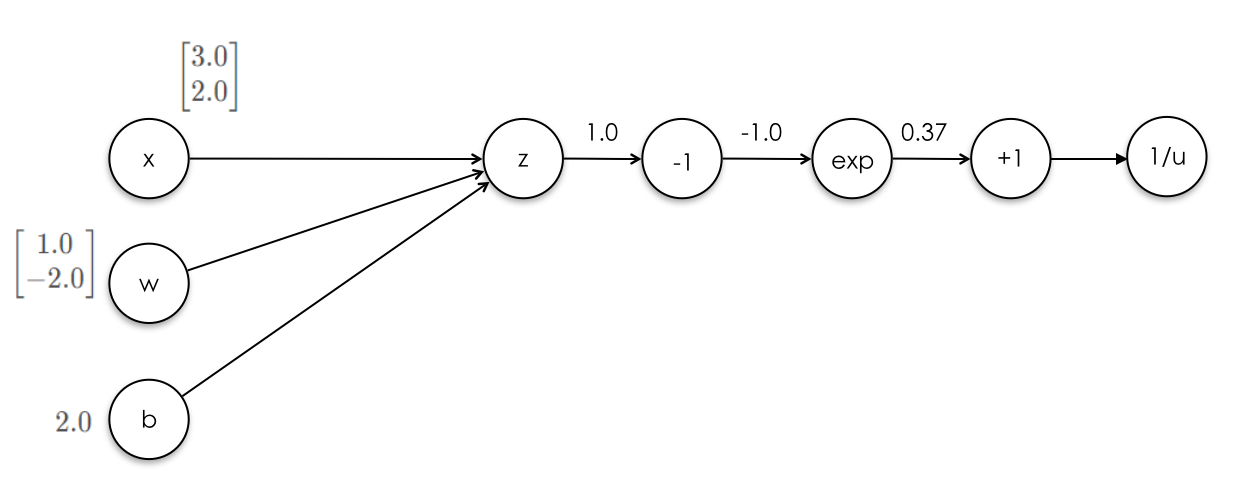
\includegraphics[height=5cm]{images/f000039}
\end{figure}

接下来一步是计算求+1节点,并把计算结果写到右侧箭头线上方,如下图所示:
\begin{figure}[H]
	\caption{计算图基本形式}
	\label{f000040}
	\centering
	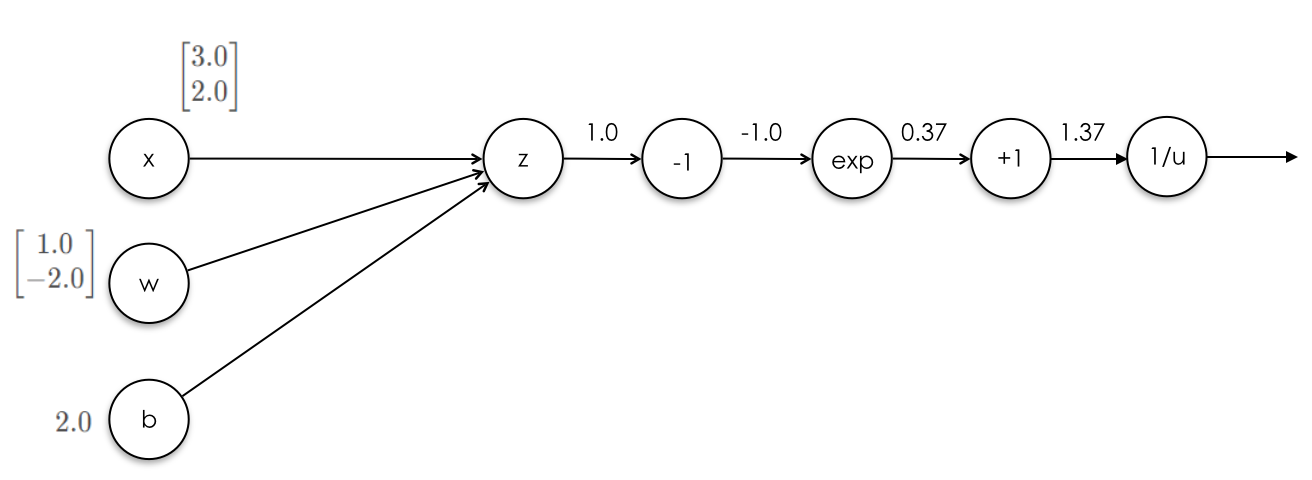
\includegraphics[height=5cm]{images/f000040}
\end{figure}
最后我们计算1/u节点,计算公式如下所示:
\begin{equation}
\begin{aligned}
\frac{1}{u}=\frac{1}{1.37}=0.73
\end{aligned}
\label{mlp-sigmoid-cg-4}
\end{equation}
将求出的结果写到1/u节点的右侧箭头线的上方,如下图所示:
\begin{figure}[H]
	\caption{计算图基本形式}
	\label{f000041}
	\centering
	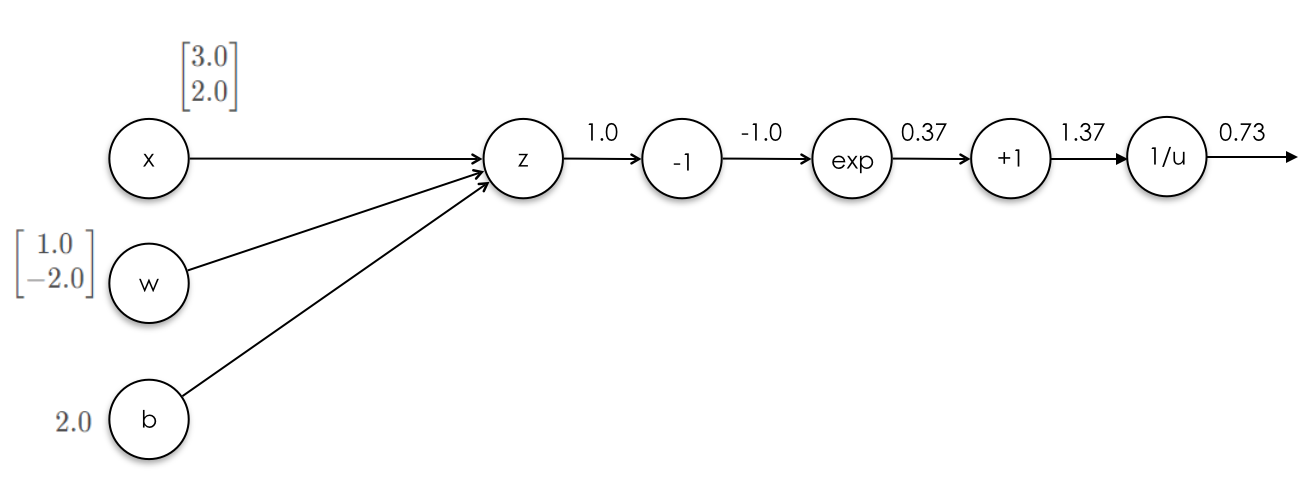
\includegraphics[height=5cm]{images/f000041}
\end{figure}
以上就是信号正向传播的过程。接下来就是反向求微分值的过程。我们第一步是在计算图最后一步,即1/u节点右侧箭头线下方写上1,
代表输出信号对自身的导数,如下图所示:
\begin{figure}[H]
	\caption{计算图基本形式}
	\label{f000042}
	\centering
	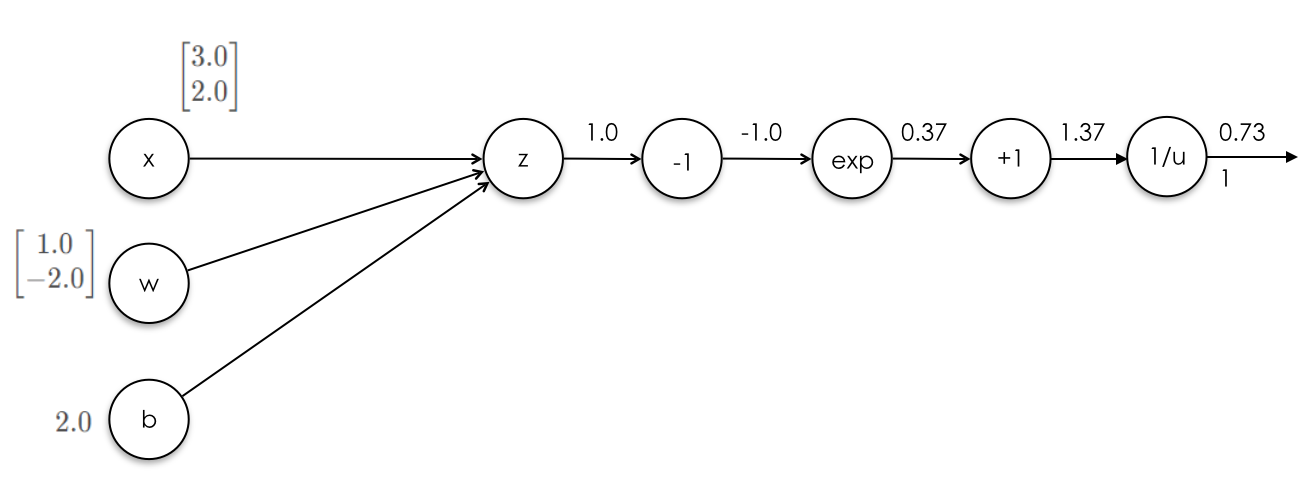
\includegraphics[height=5cm]{images/f000042}
\end{figure}
接下来我们来看反向传播的第一个节点1/u,该节点的微分为:
\begin{equation}
\begin{aligned}
u=1.37 \\
(1) \cdot \frac{d(\frac{1}{u})}{du}=-\frac{1}{u^2}=-\frac{1}{1.37^2}=-0.53
\end{aligned}
\label{mlp-sigmoid-cg-5}
\end{equation}
将微分值写在1/u节点左侧箭头线的下方,如下图所示:
\begin{figure}[H]
	\caption{计算图基本形式}
	\label{f000043}
	\centering
	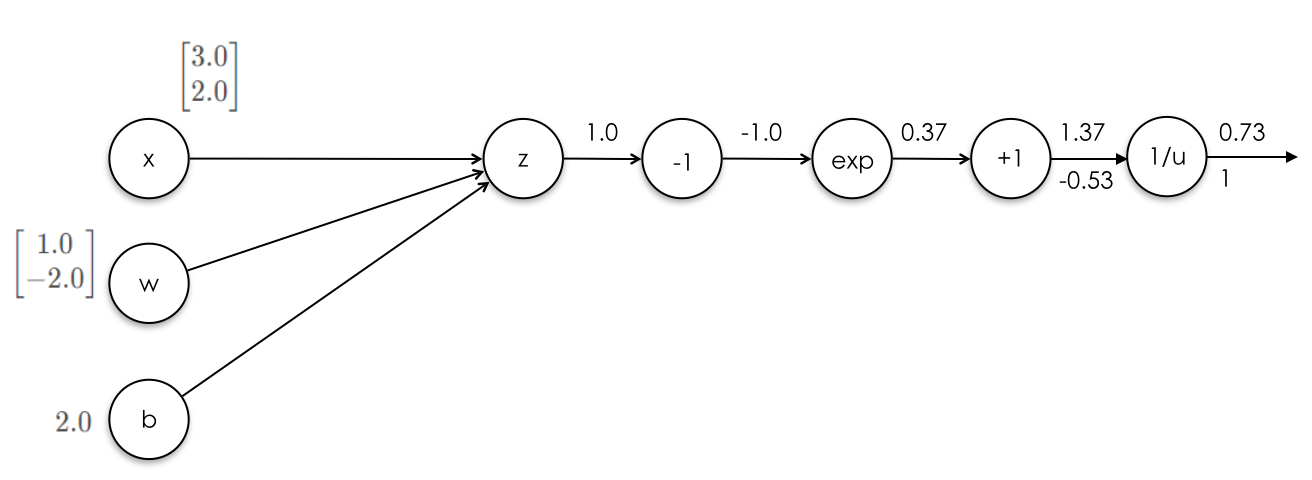
\includegraphics[height=5cm]{images/f000043}
\end{figure}
接着我们求u+1节点,计算公式如下所示:
\begin{equation}
\begin{aligned}
(-0.53) \cdot \frac{d(u+1)}{du}=(-0.53) \cdot 1=-0.53
\end{aligned}
\label{mlp-sigmoid-cg-6}
\end{equation}
将计算出的微分值写在+1节点左侧箭头线下方,如下所示:
\begin{figure}[H]
	\caption{计算图基本形式}
	\label{f000044}
	\centering
	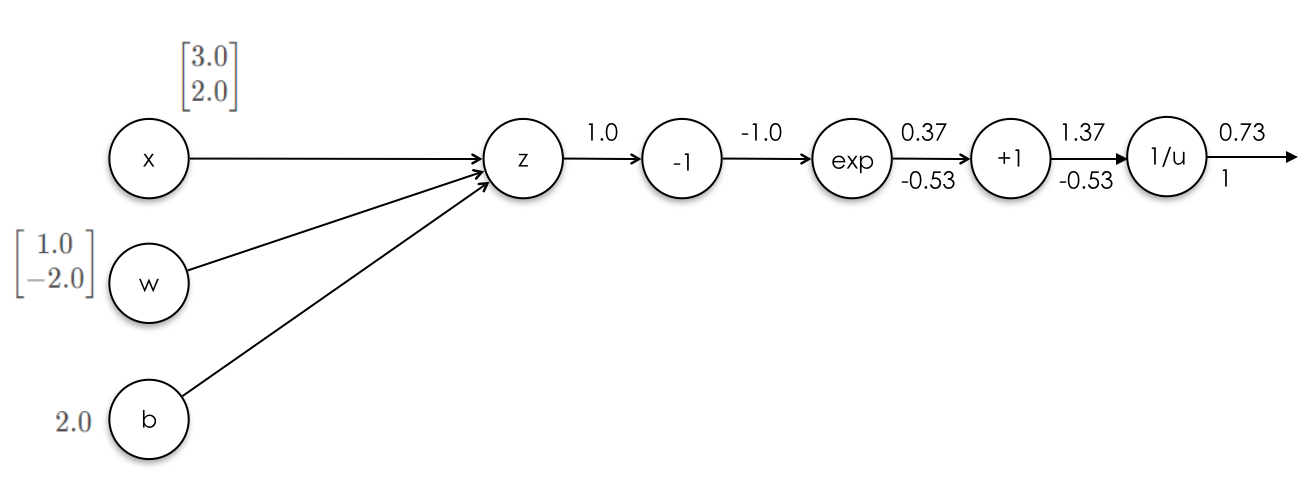
\includegraphics[height=5cm]{images/f000044}
\end{figure}

接下来我们处理exp节点,其微分计算公式为:
\begin{equation}
\begin{aligned}
(-0.53) \cdot \frac{de^u}{du}=(-0.53) \cdot e^u=(-0.53) \cdot 0.37=-0.20
\end{aligned}
\label{mlp-sigmoid-cg-7}
\end{equation}
式中$e^u$可以直接取正向传播时计算出的值,不必重新计算。将计算出的微分值写在exp节点左侧箭头线下方,如下图所示:
\begin{figure}[H]
	\caption{计算图基本形式}
	\label{f000045}
	\centering
	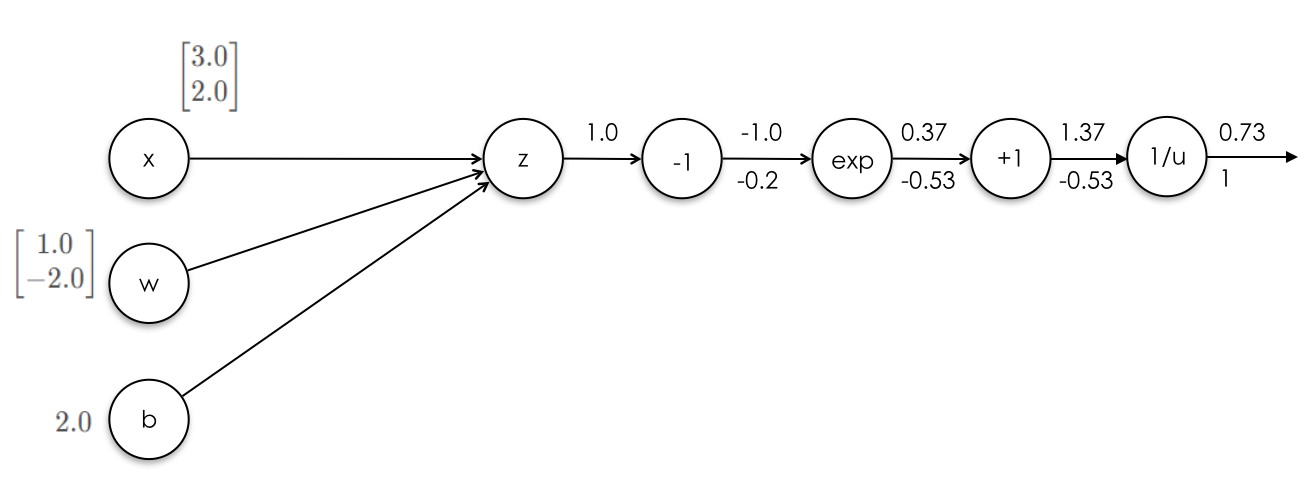
\includegraphics[height=5cm]{images/f000045}
\end{figure}
接下来我们处理取-1这个节点,微分计算公式为:
\begin{equation}
\begin{aligned}
(-0.20) \cdot \frac{d(-u)}{du}=(-0.20) \cdot (-1)=0.20
\end{aligned}
\label{mlp-sigmoid-cg-8}
\end{equation}
将微分值写在取-1节点左侧箭头线下方,如下图所示:
\begin{figure}[H]
	\caption{计算图基本形式}
	\label{f000046}
	\centering
	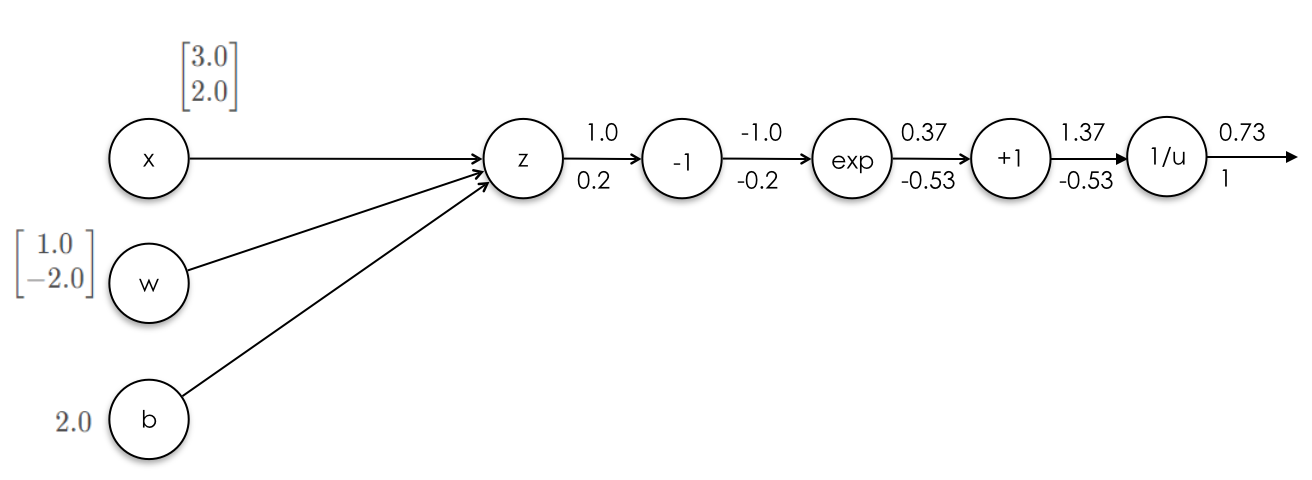
\includegraphics[height=5cm]{images/f000046}
\end{figure}
我们来处理z节点,为了演示概念,我们对$\boldsymbol{x}$也进行了求导,但是实际上我们只需要对网络参数进行求导。我们先对$\boldsymbol{x}$进行求导,微分计算公式为:
\begin{equation}
\begin{aligned}
(0.20) \cdot \frac{d(\boldsymbol{w}^T \cdot \boldsymbol{x}+b)}{d\boldsymbol{x}}=(0.20) \cdot \boldsymbol{w}=0.20 \cdot \begin{bmatrix}
1.0 \\
-2.0
\end{bmatrix}=\begin{bmatrix}
0.20 \\
-0.40
\end{bmatrix}
\end{aligned}
\label{mlp-sigmoid-cg-9}
\end{equation}
将求出的微分值写在$\boldsymbol{z}$与$\boldsymbol{x}$箭头线下方,如下图所示:
\begin{figure}[H]
	\caption{计算图基本形式}
	\label{f000047}
	\centering
	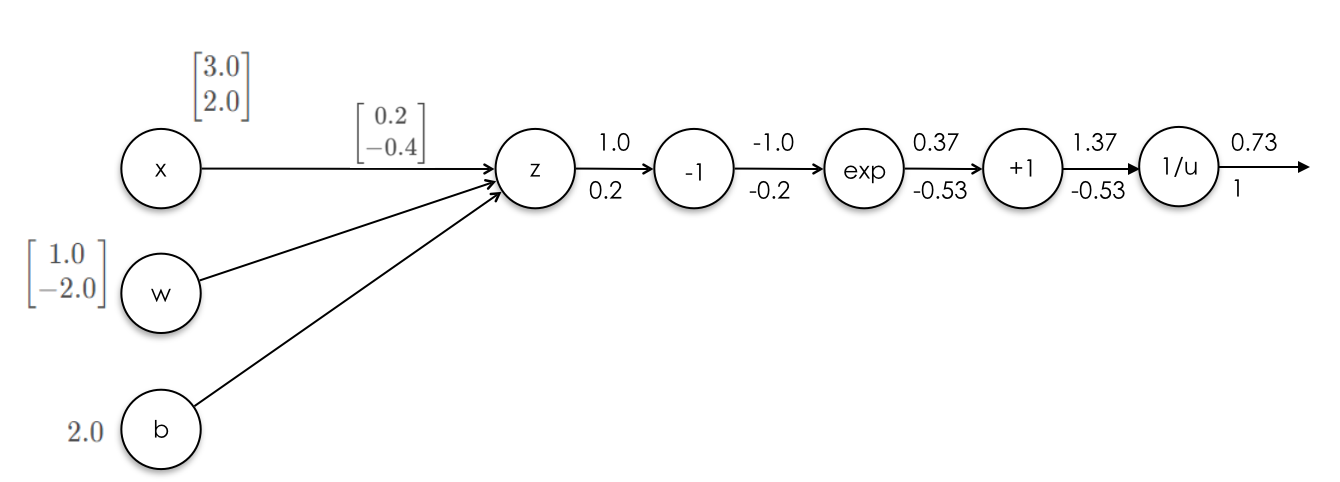
\includegraphics[height=5cm]{images/f000047}
\end{figure}
接下来我们对$\boldsymbol{z}$对$\boldsymbol{w}$的导数,微分计算公式为:
\begin{equation}
\begin{aligned}
(0.20) \cdot \frac{d(\boldsymbol{w}^T \cdot \boldsymbol{x}+b)}{d\boldsymbol{w}}=(0.20) \cdot \boldsymbol{x}=0.20 \cdot \begin{bmatrix}
3.0 \\
2.0
\end{bmatrix}=\begin{bmatrix}
0.60 \\
0.40
\end{bmatrix}
\end{aligned}
\label{mlp-sigmoid-cg-10}
\end{equation}

将计算出的微分值写在$\boldsymbol{z}$与$\boldsymbol{w}$之间箭头线的下方,如下图所示:
\begin{figure}[H]
	\caption{计算图基本形式}
	\label{f000048}
	\centering
	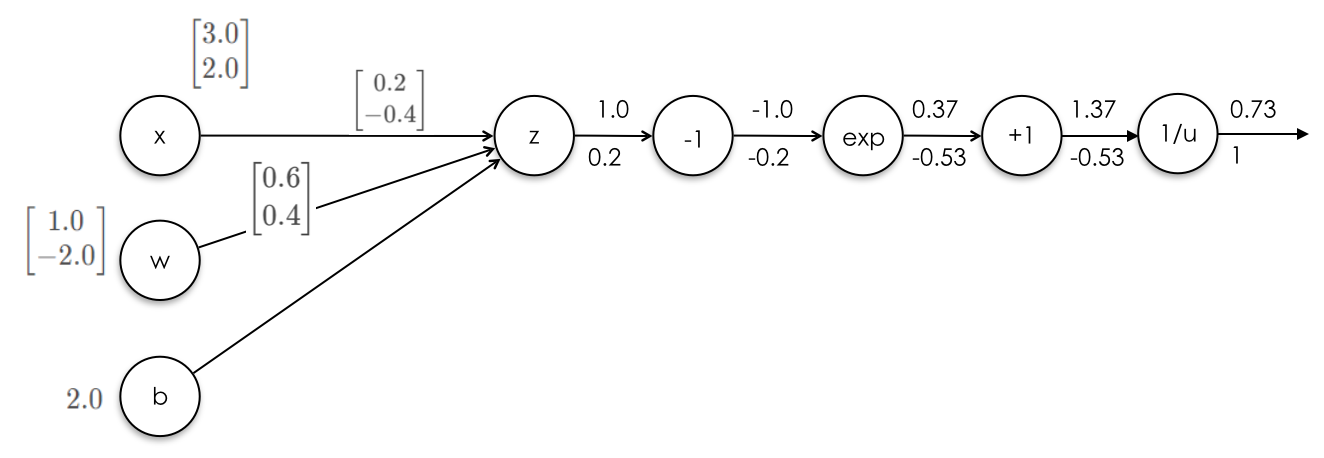
\includegraphics[height=5cm]{images/f000048}
\end{figure}
最后我们求$\boldsymbol{z}$对偏置值b的导数,计算公式如下所示:
\begin{equation}
\begin{aligned}
(0.20) \cdot \frac{d(\boldsymbol{w}^T \cdot \boldsymbol{x}+b)}{d\boldsymbol{b}}=(0.20) \cdot 1=0.20
\end{aligned}
\label{mlp-sigmoid-cg-11}
\end{equation}
将计算出的微分值写在$\boldsymbol{z}$与b之间箭头线的下方,如下图所示:
\begin{figure}[H]
	\caption{计算图基本形式}
	\label{f000049}
	\centering
	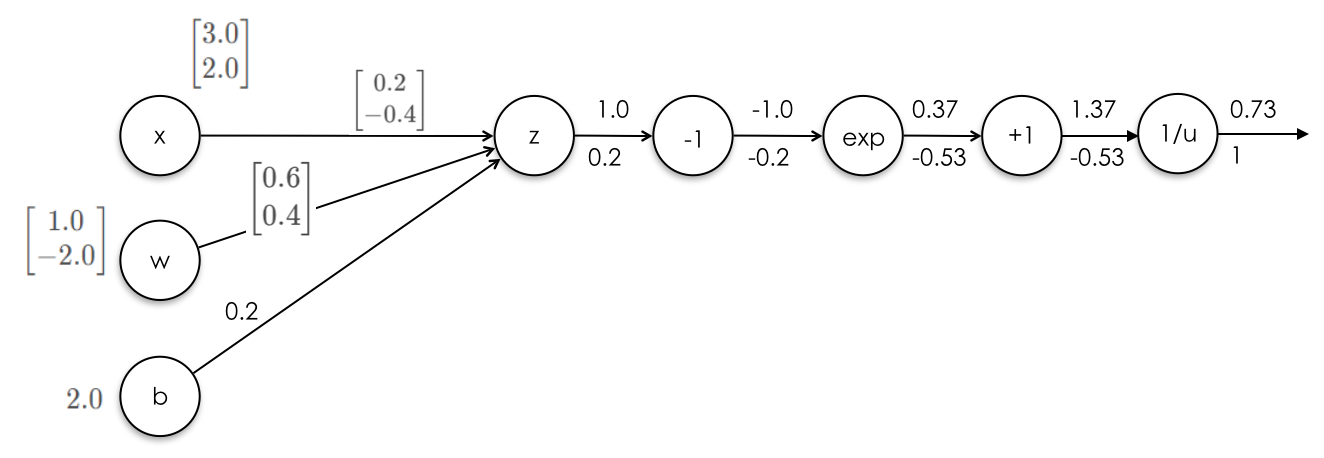
\includegraphics[height=5cm]{images/f000049}
\end{figure}
以上就是基于计算图的BP算法的计算过程,我们可以看出,无论多么复杂的函数,我们都能通过计算图求出该函数的导数。但是实际上我们还可以做的更好,因为基于计算图的模型中,我们为了反向传播,我们需要存储所有正向传播过程中的变量值,同时需要一步步反向运行正向过程。所以最近比较火的自动微分,就是重新建立一个用于微分的计算图,只需记录微分中用到的变量值,同时我们还可以根据函数求导的特点,设计简化的计算图。

\paragraph{自动微分}
如果关心深度学习的人,一定记得Yann LeCun说过:“深度学习已死,可微分编程永生”的话,就是说深度学习技术太受限了,可微分编程由于其灵活的特性,会成为未来具有巨大发展潜力的技术。而可微分编程的关键技术就是自动微分。自动微分就是重新构建一个计算微分的计算图,只需要将计算微分需要用到的变量值,保存到微分计算图中即可,然后就可以用与前向传播相同的方法来计算微分了。下面我们还以逻辑回归为例,来讲解自动微分技术。\newline
与计算图类似,我们首先完成信号的前向传播过程,接下来我们首先处理1/u节点,其计算公式为:
\begin{equation}
\begin{aligned}
\frac{d(\frac{1}{u})}{du}=-\frac{1}{u^2}
\end{aligned}
\label{mlp-sigmoid-cg-12}
\end{equation}
我们在正向计算图下面,画出我们微分计算图的第一个节点,如下图红色的节点:
\begin{figure}[H]
	\caption{自动微分}
	\label{f000050}
	\centering
	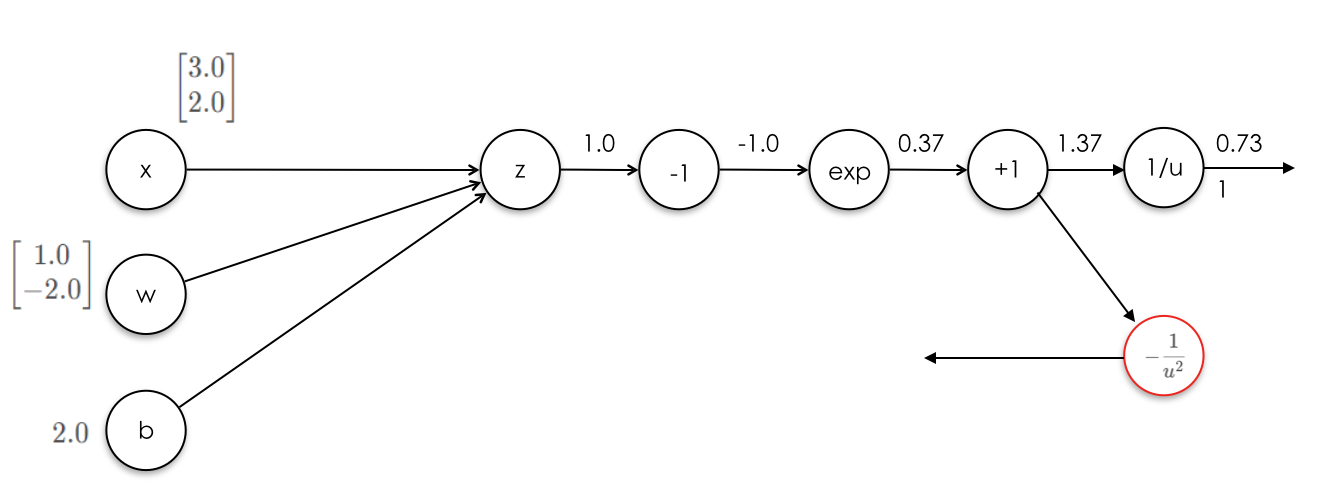
\includegraphics[height=5cm]{images/f000050}
\end{figure}
由于计算中需要u值,所以将正向传播时的u值保存到新节点中。\newline
接下来我们处理+1节点,计算公式如下所示:
\begin{equation}
\begin{aligned}
\frac{d(u+1)}{du}=1
\end{aligned}
\label{mlp-sigmoid-cg-13}
\end{equation}
所以我们需要在自动微分计算图中添加一个*1的节点,这时我们就不再需要保存前向传播的变量值了,这样就节省了空间,如下图所示:
\begin{figure}[H]
	\caption{自动微分}
	\label{f000051}
	\centering
	\includegraphics[height=5cm]{images/f000051}
\end{figure}
接下来我们来处理exp节点,计算公式如下所示:
\begin{equation}
\begin{aligned}
\frac{de^u}{du}=e^u
\end{aligned}
\label{mlp-sigmoid-cg-14}
\end{equation}

由于要计算中要用到$e^u$的值,所以需要在自动微分计算图中保存这个值,如下图所示:
\begin{figure}[H]
	\caption{自动微分}
	\label{f000052}
	\centering
	\includegraphics[height=5cm]{images/f000052}
\end{figure}
接下来我们处理取负节点,计算公式如下所示:
\begin{equation}
\begin{aligned}
\frac{d(-u)}{du}=-1
\end{aligned}
\label{mlp-sigmoid-cg-15}
\end{equation}
所以我们添加*(-1)节点,如下图所示:
\begin{figure}[H]
	\caption{自动微分}
	\label{f000053}
	\centering
	\includegraphics[height=5cm]{images/f000053}
\end{figure}
接下来我们处理z节点,我们这里先求z对x的微分,计算公式如下所示:
\begin{equation}
\begin{aligned}
\frac{d(\boldsymbol{w}^T \cdot \boldsymbol{x}+b)}{d\boldsymbol{w}}=\boldsymbol{x}
\end{aligned}
\label{mlp-sigmoid-cg-16}
\end{equation}
我们在自动微分计算图中添加如下节点:
\begin{figure}[H]
	\caption{自动微分}
	\label{f000054}
	\centering
	\includegraphics[height=5cm]{images/f000054}
\end{figure}
我们在这里就仅举$\boldsymbol{z}$对网络参数$\boldsymbol{w}$的微分为例。当有了计算图之后,我们求微分就和前向传播计算方式没有区别了。首先微分计算图的输入为1.37,运行第1个节点公式可得:
\begin{equation}
\begin{aligned}
-\frac{1}{u^2}=-\frac{1}{1.37^2}=-0.53
\end{aligned}
\label{mlp-sigmoid-cg-17}
\end{equation}
将计算结果写到图上,如下图所示:
\begin{figure}[H]
	\caption{自动微分}
	\label{f000055}
	\centering
	\includegraphics[height=5cm]{images/f000055}
\end{figure}
接下来我们处理*1节点,该节点只需简单的将前一步的微分值乘1即可,得到结果如下所示:
\begin{figure}[H]
	\caption{自动微分}
	\label{f000056}
	\centering
	\includegraphics[height=5cm]{images/f000056}
\end{figure}
接下来我们处理*这个节点,计算公式为:
\begin{equation}
\begin{aligned}
(-0.53)*e^u=(-0.53)*0.37=-0.20
\end{aligned}
\label{mlp-sigmoid-cg-18}
\end{equation}

处理结果如下所示:
\begin{figure}[H]
	\caption{自动微分}
	\label{f000057}
	\centering
	\includegraphics[height=5cm]{images/f000057}
\end{figure}
接下来处理*(-1)节点,只是在上一步微分结果上乘以-1即可,如下所示:
\begin{figure}[H]
	\caption{自动微分}
	\label{f000058}
	\centering
	\includegraphics[height=5cm]{images/f000058}
\end{figure}
接下来处理*节点,其是将上一步的微分值乘以$\boldsymbol{x}$,如下所示:
\begin{equation}
\begin{aligned}
(0.20) \cdot \boldsymbol{x}=(0.20) \cdot \begin{bmatrix}
3.0\\
2.0
\end{bmatrix}=\begin{bmatrix}
0.6\\
0.4
\end{bmatrix}
\end{aligned}
\label{mlp-sigmoid-cg-19}
\end{equation}
结果如下图所示:
\begin{figure}[H]
	\caption{自动微分}
	\label{f000059}
	\centering
	\includegraphics[height=5cm]{images/f000059}
\end{figure}
接着我们来看对偏置值b的导数,计算公式如下所示:
\begin{equation}
\begin{aligned}
\frac{d(\boldsymbol{w}^T \cdot \boldsymbol{x} + b)}{db}=1
\end{aligned}
\label{mlp-sigmoid-cg-20}
\end{equation}
所以最左边的节点就变成*1了,我们求出$\boldsymbol{z}$对b的微分,结果如下所示:
\begin{figure}[H]
	\caption{自动微分}
	\label{f000060}
	\centering
	\includegraphics[height=5cm]{images/f000060}
\end{figure}

\subsubsection{softmax和Cross Entropy}
我们在深度学习中遇到的最常见的问题就多分类问题,这时我们神经网络的输出层的激活函数softmax函数,代价函数取的是Cross Entropy函数。比较遗憾的是,关于这部数学原理的详细描述非常少,大部分都直接给出Cross Entropy用于softmax情形下的公式,直接拿来用就可以了。所以在这一节中,我们将详细介绍softmax函数和Cross Entropy函数应用于多分类问题的物理意义和数学推导过程。
\paragraph{多分类问题的表示}
我们在这里仍然以MNIST手写数字识别任务为例,我们要识别的类别为10类,分别为数字0$\sim$9,我们通常用one-hot向量形式来表示:
\begin{equation}
\begin{aligned}
\boldsymbol{y}=\begin{bmatrix}
y_1 & y_2 & y_3 & ... & y_k & ...& y_{10}
\end{bmatrix}=\begin{bmatrix}
0 & 0 & 0 & ... & 1 & ...& 0
\end{bmatrix}
\end{aligned}
\label{mlp-mnist-one-hot-vector}
\end{equation}

其中等于1的维所对应的数字就是我们希望的识别结果。\newline
通常我们神经网络的输出层为softmax函数,代表0$\sim$9这10个数字出现的概率,并且这些概率之和为1。
\begin{equation}
\begin{aligned}
\hat{\boldsymbol{y}}=\begin{bmatrix}
\hat{y}_1 & \hat{y}_2 & \hat{y}_3 & ... & \hat{y}_k & ...& \hat{y}_{10}
\end{bmatrix}
\end{aligned}
\label{mlp-mnist-y-hat-def}
\end{equation}
在数学上,我们可以把这个问题看成是有10个随机变量,分别对应0$\sim$9的出现事件,而对于某个数字对应的事件,其值只可能是出现和不出现两种,其符合我们数学上的Bernoulli分布,整个问题也就由这10个Bernoulli分布组成。我们首先来研究某个数字的Bernoulli分布。\newline
我们需要明确一点,我们现在研究的是识别任务的目标,也就是对应的$\boldsymbol{y}$,Bernoulli分布的定义如下所示:
\begin{equation}
\begin{aligned}
P(y=1)=\phi \\
P(y=0)=1-\phi \\
P(Y=y)=\phi^y \cdot (1-\phi)^{1-y}
\end{aligned}
\label{mlp-bernulli-def}
\end{equation}
式\ref{mlp-bernulli-def}中,$\phi$代表该事件出现的概率。
\paragraph{信息论简介}
信息论本来是研究在不可靠信道中,例如移动通信,怎样以最小的码长来可靠的传递信息的学科,理论体系非常庞大和复杂,对深度学习来讲,我们只需要知道在信息论中,如果知道最可能发生的事情发生了,那么我们得到的信息量非常小,而如果我们知道不可能发生的事件发生了,则我们得到的信息量将非常大。例如,如果我们知道今天太阳从东方升起,那么我们从中得不到任何有价值的信息,而如果我们知道今天早晨下了雪,路上湿滑,那么我们就知道应该注意出行安全,得到较多的有用信息。\newline
对于一个随机变量$\boldmath{x}$,取每个可能的值(在这里我们只计论离散值情况)就是一个事件$\boldmath{x}=x$,我们可以定义self information:
\begin{equation}
\begin{aligned}
I(x)=-\log\big( P(x) \big)
\end{aligned}
\label{mlp-self-information-def}
\end{equation}
在这里我们取的是以e为底的对数,单位是nats。\newline
如果我们把该随机变量所有出现的事件都集中起来,就得到信息论中的香农熵:
\begin{equation}
\begin{aligned}
H(\boldmath{x})=E_{\boldmath{x} \sim P}(I(\boldmath{x}))=-E_{\boldmath{x} \sim P}\big(\log{P(\boldmath{x})}\big)
\end{aligned}
\label{mlp-shannon-entropy-def}
\end{equation}
从式\ref{mlp-shannon-entropy-def}可以看出,香农熵可以定义为当$\boldmath{x}$符合P分布时,$\boldmath{x}$的self information的希望值。\newline
我们可以将在MNIST数据集上手写数字识别任务中,正确答案$\boldsymbol{y}$对某个数字的识别视为一个Bernoulli分布,将我们神经网络输出层softmax函数值输出中某个数字的识别,视为另一个Bernoulli分布,我们的目标就是让这两个分布尽可能接近。在信息论,对这个问题可以用KL散度来表示,我们假设正确答案所对应的分布为P,我们神经网络输出的分布为Q,则KL散度定义为:
\begin{equation}
\begin{aligned}
D_{KL}(P \Vert Q)=E_{\boldmath{x} \sim P}\begin{bmatrix}
\log{  \frac{P(x)}{Q(x)}  }
\end{bmatrix}=E_{\boldmath{x} \sim P}\begin{bmatrix}
\log{P(x)} - \log{Q(x)}
\end{bmatrix}
\end{aligned}
\label{mlp-kl-divergence-def}
\end{equation}
KL散度的值永远为正,而且当P和Q越接近其值越小,当P和Q是同一分布时,其值为零。但是KL散度有一个问题,就是$D_{KL}(P \Vert Q)$与$D_{KL}(Q \Vert P)$不相等,不完全等同于P和Q的距离。这就引出了我们的交叉熵Cross Entropy的定义:
\begin{equation}
\begin{aligned}
H(P,Q)=H(P) + D_{KL}(P \Vert Q)=-E_{\boldmath{x} \sim P}\begin{bmatrix}
\log{Q(x)}
\end{bmatrix}
\end{aligned}
\label{mlp-crossentropy-def}
\end{equation}
\paragraph{多分类问题的交叉熵表示}
回到我们MNIST手写数字识别任务,我们假设正确答案对某个数字识别的分布为P,神经网络输出对某个数字的概率的分布为Q,我们假设要研究的是第k维,即$y_k=1$,则有:
\begin{equation}
\begin{aligned}
CrossEntropy=H(P) + D_{KL}(P \Vert Q)=-E_{\boldmath{x} \sim P}\begin{bmatrix}
\log{Q(x)}
\end{bmatrix}=-\frac{1}{N_k}\sum_{i=1}^{N_k}\log{\hat{y}^{(i)}_k}
\end{aligned}
\label{mlp-mnist-crossentropy-def}
\end{equation}
其中$N_k$表示训练样本集中第k维等于1的样本数,我们对这些样本求出均值就是交叉熵函数了。为了便于处理,我们根据正确答案的特点,只有第k维是1,其余全为零,我们可以得到如下的计算公式:
\begin{equation}
\begin{aligned}
CrossEntropy=H(P) + D_{KL}(P \Vert Q)=-E_{\boldmath{x} \sim P}\begin{bmatrix}
\log{Q(x)}
\end{bmatrix}=-\frac{1}{N_k}\sum_{i=1}^{N_k}\log{\hat{y}^{(i)}_k}\\
=-\frac{1}{N_k}\sum_{i=1}^{N_k}\sum_{k=1}^{K=10}y_k \cdot \log{(\hat{y}^{(i)}_k)}
\end{aligned}
\label{mlp-mnist-crossentropy-formula}
\end{equation}
这个公式就是其他文档或教程里给出的Cross Entropy的公式,希望大家可以通过我们上面的推导过程,对交叉熵和softmax函数有更加深入的理解。\newline
以上我们讨论的是针对识别某个特定数字情况,而实际中有10个数字,处理方式完全相同,在训练样本集中包括所有这10个数字的识别样本,我们只需要将这些情况加在一起就可以了。
\paragraph{softmax求导}
softmax函数求导我们将以一种微稍不同的方式来讲解,大家在网络上或者教科书,对于softmax函数求导,都在在BP框架下进行的。但是当前流行的深度学习框架,如TensorFlow、Pytorch等,都是基于计算图模式,二者虽然原理相同,但是在具体处理方式上面,却有比较大的差异,在这一节中,我们将以PyTorch中采用的计算图的方式来进行讲解。\newline
对我们这个神经网络而言,我们采用Cross Entropy作为代价函数:
\begin{equation}
\begin{aligned}
L=-\sum_{i=1}^{K=10}y_i \cdot \log{(\hat{y}_i)}=-\log{(\hat{y}_k)}
\end{aligned}
\label{mlp-mnist-loss-function-crossentropy}
\end{equation}
我们在这里假设第k维为1,其余维均等于0。\newline
接下来我们定义代价函数对神经网络输出$\hat{\boldsymbol{y}}$求微分,这是一个标量对一个向量求微分,我们定义其结果为一个1行N列的矩阵,其中N为向量的维数,此时的代价函数只有第k维有值,其余维的值为0,所以可以表示为:
\begin{equation}
\begin{aligned}
\frac{\partial{L}}{\partial{\hat{\boldsymbol{y}}}}=\begin{bmatrix}
0 & 0 & ... & \big( -\log{\hat{y}_k} \big)' & ... & 0
\end{bmatrix}\\
=\begin{bmatrix}
0 & 0 & ... & -\frac{1}{\hat{y}_k} & ... & 0
\end{bmatrix}
\end{aligned}
\label{mlp-pL-pyhat}
\end{equation}
在这里我们用到了高等数学中的求导公式$(\log x)'=\frac{1}{x}$。
求出代价函数对输出层输出的微分之后,我们需要求输出层输出$\hat{\boldsymbol{y}}$对输出层输入$\boldsymbol{a}^2$的导数,这是一个向量对向量的导数,其中$\hat{\boldsymbol{y}} \in R^{N_2}$且$\boldsymbol{a}^2 \in R^{N_2}$,其中$N_2=10$。向量对向量的导数就是Jacobian矩阵,其定义为:
\begin{equation}
\begin{aligned}
\frac{\partial{\hat{\boldsymbol{y}}}}{\partial{\boldsymbol{a}^2}}=\begin{bmatrix}
\frac{\partial{\hat{y}_1}}{\partial{a^2_1}} & \frac{\partial{\hat{y}_1}}{\partial{a^2_2}} & ... & \frac{\partial{\hat{y}_1}}{\partial{a^2_{N_2}}} \\ \frac{\partial{\hat{y}_2}}{\partial{a^2_1}} & \frac{\partial{\hat{y}_2}}{\partial{a^2_2}} & ... & \frac{\partial{\hat{y}_2}}{\partial{a^2_{N_2}}} \\
... & ... & ... & ... \\
\frac{\partial{\hat{y}_{N_2}}}{\partial{a^2_1}} & \frac{\partial{\hat{y}_{N_2}}}{\partial{a^2_2}} & ... & \frac{\partial{\hat{y}_{N_2}}}{\partial{a^2_{N_2}}}
\end{bmatrix}
\end{aligned}
\label{mlp-pyhat-pa2}
\end{equation}
式\ref{mlp-pyhat-pa2}中$N_2=10$,所以式中的Jacobian矩阵是一个$R^{10 \times 10}$的方阵。\newline
下面我们来具体求解softmax函数的微分,由sfotmax函数定义可得:
\begin{equation}
\begin{aligned}
\hat{y}_i=\frac{e^{z_i}}{\sum_{j=1}^{K}e^{z_j}}
\end{aligned}
\label{mlp-softmax-def-for-i-element}
\end{equation}

对于$\frac{\partial{\hat{y}_i}}{\partial{z_j}}$,我们分两种情况来讨论。\newline
当$i=j$时:
\begin{equation}
\begin{aligned}
\frac{\partial{\hat{y}_i}}{\partial{z_i}}=\frac{\big( e^{z_i} \big)' \cdot \sum_{j=1}^{K}e^{z_j} - e^{z_i} \cdot \big( \sum_{j=1}^{K}e^{z_j} \big)'}{\big( \sum_{j=1}^{K}e^{z_j} \big)^2}\\
=\frac{e^{z_i} \cdot \sum_{j=1}^{K}e^{z_j} - e^{z_i} \cdot e^{z_i}}{\big( \sum_{j=1}^{K}e^{z_j} \big)^2}\\
=\frac{e^{z_i}}{\sum_{j=1}^{K}e^{z_j}} \cdot \frac{\sum_{j=1}^{K}e^{z_j} - e^{z_i}}{\sum_{j=1}^{K}e^{z_j}}\\
=\frac{e^{z_i}}{\sum_{j=1}^{K}e^{z_j}} \cdot \bigg( 1-\frac{e^{z_i}}{\sum_{j=1}^{K}e^{z_j}} \bigg)\\
=\hat{y}_i \cdot \big( 1 - \hat{y}_i \big)
\end{aligned}
\label{mlp-softmax-devirative-i=j}
\end{equation}
当$i \ne j$时:
\begin{equation}
\begin{aligned}
\frac{\partial{\hat{y}_i}}{\partial{z_j}}=e^{z_i} \cdot \bigg( -\frac{(\sum_{j=1}^{K}e^{z_j})'}{(\sum_{j=1}^{K}e^{z_j})^2} \bigg)\\
=-\frac{e^{z_i} \cdot e^{z_j}}{(\sum_{j=1}^{K}e^{z_j})^2}\\
=-\frac{e^{z_i}}{\sum_{j=1}^{K}e^{z_j}} \cdot \frac{e^{z_j}}{\sum_{j=1}^{K}e^{z_j}}\\
=-\hat{y}_i \cdot \hat{y}_j
\end{aligned}
\label{mlp-softmax-devirative-i!=j}
\end{equation}
综上所述,对Jacobian矩阵$\frac{\partial{\hat{\boldsymbol{y}}}}{\partial{\boldsymbol{z}^2}}$,对角线上元素可以用式\ref{mlp-softmax-devirative-i=j}来表示,而非对角线上元素可以用式\ref{mlp-softmax-devirative-i!=j}来表示。

\subsubsection{计算图简介}
我们所研究网络的计算图如下所示:
\begin{figure}[H]
	\caption{神经网络计算图表示}
	\label{f000061}
	\centering
	\includegraphics[height=5cm]{images/f000061}
\end{figure}
计算图分为两个阶段:信号前向传播和误差反向传播。\newline
\paragraph{正向传播}
我们先来看信号前向传播过程,输入信号为原始图像$\boldsymbol{x}$,可以得到第1层的输入:
\begin{equation}
\begin{aligned}
\boldsymbol{z}^1=W^1 \cdot \boldsymbol{x} + \boldsymbol{b}^1
\end{aligned}
\label{mlp-cg-forward-1}
\end{equation}
求出第1层神经元输入后,应用神经元激活函数,得到第1层的输出:
\begin{equation}
\begin{aligned}
\boldsymbol{a}^1=f(\boldsymbol{z}^1)
\end{aligned}
\label{mlp-cg-forward-2}
\end{equation}
接着我们求出第2层的输入信号:
\begin{equation}
\begin{aligned}
\boldsymbol{z}^2=W^2 \cdot \boldsymbol{a}^1 + \boldsymbol{b}^2
\end{aligned}
\label{mlp-cg-forward-3}
\end{equation}
接着求出第2层的输出,由于第2层即为输出层,所以也就是求出$\hat{\boldsymbol{y}}$:
\begin{equation}
\begin{aligned}
\hat{y}_i=\frac{e^{z_i}}{\sum_{j=1}^{K}e^{z_j}}
\end{aligned}
\label{mlp-cg-forward-4}
\end{equation}

我们取出正确结果$\boldsymbol{y}$,采用Cross Entropy作为代价函数,这里我们假设第k维等于1,其他维均为零:
\begin{equation}
\begin{aligned}
C=-\sum_{i=1}^{K}y_i \cdot \log{(\hat{y}_i)}=-\log(\hat{y}_k)
\end{aligned}
\label{mlp-cg-forward-5}
\end{equation}
\paragraph{反向传播}
反向传播阶段就是求出图\ref{f000026}中在连接上的微分值。对我们这个神经网络而言,我们采用Cross Entropy作为代价函数:
\begin{equation}
\begin{aligned}
L=-\sum_{i=1}^{K=10}y_i \cdot \log{(\hat{y}_i)}=-\log{(\hat{y}_k)}
\end{aligned}
\label{mlp-cg-backward-1}
\end{equation}
我们在这里假设第k维为1,其余维均等于0。\newline
接下来我们定义代价函数对神经网络输出$\hat{\boldsymbol{y}}$求微分,这是一个标量对一个向量求微分,我们定义其结果为一个1行N列的矩阵,其中N为向量的维数,此时的代价函数只有第k维有值,其余维的值为0,所以可以表示为:
\begin{equation}
\begin{aligned}
\frac{\partial{L}}{\partial{\hat{\boldsymbol{y}}}}=\begin{bmatrix}
0 & 0 & ... & \big( -\log{\hat{y}_k} \big)' & ... & 0
\end{bmatrix}\\
=\begin{bmatrix}
0 & 0 & ... & -\frac{1}{\hat{y}_k} & ... & 0
\end{bmatrix}
\end{aligned}
\label{mlp-cg-backward-2}
\end{equation}
在这里我们用到了高等数学中的求导公式$(\log x)'=\frac{1}{x}$。
求出代价函数对输出层输出的微分之后,我们需要求输出层输出$\hat{\boldsymbol{y}}$对输出层输入$\boldsymbol{z}^2$的导数,这是一个向量对向量的导数,其中$\hat{\boldsymbol{y}} \in R^{N_2}$且$\boldsymbol{z}^2 \in R^{N_2}$,其中$N_2=10$。向量对向量的导数就是Jacobian矩阵,其定义为:
\begin{equation}
\begin{aligned}
\frac{\partial{\hat{\boldsymbol{y}}}}{\partial{\boldsymbol{z}^2}}=\begin{bmatrix}
\frac{\partial{\hat{y}_1}}{\partial{z^2_1}} & \frac{\partial{\hat{y}_1}}{\partial{z^2_2}} & ... & \frac{\partial{\hat{y}_1}}{\partial{z^2_{N_2}}} \\ \frac{\partial{\hat{y}_2}}{\partial{z^2_1}} & \frac{\partial{\hat{y}_2}}{\partial{z^2_2}} & ... & \frac{\partial{\hat{y}_2}}{\partial{z^2_{N_2}}} \\
... & ... & ... & ... \\
\frac{\partial{\hat{y}_{N_2}}}{\partial{z^2_1}} & \frac{\partial{\hat{y}_{N_2}}}{\partial{z^2_2}} & ... & \frac{\partial{\hat{y}_{N_2}}}{\partial{z^2_{N_2}}}
\end{bmatrix}=\begin{bmatrix}
\hat{y}_1 \cdot (1-\hat{y}_1) & -\hat{y}_1 \cdot \hat{y}_2 & ... & -\hat{y}_1 \cdot \hat{y}_{N_2} \\
-\hat{y}_2 \cdot \hat{y}_1 & \hat{y}_2 \cdot (1-\hat{y}_2) & ... & -\hat{y}_1 \cdot \hat{y}_{N_2} \\
-\hat{y}_{N_2} \cdot \hat{y}_1 & -\hat{y}_{N_2} \cdot \hat{y}_2 & ... & \hat{y}_{N_2} \cdot (1-\hat{y}_{N_2})
\end{bmatrix}
\end{aligned}
\label{mlp-cg-backward-3}
\end{equation}
式\ref{mlp-cg-backward-3}中$N_2=10$,所以式中的Jacobzian矩阵是一个$R^{10 \times 10}$的方阵。\newline
下面我们来具体求解softmax函数的微分,由sfotmax函数定义可得:
\begin{equation}
\begin{aligned}
\hat{y}_i=\frac{e^{z_i}}{\sum_{j=1}^{K}e^{z_j}}
\end{aligned}
\label{mlp-cg-backward-4}
\end{equation}
对于$\frac{\partial{\hat{y}_i}}{\partial{z_j}}$,我们分两种情况来讨论。\newline
当$i=j$时:
\begin{equation}
\begin{aligned}
\frac{\partial{\hat{y}_i}}{\partial{z_i}}=\frac{\big( e^{z_i} \big)' \cdot \sum_{j=1}^{K}e^{z_j} - e^{z_i} \cdot \big( \sum_{j=1}^{K}e^{z_j} \big)'}{\big( \sum_{j=1}^{K}e^{z_j} \big)^2}\\
=\frac{e^{z_i} \cdot \sum_{j=1}^{K}e^{z_j} - e^{z_i} \cdot e^{z_i}}{\big( \sum_{j=1}^{K}e^{z_j} \big)^2}\\
=\frac{e^{z_i}}{\sum_{j=1}^{K}e^{z_j}} \cdot \frac{\sum_{j=1}^{K}e^{z_j} - e^{z_i}}{\sum_{j=1}^{K}e^{z_j}}\\
=\frac{e^{z_i}}{\sum_{j=1}^{K}e^{z_j}} \cdot \bigg( 1-\frac{e^{z_i}}{\sum_{j=1}^{K}e^{z_j}} \bigg)\\
=\hat{y}_i \cdot \big( 1 - \hat{y}_i \big)
\end{aligned}
\label{mlp-cg-backward-5}
\end{equation}
当$i \ne j$时:
\begin{equation}
\begin{aligned}
\frac{\partial{\hat{y}_i}}{\partial{z_j}}=e^{z_i} \cdot \bigg( -\frac{(\sum_{j=1}^{K}e^{z_j})'}{(\sum_{j=1}^{K}e^{z_j})^2} \bigg)\\
=-\frac{e^{z_i} \cdot e^{z_j}}{(\sum_{j=1}^{K}e^{z_j})^2}\\
=-\frac{e^{z_i}}{\sum_{j=1}^{K}e^{z_j}} \cdot \frac{e^{z_j}}{\sum_{j=1}^{K}e^{z_j}}\\
=-\hat{y}_i \cdot \hat{y}_j
\end{aligned}
\label{mlp-cg-backward-6}
\end{equation}
综上所述,对Jacobian矩阵$\frac{\partial{\hat{\boldsymbol{y}}}}{\partial{\boldsymbol{a}^2}}$,对角线上元素可以用式\ref{mlp-cg-backward-5}来表示,而非对角线上元素可以用式\ref{mlp-cg-backward-6}来表示。\newline
接下来我们求$\frac{\partial{\boldsymbol{z}^2}}{\partial{\boldsymbol{a}^1}}$的值,我们首先计算单个值的微分:
\begin{equation}
\begin{aligned}
\frac{\partial{z^2_i}}{\partial{a^1_j}}=\frac{\partial{(W^2_{i,1}\cdot a^1_1 + W^2_{i,2}\cdot a^1_2 + ... + W^2_{i,j}\cdot a^1_{j} + ... + W^2_{i,N_1}\cdot a^1_{N_1} + b^2_1)}} {\partial{a^1_j}}=W^2_{i,j}
\end{aligned}
\label{mlp-cg-backward-7}
\end{equation}
由式\ref{mlp-cg-backward-7}可得:
\begin{equation}
\begin{aligned}
\frac{\partial{\boldsymbol{z}^2}}{\partial{\boldsymbol{a}^1}}=\begin{bmatrix}
W^2_{1,1} & W^2_{1,2} & ... & W^2_{1,N_1} \\
W^2_{2,1} & W^2_{2,2} & ... & W^2_{2,N_1} \\
... & ... & ... & ... \\

W^2_{N_2,1} & W^2_{N_2,2} & ... & W^2_{N_2,N_1}
\end{bmatrix}=W^2
\end{aligned}
\label{mlp-cg-backward-8}
\end{equation}
在接下来我们求$\frac{\partial{\boldsymbol{z}^2}}{\partial{W^2}}$的值,这时我们求的是向量对矩阵的微分,我们可以将$W^2$视为一个行向量组成的向量,如下所示:
\begin{equation}
\begin{aligned}
W^2=\begin{bmatrix}
W^2_{1,1} & W^2_{1,2} & ... & W^2_{1,N_1} \\
W^2_{2,1} & W^2_{2,2} & ... & W^2_{2,N_1} \\
... & ... & ... & ... \\

W^2_{N_2,1} & W^2_{N_2,2} & ... & W^2_{N_2,N_1}
\end{bmatrix}=\begin{bmatrix}
\boldsymbol{w}_1 \\
\boldsymbol{w}_2 \\
... \\
\boldsymbol{w}_{N_2} \\
\end{bmatrix}
\end{aligned}
\label{mlp-cg-backward-9}
\end{equation}
这样我们就把问题变为向量对向量求微分形式了,根据Jacobian矩阵定义可得:
\begin{equation}
\begin{aligned}
\frac{\partial{\boldsymbol{z}^2}}{\partial{W^2}}=\begin{bmatrix}
\frac{\partial{z^2_1}}{\partial{\boldsymbol{w}_1}} & \frac{\partial{z^2_1}}{\partial{\boldsymbol{w}_2}} & ... & \frac{\partial{z^2_1}}{\partial{\boldsymbol{w}_{N_2}}} \\
\frac{\partial{z^2_2}}{\partial{\boldsymbol{w}_1}} & \frac{\partial{z^2_2}}{\partial{\boldsymbol{w}_2}} & ... & \frac{\partial{z^2_2}}{\partial{\boldsymbol{w}_{N_2}}} \\
... & ... & ... & ... \\

\frac{\partial{z^2_{N_2}}}{\partial{\boldsymbol{w}_1}} & \frac{\partial{z^2_{}}}{\partial{\boldsymbol{w}_2}} & ... & \frac{\partial{z^2_{N_2}}}{\partial{\boldsymbol{w}_{N_2}}}
\end{bmatrix}
\end{aligned}
\label{mlp-cg-backward-10}
\end{equation}
在式\ref{mlp-cg-backward-10}的矩阵中的每一项均是一个标量对向量的求导,结果为一个只有一行的矩阵,维度为向量的维度,所以其维度为$N_1$。我们来看任意一项的微分$\frac{\partial{z^2_i}} {\partial{W^2_{j,k}}}$。
当$i \ne j$时:此时连接权值$W^2_{j,k}$不指向第2层第i个节点,此时求微分值为零,由此可知,式\ref{e000037}中,非对角线上的元素,其值为元素值全为0的向量,维度为$N_1$。
当$i=j$时:
由第2层神经元输入信号计算公式:
\begin{equation}
\begin{aligned}
z^2_i=W^2_{i,1} \cdot a^1_1 + W^2_{i,2} \cdot a^1_2 + ... + W^2_{i,N_1} \cdot a^1_{N_1} + b^2_i
\end{aligned}
\label{mlp-cg-backward-11}
\end{equation}
可得:
\begin{equation}
\begin{aligned}
\frac{\partial{z^2_i}}{\partial{W^2_{i,k}}}=\frac{\partial{(W^2_{i,1} \cdot a^1_1 + W^2_{i,2} \cdot a^1_2 + ... + W^2_{i,N_1} \cdot a^1_{N_1} + b^2_i)}} {\partial{W^2_{i,k}}}=a^1_k
\end{aligned}
\label{mlp-cg-backward-12}
\end{equation}
由式\ref{mlp-cg-backward-12}可知,式\ref{mlp-cg-backward-10}中不为零的对角线上元素为$R^{1 \times {N_1}}$只有一行的矩阵,其值为第1层神经元的输出。如下所示:
\begin{equation}
\begin{aligned}
\frac{\partial{\boldsymbol{z}^2}}{\partial{W^2}}=\begin{bmatrix}
\frac{\partial{z^2_1}}{\partial{\boldsymbol{w}_1}} & \frac{\partial{z^2_1}}{\partial{\boldsymbol{w}_2}} & ... & \frac{\partial{z^2_1}}{\partial{\boldsymbol{w}_{N_2}}} \\
\frac{\partial{z^2_2}}{\partial{\boldsymbol{w}_1}} & \frac{\partial{z^2_2}}{\partial{\boldsymbol{w}_2}} & ... & \frac{\partial{z^2_2}}{\partial{\boldsymbol{w}_{N_2}}} \\
... & ... & ... & ... \\
\frac{\partial{z^2_{N_2}}}{\partial{\boldsymbol{w}_1}} & \frac{\partial{z^2_{N_2}}}{\partial{\boldsymbol{w}_2}} & ... & \frac{\partial{z^2_{N_2}}}{\partial{\boldsymbol{w}_{N_2}}}
\end{bmatrix}=\begin{bmatrix}
\boldsymbol{a}^1 & \boldsymbol{0} & ... & \boldsymbol{0} \\
\boldsymbol{0} & \boldsymbol{a}^1 & ... & \boldsymbol{0} \\
\boldsymbol{0} & \boldsymbol{0} & ... & \boldsymbol{a}^1
\end{bmatrix}
\end{aligned}
\label{mlp-cg-backward-13}
\end{equation}
接下来我们求$\frac{\partial{\boldsymbol{z}^2}}{\partial{\boldsymbol{b}^2}}$,由Jacobian矩阵定义可得:
\begin{equation}
\begin{aligned}
\frac{\partial{\boldsymbol{z}^2}}{\partial{\boldsymbol{b}^2}}=\begin{bmatrix}
\frac{\partial{z^2_1}}{\partial{b^2_1}} & \frac{\partial{z^2_1}}{\partial{b^2_1}} & ... & \frac{\partial{z^2_1}}{\partial{b^2_{N_2}}}\\
\frac{\partial{z^2_1}}{\partial{b^2_1}} & \frac{\partial{z^2_1}}{\partial{b^2_1}} & ... & \frac{\partial{z^2_1}}{\partial{b^2_{N_2}}}\\
... & ... & ... & ... \\
\frac{\partial{z^2_{N_2}}}{\partial{b^2_1}} & \frac{\partial{z^2_{N_2}}}{\partial{b^2_1}} & ... & \frac{\partial{z^2_{N_2}}}{\partial{b^2_{N_2}}}\\
\end{bmatrix}=\begin{bmatrix}
1 & 0 & ... & 0 \\
0 & 1 & ... & 0 \\
0 & 0 & ... & 1
\end{bmatrix}
\end{aligned}
\label{mlp-cg-backward-14}
\end{equation}
对于矩阵中任意元素$\frac{\partial{z^2_i}}{\partial{b^2_j}}$,其公式为:
\begin{equation}
\begin{aligned}
\frac{\partial{z^2_i}}{\partial{b^2_j}}=\frac{\partial{(W^2_{i,1} \cdot a^1_1 + W^2_{i,2} \cdot a^1_2 + ... + W^2_{i,N_1} \cdot a^1_{N_1} + b^2_i)}}{\partial{b^2_j}}
\end{aligned}
\label{mlp-cg-backward-15}
\end{equation}
当$i \ne j$时,式\ref{mlp-cg-backward-15}的值为0,当$i=j$时,其值为1,所以最终结果为$R^{N_2 \times N_2}$的单位阵。
采用同样方式,我们可以求出$\frac{\partial{\boldsymbol{z}^1}}{\partial{W^1}}$和$\frac{\partial{\boldsymbol{z}^1}}{\partial{\boldsymbol{b}^1}}$的微分,从而完成反向传播过程。注意:在反向传播过程中,我们只求与网络参数有关的微分,我们一般不求对$\boldsymbol{x}$的微分。
\paragraph{网络参数求微分}
计算完所有微分值后,我们就可求网络参数对于代价函数的偏微分了。
\begin{equation}
\begin{aligned}
\frac{\partial{C}}{\partial{W^2}}=\frac{\partial{C}}{\partial{\hat{\boldsymbol{y}}}} \cdot \frac{\partial{\hat{\boldsymbol{y}}}}{\partial{\boldsymbol{z^2}}} \cdot \frac{\partial{\boldsymbol{z^2}}}{\partial{W^2}}
\end{aligned}
\label{mlp-cg-backward-16}
\end{equation}

\begin{equation}
\begin{aligned}
\frac{\partial{C}}{\partial{\boldsymbol{b}^2}}=\frac{\partial{C}}{\partial{\hat{\boldsymbol{y}}}} \cdot \frac{\partial{\hat{\boldsymbol{y}}}}{\partial{\boldsymbol{z^2}}} \cdot \frac{\partial{\boldsymbol{z^2}}}{\partial{\boldsymbol{b}^2}}
\end{aligned}
\label{mlp-cg-backward-17}
\end{equation}

\begin{equation}
\begin{aligned}
\frac{\partial{C}}{\partial{\boldsymbol{b}^1}}=\frac{\partial{C}}{\partial{\hat{\boldsymbol{y}}}} \cdot \frac{\partial{\hat{\boldsymbol{y}}}}{\partial{\boldsymbol{z^2}}} \cdot \frac{\partial{\boldsymbol{z^2}}}{\partial{\boldsymbol{a}^1}} \cdot \frac{\partial{\boldsymbol{a^1}}}{\partial{\boldsymbol{z}^1}} \cdot \frac{\partial{\boldsymbol{z^1}}}{\partial{\boldsymbol{b}^1}}
\end{aligned}
\label{mlp-cg-backward-18}
\end{equation}

\begin{equation}
\begin{aligned}
\frac{\partial{C}}{\partial{W^1}}=\frac{\partial{C}}{\partial{\hat{\boldsymbol{y}}}} \cdot \frac{\partial{\hat{\boldsymbol{y}}}}{\partial{\boldsymbol{z^2}}} \cdot \frac{\partial{\boldsymbol{z^2}}}{\partial{\boldsymbol{a}^1}} \cdot \frac{\partial{\boldsymbol{a^1}}}{\partial{\boldsymbol{z}^1}} \cdot \frac{\partial{\boldsymbol{z^1}}}{\partial{W^1}}
\end{aligned}
\label{mlp-cg-backward-19}
\end{equation}

\paragraph{梯度下降算法调参数}
当求出网络参数的微分之后,就可以使用各种优化算法来调整网络的参数了,例如采用梯度下降算法,我们假设学习率为$\alpha > 0$:
\begin{equation}
\begin{aligned}
W^2=W^2 - \alpha \cdot \frac{\partial{C}}{\partial{W^2}}
\end{aligned}
\label{mlp-cg-backward-20}
\end{equation}

\begin{equation}
\begin{aligned}
\boldsymbol{b}^2=\boldsymbol{b}^2 - \alpha \cdot \frac{\partial{C}}{\partial{\boldsymbol{b}^2}}
\end{aligned}
\label{mlp-cg-backward-21}
\end{equation}

\begin{equation}
\begin{aligned}
W^1=W^1 - \alpha \cdot \frac{\partial{C}}{\partial{W^1}}
\end{aligned}
\label{mlp-cg-backward-22}
\end{equation}

\begin{equation}
\begin{aligned}
\boldsymbol{b}^1=\boldsymbol{b}^1 - \alpha \cdot \frac{\partial{C}}{\partial{\boldsymbol{b}^1}}
\end{aligned}
\label{mlp-cg-backward-23}
\end{equation}
在这里我们只讨论了一个简化再简化的版本,忽略很多细节,例如我们并没有考虑迷你批次问题,而使用的是在线学习的算法,即每次只学习一个样本,而实际工程中,我们会拿例如128个样本一次性进行学习,还有就为了增加网络的泛化能力,我们一般会增加$L_2$调整项,就是代价函数在Cross Entropy函数基础上,再加上一个调整项:
\begin{equation}
\begin{aligned}
\boldmath{L}=C+\omega=C+ \lambda \cdot \sum_{l=1}^{L} \Vert W^l \Vert _2
\end{aligned}
\label{mlp-cg-backward-24}
\end{equation}

\subsubsection{Softmax层实现技术}
在前两节中,我们详细讲解反向传播的链式求导和计算图法,这也是TensorFlow、Pytorch的底层实现技术。但是如果我们利用Numpy手工实现的话,由于我们的网络结构完全确定,完全复现这些计算过程,显然会非常浪费计算资源,在实际中我们会只利用最后的计算结果,而忽略其中的计算过程。
\paragraph{在线学习}
我们在实际应用中,网络的输出层通常采用Softmax激活函数,而代价函数通常采用CrossEntropy,因此通常的处理方法为将输出层和代价函数层合而为一,一次性计算出网络输出$\hat{\boldsymbol{y}}^{(i)}$、代价函数值$\mathcal{J}$、代价函数对连接权值的微分$\frac{\partial{\mathcal{J}}}{\partial{W}}$、代价函数对本层偏置值的微分$\frac{\partial{\mathcal{J}}}{\partial{\boldsymbol{b}}}$、代价函数对上一层输出的微分$\frac{\partial{\mathcal{J}}}{\partial{\boldsymbol{x}}}$。下面我们分别来看这些值的求法。\newline
在线学习就是一次学习一个样本,在下面的公式推导中,如本层的输入线性和$\boldsymbol{z}^{l,(i)}$代表第$l$层第$i$个样本的线性输入信号,在下面为了公式推层的简洁性,我们将省略上标。同时我们将上一层的输出定义为$\boldsymbol{x} \in R^n$。我们假设共有$m$个样本,样本特征数为$n$,共有$K$个类别。\newline
我们的代价函数采用交叉熵(CrossEntropy)形式,可以表求为如下形式:
\begin{equation}
\mathcal{J}=-\boldsymbol{y} \log{\hat{\boldsymbol{y}}} \rightarrow np.sum(\begin{bmatrix}
0 \\
0 \\
... \\
-\log{\hat{y}_{r}} \\
... \\
0
\end{bmatrix})=-\log{\hat{y}_{r}}
\label{mlp-cross-entropy-vector-def}
\end{equation}
式中的相乘是elementwise相乘,最后通过numpy.sum进行求和,得到一个标量值。其中$r$为是第$r$类。\newline
接下来我们将代价函数对$\hat{\boldsymbol{y}}$求微分,根据向量微分章节中标量对向量微分可得:
\begin{equation}
\frac{\partial{\mathcal{J}}}{\partial{\hat{\boldsymbol{y}}}} = \begin{bmatrix}
0 & 0 & ... & -\frac{1}{\hat{y}_{r}} & ... & 0
\end{bmatrix} \in R^{1 \times K}
\label{mlp-pj-py-def}
\end{equation}
接下来我们求本层输出对本层线性输入的微分,根据我们在前面推导的softmax函数微分公式:
\begin{equation}
\frac{\partial{\hat{\boldsymbol{y}}}}{\partial{\boldsymbol{z}}}=\begin{bmatrix}
\hat{y}_{1}(1-\hat{y_{1}}) & -\hat{y_{1}}\hat{y_{2}} & ... & -\hat{y_{1}}\hat{y_{K}} \\
-\hat{y_{2}}\hat{y_{1}} & \hat{y}_{2}(1-\hat{y_{2}}) & ... & -\hat{y_{2}}\hat{y_{K}} \\
... & ... & ... & ... \\
\hat{y}_{K}(1-\hat{y_{2}}) & \hat{y}_{K}(1-\hat{y_{2}}) & ... & \hat{y}_{K}(1-\hat{y_{K}}) &
\end{bmatrix} \in R^{K \times K}
\label{mlp-py-pz-def}
\end{equation}
接下来我们求$\boldsymbol{z}$对$W$的偏微分:
\begin{equation}
\frac{\partial{ \boldsymbol{z} }}{\partial{ W }}=\begin{bmatrix}
\frac{\partial{z_{1}}}{\partial{W}} \\
\frac{\partial{z_{2}}}{\partial{W}} \\
... \\
\frac{\partial{z_{K}}}{\partial{W}} \\
\end{bmatrix}=\begin{bmatrix}
\begin{bmatrix}
x_{1} & x_{2} & ... & x_{n} \\
0 & 0 & ... & 0 \\
... & ... & ... & ... \\
0 & 0 & ... & 0
\end{bmatrix} \\ \\
\begin{bmatrix}
0 & 0 & ... & 0 \\
x_{1} & x_{2} & ... & x_{n} \\
... & ... & ... & ... \\
0 & 0 & ... & 0
\end{bmatrix} \\
... \\
\begin{bmatrix}
0 & 0 & ... & 0 \\
0 & 0 & ... & 0 \\
... & ... & ... & ... \\
x_{1} & x_{2} & ... & x_{n} \\
\end{bmatrix}
\end{bmatrix} \in R^{K \times (K \times n)}
\label{mlp-pz-pW-def}
\end{equation}
接下来我们求$\boldsymbol{z}$对$\boldsymbol{b}$的偏微分:
\begin{equation}
\frac{\partial{z}}{\partial{\boldsymbol{b}}}=\begin{bmatrix}
\frac{\partial{z}_{1}}{\partial{b}_{1}} & \frac{\partial{z}_{1}}{\partial{b}_{2}} & ... & \frac{\partial{z}_{1}}{\partial{b}_{K}} \\
\frac{\partial{z}_{2}}{\partial{b}_{1}} & \frac{\partial{z}_{2}}{\partial{b}_{2}} & ... & \frac{\partial{z}_{2}}{\partial{b}_{K}} \\
... & ... & ... & ... \\
\frac{\partial{z}_{K}}{\partial{b}_{1}} & \frac{\partial{z}_{K}}{\partial{b}_{2}} & ... & \frac{\partial{z}_{K}}{\partial{b}_{K}}
\end{bmatrix} = \begin{bmatrix}
1 & 0 & ... & 0 \\
0 & 1 & ... & 0 \\
... & ... & ... & ... \\
0 & 0 & ... & 1
\end{bmatrix} \in R^{K \times K}
\label{mlp-pz-pb-def}
\end{equation}
接下来我们求$\boldsymbol{z}$对上一层输出$\boldsymbol{x}$的微分:
\begin{equation}
\frac{\partial{\boldsymbol{z}}}{\partial{\boldsymbol{x}}}=\begin{bmatrix}
\frac{\partial{z_{1}}}{\partial{x_{1}}} & \frac{\partial{z_{1}}}{\partial{x_{2}}} & ... & \frac{\partial{z_{1}}}{\partial{x_{n}}} \\
\frac{\partial{z_{2}}}{\partial{x_{1}}} & \frac{\partial{z_{2}}}{\partial{x_{2}}} & ... & \frac{\partial{z_{2}}}{\partial{x_{n}}} \\
... & ... & ... & ... \\
\frac{\partial{z_{K}}}{\partial{x_{1}}} & \frac{\partial{z_{K}}}{\partial{x_{2}}} & ... & \frac{\partial{z_{K}}}{\partial{x_{n}}} \\
\end{bmatrix} \\
=\begin{bmatrix}
W_{1,1} & W_{1,2} & ... & W_{1,n} \\
W_{2,1} & W_{2,2} & ... & W_{2,n} \\
... & ... & ... & ... \\
W_{K,1} & W_{K,2} & ... & W_{K,n}
\end{bmatrix}=W \in R^{K \times n}
\label{mlp-pz-px-def}
\end{equation}
根据链式求导法则,我们可以求出代价函数对本层线性输入的微分:
\begin{equation}
\begin{aligned}
\frac{\partial{J}}{\partial{\hat{\boldsymbol{y}}}} \frac{\partial{\hat{\boldsymbol{y}}}}{\partial{\boldsymbol{z}}} \\
=\begin{bmatrix}
0 & 0 & ... & -\frac{1}{\hat{y}_{r}} & ... & 0
\end{bmatrix}
\begin{bmatrix}
\hat{y}_{1}(1-\hat{y_{1}}) & -\hat{y_{1}}\hat{y_{2}} & ... & -\hat{y_{1}}\hat{y_{r}} & ... & -\hat{y_{1}}\hat{y_{K}} \\
-\hat{y_{2}}\hat{y_{1}} & \hat{y}_{2}(1-\hat{y_{2}}) & ... & -\hat{y_{1}}\hat{y_{r}} & ... & -\hat{y_{2}}\hat{y_{K}} \\
... & ... & ... & ... & ... & ... \\
-\hat{y_{r}}\hat{y_{1}} & -\hat{y}_{r}\hat{y_{2}} & ... & \hat{y_{r}}(1-\hat{y_{r}}) & ... & -\hat{y_{r}}\hat{y_{K}} \\
...& ... & ... & ... \\
\hat{y}_{K}(1-\hat{y_{2}}) & \hat{y}_{K}(1-\hat{y_{2}}) & ... &-\hat{y_{K}}\hat{y_{r}} & ... & \hat{y}_{K}(1-\hat{y_{K}}) &
\end{bmatrix} \\
=\begin{bmatrix}
\hat{y}_{1} & \hat{y}_{2} & ... & \hat{y}_{r}-1 & ... & \hat{y}_{K} \\
\end{bmatrix} \\
=\hat{\boldsymbol{y}}-\boldsymbol{y} \in R^{K}
\end{aligned}
\label{mlp-pj-pz-def}
\end{equation}
通过链式求导法则求代价函数对连接权值的微分:
\begin{equation}
\begin{aligned}
\frac{\partial{J}}{\partial{W}}=\frac{\partial{J}}{\partial{\hat{\boldsymbol{y}}}} \frac{\partial{\hat{\boldsymbol{y}}}}{\partial{\boldsymbol{z}}} \frac{\partial{\boldsymbol{z}}}{\partial{W}} \\
=\begin{bmatrix}
\hat{y}_{1} & \hat{y}_{2} & ... & -(1-\hat{y}_{r}) & ... & \hat{y}_{K}
\end{bmatrix} \begin{bmatrix}
\begin{bmatrix}
x_{1} & x_{2} & ... & x_{n} \\
0 & 0 & ... & 0 \\
... & ... & ... & ... \\
0 & 0 & ... & 0
\end{bmatrix} \\ \\
\begin{bmatrix}
0 & 0 & ... & 0 \\
x_{1} & x_{2} & ... & x_{n} \\
... & ... & ... & ... \\
0 & 0 & ... & 0
\end{bmatrix} \\
... \\
\begin{bmatrix}
0 & 0 & ... & 0 \\
0 & 0 & ... & 0 \\
... & ... & ... & ... \\
x_{1} & x_{2} & ... & x_{n} \\
\end{bmatrix}
\end{bmatrix} \\
=\begin{bmatrix}
\hat{y}_{1}x_{1} & \hat{y}_{1}x_{2} & ... & \hat{y}_{1}x_{r} & ... & \hat{y}_{1}x_{n} \\
\hat{y}_{2}x_{1} & \hat{y}_{2}x_{2} & ... & \hat{y}_{2}x_{r} & ... & \hat{y}_{2}x_{n} \\
... & ... & ... & ... & ... & ... \\
(\hat{y}_{r}-1)x_{1} & (\hat{y}_{r}-1)x_{2} & ... & (\hat{y}_{r}-1)x_{r} & ... & (\hat{y}_{r}-1)x_{r} \\
... & ... & ... & ... & ... & ... \\
\hat{y}_{K}x_{1} & \hat{y}_{K}x_{2} & ... & \hat{y}_{K}x_{r} & ... & \hat{y}_{K}x_{n} \\
\end{bmatrix} \\
=\begin{bmatrix}
\hat{y}_{1} \\
\hat{y}_{2} \\
... \\
\hat{y}_{r} - 1 \\
... \\
\hat{y}_{K}
\end{bmatrix} \begin{bmatrix}
x_{1} & x_{2} & ... & x_{r} & ... & x_{n}
 \end{bmatrix} \\
=(\hat{\boldsymbol{y}}-\boldsymbol{y}) \cdot \boldsymbol{x}^{T}
\end{aligned}
\label{mlp-pj-pW-def}
\end{equation}
接下来我们根据链式求导法则求代价函数对本层偏置值的微分:
\begin{equation}
\begin{aligned}
\frac{\partial{\mathcal{J}}}{\partial{\boldsymbol{b}}}=\frac{\partial{\mathcal{J}}}{\partial{\hat{\boldsymbol{y}}}} \frac{\partial{\hat{\boldsymbol{y}}}}{\partial{\boldsymbol{z}}} \frac{\partial{\boldsymbol{z}}}{\partial{\boldsymbol{b}}} \\
=\begin{bmatrix}
\hat{y}_{1} & \hat{y}_{2} & ... & -(1-\hat{y}_{r}) & ... & \hat{y}_{K}
\end{bmatrix} \begin{bmatrix}
1 & 0 & ... & 0 \\
0 & 1 & ... & 0 \\
... & ... & ... & ... \\
0 & 0 & ... & 1
\end{bmatrix} \\
=\hat{\boldsymbol{y}}-\boldsymbol{y}
\end{aligned}
\label{mlp-pj-pb-def}
\end{equation}
最后我们根据链式求导法则求代价函数对上一层输出的微分:
\begin{equation}
\begin{aligned}
\frac{\partial{\mathcal{J}}}{\partial{\boldsymbol{x}}}=\frac{\partial{\mathcal{J}}}{\partial{\hat{\boldsymbol{y}}}} \frac{\partial{\hat{\boldsymbol{y}}}}{\partial{\boldsymbol{z}}} \frac{\partial{\boldsymbol{z}}}{\partial{\boldsymbol{x}}} \\
=\begin{bmatrix}
\hat{y}_{1} & \hat{y}_{2} & ... & -(1-\hat{y}_{r}) & ... & \hat{y}_{K}
\end{bmatrix} \begin{bmatrix}
W_{1,1} & W_{1,2} & ... & W{1,n} \\
W_{2,1} & W_{2,2} & ... & W_{2,n} \\
... & ... & ... & ... \\
W_{K,1} & W_{K,2} & ... & W_{K,n}
\end{bmatrix} \\
=\begin{bmatrix}
\hat{y}_{1} & \hat{y}_{2} & ... & -(1-\hat{y}_{r}) & ... & \hat{y}_{K}
\end{bmatrix}^{T} \cdot W \in R^{n}
\end{aligned}
\label{mlp-pj-px-def}
\end{equation}
\paragraph{批量学习}
由于在线学习中,样本具有随机性,会产生很多无效的参数调整,因此在实际应用中,通常将数据集划分为较小的迷你批次,这样既可以利用样本的随机性,从而避免落入局部极小值点,又可以减少因为样本随机性所造成的无效参数调整。在本节中,我们将讨论在迷你批次下,Softmax层学习方法。\newline
我们假设迷你批次大小为$M$,每个样本仍然为$\boldsymbol{x}^{(i)} \in R^{N}$,即有$N$个特征,在批量学习中,我们一次性输入一个迷你批次:
\begin{equation}
X=\begin{bmatrix}
(\boldsymbol{x}^{(1)})^{T} \\
(\boldsymbol{x}^{(2)})^{T} \\
... \\

(\boldsymbol{x}^{(i)})^{T} \\
... \\

(\boldsymbol{x}^{(M)})^{T} \\
\end{bmatrix} \in R^{M \times N}
\label{mlp-mini-batch-X-def}
\end{equation}
其产生线性输入为:
\begin{equation}
Z=X \cdot W^{T}+ \boldsymbol{b}, \quad Z \in R^{M \times K},X\in R^{M \times N}, W \in R^{K \times N} , \boldsymbol{b} \in R^{K}
\label{mlp-Z-XWT}
\end{equation}
本层的输出为:
\begin{equation}
\begin{aligned}
\hat{Y}=softmax(Z)=\begin{bmatrix}
\begin{bmatrix}
\frac{z_{1}^{(1)}}{\sum_{k=1}^{K}z_{k}^{(1)}} & \frac{z_{2}^{(1)}}{\sum_{k=1}^{K}z_{k}^{(1)}} & ... & \frac{z_{K}^{(1)}}{\sum_{k=1}^{K}z_{k}^{(1)}}
 \end{bmatrix} \\ \\
\begin{bmatrix}
\frac{z_{1}^{(2)}}{\sum_{k=1}^{K}z_{k}^{(2)}} & \frac{z_{2}^{(2)}}{\sum_{k=1}^{K}z_{k}^{(2)}} & ... & \frac{z_{K}^{(2)}}{\sum_{k=1}^{K}z_{k}^{(2)}}
 \end{bmatrix} \\ \\
 ... \\ \\
 \begin{bmatrix}
\frac{z_{1}^{(M)}}{\sum_{k=1}^{K}z_{k}^{(M)}} & \frac{z_{2}^{(M)}}{\sum_{k=1}^{K}z_{k}^{(M)}} & ... & \frac{z_{K}^{(M)}}{\sum_{k=1}^{K}z_{k}^{(M)}}
 \end{bmatrix}
\end{bmatrix} \in R^{M \times K}
\end{aligned}
\label{mlp-Y-hat-def}
\end{equation}
我们采用交叉熵(CrossEntropy)作为代价函数:
\begin{equation}
\begin{aligned}
\mathcal{J}=np.sum(-Y \log{\hat{Y}})=np.sum(\begin{bmatrix}
\begin{bmatrix}
0 & 0 & ... & -\log{\hat{Y}_{r_{1}}^{(1)}} & ... & 0
\end{bmatrix} \\ \\
\begin{bmatrix}
0 & 0 & ... & -\log{\hat{Y}_{r_{2}}^{(2)}} & ... & 0
\end{bmatrix} \\ \\
... \\ \\
\begin{bmatrix}
0 & 0 & ... & -\log{\hat{Y}_{r_{M}}^{(M)}} & ... & 0
\end{bmatrix} \\ \\
\end{bmatrix}) \in R
\end{aligned}
\label{mlp-mini-batch-cross-entropy-def}
\end{equation}
接下来我们求代价函数对本层输出的微分:
\begin{equation}
\begin{aligned}
\frac{\partial{\mathcal{J}}}{\partial{\hat{Y}}}=\begin{bmatrix}
\begin{bmatrix}
0 & 0 & ... & -\frac{1}{\hat{Y}_{1,r_{1}}} & ... & 0 \\
\end{bmatrix} \\ \\
\begin{bmatrix}
0 & 0 & ... & -\frac{1}{\hat{Y}_{2,r_{2}}} & ... & 0 \\
\end{bmatrix} \\ \\
... \\ \\
\begin{bmatrix}
0 & 0 & ... & -\frac{1}{\hat{Y}_{M,r_{M}}} & ... & 0 \\
\end{bmatrix}
 \end{bmatrix} \in R^{M \times K}
\end{aligned}
\label{mlp-pJ-PYhat-def}
\end{equation}
接下来我们求本层输出对本层线性输入的微分:
\begin{equation}
\begin{aligned}
\frac{\partial{\hat{Y}}}{\partial{Z}}=\begin{bmatrix}
\begin{bmatrix}
\hat{y}_{1}^{(1)}(1-\hat{y}_{1}^{(1)}) & -\hat{y}_{1}^{(1)}\hat{y}_{2}^{(1)} & ... & -\hat{y}_{1}^{(1)}\hat{y}_{K}^{(1)} \\
 -\hat{y}_{2}^{(1)}\hat{y}_{1}^{(1)} & \hat{y}_{2}^{(1)}(1-\hat{y}_{2}^{(1)}) & ... & -\hat{y}_{2}^{(1)}\hat{y}_{K}^{(1)} \\
 ... & ... & ... & ... \\
 \hat{y}_{K}^{(1)}(1-\hat{y}_{2}^{(1)}) & \hat{y}_{K}^{(1)}(1-\hat{y}_{2}^{(1)}) & ... & \hat{y}_{K}^{(1)}(1-\hat{y}_{K}^{(1)}) &
 \end{bmatrix} \\ \\
\begin{bmatrix}
\hat{y}_{1}^{(2)}(1-\hat{y}_{1}^{(2)}) & -\hat{y}_{1}^{(2)}\hat{y}_{2}^{(2)} & ... & -\hat{y}_{1}^{(2)}\hat{y}_{K}^{(2)} \\
 -\hat{y}_{2}^{(2)}\hat{y}_{1}^{(2)} & \hat{y}_{2}^{(2)}(1-\hat{y}_{2}^{(2)}) & ... & -\hat{y}_{2}^{(2)}\hat{y}_{K}^{(2)} \\
 ... & ... & ... & ... \\
 \hat{y}_{K}^{(2)}(1-\hat{y}_{2}^{(2)}) & \hat{y}_{K}^{(2)}(1-\hat{y}_{2}^{(2)}) & ... & \hat{y}_{K}^{(2)}(1-\hat{y}_{K}^{(2)}) &
 \end{bmatrix} \\ \\
 ... \\ \\
 \begin{bmatrix}
\hat{y}_{1}^{(M)}(1-\hat{y}_{1}^{(M)}) & -\hat{y}_{1}^{(M)}\hat{y}_{2}^{(M)} & ... & -\hat{y}_{1}^{(M)}\hat{y}_{K}^{(M)} \\
 -\hat{y}_{2}^{(M)}\hat{y}_{1}^{(M)} & \hat{y}_{2}^{(M)}(1-\hat{y}_{2}^{(M)}) & ... & -\hat{y}_{2}^{(M)}\hat{y}_{K}^{(M)} \\
 ... & ... & ... & ... \\
 \hat{y}_{K}^{(M)}(1-\hat{y}_{2}^{(M)}) & \hat{y}_{K}^{(M)}(1-\hat{y}_{2}^{(M)}) & ... & \hat{y}_{K}^{(M)}(1-\hat{y}_{K}^{(M)}) &
 \end{bmatrix} \\ \\
\end{bmatrix} \in R^{M \times (K \times K)}
\end{aligned}
\label{mlp-pYhat-pZ-def}
\end{equation}
接下来求本层线性输入对连接权值的微分:
\begin{equation}
\begin{aligned}
\frac{\partial{ Z }}{\partial{ W }}=\begin{bmatrix}
\begin{bmatrix}
 \frac{\partial{z_{1}^{(1)}}}{\partial{W}} \\
 \frac{\partial{z_{2}^{(1)}}}{\partial{W}} \\
 ... \\
 \frac{\partial{z_{K}^{(1)}}}{\partial{W}} \\
 \end{bmatrix} \\ \\
\begin{bmatrix}
 \frac{\partial{z_{1}^{(2)}}}{\partial{W}} \\
 \frac{\partial{z_{2}^{(2)}}}{\partial{W}} \\
 ... \\
 \frac{\partial{z_{K}^{(2)}}}{\partial{W}} \\
 \end{bmatrix} \\ \\
 ... \\ \\
 \begin{bmatrix}
 \frac{\partial{z_{1}^{(M)}}}{\partial{W}} \\
 \frac{\partial{z_{2}^{(M)}}}{\partial{W}} \\
 ... \\
 \frac{\partial{z_{K}^{(M)}}}{\partial{W}} \\
 \end{bmatrix} \\ \\
\end{bmatrix}
=\begin{bmatrix}
\begin{bmatrix}
 \begin{bmatrix}
 x_{1}^{(1)} & x_{2}^{(1)} & ... & x_{n}^{(1)} \\
 0 & 0 & ... & 0 \\
 ... & ... & ... & ... \\
 0 & 0 & ... & 0
 \end{bmatrix} \\ \\
 \begin{bmatrix}
 0 & 0 & ... & 0 \\
 x_{1}^{(1)} & x_{2}^{(1)} & ... & x_{n}^{(1)} \\
 ... & ... & ... & ... \\
 0 & 0 & ... & 0
 \end{bmatrix} \\
 ... \\
 \begin{bmatrix}
 0 & 0 & ... & 0 \\
 0 & 0 & ... & 0 \\
 ... & ... & ... & ... \\
 x_{1}^{(1)} & x_{2}^{(1)} & ... & x_{n}^{(1)} \\
 \end{bmatrix}
 \end{bmatrix} \\ \\
\begin{bmatrix}
 \begin{bmatrix}
 x_{1}^{(2)} & x_{2}^{(2)} & ... & x_{n}^{(2)} \\
 0 & 0 & ... & 0 \\
 ... & ... & ... & ... \\
 0 & 0 & ... & 0
 \end{bmatrix} \\ \\
 \begin{bmatrix}
 0 & 0 & ... & 0 \\
 x_{1}^{(2)} & x_{2}^{(2)} & ... & x_{n}^{(2)} \\
 ... & ... & ... & ... \\
 0 & 0 & ... & 0
 \end{bmatrix} \\
 ... \\
 \begin{bmatrix}
 0 & 0 & ... & 0 \\
 0 & 0 & ... & 0 \\
 ... & ... & ... & ... \\
 x_{1}^{(2)} & x_{2}^{(2)} & ... & x_{n}^{(2)} \\
 \end{bmatrix}
 \end{bmatrix} \\ \\
  ... \\ \\
\begin{bmatrix}
 \begin{bmatrix}
 x_{1}^{(M)} & x_{2}^{(M)} & ... & x_{n}^{(M)} \\
 0 & 0 & ... & 0 \\
 ... & ... & ... & ... \\
 0 & 0 & ... & 0
 \end{bmatrix} \\ \\
 \begin{bmatrix}
 0 & 0 & ... & 0 \\
 x_{1}^{(M)} & x_{2}^{(M)} & ... & x_{n}^{(M)} \\
 ... & ... & ... & ... \\
 0 & 0 & ... & 0
 \end{bmatrix} \\
 ... \\
 \begin{bmatrix}
 0 & 0 & ... & 0 \\
 0 & 0 & ... & 0 \\
 ... & ... & ... & ... \\
 x_{1}^{(M)} & x_{2}^{(M)} & ... & x_{n}^{(M)} \\
 \end{bmatrix}
 \end{bmatrix} \\ \\
\end{bmatrix} \in R^{M \times K \times (K \times N)}
\end{aligned}
\label{mlp-pZ-pW-def}
\end{equation}
接下来我们求本层输入对偏置值的微分:
\begin{equation}
\begin{aligned}
\frac{\partial{Z}}{\partial{\boldsymbol{b}}}=\begin{bmatrix}
\begin{bmatrix}
 \frac{\partial{z}_{1}^{(1)}}{\partial{b}_{1}} & \frac{\partial{z}_{1}^{(1)}}{\partial{b}_{2}} & ... & \frac{\partial{z}_{1}^{(1)}}{\partial{b}_{K}} \\
 \frac{\partial{z}_{2}^{(1)}}{\partial{b}_{1}} & \frac{\partial{z}_{2}^{(1)}}{\partial{b}_{2}} & ... & \frac{\partial{z}_{2}^{(1)}}{\partial{b}_{K}} \\
 ... & ... & ... & ... \\
 \frac{\partial{z}_{K}^{(1)}}{\partial{b}_{1}} & \frac{\partial{z}_{K}^{(1)}}{\partial{b}_{2}} & ... & \frac{\partial{z}_{K}^{(1)}}{\partial{b}_{K}}
 \end{bmatrix} \\ \\
\begin{bmatrix}
 \frac{\partial{z}_{1}^{(2)}}{\partial{b}_{1}} & \frac{\partial{z}_{1}^{(2)}}{\partial{b}_{2}} & ... & \frac{\partial{z}_{1}^{(2)}}{\partial{b}_{K}} \\
 \frac{\partial{z}_{2}^{(2)}}{\partial{b}_{1}} & \frac{\partial{z}_{2}^{(2)}}{\partial{b}_{2}} & ... & \frac{\partial{z}_{2}^{(2)}}{\partial{b}_{K}} \\
 ... & ... & ... & ... \\
 \frac{\partial{z}_{K}^{(2)}}{\partial{b}_{1}} & \frac{\partial{z}_{K}^{(2)}}{\partial{b}_{2}} & ... & \frac{\partial{z}_{K}^{(2)}}{\partial{b}_{K}}
 \end{bmatrix} \\ \\
 ... \\ \\
 \begin{bmatrix}
 \frac{\partial{z}_{1}^{(M)}}{\partial{b}_{1}} & \frac{\partial{z}_{1}^{(M)}}{\partial{b}_{2}} & ... & \frac{\partial{z}_{1}^{(M)}}{\partial{b}_{K}} \\
 \frac{\partial{z}_{2}^{(M)}}{\partial{b}_{1}} & \frac{\partial{z}_{2}^{(M)}}{\partial{b}_{2}} & ... & \frac{\partial{z}_{2}^{(M)}}{\partial{b}_{K}} \\
 ... & ... & ... & ... \\
 \frac{\partial{z}_{K}^{(M)}}{\partial{b}_{1}} & \frac{\partial{z}_{K}^{(M)}}{\partial{b}_{2}} & ... & \frac{\partial{z}_{K}^{(M)}}{\partial{b}_{K}}
 \end{bmatrix}
\end{bmatrix}
= \begin{bmatrix}
\begin{bmatrix}
 1 & 0 & ... & 0 \\
 0 & 1 & ... & 0 \\
 ... & ... & ... & ... \\
 0 & 0 & ... & 1
 \end{bmatrix} \\ \\
\begin{bmatrix}
 1 & 0 & ... & 0 \\
 0 & 1 & ... & 0 \\
 ... & ... & ... & ... \\
 0 & 0 & ... & 1
 \end{bmatrix} \\ \\
 ... \\ \\
 \begin{bmatrix}
 1 & 0 & ... & 0 \\
 0 & 1 & ... & 0 \\
 ... & ... & ... & ... \\
 0 & 0 & ... & 1
 \end{bmatrix}
\end{bmatrix} \in R^{M \times (K \times K)}
\end{aligned}
\label{mlp-pZ-pb-def}
\end{equation}
接下来我们求本层输入对上一层输出的微分:
\begin{equation}
\begin{aligned}
\frac{\partial{Z}}{\partial{X}}=\begin{bmatrix}
\begin{bmatrix}
 \frac{\partial{z_{1}^{(1)}}}{\partial{x_{1}}} & \frac{\partial{z_{1}^{(1)}}}{\partial{x_{2}}} & ... & \frac{\partial{z_{1}^{(1)}}}{\partial{x_{n}}} \\
 \frac{\partial{z_{2}^{(1)}}}{\partial{x_{1}}} & \frac{\partial{z_{2}^{(1)}}}{\partial{x_{2}}} & ... & \frac{\partial{z_{2}^{(1)}}}{\partial{x_{n}}} \\
 ... & ... & ... & ... \\
 \frac{\partial{z_{K}^{(1)}}}{\partial{x_{1}}} & \frac{\partial{z_{K}^{(1)}}}{\partial{x_{2}}} & ... & \frac{\partial{z_{K}^{(1)}}}{\partial{x_{n}}} \\
 \end{bmatrix} \\ \\
 \begin{bmatrix}
 \frac{\partial{z_{1}^{(2)}}}{\partial{x_{1}}} & \frac{\partial{z_{1}^{(2)}}}{\partial{x_{2}}} & ... & \frac{\partial{z_{1}^{(2)}}}{\partial{x_{n}}} \\
 \frac{\partial{z_{2}^{(2)}}}{\partial{x_{1}}} & \frac{\partial{z_{2}^{(2)}}}{\partial{x_{2}}} & ... & \frac{\partial{z_{2}^{(2)}}}{\partial{x_{n}}} \\
 ... & ... & ... & ... \\
 \frac{\partial{z_{K}^{(2)}}}{\partial{x_{1}}} & \frac{\partial{z_{K}^{(2)}}}{\partial{x_{2}}} & ... & \frac{\partial{z_{K}^{(2)}}}{\partial{x_{n}}} \\
 \end{bmatrix} \\ \\
 ... \\ \\
 \begin{bmatrix}
 \frac{\partial{z_{1}^{(M)}}}{\partial{x_{1}}} & \frac{\partial{z_{1}^{(M)}}}{\partial{x_{2}}} & ... & \frac{\partial{z_{1}^{(M)}}}{\partial{x_{n}}} \\
 \frac{\partial{z_{2}^{(M)}}}{\partial{x_{1}}} & \frac{\partial{z_{2}^{(M)}}}{\partial{x_{2}}} & ... & \frac{\partial{z_{2}^{(M)}}}{\partial{x_{n}}} \\
 ... & ... & ... & ... \\
 \frac{\partial{z_{K}^{(M)}}}{\partial{x_{1}}} & \frac{\partial{z_{K}^{(M)}}}{\partial{x_{2}}} & ... & \frac{\partial{z_{K}^{(M)}}}{\partial{x_{n}}} \\
 \end{bmatrix} \\ \\
\end{bmatrix}
=\begin{bmatrix}
\begin{bmatrix}
 W_{1,1} & W_{1,2} & ... & W_{1,n} \\
 W_{2,1} & W_{2,2} & ... & W_{2,n} \\
 ... & ... & ... & ... \\
 W_{K,1} & W_{K,2} & ... & W_{K,n}
 \end{bmatrix} \\ \\
\begin{bmatrix}
 W_{1,1} & W_{1,2} & ... & W_{1,n} \\
 W_{2,1} & W_{2,2} & ... & W_{2,n} \\
 ... & ... & ... & ... \\
 W_{K,1} & W_{K,2} & ... & W_{K,n}
 \end{bmatrix} \\ \\
 ... \\ \\
 \begin{bmatrix}
 W_{1,1} & W_{1,2} & ... & W_{1,n} \\
 W_{2,1} & W_{2,2} & ... & W_{2,n} \\
 ... & ... & ... & ... \\
 W_{K,1} & W_{K,2} & ... & W_{K,n}
 \end{bmatrix} \\ \\
\end{bmatrix}=\begin{bmatrix}
W \\
W \\
... \\
W
\end{bmatrix} \in R^{M \times (K \times N)}
\end{aligned}
\label{mlp-pZ-pX-def}
\end{equation}
接下来我们求代价函数对本层线性输入的微分:
\begin{equation}
\begin{aligned}
\frac{\partial{\mathcal{J}}}{\partial{Z}}=\frac{\partial{\mathcal{J}}}{\partial{\hat{Y}}} \frac{\partial{\hat{Y}}}{\partial{Z}} \\
 =\begin{bmatrix}
\begin{bmatrix}
\hat{y}_{1}^{(1)} & \hat{y}_{2}^{(1)} & ... & \hat{y}_{r}^{(1)}-1 & ... & \hat{y}_{K}^{(1)} \\
 \end{bmatrix} \\ \\
\begin{bmatrix}
\hat{y}_{1}^{(2)} & \hat{y}_{2}^{(2)} & ... & \hat{y}_{r}^{(2)}-1 & ... & \hat{y}_{K}^{(2)} \\
 \end{bmatrix} \\ \\
 ... \\ \\
 \begin{bmatrix}
\hat{y}_{1}^{(M)} & \hat{y}_{2}^{(M)} & ... & \hat{y}_{r}^{(M)}-1 & ... & \hat{y}_{K}^{(M)} \\
 \end{bmatrix} \\ \\
\end{bmatrix}
=\begin{bmatrix}
\hat{\boldsymbol{y}}^{(1)}-\boldsymbol{y}^{(1)} \\
\hat{\boldsymbol{y}}^{(2)}-\boldsymbol{y}^{(2)} \\
... \\
\hat{\boldsymbol{y}}^{(M)}-\boldsymbol{y}^{(M)} \\
\end{bmatrix} \in R^{M \times K}
\end{aligned}
\label{mlp-pJ-pZ-def}
\end{equation}
接下来求代价函数对连接权值的微分:
\begin{equation}
\begin{aligned}
\frac{\partial{\mathcal{J}}}{\partial{W}}=\frac{\partial{\mathcal{J}}}{\partial{\hat{Y}}} \frac{\partial{\hat{Y}}}{\partial{Z}} \frac{\partial{Z}}{\partial{W}} \\
 =np.sum(\begin{bmatrix}
(\hat{\boldsymbol{y}}^{(1)}-\boldsymbol{y}^{(1)}) \cdot (\boldsymbol{x}^{(1)})^{T} \\
(\hat{\boldsymbol{y}}^{(2)}-\boldsymbol{y}^{(2)}) \cdot (\boldsymbol{x}^{(2)})^{T} \\
... \\
(\hat{\boldsymbol{y}}^{(M)}-\boldsymbol{y}^{(M)}) \cdot (\boldsymbol{x}^{(M)})^{T} \\
\end{bmatrix}, axis=0) \in R^{K \times N}
\end{aligned}
\label{mlp-pJ-pW-def}
\end{equation}
接下来我们求代价函数对偏置值的微分:
\begin{equation}
\begin{aligned}
\frac{\partial{\mathcal{J}}}{\partial{\boldsymbol{b}}}=\frac{\partial{\mathcal{J}}}{\partial{\hat{Y}}} \frac{\partial{\hat{Y}}}{\partial{Z}} \frac{\partial{Z}}{\partial{\boldsymbol{b}}} \\
 =np.sum(
\begin{bmatrix}
\hat{\boldsymbol{y}}^{(1)}-\boldsymbol{y}^{(1)} \\
\hat{\boldsymbol{y}}^{(2)}-\boldsymbol{y}^{(2)} \\
... \\
\hat{\boldsymbol{y}}^{(M)}-\boldsymbol{y}^{(M)} \\
\end{bmatrix}, axis=0) \in R^{K}
\end{aligned}
\label{mlp-pJ-pb-def}
\end{equation}
最后我们求代价函数对上一层输出的微分:
\begin{equation}
\begin{aligned}
\frac{\partial{\mathcal{J}}}{\partial{X}}=\frac{\partial{\mathcal{J}}}{\partial{\hat{Y}}} \frac{\partial{\hat{Y}}}{\partial{Z}} \frac{\partial{Z}}{\partial{X}} \\
 =\begin{bmatrix}
\begin{bmatrix}
 \hat{y}_{1}^{(1)} & \hat{y}_{2}^{(1)} & ... & -(1-\hat{y}_{r}^{(1)}) & ... & \hat{y}_{K}^{(1)}
 \end{bmatrix} \cdot W \\ \\
\begin{bmatrix}
 \hat{y}_{1}^{(2)} & \hat{y}_{2}^{(2)} & ... & -(1-\hat{y}_{r}^{(2)}) & ... & \hat{y}_{K}^{(2)}
 \end{bmatrix} \cdot W \\ \\
 ... \\ \\
 \begin{bmatrix}
 \hat{y}_{1}^{(M)} & \hat{y}_{2}^{(M)} & ... & -(1-\hat{y}_{r}^{(M)}) & ... & \hat{y}_{K}^{(M)}
 \end{bmatrix} \cdot W \\
\end{bmatrix}
 =\begin{bmatrix}
(\hat{\boldsymbol{y}}^{(1)}-\boldsymbol{y}^{(1)})^{T} \cdot W \\
(\hat{\boldsymbol{y}}^{(2)}-\boldsymbol{y}^{(2)})^{T} \cdot W \\
... \\
(\hat{\boldsymbol{y}}^{(M)}-\boldsymbol{y}^{(M)})^{T} \cdot W \\
\end{bmatrix}
\in R^{M \times N}
\end{aligned}
\label{mlp-pJ-pX-def}
\end{equation}
使用本节公式有一个重要前提条件,就是Softmax层后面必须接交叉熵代价函数,如果不是交叉熵代价函数,上述公式就不成立,就必须按照常规方法经过张量运算求出。
\subsubsection{ReLU层实现技术}
ReLU层及其变种SeLU, ELU、LeakyReLU,是当前神经网络隐藏层神经元激活函数的首选。在本部分,我们将讨论LeakyReLU层前向传播和反向传播的问题。\newline
\paragraph{在线学习}
我们假设输入信号为$\boldsymbol{x} \in R^{N}$,共有$m$个样本。本层有$K$个神经元节点,连接权值为$W \in R^{K \times N}$,偏置值为$\boldsymbol{b} \in R^{K}$,我们先来看线性输入:
\begin{equation}
\boldsymbol{z}=W \cdot \boldsymbol{x}^{T} + \boldsymbol{b}, \quad \boldsymbol{z} \in R^{K}
\label{mlp-relu-z-def}
\end{equation}
经过LeakyReLU激活函数产生输出:
\begin{equation}
\begin{aligned}
\boldsymbol{a}=f(\boldsymbol{z})=\begin{bmatrix}
f(z_{1}) \\
f(z_{2}) \\
... \\
f(z_{K}) \\
\end{bmatrix} \\
f(z_{i})=\begin{cases}
z_{i}, \quad z_{i} \ge 0 \\
\epsilon z_{i}, \quad z_{i} < 0
\end{cases}
\end{aligned}
\label{mlp-leaky-relu-z-yhat-def}
\end{equation}
以上即为正向传播过程,下面我们来看反向传播过程。根据上一节的讨论,上一层传导过来的相对于代价函数的微分为:
\begin{equation}
\frac{\partial{j}}{\partial{\hat{\boldsymbol{y}}}}=\begin{bmatrix}
g_{1} & g_{2} & ... & g_{N}
\end{bmatrix} \in R^{N}
\label{mlp-leaky-relu-pj-py}
\end{equation}
接下来我们求本层输出对本层线性输入的微分:
\begin{equation}
\begin{aligned}
\frac{\partial{\boldsymbol{a}}}{\partial{\boldsymbol{z}}}=\begin{bmatrix}
 \frac{\partial{a_{1}}}{\partial{z_{1}}} & \frac{\partial{a_{1}}}{\partial{z_{2}}} & ... & \frac{\partial{a_{1}}}{\partial{z_{K}}} \\
 \frac{\partial{a_{2}}}{\partial{z_{1}}} & \frac{\partial{a_{2}}}{\partial{z_{2}}} & ... & \frac{\partial{a_{2}}}{\partial{z_{K}}} \\
 ... \\
 \frac{\partial{a_{K}}}{\partial{z_{1}}} & \frac{\partial{a_{K}}}{\partial{z_{2}}} & ... & \frac{\partial{a_{K}}}{\partial{z_{K}}} \\
 \end{bmatrix} \\
 =\begin{bmatrix}
 v_{1} & 0 & ... & 0 \\
 0 & v_{2} & ... & 0 \\
 ... & ... & ... & ... \\
 0 & 0 & ... & v_{K}
 \end{bmatrix} \in R^{K \times K} \\
 v_{i}=\begin{cases}
 1, \quad z_{i} \ge 0 \\
 \epsilon, \quad z_{i} < 0
 \end{cases}
\end{aligned}
\label{mlp-leaky-relu-pj-pz-def}
\end{equation}
接下来我们求本层线性输入对上一层输出的微分:
\begin{equation}
\frac{\partial{\boldsymbol{z}}}{\partial{\boldsymbol{x}}}=\begin{bmatrix}
\frac{\partial{z_{1}}}{\partial{x_{1}}} & \frac{\partial{z_{1}}}{\partial{x_{2}}} & ... & \frac{\partial{z_{1}}}{\partial{x_{n}}} \\
\frac{\partial{z_{2}}}{\partial{x_{1}}} & \frac{\partial{z_{2}}}{\partial{x_{2}}} & ... & \frac{\partial{z_{2}}}{\partial{x_{n}}} \\
... & ... & ... & ... \\
\frac{\partial{z_{K}}}{\partial{x_{1}}} & \frac{\partial{z_{K}}}{\partial{x_{2}}} & ... & \frac{\partial{z_{K}}}{\partial{x_{n}}} \\
\end{bmatrix} \\
=\begin{bmatrix}
W_{1,1} & W_{1,2} & ... & W_{1,n} \\
W_{2,1} & W_{2,2} & ... & W_{2,n} \\
... & ... & ... & ... \\
W_{K,1} & W_{K,2} & ... & W_{K,n}
\end{bmatrix}=W \in R^{K \times n}
\label{mlp-leaky-relu-pz-px-def}
\end{equation}
根据链式求导法则,我们可以求出代价函数对本层线性输入的微分:
\begin{equation}
\begin{aligned}
\frac{\partial{j}}{\partial{\boldsymbol{a}}} \frac{\partial{\boldsymbol{a}}}{\partial{\boldsymbol{z}}} \\
 =\begin{bmatrix}
 g_{1} & g_{2} & ... & g_{K}
 \end{bmatrix}
 \begin{bmatrix}
 v_{1} & 0 & ... & 0 \\
0 & v_{2} & ... & 0 \\
... & ... & ... & ... \\
0 & 0 & ... & v_{K}
\end{bmatrix} \\
 =\begin{bmatrix}
 g_{1}*v_{1} & g_{2}*v_{2} & ... & g_{K}*v_{K}
 \end{bmatrix} \in R^{1 \times K}
\end{aligned}
\label{mlp-leaky-relu-pj-pz-def1}
\end{equation}
通过链式求导法则求代价函数对连接权值的微分:
\begin{equation}
\begin{aligned}
\frac{\partial{j}}{\partial{W}}=\frac{\partial{j}}{\partial{\boldsymbol{a}}} \frac{\partial{\boldsymbol{a}}}{\partial{\boldsymbol{z}}} \frac{\partial{\boldsymbol{z}}}{\partial{W}} \\
=\begin{bmatrix}
 g_{1}*v_{1} & g_{2}*v_{2} & ... & g_{K}*v_{K}
 \end{bmatrix} \begin{bmatrix}
 \begin{bmatrix}
 x_{1} & x_{2} & ... & x_{n} \\
 0 & 0 & ... & 0 \\
 ... & ... & ... & ... \\
 0 & 0 & ... & 0
 \end{bmatrix} \\ \\
 \begin{bmatrix}
 0 & 0 & ... & 0 \\
 x_{1} & x_{2} & ... & x_{n} \\
 ... & ... & ... & ... \\
 0 & 0 & ... & 0
 \end{bmatrix} \\
 ... \\
 \begin{bmatrix}
 0 & 0 & ... & 0 \\
 0 & 0 & ... & 0 \\
 ... & ... & ... & ... \\
 x_{1} & x_{2} & ... & x_{n} \\
 \end{bmatrix}
 \end{bmatrix} \\
 =\begin{bmatrix}
 g_{1}*v_{1}*x_{1} & g_{1}*v_{1}*x_{2} & ... & g_{1}*v_{1}*x_{n} \\
 g_{2}*v_{2}*x_{1} & g_{2}*v_{2}*x_{2} & ... & g_{2}*v_{2}*x_{n} \\
 ... & ... & ... & ... & \\
g_{K}*v_{K}*x_{1} & g_{K}*v_{K}*x_{2} & ... & g_{K}*v_{K}*x_{n} \\
 \end{bmatrix} \\
 =\begin{bmatrix}
 g_{1}*v_{1} \\
 g_{2}*v_{2} \\
 ... \\
g_{K}*v_{K}
\end{bmatrix} \begin{bmatrix}
 x_{1} & x_{2} & ... & x_{r} & ... & x_{n}
 \end{bmatrix} \\
 =\begin{bmatrix}
 g_{1}*v_{1} \\
 g_{2}*v_{2} \\
 ... \\
g_{K}*v_{K}
\end{bmatrix} \cdot \boldsymbol{x}^{T} \in R^{K \times N}
\end{aligned}
\label{mlp-leaky-relu-pj-pW-def}
\end{equation}
接下来我们根据链式求导法则求代价函数对本层偏置值的微分:
\begin{equation}
\begin{aligned}
\frac{\partial{j}}{\partial{\boldsymbol{b}}}=\frac{\partial{j}}{\partial{\hat{\boldsymbol{y}}}} \frac{\partial{\hat{\boldsymbol{y}}}}{\partial{\boldsymbol{z}}} \frac{\partial{\boldsymbol{z}}}{\partial{\boldsymbol{b}}} \\
 =\begin{bmatrix}
 g_{1}*v_{1} & g_{2}*v_{2} & ... & g_{K}*v_{K}
 \end{bmatrix} \begin{bmatrix}
 1 & 0 & ... & 0 \\
 0 & 1 & ... & 0 \\
 ... & ... & ... & ... \\
 0 & 0 & ... & 1
 \end{bmatrix} \\ =\begin{bmatrix}
g_{1}*v_{1} & g_{2}*v_{2} & ... & g_{K}*v_{K}
\end{bmatrix} \in R^{1 \times K}
\end{aligned}
\label{mlp-leaky-relu-pj-pb-def}
\end{equation}
最后我们根据链式求导法则求代价函数对上一层输出的微分:
\begin{equation}
\begin{aligned}
\frac{\partial{j}}{\partial{\boldsymbol{x}}}=\frac{\partial{j}}{\partial{\hat{\boldsymbol{y}}}} \frac{\partial{\hat{\boldsymbol{y}}}}{\partial{\boldsymbol{z}}} \frac{\partial{\boldsymbol{z}}}{\partial{\boldsymbol{x}}} \\
 =\begin{bmatrix}
 g_{1}*v_{1} & g_{2}*v_{2} & ... & g_{K}*v_{K}
 \end{bmatrix} \begin{bmatrix}
 W_{1,1} & W_{1,2} & ... & W{1,N} \\
 W_{2,1} & W_{2,2} & ... & W_{2,N} \\
 ... & ... & ... & ... \\
 W_{K,1} & W_{K,2} & ... & W_{K,N}
 \end{bmatrix} \\
 =\begin{bmatrix}
 \hat{y}_{1} & \hat{y}_{2} & ... & -(1-\hat{y}_{r}) & ... & \hat{y}_{K}
 \end{bmatrix} \cdot W \in R^{1 \times N}
\end{aligned}
\label{mlp-leaky-relu-pj-px-def}
\end{equation}
这个值就可以传给下一层继续进行反向传播了。
\paragraph{批量学习}
我们来看在批量学习方式下,怎样来处理LeakyReLU层。我们假设一次性输入一个迷你批次样本集:
\begin{equation}
X=\begin{bmatrix}
\boldsymbol{x}^{(1)} \\
\boldsymbol{x}^{(2)} \\
... \\
\boldsymbol{x}^{(M)} \\
\end{bmatrix} \in R^{M \times N}, \boldsymbol{x}^{(i)} \in R^{N}
\label{mlp-leaky-relu-X-def}
\end{equation}
经过前向传播,求出本层的线性输入:
\begin{equation}
Z=X \cdot W^{T} + \boldsymbol{b} \in R^{M \times K}
\label{mlp-leaky-relu-Z-def}
\end{equation}
接下来求出本层输出:
\begin{equation}
A=f(Z)=\begin{bmatrix}
f(z_{1,1}) & f(z_{1,2}) & ... & f(z_{1,K}) \\
f(z_{2,1}) & f(z_{2,2}) & ... & f(z_{2,K}) \\
... & ... & ... & ... \\
f(z_{M,1}) & f(z_{M,2}) & ... & f(z_{M,K}) \\
\end{bmatrix} \in R^{M \times K} \\
Z_{i,j}=\begin{cases}
Z_{i,j}, \quad Z_{i,j} \ge 0 \\
\epsilon \cdot Z_{i,j}, \quad Z < 0
\end{cases}
\label{mlp-leaky-relu-Y-def}
\end{equation}
以上就是前向传播过程。接下来我们看反向传播。上一层传导过来的微分值为:
\begin{equation}
\begin{aligned}
\frac{\partial{\mathcal{J}}}{\partial{A}}=\begin{bmatrix}
\begin{bmatrix}
g_{1}^{(1)} & g_{2}^{(1)} & ... & g_{K}^{(1)} \\
g_{1}^{(2)} & g_{2}^{(2)} & ... & g_{K}^{(2)} \\
... & ... & ... & ... \\
g_{1}^{(M)} & g_{2}^{(M)} & ... & g_{K}^{(M)} \\
\end{bmatrix}
\end{bmatrix}
\end{aligned}
\label{mlp-leaky-relu-pJ-pA-def}
\end{equation}
接下来计算本层输出对本层线性输入的微分:
\begin{equation}
\begin{aligned}
\frac{\partial{A}}{\partial{Z}}=\begin{bmatrix}
\begin{bmatrix}
v_{1}^{(1)} & 0 & ... & 0 \\
 0 & v_{2}^{(1)} & ... & 0 \\
 ... & ... & ... & ... \\
 0 & 0 & ... & v_{K}^{(1)}
 \end{bmatrix} \\ \\
\begin{bmatrix}
v_{1}^{(2)} & 0 & ... & 0 \\
 0 & v_{2}^{(2)} & ... & 0 \\
 ... & ... & ... & ... \\
 0 & 0 & ... & v_{K}^{(2)}
 \end{bmatrix} \\ \\
 ... \\ \\
 \begin{bmatrix}
v_{1}^{(M)} & 0 & ... & 0 \\
 0 & v_{2}^{(M)} & ... & 0 \\
 ... & ... & ... & ... \\
 0 & 0 & ... & v_{K}^{(M)}
 \end{bmatrix} \\ \\
\end{bmatrix} \in R^{M \times (K \times K)} \\
 v_{j}^{(i)}=\begin{cases}
 1, \quad z_{j}^{(i)} \ge 0 \\
 \epsilon, \quad z_{j}^{(i)} < 0
 \end{cases}
\end{aligned}
\label{mlp-leaky-relu-pA-pZ-def}
\end{equation}

接下来求本层线性输入对连接权值的微分:
\begin{equation}
\begin{aligned}
\frac{\partial{ Z }}{\partial{ W }}=\begin{bmatrix}
\begin{bmatrix}
 \frac{\partial{z_{1}^{(1)}}}{\partial{W}} \\
 \frac{\partial{z_{2}^{(1)}}}{\partial{W}} \\
 ... \\
 \frac{\partial{z_{K}^{(1)}}}{\partial{W}} \\
 \end{bmatrix} \\ \\
\begin{bmatrix}
 \frac{\partial{z_{1}^{(2)}}}{\partial{W}} \\
 \frac{\partial{z_{2}^{(2)}}}{\partial{W}} \\
 ... \\
 \frac{\partial{z_{K}^{(2)}}}{\partial{W}} \\
 \end{bmatrix} \\ \\
 ... \\ \\
 \begin{bmatrix}
 \frac{\partial{z_{1}^{(M)}}}{\partial{W}} \\
 \frac{\partial{z_{2}^{(M)}}}{\partial{W}} \\
 ... \\
 \frac{\partial{z_{K}^{(M)}}}{\partial{W}} \\
 \end{bmatrix} \\ \\
\end{bmatrix}
=\begin{bmatrix}
\begin{bmatrix}
 \begin{bmatrix}
 x_{1}^{(1)} & x_{2}^{(1)} & ... & x_{n}^{(1)} \\
 0 & 0 & ... & 0 \\
 ... & ... & ... & ... \\
 0 & 0 & ... & 0
 \end{bmatrix} \\ \\
 \begin{bmatrix}
 0 & 0 & ... & 0 \\
 x_{1}^{(1)} & x_{2}^{(1)} & ... & x_{n}^{(1)} \\
 ... & ... & ... & ... \\
 0 & 0 & ... & 0
 \end{bmatrix} \\
 ... \\
 \begin{bmatrix}
 0 & 0 & ... & 0 \\
 0 & 0 & ... & 0 \\
 ... & ... & ... & ... \\
 x_{1}^{(1)} & x_{2}^{(1)} & ... & x_{n}^{(1)} \\
 \end{bmatrix}
 \end{bmatrix} \\ \\
\begin{bmatrix}
 \begin{bmatrix}
 x_{1}^{(2)} & x_{2}^{(2)} & ... & x_{n}^{(2)} \\
 0 & 0 & ... & 0 \\
 ... & ... & ... & ... \\
 0 & 0 & ... & 0
 \end{bmatrix} \\ \\
 \begin{bmatrix}
 0 & 0 & ... & 0 \\
 x_{1}^{(2)} & x_{2}^{(2)} & ... & x_{n}^{(2)} \\
 ... & ... & ... & ... \\
 0 & 0 & ... & 0
 \end{bmatrix} \\
 ... \\
 \begin{bmatrix}
 0 & 0 & ... & 0 \\
 0 & 0 & ... & 0 \\
 ... & ... & ... & ... \\
 x_{1}^{(2)} & x_{2}^{(2)} & ... & x_{n}^{(2)} \\
 \end{bmatrix}
 \end{bmatrix} \\ \\
  ... \\ \\
\begin{bmatrix}
 \begin{bmatrix}
 x_{1}^{(M)} & x_{2}^{(M)} & ... & x_{n}^{(M)} \\
 0 & 0 & ... & 0 \\
 ... & ... & ... & ... \\
 0 & 0 & ... & 0
 \end{bmatrix} \\ \\
 \begin{bmatrix}
 0 & 0 & ... & 0 \\
 x_{1}^{(M)} & x_{2}^{(M)} & ... & x_{n}^{(M)} \\
 ... & ... & ... & ... \\
 0 & 0 & ... & 0
 \end{bmatrix} \\
 ... \\
 \begin{bmatrix}
 0 & 0 & ... & 0 \\
 0 & 0 & ... & 0 \\
 ... & ... & ... & ... \\
 x_{1}^{(M)} & x_{2}^{(M)} & ... & x_{n}^{(M)} \\
 \end{bmatrix}
 \end{bmatrix} \\ \\
\end{bmatrix} \in R^{M \times K \times (K \times N)}
\end{aligned}
\label{mlp-leaky-relu-pZ-pW-def}
\end{equation}
接下来我们求本层输入对偏置值的微分:
\begin{equation}
\begin{aligned}
\frac{\partial{Z}}{\partial{\boldsymbol{b}}}=\begin{bmatrix}
\begin{bmatrix}
 \frac{\partial{z}_{1}^{(1)}}{\partial{b}_{1}} & \frac{\partial{z}_{1}^{(1)}}{\partial{b}_{2}} & ... & \frac{\partial{z}_{1}^{(1)}}{\partial{b}_{K}} \\
 \frac{\partial{z}_{2}^{(1)}}{\partial{b}_{1}} & \frac{\partial{z}_{2}^{(1)}}{\partial{b}_{2}} & ... & \frac{\partial{z}_{2}^{(1)}}{\partial{b}_{K}} \\
 ... & ... & ... & ... \\
 \frac{\partial{z}_{K}^{(1)}}{\partial{b}_{1}} & \frac{\partial{z}_{K}^{(1)}}{\partial{b}_{2}} & ... & \frac{\partial{z}_{K}^{(1)}}{\partial{b}_{K}}
 \end{bmatrix} \\ \\
\begin{bmatrix}
 \frac{\partial{z}_{1}^{(2)}}{\partial{b}_{1}} & \frac{\partial{z}_{1}^{(2)}}{\partial{b}_{2}} & ... & \frac{\partial{z}_{1}^{(2)}}{\partial{b}_{K}} \\
 \frac{\partial{z}_{2}^{(2)}}{\partial{b}_{1}} & \frac{\partial{z}_{2}^{(2)}}{\partial{b}_{2}} & ... & \frac{\partial{z}_{2}^{(2)}}{\partial{b}_{K}} \\
 ... & ... & ... & ... \\
 \frac{\partial{z}_{K}^{(2)}}{\partial{b}_{1}} & \frac{\partial{z}_{K}^{(2)}}{\partial{b}_{2}} & ... & \frac{\partial{z}_{K}^{(2)}}{\partial{b}_{K}}
 \end{bmatrix} \\ \\
 ... \\ \\
 \begin{bmatrix}
 \frac{\partial{z}_{1}^{(M)}}{\partial{b}_{1}} & \frac{\partial{z}_{1}^{(M)}}{\partial{b}_{2}} & ... & \frac{\partial{z}_{1}^{(M)}}{\partial{b}_{K}} \\
 \frac{\partial{z}_{2}^{(M)}}{\partial{b}_{1}} & \frac{\partial{z}_{2}^{(M)}}{\partial{b}_{2}} & ... & \frac{\partial{z}_{2}^{(M)}}{\partial{b}_{K}} \\
 ... & ... & ... & ... \\
 \frac{\partial{z}_{K}^{(M)}}{\partial{b}_{1}} & \frac{\partial{z}_{K}^{(M)}}{\partial{b}_{2}} & ... & \frac{\partial{z}_{K}^{(M)}}{\partial{b}_{K}}
 \end{bmatrix}
\end{bmatrix}
= \begin{bmatrix}
\begin{bmatrix}
 1 & 0 & ... & 0 \\
 0 & 1 & ... & 0 \\
 ... & ... & ... & ... \\
 0 & 0 & ... & 1
 \end{bmatrix} \\ \\
\begin{bmatrix}
 1 & 0 & ... & 0 \\
 0 & 1 & ... & 0 \\
 ... & ... & ... & ... \\
 0 & 0 & ... & 1
 \end{bmatrix} \\ \\
 ... \\ \\
 \begin{bmatrix}
 1 & 0 & ... & 0 \\
 0 & 1 & ... & 0 \\
 ... & ... & ... & ... \\
 0 & 0 & ... & 1
 \end{bmatrix}
\end{bmatrix} \in R^{M \times (K \times K)}
\end{aligned}
\label{mlp-leaky-relu-pZ-pb-def}
\end{equation}
接下来我们求本层输入对上一层输出的微分:
\begin{equation}
\begin{aligned}
\frac{\partial{Z}}{\partial{X}}=\begin{bmatrix}
\begin{bmatrix}
 \frac{\partial{z_{1}^{(1)}}}{\partial{x_{1}}} & \frac{\partial{z_{1}^{(1)}}}{\partial{x_{2}}} & ... & \frac{\partial{z_{1}^{(1)}}}{\partial{x_{n}}} \\
 \frac{\partial{z_{2}^{(1)}}}{\partial{x_{1}}} & \frac{\partial{z_{2}^{(1)}}}{\partial{x_{2}}} & ... & \frac{\partial{z_{2}^{(1)}}}{\partial{x_{n}}} \\
 ... & ... & ... & ... \\
 \frac{\partial{z_{K}^{(1)}}}{\partial{x_{1}}} & \frac{\partial{z_{K}^{(1)}}}{\partial{x_{2}}} & ... & \frac{\partial{z_{K}^{(1)}}}{\partial{x_{n}}} \\
 \end{bmatrix} \\ \\
 \begin{bmatrix}
 \frac{\partial{z_{1}^{(2)}}}{\partial{x_{1}}} & \frac{\partial{z_{1}^{(2)}}}{\partial{x_{2}}} & ... & \frac{\partial{z_{1}^{(2)}}}{\partial{x_{n}}} \\
 \frac{\partial{z_{2}^{(2)}}}{\partial{x_{1}}} & \frac{\partial{z_{2}^{(2)}}}{\partial{x_{2}}} & ... & \frac{\partial{z_{2}^{(2)}}}{\partial{x_{n}}} \\
 ... & ... & ... & ... \\
 \frac{\partial{z_{K}^{(2)}}}{\partial{x_{1}}} & \frac{\partial{z_{K}^{(2)}}}{\partial{x_{2}}} & ... & \frac{\partial{z_{K}^{(2)}}}{\partial{x_{n}}} \\
 \end{bmatrix} \\ \\
 ... \\ \\
 \begin{bmatrix}
 \frac{\partial{z_{1}^{(M)}}}{\partial{x_{1}}} & \frac{\partial{z_{1}^{(M)}}}{\partial{x_{2}}} & ... & \frac{\partial{z_{1}^{(M)}}}{\partial{x_{n}}} \\
 \frac{\partial{z_{2}^{(M)}}}{\partial{x_{1}}} & \frac{\partial{z_{2}^{(M)}}}{\partial{x_{2}}} & ... & \frac{\partial{z_{2}^{(M)}}}{\partial{x_{n}}} \\
 ... & ... & ... & ... \\
 \frac{\partial{z_{K}^{(M)}}}{\partial{x_{1}}} & \frac{\partial{z_{K}^{(M)}}}{\partial{x_{2}}} & ... & \frac{\partial{z_{K}^{(M)}}}{\partial{x_{n}}} \\
 \end{bmatrix} \\ \\
\end{bmatrix}
=\begin{bmatrix}
\begin{bmatrix}
 W_{1,1} & W_{1,2} & ... & W_{1,n} \\
 W_{2,1} & W_{2,2} & ... & W_{2,n} \\
 ... & ... & ... & ... \\
 W_{K,1} & W_{K,2} & ... & W_{K,n}
 \end{bmatrix} \\ \\
\begin{bmatrix}
 W_{1,1} & W_{1,2} & ... & W_{1,n} \\
 W_{2,1} & W_{2,2} & ... & W_{2,n} \\
 ... & ... & ... & ... \\
 W_{K,1} & W_{K,2} & ... & W_{K,n}
 \end{bmatrix} \\ \\
 ... \\ \\
 \begin{bmatrix}
 W_{1,1} & W_{1,2} & ... & W_{1,n} \\
 W_{2,1} & W_{2,2} & ... & W_{2,n} \\
 ... & ... & ... & ... \\
 W_{K,1} & W_{K,2} & ... & W_{K,n}
 \end{bmatrix} \\ \\
\end{bmatrix}=\begin{bmatrix}
W \\
W \\
... \\
W
\end{bmatrix} \in R^{M \times (K \times N)}
\end{aligned}
\label{mlp-leaky-relu-pZ-pX-def}
\end{equation}
接下来我们求代价函数对本层线性输入的微分:
\begin{equation}
\begin{aligned}
\frac{\partial{\mathcal{J}}}{\partial{Z}}=\frac{\partial{\mathcal{J}}}{\partial{A}} \frac{\partial{A}}{\partial{Z}} \\
 =\begin{bmatrix}
 \begin{bmatrix}
 g_{1}^{(1)}*v_{1}^{(1)} & g_{2}^{(1)}*v_{2}^{(1)} & ... & g_{K}^{(1)}*v_{K}^{(1)} \\
 \end{bmatrix} \\ \\
 \begin{bmatrix}
 g_{1}^{(2)}*v_{1}^{(2)} & g_{2}^{(2)}*v_{2}^{(2)} & ... & g_{K}^{(2)}*v_{K}^{(2)} \\
 \end{bmatrix} \\ \\
 ... \\ \\
 \begin{bmatrix}
 g_{1}^{(M)}*v_{1}^{(M)} & g_{2}^{(M)}*v_{2}^{(M)} & ... & g_{K}^{(M)}*v_{K}^{(M)} \\
 \end{bmatrix} \\ \\
 \end{bmatrix} \in R^{M \times K}
\end{aligned}
\label{mlp-leaky-relu-pJ-pZ-def}
\end{equation}
接下来求代价函数对连接权值的微分:
\begin{equation}
\begin{aligned}
\frac{\partial{\mathcal{J}}}{\partial{W}}=\frac{\partial{\mathcal{J}}}{\partial{A}} \frac{\partial{A}}{\partial{Z}} \frac{\partial{Z}}{\partial{W}} \\
 =np.sum(\begin{bmatrix}
  \begin{bmatrix}
 g_{1}^{(1)}*v_{1}^{(1)} \\
 g_{2}^{(1)}*v_{2}^{(1)} \\
 ... \\
 g_{K}^{(1)}*v_{K}^{(1)}
 \end{bmatrix} \cdot (\boldsymbol{x}^{(1)})^{T} \\ \\
\begin{bmatrix}
 g_{1}^{(2)}*v_{1}^{(2)} \\
 g_{2}^{(2)}*v_{2}^{(2)} \\
 ... \\
 g_{K}^{(2)}*v_{K}^{(2)}
 \end{bmatrix} \cdot (\boldsymbol{x}^{(2)})^{T} \\ \\
 ... \\ \\
 \begin{bmatrix}
 g_{1}^{(M)}*v_{1}^{(M)} \\
 g_{2}^{(M)}*v_{2}^{(M)} \\
 ... \\
 g_{K}^{(M)}*v_{K}^{(M)}
 \end{bmatrix}\cdot (\boldsymbol{x}^{(M)})^{T}
\end{bmatrix}, axis=0) \in R^{K \times N}
\end{aligned}
\label{mlp-leaky-relu-pJ-pW-def}
\end{equation}
接下来我们求代价函数对偏置值的微分:
\begin{equation}
\begin{aligned}
\frac{\partial{\mathcal{J}}}{\partial{\boldsymbol{b}}}=\frac{\partial{\mathcal{J}}}{\partial{A}} \frac{\partial{A}}{\partial{Z}} \frac{\partial{Z}}{\partial{\boldsymbol{b}}} \\
 =np.sum(
 \begin{bmatrix}
\begin{bmatrix}
 g_{1}^{(1)}*v_{1}^{(1)} & g_{2}^{(1)}*v_{2}^{(1)} & ... & g_{K}^{(1)}*v_{K}^{(1)}
 \end{bmatrix} \\ \\
\begin{bmatrix}
 g_{1}^{(2)}*v_{1}^{(2)} & g_{2}^{(2)}*v_{2}^{(2)} & ... & g_{K}^{(2)}*v_{K}^{(2)}
 \end{bmatrix} \\ \\
 ... \\ \\
 \begin{bmatrix}
 g_{1}^{(M)}*v_{1}^{(M)} & g_{2}^{(M)}*v_{2}^{(M)} & ... & g_{K}^{(M)}*v_{K}^{(M)}
 \end{bmatrix} \\ \\
\end{bmatrix}, axis=0) \in R^{K}
\end{aligned}
\label{mlp-leaky-relu-pJ-pb-def}
\end{equation}
最后我们求代价函数对上一层输出的微分:
\begin{equation}
\begin{aligned}
\frac{\partial{\mathcal{J}}}{\partial{X}}=\frac{\partial{\mathcal{J}}}{\partial{A}} \frac{\partial{A}}{\partial{Z}} \frac{\partial{Z}}{\partial{X}} \\
 =\begin{bmatrix}
 \begin{bmatrix}
 g_{1}^{(1)}*v_{1}^{(1)} & g_{2}^{(1)}*v_{2}^{(1)} & ... & g_{K}^{(1)}*v_{K}^{(1)} \\
 \end{bmatrix} \cdot W \\ \\
 \begin{bmatrix}
 g_{1}^{(2)}*v_{1}^{(2)} & g_{2}^{(2)}*v_{2}^{(2)} & ... & g_{K}^{(2)}*v_{K}^{(2)} \\
 \end{bmatrix} \cdot W \\ \\
 ... \\ \\
 \begin{bmatrix}
 g_{1}^{(M)}*v_{1}^{(M)} & g_{2}^{(M)}*v_{2}^{(M)} & ... & g_{K}^{(M)}*v_{K}^{(M)} \\
 \end{bmatrix} \cdot W \\ \\
 \end{bmatrix} \in R^{M \times N}
\end{aligned}
\label{mlp-leaky-relu-pJ-pX-def}
\end{equation}

\subsection{Numpy实现技术}
\subsubsection{MNIST数据集简介}
\paragraph{载入MNIST数据集}
MNIST是Mixed National Institute of Standards and Technology的简称,是国际公认的大型手写数字识别数据集,是机器学习算法验证的标准数据集,其地位有点像生物学研究中的大肠杆菌,可以方便地用于各种机器学习算法间性能的比较。实际上,MNIST每年都会组织算法竞赛,以检验各种算法的有效性。\newline
MNIST数据集由纽约大学Yann LeCun教授整理推出,每个手写数字图片的大小均为28$\sim$28,黑底白字,并且位于图片中央,共有60000个训练样本集,10000个测试样本集,其中测试样本集是不公开的。\newline
MNIST手写数字图片如下图所示:
\begin{figure}[H]
	\caption{MNIST手写数字识别图片示例}
	\label{f000030001}
	\centering
	\includegraphics[height=10cm]{images/f000030}
\end{figure}
因为MNIST数据集在国外网站上,通过sklearn.datasets.ftech\_openml下载数据集会有很慢,有时会下载不下来。因此我们采取直接从网站下载别人整理好的CSV格式的文件,然后载入该CSV文件,程序如下所示:
\lstset{language=PYTHON, caption={通过预先下载的CSV文件载入MNIST数据集}, label={logistic-regression-load-mnist-from-csv}}
\begin{lstlisting}
from __future__ import print_function
import csv
import numpy as np
import matplotlib.pyplot as plt
from mpl_toolkits.mplot3d import Axes3D
import sklearn.datasets as skds
#
from util.npai_ds import NpaiDs
from util.npai_stats import NpaiStats
from ann.ml.logistic_regression import LogisticRegression
from util.npai_plot import NpaiPlot

classMlpApp(object):
    def __init__(self):
        self.name = 'app.ml.Mlp'

    def test_load_mnist_ds(self):
        X, y = self.load_mnist_ds()
        idx = 101
        plt.title('{0}th sample: {1}'.format(idx, np.argmax(y[idx])))
        plt.imshow(X[idx].reshape(28, 28), cmap='gray')
        plt.show()


    def load_mnist_ds(self):
        # CSV文件下载链接:https://www.openml.org/d/554
        # 从网络上获取数据集:X, y = skds.fetch_openml('mnist_784', version=1, return_X_y=True)
        with open('E:/alearn/dl/npai/data/mnist_784.csv', newline='', encoding='UTF-8') as fd:
            rows = csv.reader(fd, delimiter=',', quotechar='|')
            X0 = None
            y0 = None
            next(rows)
            cnt = 0
            rst = 0
            amount = 1000 # 每1000条记录保存一次
            X = None
            y = None
            for row in rows:
                x = np.array(row[:784], dtype=np.float)
                x /= 255.0
                y_ = np.array(row[784:])
                if None is X:
                    X = np.array([x])
                    y = np.zeros((1, 10))
                    y[cnt, int(y_[0])] = 1
                else:
                    X = np.append(X, x.reshape(1, 784), axis=0)
                    yi = np.zeros((1, 10))
                    yi[0, int(y_[0])] = 1
                    y = np.append(y, yi.reshape(1, 10), axis=0)
                if cnt % amount == 0 and cnt > 0:
                    if None is X0:
                        X0 = X
                        y0 = y
                    else:
                        X0 = np.append(X0, X, axis=0)
                        y0 = np.append(y0, y, axis=0)
                    X = None
                    y = None
                    cnt = 0
                    rst += amount
                    print('处理完{0}记录'.format(rst))
                else:
                    cnt += 1
        return X0, y0
\end{lstlisting}
代码解读如下所示:
\begin{itemize}
\item 第17行:载入手写数字识别MNIST数据集并可视化样本程序;
\item 第18行:调用load\_mnist\_ds方法(在后面讲解)载入样本集和标答集;
\item 第19行:指定要显示样本的索引号;
\item 第20行:设定图片标题,包括图片的正确分信息,其中$y[idx] \in R^{10}$为one-hot向量形式,为1的维代表正确数字,np.argmax是求出最大元素的下标值;
\item 第21行:将样本由$R^{784}$转为$R^{28 \times 28}$,然后以黑白图像方式显示并利用matplotlib进行绘制,如下所示:
\begin{figure}[H]
	\caption{MNIST手写数字识别单位样本示例}
	\label{f000031001}
	\centering
	\includegraphics[height=10cm]{images/f000031}
\end{figure}
\item 第28行:打开数据集文件;
\item 第29行:创建CSV读取对象;
\item 第30、31行:定义最终需要返回的样本集和标签集,初始值为空;
\item 第32行:忽略CSV文件的第一行表头信息;
\item 第33行:由于我们为了提高CSV文件读取和转换为数据集的效率,我们以amount条记录为单位,先形成这1000条记录的样本集X和标签集y,然后将其添加到最终样本集X0和最终标签集y0的后面,cnt代表这1000条记录的索引号;
\item 第34行:共处理了多少条数据;
\item 第35行:第1000条数据形成样本集X和标签集y,然后添加到最终样本集X0和最终标签集y0的后面;
\item 第36、37行:amount条数据形成的样本集X和标签集y;
\item 第38$\sim$64行:循环处理CSV文件的每一行;
\item 第39行:由该行前784个元素形成样本,即一个$28 \times 28$的黑白图片;
\item 第40行:由于CSV文件中像素值的取值范围是0$\sim$255,除以255可以变为0$\sim$1区间,方便将来利用matplotlib绘制图形;
\item 第41行:由该行第785个元素形成标签,其值为0$\sim$9的数字,代表该行样本对应的数字,我们在后面将会将该值变为10维的one-hot向量形式来表式;
\item 第42$\sim$45行:如果amount条记录形成的样本集X和标签集y为空,则生成只含有当前样本的样本集X和只含有当前标签的标签集y,对于标签处理,我们先成一个全为零的10维向量,然后根据标签数值,将one-hot向量对应位置的值变为1;
\item 第46$\sim$50行:如果amount条记录形成的样本集X和标签集y不为空,则将当前样本添加到样本集X后面,先成一个全为零的10维向量,然后根据标签数值,将one-hot向量对应位置的值变为1,然后将此标签添加到标签集y的后面;
\item 第51$\sim$62行:如果正好处理了amount条CSV文件中的数据,进行如下处理:
	\begin{itemize}
	\item 第52$\sim$54行:如果最终样本集为空,则最终样本集等于当前样本集,最终标签集等于当前标签集;
	\item 第55$\sim$57行:如果最终样本集不为空,则将当前样本集添加到最终样本集后面,当前标签集添加到最终标签集后面;
	\end{itemize}
\item 第58、59行:将amount条数据对应的样本集X和标签集y置为空;
\item 第60行:amount对应的样本集索引号置为0;
\item 第61行:更新处理完成的总记录数;
\item 第63、64行:如果没处理完amount条CSV文件中数据,增加amount样本集的索引号;
\item 第65行:返回最终样本集X0和最终标签集y0;
\end{itemize}
\paragraph{MNIST数据集可视化}
由于手写数字识别数据集MNIST为$28 \times 28$的黑白图像,所以每个样本是784维,而我们只能直观的看到二维样本的情形。为了能够直观的显示MNIST数据集,我们使用t-SNE算法,将其变为二维形式进行展示。代码如下所示(app/ml/mlp\_app.py):
\lstset{language=PYTHON, caption={t-sne可视化MNIST数据集}, label={mlp-mnist-tsne}}
\begin{lstlisting}
class MlpApp(object):
    def __init__(self):
        self.name = 'ann.ml.MlpApp'
    
    def show_mnist_in_tsne(self):
        X, y_ = self.load_mnist_ds()
        y = np.argmax(y_, axis=1)
        row_embedded = skmd.TSNE(n_components=2).fit_transform(X)
        pos = pd.DataFrame(row_embedded, columns=['X', 'Y'])
        pos['species'] = y
        ax = pos[pos['species']==0].plot(kind='scatter', x='X', y='Y', color='blue', label='0')
        pos[pos['species']==1].plot(kind='scatter', x='X', y='Y', color='red', label='1', ax=ax)
        pos[pos['species']==2].plot(kind='scatter', x='X', y='Y', color='green', label='2', ax=ax)
        pos[pos['species']==3].plot(kind='scatter', x='X', y='Y', color='yellow', label='3', ax=ax)
        pos[pos['species']==4].plot(kind='scatter', x='X', y='Y', color='brown', label='4', ax=ax)
        pos[pos['species']==5].plot(kind='scatter', x='X', y='Y', color='orange', label='5', ax=ax)
        pos[pos['species']==6].plot(kind='scatter', x='X', y='Y', color='black', label='6', ax=ax)
        pos[pos['species']==7].plot(kind='scatter', x='X', y='Y', color='pink', label='7', ax=ax)
        pos[pos['species']==8].plot(kind='scatter', x='X', y='Y', color='purple', label='8', ax=ax)
        pos[pos['species']==9].plot(kind='scatter', x='X', y='Y', color='cyan', label='9', ax=ax)
        plt.show()
\end{lstlisting}
代码解读如下所示:
\begin{itemize}
\item 第5行:定义t-sne算法显示MNIST数据集方法;
\item 第6行:读入MNIST数据集,$X \in R^{m \times 784}$为样本集,每一行为一个图片,$\boldsymbol{y} \in R^{10}$为one-hot向量,不为0的索引值代表对应的数据;
\item 第7行:将原来的以one-hot向量形式的标签集,变为索引号形式;
\item 第8行:调用sklearn.manifold.TSNE方法进行降维处理;
\item 第9行:将其变为两列的pandas.DataFrame;
\item 第10行:将标签作为DataFrame的第三列;
\item 第11行:将标签为0的记录,以蓝色散点图形式绘制到图片中;
\item 第12$\sim$19行:将类别为1到9的样本,以不同颜色散点图形大绘制到图片中;
\item 第20行:显示图片;
\end{itemize}
t-SNE图片如下所示:
\begin{figure}[H]
	\caption{MNIST数据集t-SNE图}
	\label{f000032001}
	\centering
	\includegraphics[height=8cm]{images/f000032}
\end{figure}
由上图可以看出,通过选择合理的特征,我们还是可以将手写数字区分开的。
\subsubsection{应用入口}
使用多层感知器(MLP)模型的应用入口如下所示(app/pytorch/book/chp004/e1/mlp\_mnist\_app.py):
\lstset{language=PYTHON, caption={多层感知器(MLP)模型应用入口}, label={mlp-application-entry-point}}
\begin{lstlisting}
#
from __future__ import print_function
import csv
import numpy as np
import matplotlib.pyplot as plt
import pandas as pd
import sklearn.manifold as skmd
from mlp_mnist_model import MlpMnistModel
from npai_ds import NpaiDs
from adam import Adam
from cross_entropy import CrossEntropy
#from ann.loss.negative_log_likelyhood import NegativeLogLikelyhood
from layer import Layer
import layer_common as allc
from dense import Dense
from dropout import Dropout
from activation import Activation
from fclr_layer import FclrLayer
from ces_layer import CesLayer

class MlpMnistApp(object):
    def __init__(self):
        self.name = 'ann.ml.MlpApp'
        
    def run(self):
        print('MLP用于手写数字识别')
        # self.show_mnist_in_tsne()
        # 载入MNIST数据集
        X, y = self.load_mnist_ds()
        n_samples, n_features = X.shape
        n_hidden = 512
        X_raw, X_test, y_raw, y_test = NpaiDs.train_test_split(X, y, test_size=0.2, seed=1)
        X_train, X_validate, y_train, y_validate = NpaiDs.train_test_split(X_raw, y_raw, test_size=0.15, seed=1)
        model = MlpMnistModel(optimizer=Adam(),
                        loss=CrossEntropy,
                        validation_data=(X_validate, y_validate))
        # 添加连接层
        model.add(FclrLayer(optimizer=Adam, K=512, N=784, epsilon=0.1))
        model.add(CesLayer(optimizer=Adam(), K=10, N=512))
        model.summary()
        #
        train_err, val_err = model.fit(X_train, y_train, n_epochs=5, batch_size=256)
        # Training and validation error plot
        n = len(train_err)
        training, = plt.plot(range(n), train_err, label="Training Error")
        validation, = plt.plot(range(n), val_err, label="Validation Error")
        plt.legend(handles=[training, validation])
        plt.title("Error Plot")
        plt.ylabel('Error')
        plt.xlabel('Iterations')
        plt.show()

        _, accuracy = model.test_on_batch(X_test, y_test)
        print ("Accuracy:", accuracy)

        
    def load_mnist_ds(self):
        # CSV文件下载链接:https://www.openml.org/d/554
        # 从网络上获取数据集:X, y = skds.fetch_openml('mnist_784', \
        # version=1, return_X_y=True)
        with open('data/mnist_784.csv', newline='', encoding='UTF-8') as fd:
            rows = csv.reader(fd, delimiter=',', quotechar='|')
            X0 = None
            y0 = None
            next(rows)
            cnt = 0
            rst = 0
            amount = 1000 # 每1000条记录保存一次
            X = None
            y = None
            for row in rows:
                x = np.array(row[:784], dtype=np.float)
                x /= 255.0
                y_ = np.array(row[784:])
                if None is X:
                    X = np.array([x])
                    y = np.zeros((1, 10))
                    y[cnt, int(y_[0])] = 1
                else:
                    X = np.append(X, x.reshape(1, 784), axis=0)
                    yi = np.zeros((1, 10))
                    yi[0, int(y_[0])] = 1
                    y = np.append(y, yi.reshape(1, 10), axis=0)
                if cnt % amount == 0 and cnt > 0:
                    if None is X0:
                        X0 = X
                        y0 = y
                    else:
                        X0 = np.append(X0, X, axis=0)
                        y0 = np.append(y0, y, axis=0)
                    X = None
                    y = None
                    cnt = 0
                    rst += amount
                    print('处理完{0}记录'.format(rst))
                else:
                    cnt += 1
        return X0, y0

    def show_mnist_in_tsne(self):
        X, y_ = self.load_mnist_ds()
        y = np.argmax(y_, axis=1)
        row_embedded = skmd.TSNE(n_components=2).fit_transform(X)
        pos = pd.DataFrame(row_embedded, columns=['X', 'Y'])
        pos['species'] = y
        ax = pos[pos['species']==0].plot(kind='scatter', x='X', y='Y', color='blue', label='0')
        pos[pos['species']==1].plot(kind='scatter', x='X', y='Y', color='red', label='1', ax=ax)
        pos[pos['species']==2].plot(kind='scatter', x='X', y='Y', color='green', label='2', ax=ax)
        pos[pos['species']==3].plot(kind='scatter', x='X', y='Y', color='yellow', label='3', ax=ax)
        pos[pos['species']==4].plot(kind='scatter', x='X', y='Y', color='brown', label='4', ax=ax)
        pos[pos['species']==5].plot(kind='scatter', x='X', y='Y', color='orange', label='5', ax=ax)
        pos[pos['species']==6].plot(kind='scatter', x='X', y='Y', color='black', label='6', ax=ax)
        pos[pos['species']==7].plot(kind='scatter', x='X', y='Y', color='pink', label='7', ax=ax)
        pos[pos['species']==8].plot(kind='scatter', x='X', y='Y', color='purple', label='8', ax=ax)
        pos[pos['species']==9].plot(kind='scatter', x='X', y='Y', color='cyan', label='9', ax=ax)
        plt.show()
\end{lstlisting}
代码解析如下所示:
\begin{itemize}
\item 第29行:读入MNIST数据集,其中$X \in R^{70000 \times 784}$,每一行代表一个$28 \times 28$的黑白图片,$\boldsymbol{y} \in R^{10}$为one-hot向量形式,其不为零元素的下标即为对应样本所代表的数字;
\item 第30行:n\_samples为70000,n\_features为784;
\item 第31行:定义隐藏层神经元个数为512;
\item 第32行:将原来的数据集进行重新排序,然后将80\%的数据集作为训练数据集,将20\%数据集作为测试数据集;
\item 第33行:将raw数据集进一步细分为15\%的验证数据集和85\%的训练数据集,其中验证数据集仅用于模型参数选择和early stopping,不参与实际训练过程;
\item 第34$\sim$36行:创建多层感知器模型类,其中优化器采用Adam,代价函数采用交叉熵CrossEntropy,验证样本集采用,多层感器模型类定义见多层感知器类章节;
\item 第38行:添加第1个全连接层并且激活函数为leaky\_relu,神经元数量为n\_hidden=512,由于其是第一层,所以需要指定输入信号维度,其输入信号维度为n\_features=784,全连接层定义见神经网络层定义章节;
\item 第39行:添加具有softmax激活函数的全连接层并且将交叉熵作为代价函数,具体介绍见激活函数章节;
\item 第40行:打印多层感知器模型的基本信息:
\begin{figure}[H]
	\caption{多层感知器模型汇总信息}
	\label{f000062}
	\centering
	\includegraphics[height=8cm]{images/f000062}
\end{figure}
网络结构图如下所示:
\begin{figure}[H]
	\caption{多层感知器模型网络结构图}
	\label{f000063001}
	\centering
	\includegraphics[height=8cm]{images/f000063}
\end{figure}
\item 第42行:训练多层感知器模型;
\item 第44$\sim$51行:绘制在训练数据集和验证数据集上的误差曲线:
\begin{figure}[H]
	\caption{在训练数据集和验证数据集上的误差曲线变化图}
	\label{f000064}
	\centering
	\includegraphics[height=8cm]{images/f000064}
\end{figure}
由图中可以看出,在开始时二者同时下降,但是训练一定次数之后,在验证数据集上的误差就会高于训练数据集上的误差,这就说明模型出现了过拟合(Over-fitting),这是由于模型能力超出解题需要的能力(参数大小),这时就需要引入调整项,如L2或early stopping;
\item 第53、54行:统计并打印在测试数据集上的精度,如下所示:
\begin{figure}[H]
	\caption{在测试数据集上的精度}
	\label{f000065}
	\centering
	\includegraphics[width=15cm]{images/f000065}
\end{figure}
\end{itemize}
\subsubsection{多层感知器类}
接下来我们来看多层感知器模型类的定义,如下所示(app/pytorch/book/chp004/e1/mlp\_mnist\_model.py):
\lstset{language=PYTHON, caption={多层感知器(MLP)模型类定义}, label={mlp-mnist-model-class-def}}
\begin{lstlisting}
from __future__ import print_function, division
from terminaltables import AsciiTable
import numpy as np
import progressbar
#from mlfromscratch.utils import batch_iterator
#from mlfromscratch.utils.misc import bar_widgets
from npai_ds import NpaiDs
from npai_plot import bar_widgets


class MlpMnistModel(object):
    """Neural Network. Deep Learning base model.

    Parameters:
    -----------
    optimizer: class
        The weight optimizer that will be used to tune the weights in order of minimizing
        the loss.
    loss: class
        Loss function used to measure the model's performance. SquareLoss or CrossEntropy.
    validation: tuple
        A tuple containing validation data and labels (X, y)
    """
    def __init__(self, optimizer, loss, validation_data=None):
        self.optimizer = optimizer
        self.layers = []
        self.errors = {"training": [], "validation": []}
        self.loss_function = loss()
        self.progressbar = progressbar.ProgressBar(widgets=bar_widgets)

        self.val_set = None
        if validation_data:
            X, y = validation_data
            self.val_set = {"X": X, "y": y}

    def set_trainable(self, trainable):
        """ Method which enables freezing of the weights of the network's layers. """
        for layer in self.layers:
            layer.trainable = trainable

    def add(self, layer):
        """ Method which adds a layer to the neural network """
        # If this is not the first layer added then set the input shape
        # to the output shape of the last added layer
        # If the layer has weights that needs to be initialized 
        if hasattr(layer, 'initialize'):
            layer.initialize(optimizer=self.optimizer)
        # Add layer to the network
        self.layers.append(layer)

    def test_on_batch(self, X, y):
        """ Evaluates the model over a single batch of samples """
        _, y_pred = self._forward_pass(X, y, training=False)
        loss = np.mean(self.loss_function.loss(y, y_pred))
        acc = self.loss_function.acc(y, y_pred)

        return loss, acc

    def train_on_batch(self, X, y):
        """ Single gradient update over one batch of samples """
        _, y_pred = self._forward_pass(X, y)
        loss = np.mean(self.loss_function.loss(y, y_pred))
        acc = self.loss_function.acc(y, y_pred)
        # Backpropagate. Update weights
        self._backward_pass(loss_grad=self.loss_function.gradient(y, y_pred))

        return loss, acc

    def fit(self, X, y, n_epochs, batch_size):
        """ Trains the model for a fixed number of epochs """
        best_val_acc = -1.0 # 记录在验证数据集上最佳的正确率
        delta_threshold = 0.01 # 当变化幅度超过1%时算显著改善或恶化
        run_epochs_max = 3 # 连续多少个epoch没有显著改进的停止条件
        run_epochs = 0 # 已经运行了多少个epoch,当有显著改进时清零
        for _ in self.progressbar(range(n_epochs)):
            batch_error = []
            for X_batch, y_batch in NpaiDs.batch_iterator(X, y, batch_size=batch_size):
                loss, _ = self.train_on_batch(X_batch, y_batch)
                batch_error.append(loss)

            self.errors["training"].append(np.mean(batch_error))

            if self.val_set is not None:
                val_loss, _ = self.test_on_batch(self.val_set["X"], self.val_set["y"])
                self.errors["validation"].append(val_loss)

        return self.errors["training"], self.errors["validation"]

    def _forward_pass(self, X, y, training=True):
        """ Calculate the output of the NN """
        layer_output = X
        for layer in self.layers:
            Z, layer_output = layer.forward_pass(layer_output, Y=y, training=training)

        return Z, layer_output

    def _backward_pass(self, loss_grad):
        """ Propagate the gradient 'backwards' and update the weights in each layer """
        for layer in reversed(self.layers):
            loss_grad = layer.backward_pass(loss_grad)

    def summary(self, name="Model Summary"):
        # Print model name
        print (AsciiTable([[name]]).table)
        # Network input shape (first layer's input shape)
        print ("Input Shape: %s" % str(self.layers[0].input_shape))
        # Iterate through network and get each layer's configuration
        table_data = [["Layer Type", "Parameters", "Output Shape"]]
        tot_params = 0
        for layer in self.layers:
            layer_name = layer.layer_name()
            params = layer.parameters()
            out_shape = layer.output_shape()
            table_data.append([layer_name, str(params), str(out_shape)])
            tot_params += params
        # Print network configuration table
        print (AsciiTable(table_data).table)
        print ("Total Parameters: %d\n" % tot_params)

    def predict(self, X):
        """ Use the trained model to predict labels of X """
        return self._forward_pass(X, training=False)
\end{lstlisting}
\paragraph{初始化}
我们首先来看初始化过程:
\begin{itemize}
\item 第24行:定义构造函数,参数:
	\begin{itemize}
	\item optimizer:优化器,即调整模型参数使代价函数达到最小值的算法,这里我们采用Adam算法;
	\item loss:代价函数,由模型参数决定,用于衡量模型好坏,机器学习和深度学习算法的目标就是使代价函数值最小;
	\item validation\_data:验证数据集,在训练网络时,从原始训练数据集中拿出一部分(如10$\sim$20\%)作为验证数据集,其余才作为真正的训练数据集。在训练数据集学习一段时间后,会拿验证样本集来计算精度,并与之前计算的精度进行比较,当有显著改进时才继续学习,当很长时间没有改进甚至出现恶化时,表明此时已经出现过拟合(Over-fitting),此时就应该停止学习(early stopping),以在验证数据集上取得最高精度时的参数值作为最终的模型参数;
	\end{itemize};
\item 第25行:指定优化器算法,这里我们使用Adam算法;
\item 第26行:以列表形式存放组成多层感知器(MLP)模型的层;
\item 第27行:以列表形式记录在训练数据集和验证数据集上误差的历史数据,我们将根据这些数据绘制误差变化曲线;
\item 第28行:指定代价函数,这里我们采用交叉熵CrossEntropy函数;
\item 第29行:用于显示训练进度;
\item 第31$\sim$34行:为验证数据集赋值;
\item 第36行:定义用于设置模型中哪些层需要参与训练;
\item 第38、39行:逐层设置每层是否参与训练,这里设置每层均参与训练。如果在图像识别等应用中,我们使用ResNet或Inception等预训练模型时,我们可以设置底部的层不参与训练,这样可以固定这些层的参数,加快训练过程;
\end{itemize}
\paragraph{添加层}
我们通过向模型中添加层来构造完整的模型,添加层方法如下所示:
\begin{itemize}
\item 第41行:定义添加层的方法,layer为要添加的层,可以添加的层定义在ann.layer目录下;
\item 第46、47行:如果要加入的层需要初始化,则初始化该层;
\item 第49行:将该层添加为层列表属性的最后一层;
\end{itemize}
\paragraph{前向及反向传播}
接下来我们来看模型前向传播产生网络输出,以及反向传输根据代价函数更新模型参数的过程。\newline
我们首先来看前向传播过程实现:
\begin{itemize}
\item 第89行:定义模型前向传播方法;
\item 第91行:将网络输出作为初始的上层输出;
\item 第92、93行:遍历层列表,依次调用每一行的前向传播方法,将前一层的输出作为后一层的输入,以此类推,最终得到整个模型的输出;
\item 第95行:将层列表中最后一层的输出作为模型的输出返回;
\end{itemize}
接下来我们来看反向传播过程:
\begin{itemize}
\item 第97行:定义模型反向传播方法,参数loss\_grad就模代价函数对模型输出的微分;
\item 第99、100行:遍历层列表中所有层,调用每一层的反向传播方法,得到该层对模型参数的微分,并将前一层对模型参数的微分作为参数,继续调用下一层的反向传播方法,直到所有层循环结束;
\end{itemize}
\subsubsection{神经网络层定义}
我们定义的模型是由层来组成的,在这一部分,我们将详细讲解本例中所用到的层。
\paragraph{Softmax层}
在通常情况下,Softmax通常做为多分类问题的输出层,其会与交叉熵(CrossEntropy)代价函数相配合,我们在“Softmax层实现技术”一节中,已经对这个应用场景进行了详细的描述。在本节中,我们将向大家介绍,利用Numpy来实现Softmax激活函数加交叉熵()代价函数的情况。\newline
我们首先定义Softmax层类(app/layer/ces\_layer.py):
\lstset{language=PYTHON, caption={Softmax层类定义}, label={mlp-ces-layer-def}}
\begin{lstlisting}
# Softmax输出层加交叉熵()代价函数用于多分类问题
import math
import copy
import numpy as np

class CesLayer(object):
    def __init__(self, optimizer, K, N):
        '''
        参数:
          K:本层神经元个数
          N: 特征维度(下一层神经元数)
        '''
        self.name = 'ann.layer.CesLayer'
        self.X = None
        self.Y = None
        self.Y_ = None
        self.W = None # 连接权值
        self.b = None # 偏置值
        self.K = K
        self.N = N
        self.trainable = True # 是否参加训练过程
        self.activation = self.softmax
        #self.initialize(optimizer)

    def layer_name(self):
        return 'Softmax_CrossEntropy'

    def parameters(self):
        return np.prod(self.W.shape) + np.prod(self.b.shape)

    def output_shape(self):
        return (self.K, )

    def initialize(self, optimizer):
        '''
        初始化网络参数
        '''
        # Initialize the weights
        limit = 1 / math.sqrt(self.N)
        self.W  = np.random.uniform(-limit, limit, (self.K, self.N))
        self.b = np.zeros((self.K, 1))
        # Weight optimizers
        self.W_opt  = copy.copy(optimizer)
        self.b_opt = copy.copy(optimizer)

    def forward_pass(self, X, Y, training=True):
        '''
        前向传播过程
        参数:
          X:输入信号,M*N,其中M为迷你批次大小
          Y:正确值,one-hot向量形式,M*K
        '''
        Z = X.dot(np.transpose(self.W)) + np.transpose(self.b)
        Y_ = self.softmax(Z)
        self.X = X
        self.Y = Y
        self.Y_ = Y_
        return Z, Y_

    def backward_pass(self, accum_grad):
        org_W = self.W
        M, _ = self.X.shape
        delta = self.Y_ - self.Y
        pJ_pW_raw = None
        pJ_pb_raw = None
        pJ_pX = None

        for m in range(M):
            y = delta[m, :].reshape((self.K, 1))
            vx = np.transpose(y).dot(org_W)
            if self.trainable:
                xt = self.X[m, :].reshape((1, self.N))
                v = y.dot(xt)
                if pJ_pW_raw is None:
                    pJ_pW_raw = np.array([v])
                else:
                    pJ_pW_raw = np.append(pJ_pW_raw, [v], axis=0)
                if pJ_pb_raw is None:
                    pJ_pb_raw = np.array([y])
                else:
                    pJ_pb_raw = np.append(pJ_pb_raw, [y], axis=0)
            if pJ_pX is None:
                pJ_pX = np.array(vx)
            else:
                pJ_pX = np.append(pJ_pX, vx, axis=0)
        # 更新模型参数
        if self.trainable:
            pJ_pW = np.sum(pJ_pW_raw, axis=0)
            pJ_pb = np.sum(pJ_pb_raw, axis=0)
            self.W = self.W_opt.update(self.W, pJ_pW)
            self.b = self.b_opt.update(self.b, pJ_pb)
        return pJ_pX

    def softmax(self, X):
        e_x = np.exp(X - np.max(X, axis=-1, keepdims=True))
        return e_x / np.sum(e_x, axis=-1, keepdims=True)
\end{lstlisting}
前向传播和反向传播单元测试用例如下所示(tdd.ann.layer.t\_ces\_layer.py):
\lstset{language=PYTHON, caption={Softmax层类单元测试用例}, label={mlp-ces-layer-unittest}}
\begin{lstlisting}
# CrossEntropy and Softmax层测试类
import numpy as np
import unittest
from ann.layer.ces_layer import CesLayer

class TCesLayer(unittest.TestCase):
    def test_forward_pass(self):
        np.random.seed(100)
        # X: M*N=4*3
        X = np.array([
            [1, 2, 3],
            [4, 5, 6],
            [7, 8, 9],
            [10, 11, 12]
        ])
        M, N = X.shape
        # Y:M*K=4*5
        Y = np.array([
            [1, 0, 0, 0, 0],
            [0, 1, 0, 0, 0],
            [0, 0, 1, 0, 0],
            [0, 0, 0, 1, 0]
        ])
        _, K = Y.shape
        ces = CesLayer(None, K, N)
        print('W:{0}'.format(ces.W))
        print('b:{0}'.format(ces.b))
        Z, Y_, J = ces.forward_pass(X, Y)
        print('Z:{0}'.format(Z))
        print('Y_:{0}'.format(Y_))
        print('J:{0}'.format(J))

    def test_backward_pass(self):
        np.random.seed(100)
        # X: M*N=4*3
        X = np.array([
            [1, 2, 3],
            [4, 5, 6],
            [7, 8, 9],
            [10, 11, 12]
        ])
        M, N = X.shape
        Y = np.array([
            [1, 0, 0, 0, 0],
            [0, 1, 0, 0, 0],
            [0, 0, 1, 0, 0],
            [0, 0, 0, 1, 0]
        ])
        _, K = Y.shape
        Y_ = np.array([
            [1.99079000e-01, 5.24721261e-02, 3.01297519e-01, 4.03417091e-01,  4.37342639e-02],
            [6.30149785e-02, 6.40152167e-03, 3.64466069e-01, 5.65024351e-01,  1.09308014e-03],
            [1.59187808e-02, 6.23283236e-04, 3.51857098e-01, 6.31579034e-01,  2.18036827e-05],
            [3.83084009e-03, 5.78103880e-05, 3.23588995e-01, 6.72521940e-01,  4.14310477e-07]
        ])
        ces = CesLayer(None, K, N)
        ces.backward_pass(X, Y, Y_)
\end{lstlisting}
执行如下命令运行前向传播过程:
\lstset{language=BASH, caption={Softmax层类单元测试用例运行命令}, label={mlp-ces-layer-unittest-run-cmd}}
\begin{lstlisting}
python -m unittest tdd.ann.layer.t_ces_layer.TCesLayer.test_forward_pass
\end{lstlisting}
代码\ref{mlp-ces-layer-def}解读如下所示:
\begin{itemize}
\item 第7行:定义CesLayer类的构造函数;
\item 第17行:连接权值矩阵$W \in R^{K \times N}$,其中$K$为本层神经元数,$N$底层神经元数;
\item 第18行:偏置值向量$\boldsymbol{b} \in R^{K}$;
\item 第19行:K为本层的神经元数;
\item 第20行:N为底层的神经元数;
\item 第18行:是否参加训练,即调整参数值。为False时,则只传递微分而不调整参数,这在使用预训练模型,需要固定底层网络层连接权值时使用;
\item 第21行:激活函数选择Softmax函数;
\item 第22行:调用初始化方法;
\item 第39行:根据特征数求出$limit=\frac{1}{\sqrt{N}}$;
\item 第40行:利用$[ -\frac{1}{\sqrt{N}}, \frac{1}{\sqrt{N}} ]$之间均匀分布的随机数来初始化连接权值矩阵$W \in R^{K \times N}$;
\item 第41行:用0来初始化偏置值$\boldsymbol{b}$;
\item 第43行:指定调速连接权值W的优化器;
\item 第44行:指定调整偏置值$\boldsymbol{b}$的优化器;
\item 第53行:求本层线性和:
\begin{equation}
Z=X \cdot W^{T} + \boldsymbol{b}^{T}, \quad Z \in R^{M \times K}, \quad X \in R^{M \times N}, \quad W \in R^{K \times N}, \quad \boldsymbol{b} \in R^{K}
\label{mlp-ces-layer-forward-pass-Z-def}
\end{equation}
\item 第54行:利用Softmax函数求出本行输出$\hat{Y}$;
\item 第表\ref{mlp-mnist-model-class-def}62行:根据交叉熵公式:
\begin{equation}
\mathcal{J} = numpy.sum(-Y \odot \log{\hat{Y}})
\label{mlp-ces-layer-forward-pass-cross-entropy-def}
\end{equation}
上式是进行element-wise相乘,然后利用numpy.sum对所有元素进行求和,最后得到为标量的代价函数。
\end{itemize}
接下来我们来看代码\ref{mlp-ces-layer-unittest}中运行前向传播方法的测试用例:
\begin{itemize}
\item 第7行:定义测试前向传播的方法;
\item 第10$\sim$15行:生成输入信号设计矩阵$X \in R^{M \times N}$;
\item 第16行:由$X$求出批次大小$M=4$且特征数$N=3$;
\item 第18$\sim$23行:生成one-hot向量组成的正确标签$Y \in R^{M \times K}$;
\item 第24行:由$Y$求出类别数$K=5$;
\item 第25行:生成Softmax层对象,并完成连接权值和偏置值初始化;
\item 第26、27行:打印连接权值和偏置值内容;
\item 第28行:调用前向传播方法,求出本层线性输入$Z$、本层输出$\hat{y}$、代价函数值$\mathcal{J}$;
\end{itemize}
运行结果如下所示:
\begin{figure}[H]
	\caption{Softmax层前向传播测试用例运行结果}
	\label{f000057001}
	\centering
	\includegraphics[height=10cm]{images/f000057}
\end{figure}
接下来我们来看反向传播过程。在代码\ref{mlp-ces-layer-def}中反向传播代码解读如下所示:
\begin{itemize}
\item 第60行:定义反向传播方法,参数:$X \in R^{M \times N}$为输入信号,$Y \in R^{M \times K}$为one-hot向量形式正确标签,$\hat{Y} \in R^{M \times K}$为Softmax函数的输出值,代表各类别出现的概率;
\item 第61行:记录当前的连接权值矩阵,当向底层传播时,需要使用未经调整过的连接权值进行计算;
\item 第62行:通过输入信号$X \in R^{M \times N}$求出批次大小$M$;
\item 第63行:求出正确结果与计算结果之间的差异$delta \in R^{M \times K}$;
\item 第64行:记录求$\frac{\partial{\mathcal{J}}}{\partial{W}}$时的中间结果,我们是先求出对每个样本的结果,再求出批次内样本的和,$pJ_pW_raw \in R^{M \times (K \times N)}$;
\item 第65行:记录求$\frac{\partial{\mathcal{J}}}{\partial{\boldsymbol{b}}}$的中间结果,$pJ_pb_raw \in R^{M \times K}$;
\item 第66行:保存$\frac{\partial{\mathcal{J}}}{\partial{X}}$的值,其将向底层网络继续传播;
\item 第68$\sim$85行:对于批次中每个样本循环处理;
\item 第69行:取出第$m$个样本,求出正确结果与计算结果的差异$y \in R^{1 \times K}$;
\item 第70行:计算$vx=(\hat{\boldsymbol{y}}^{(i)}-\boldsymbol{y}^{(i)}) \cdot W, \quad vx \in R^{1 \times N}$;
\item 第71$\sim$81行:如果本行参与训练过程则执行下面代码:
\item 第72行:将$\boldsymbol{x}^{(i)} \in R^{N \times 1}$变为$xt \in R^{1 \times N}$;
\item 第73行:计算$v = (\hat{\boldsymbol{y}}^{(i)}-\boldsymbol{y}^{(i)}) \cdot \boldsymbol{x}^{T}$;
\item 第74、75行:将上面计算的$v$添加到pJ\_pW\_raw的后面;
\item 第76、77行:将$\hat{\boldsymbol{y}}^{(i)}-\boldsymbol{y}^{(i)}$添加到pJ\_pb\_raw的后面;
\item 第78、79行:将$vx=(\hat{\boldsymbol{y}}^{(i)}-\boldsymbol{y}^{(i)}) \cdot W, \quad vx \in R^{1 \times N}$添加到pJ\_pX后面,以便于向底层传播;
\item 第80、81行:求出利用np.sum(*, axis=0)对批次中每个样本的参数微分求和,然后调用优化器调整参数值;
\item 第82$\sim$85行:求该批次的$\frac{\partial{\mathcal{J}}}{\partial{X}}$;
\item 第87行:若本层参与训练执行88$\sim$91行;
\item 第88行:对批次所有样本的$\frac{\partial{\mathcal{J}}}{\partial{W}}$求和;
\item 第89行:对批次所有样本的$\frac{\partial{\mathcal{J}}}{\partial{b}}$求和;
\item 第90行:调用权值优化器根据权值的微分更新权值;
\item 第91行:调用偏置值优化器根据偏置值微分更新偏置值;
\item 第92行:返回$\frac{\partial{\mathcal{J}}}{\partial{X}}$,以便于向底层传播;
\end{itemize}
接下来我们看代码\ref{mlp-ces-layer-unittest}中运行反向传播测试用例的代码:
\begin{itemize}
\item 第33行:定义反向传播单元测试方法;
\item 第34行:设置随机数种子,使每次运行时的结果相同;
\item 第36$\sim$41行:定义输入信号$X \in R^{M \times N}$;
\item 第42行:从$X$中求出批次大小$M$和特征数(底层神经网络层神经元数)$N$;
\item 第43$\sim$48行:定义正确结果$Y \in R^{M \times K}$;
\item 第44行:从$Y$中求出类别数$K$,同时也是本层神经元数;
\item 第50$\sim$55行:定义本层的输出层$\hat{Y} \in R^{M \times K}$;
\item 第56行:生成并初始化Softmax层;
\item 第57行:运行反向传播算法;
\end{itemize}
运行结果如下所示:
\begin{figure}[H]
	\caption{Softmax层反向传播运行结果}
	\label{f000068}
	\centering
	\includegraphics[height=5cm]{images/f000068}
\end{figure}
在上面的代码中,参数的调整是通过优化器来进行的,我们这里使用的是Adam优化算法,具体细节见优化器章节。
\paragraph{LeakyReLU层}
我们在神经网络的隐藏层中,通常使用ReLU及其变种来做为激活函数,在这里我们使用LeakyReLU作为激活函数。\newline
我们先来看LeakyReLU类定义(ann/pytorch/book/chp004/e1/leaky\_relu.py):
\lstset{language=PYTHON, caption={全连接加LeakyReLU层}, label={mlp-fully-connect-leaky-relu-def}}
\begin{lstlisting}
# 全连接层并用采用LeakyReLU作为激活函数
import math
import copy
import numpy as np

class FclrLayer(object):
    def __init__(self, optimizer, K, N, epsilon=0.2):
        '''
        参数:
          K:本层神经元个数
          N: 特征维度(下一层神经元数)
        '''
        self.epsilon = epsilon
        self.name = 'ann.layer.FclrLayer'
        self.W = None # 连接权值
        self.b = None # 偏置值
        self.W_opt  = None
        self.b_opt = None
        self.K = K
        self.N = N
        self.trainable = True # 是否参加训练过程
        self.activation = self.leaky_relu
        self.initialize(optimizer)

    def initialize(self, optimizer):
        '''
        初始化网络参数
        '''
        # Initialize the weights
        limit = 1 / math.sqrt(self.N)
        self.W  = np.random.uniform(-limit, limit, (self.K, self.N))
        self.b = np.zeros((self.K, 1))
        # Weight optimizers
        self.W_opt  = copy.copy(optimizer)
        self.b_opt = copy.copy(optimizer)

    def leaky_relu(self, X):
        return np.where(X >= 0, X, self.epsilon * X)

    def forward_pass(self, X, Y, training=True):
        '''
        前向传播过程
        参数:
          X:输入信号,M*N,其中M为迷你批次大小
          Y:正确值,one-hot向量形式,M*K
        '''
        Z = X.dot(np.transpose(self.W)) + np.transpose(self.b)
        Y_ = self.activation(Z)
        return Z, Y_

    def backward_pass(self, accum_grad, X, Y, A):
        org_W = self.W
        M, N = X.shape
        _, K = accum_grad.shape
        # 求出leaky_relu的微分
        A[A>0] = 1
        A[A<=0] = self.epsilon
        pJ_pW_raw = None
        pJ_pb_raw = None
        pJ_pX = None
        for i in range(M):
            gi = accum_grad[i, :]
            ai = A[i, :]
            gai = gi * ai
            gvw = gai.dot(org_W)
            if self.trainable:
                gai = gai.reshape((K, 1))
                xi = X[i, :].reshape((1, N))
                gai_xi = gai.dot(xi)
                if pJ_pW_raw is None:
                    pJ_pW_raw = np.array([gai_xi])
                else:
                    pJ_pW_raw = np.append(pJ_pW_raw, [gai_xi], axis=0)
                if pJ_pb_raw is None:
                    pJ_pb_raw = np.array([gai])
                else:
                    pJ_pb_raw = np.append(pJ_pb_raw, [gai], axis=0)
            if pJ_pX is None:
                pJ_pX = np.array([gvw])
            else:
                pJ_pX = np.append(pJ_pX, [gvw], axis=0)
        if self.trainable:
            pJ_pW = np.sum(pJ_pW_raw, axis=0)
            pJ_pb = np.sum(pJ_pb_raw, axis=0)
            self.W = self.W_opt.update(self.W, pJ_pW)
            self.b = self.b_opt.update(self.b, pJ_pb)
        print('pJ_pW:{0}'.format(pJ_pW.shape))
        print('pJ_pb:{0}'.format(pJ_pb.shape))
        return pJ_pX
\end{lstlisting}
单元测试用例代码如下所示(tdd/app/layer/t\_fclr\_layer.py):
\lstset{language=PYTHON, caption={全连接加LeakyReLU层测试用例}, label={mlp-fully-connect-leaky-relu-unittest}}
\begin{lstlisting}
import unittest
import numpy as np
from ann.layer.fclr_layer import FclrLayer
from ann.optimizer.adam import Adam

class TFclrLayer(unittest.TestCase):
    def test_leaky_relu(self):
        K = 5
        N = 3
        Z = np.array([
            [0.1, 0.2, 0.3, -1.0, 2.0],
            [0.5, -0.2, 0.8, 0.05, -1.5]
        ])
        fc = FclrLayer(Adam(), K, N)
        Y_ = fc.leaky_relu(Z)
        print(Y_)

    def test_forward_pass(self):
        print('开发辅助测试程序')
        X = np.array([
            [101, 102, 103],
            [201, 202, 203]
        ])
        # M*K
        Y = np.array([
            [1, 0, 0, 0, 0],
            [0, 1, 0, 0, 0]
        ])
        _, N = X.shape
        K = 5
        fc = FclrLayer(Adam(), K, N)
        Z, Y_ = fc.forward_pass(X, Y)
        print('Y_:{0}; \r\n{1}'.format(Y_.shape, Y_))



    def test_backward_pass(self):
        print('开发辅助测试程序')
        X = np.array([
            [101, 102, 103],
            [201, 202, 203]
        ])
        M, N = X.shape
        # M*K
        accum_grad = np.array([
            [11, 12, 13, 14, 15],
            [21, 22, 23, 24, 25]
        ])
        _, K = accum_grad.shape
        # M*K
        Y = np.array([
            [1, 0, 0, 0, 0],
            [0, 1, 0, 0, 0]
        ])
        Y_ = np.array([
            [0.1, 0.2, -13, 1.4, -1.5],
            [0.2, -0.22, 0.23, -0.1, -0.2]
        ])
        fc = FclrLayer(Adam(), K, N)
        pJ_pX = fc.backward_pass(accum_grad, X, Y, Y_)
        print('pJ_pX:{0}'.format(pJ_pX))
\end{lstlisting}
我们先来看类的定义和初始化,见代码\ref{mlp-fully-connect-leaky-relu-def}:
\begin{itemize}
\item 第7行:定义构造函数,参数:optimizer为优化器我们统一采用Adam算法,K为本层神经元数量,N为底层神经元数量,epsilon为当leaky\_relu函数为负数时的系数;
\item 第15行:连接权值矩阵$W \in R^{K \times N}$,其中$K$为本层神经元数,$N$底层神经元数;
\item 第16行:偏置值向量$\boldsymbol{b} \in R^{K}$;
\item 第17行:定义连接权值参数调整优化器;
\item 第18行:定义偏置值参数调整优化器;
\item 第19行:K为本层的神经元数;
\item 第20行:N为底层的神经元数;
\item 第21行:是否参加训练,即调整参数值。为False时,则只传递微分而不调整参数,这在使用预训练模型,需要固定底层网络层连接权值时使用;
\item 第22行:激活函数选择leaky\_relu函数;
\item 第25行:调用初始化方法;
\item 第30行:根据特征数求出$limit=\frac{1}{\sqrt{N}}$;
\item 第31行:利用$[ -\frac{1}{\sqrt{N}}, \frac{1}{\sqrt{N}} ]$之间均匀分布的随机数来初始化连接权值矩阵$W \in R^{K \times N}$;
\item 第32行:用0来初始化偏置值$\boldsymbol{b}$;
\item 第34行:指定调速连接权值W的优化器;
\item 第35行:指定调整偏置值$\boldsymbol{b}$的优化器;
\end{itemize}
接下来我们来看LeakyReLU激活函数实现和单元测试代码。我们首先来看LeakyReLU激活函数实现(见在代码\ref{mlp-fully-connect-leaky-relu-def}):
\begin{itemize}
\item 第37行:定义leaky\_relu函数,参数X为输入信号,即底层的输出值;
\item 第38行:当输入X的元素大于零时,输出值为该元素值;如果小于等于零时,则其值为$\epsilon \cdot X_{i,j}$,公式如下所示:
\begin{equation}
Z_{i,j}=\begin{cases}
X_{i,j}, \quad X_{i,j}>0 \\
-\epsilon \cdot X_{i,j}, \quad X_{i,j} \le 0
\end{cases}
\label{mlp-leaky-relu-func-def}
\end{equation}
\end{itemize}
下面来看单元测试代码(见代码\ref{mlp-fully-connect-leaky-relu-unittest}):
\begin{itemize}
\item 第7行:定义测试leaky\_relu激活函数的单元测试方法;
\item 第8行:设置底层神经元数量K;
\item 第9行:设置本层神经元数量N;
\item 第10$\sim$13行:设置本层的线性输入;
\item 第14行:初始化全连接LeakyReLU层类实例;
\item 第15行:调用leaky\_relu方法;
\end{itemize}
单元测试运行命令:
\lstset{language=BASH, caption={运行LeakyReLU激活函数测试用例}, label={mlp-fclr-leaky-relu-unittest-run}}
\begin{lstlisting}
python -m unittest tdd.ann.layer.t_fclr_layer.TFclrLayer.test_leaky_relu
\end{lstlisting}
运行结果如下所示:
\begin{figure}[H]
	\caption{运行结果}
	\label{f000069}
	\centering
	\includegraphics[height=1.0cm]{images/f000069}
\end{figure}
下面我们来看前向传播过程(见代码\ref{mlp-fully-connect-leaky-relu-def}):
\begin{itemize}
\item 第40行:定义前向传播方法,参数:X为输入信号,即底层的输出信号;Y为正确结果标签;
\item 第47行:根据公式$Z=X \cdot W^{T} + \boldsymbol{b}^{T}$计算本层线性输入;
\item 第48行:调用leaky\_relu激活函数,产生本层输出;
\item 第49行:返回本层线性输入和输出;
\end{itemize}
接下来我们来看前向传播单元测试用例(见代码\ref{mlp-fully-connect-leaky-relu-unittest}):
\begin{itemize}
\item 第18行:定义前向传播单元测试用例;
\item 第20$\sim$23行:定义输入信号;
\item 第25$\sim$28行:定义正确结果;
\item 第29行:求出底层神经元数量N;
\item 第30行:设置本层神经元数量;
\item 第31行:生成全连接加LeakyReLU层类实例;
\item 第32行:调用前向传播方法;
\end{itemize}
运行命令为:
\lstset{language=BASH, caption={运行前向传播测试用例}, label={mlp-fclr-forward-pass-unittest-run}}
\begin{lstlisting}
python -m unittest tdd.ann.layer.t_fclr_layer.TFclrLayer.test_forward_pass
\end{lstlisting}
运行结果如下所示:
\begin{figure}[H]
	\caption{前向传播测试用例运行结果}
	\label{f000070}
	\centering
	\includegraphics[height=1.5cm]{images/f000070}
\end{figure}
接下来我们来看反向传播实现方法(见代码\ref{mlp-fully-connect-leaky-relu-def}):
\begin{itemize}
\item 第51行:定义反向传播方法,参数:
	\begin{itemize}
	\item X:输入信号;
	\item Y:正确结果,只有在本层为输出层时才会用;
	\item Y\_:本层的输出值;
	\end{itemize}
\item 第52行:备份原始的连接权值;
\item 第53行:通过输入信号X求出迷你批次大小M和底层神经元数量N;
\item 第54行:根据上层传过来的微分,求出本层神经元数量K;
\item 第56、57行:求出leaky\_relu激活函数的微分:
\begin{equation}
\begin{aligned}
Y_{i,j}=\begin{cases}
 Z_{i,j}, \quad Z_{i,j} \ge 0 \\
 \epsilon \cdot Z_{i,j}, \quad Z_{i,j} < 0
 \end{cases} \quad \rightarrow \quad
 \frac{\partial{Y_{i,j}}}{\partial{Z_{i,j}}}=\begin{cases}
1, \quad Z_{i,j} \ge 0 \\
\epsilon, \quad Z_{i,j} < 0
\end{cases}
\end{aligned}
\label{mlp-leaky-relu-gradient-unittest}
\end{equation}
\item 第58行:定义代价函数对每个样本求出的连接权值微分列表变量pJ\_pW\_raw,其形状为$R^{M \times (K \times (K \times N))}$;
\item 第59行:定义代价函数对每个样本求出的偏置值微分列表变量pJ\_pb\_raw;
\item 第60行:定义代价函数对本层输入值的微分,用于继续反向传播;
\item 第61$\sim$81行:对迷你批次中的每个样本循环执行:
	\begin{itemize}
	\item 第62行:根据LeakyReLU层实现技术》批量学习中,上层传过来的微分为g,从中取出当前样本的微分gi:
	\begin{equation}
	\begin{bmatrix}
	g_{1} & g_{2} & ... & g_{K}
	\end{bmatrix} \in R^{1 \times K}
	\label{mlp-leaky-relu-backward-pass-unittest-gi}
	\end{equation}
	\item 第63行:取出当前样本本层输出ai:
	\begin{equation}
	\begin{bmatrix}
	a_{1} & a_{2} & ... & a_{K}
	\end{bmatrix} \in R^{1 \times K}
	\label{ml-leaky-relu-backward-pass-unittest-ai}
	\end{equation}
	\item 第64行:对vi和gi做element-wise相乘,得到gai:
	\begin{equation}
	\begin{bmatrix}
	g_{1} & g_{2} & ... & g_{K}
	\end{bmatrix} \otimes
	 \begin{bmatrix}
	a_{1} & a_{2} & ... & a_{K}
	\end{bmatrix}
	=\begin{bmatrix}
	g_{1}*a_{1} & g_{2}*a_{2} & ... & g_{K}*a_{K}
	\end{bmatrix}
	\label{mlp-leaky-relu-backward-pass-gai} \in R^{1 \times K}
	\end{equation}
	\item 第65行:对出对于当前样本的代价函数对连接权值的微分:
	\begin{equation}
	\begin{bmatrix}
	g_{1}*a_{1} & g_{2}*a_{2} & ... & g_{K}*a_{K}
	\end{bmatrix} \cdot
	 \begin{bmatrix}
	W{1,1} & W{1,2} & ... & W{1,N} \\
	W{2,1} & W{2,2} & ... & W{2,N} \\
	... & ... & ... & ... \\
	W{K,1} & W{K,2} & ... & W{K,N}
	 \end{bmatrix} \in R^{1 \times N} \leftarrow R^{1 \times K} \cdot R^{K \times N}
	\label{mlp-leaky-relu-backward-pass-gvw}
	\end{equation}
	\item 第66$\sim$77行:如果本层参加训练过程,则执行此段代码;
	\item 第67行:将gai由$R^{1 \times K}$变为$R^{K \times 1}$;
	\item 第68行:将当前输入信号$\boldsymbol{x}$由$R^{K \times 1}$变为$R^{1 \times K}$;
	\item 第69行:将二者相乘得到gai\_xi:
	\begin{equation}
	\begin{bmatrix}
	g_{1}*a_{1} \\
	g_{2}*a_{2} \\
	... \\
	g_{K}*a_{K}
	\end{bmatrix} \cdot
	 \begin{bmatrix}
	x_{1} & x_{2} & ... & x_{N}
	\end{bmatrix} \in R^{K \times N} \leftarrow R^{K \times 1} \cdot R^{1 \times N}
	\label{ml-leaky-relu-backward-pass-gai-xi}
	\end{equation}
	\item 第70$\sim$73行:将上步求出对当前样本的gai\_xi竖着叠加起来赋给pJ\_pW\_raw,最终形状为$R^{M \times (K \times N)}$;
	\item 第74$\sim$77行:将上面求出的对当前样本的gai竖着叠加起来赋给pJ\_pb\_raw,最终形状为$R^{1 \times K}$;
	\item 第78$\sim$81行:将上面求出的对当前样本的代价函数对底层输出的微分gvw竖着叠加起来赋给pJ\_pX,最终形成形状为$R^{M \times N}$;
	\end{itemize}
\item 第82$\sim$86行:如果本层参与训练则执行本段代码;
\item 第83行:将$M$个样本的代价函数对于连接权值的微分叠加起来形成最终的pJ\_pW,形状为$R^{K \times N}$;
\item 第84行:将$M$个样本的代价函数对于偏置值的微分叠加起来形成最终的pJ\_pb,形状为$R^{K \times 1}$;
\item 第85行:将代价函数对连接权值的微分作为参数调用优化器调整连接权值;
\item 第86行:将代价函数对偏置值的微分作为参数调用优化器调整偏置值;
\end{itemize}
接下来我们来看反向传播单元测试代码(见代码\ref{mlp-fully-connect-leaky-relu-unittest}):
\begin{itemize}
\item 第37行:定义反向传播单元测试用例;
\item 第39$\sim$42行:定义本层输入信号X;
\item 第43行:由本层输入信号X求出迷你批次大小$M$和底层神经元数量$N$;
\item 第46$\sim$48行:定义上层传过来的微分;
\item 第47行:确定本层神经元数;
\item 第51$\sim$54行:定义正确结果;
\item 第55$\sim$58行:定义本层计算出的输出;
\item 第59行:定义全连接加LeakyReLU层类实例;
\item 第60行:调用反向传播方法并得到代价函数对底层输出的微分;
\item 第61行:打印代价函数对底层输出的微分;
\end{itemize}
运行命令为:
\lstset{language=BASH, caption={运行前向传播测试用例}, label={mlp-fclr-backward-pass-unittest-run}}
\begin{lstlisting}
python -m unittest tdd.ann.layer.t_fclr_layer.TFclrLayer.test_backward_pass
\end{lstlisting}
运行结果如下所示:
\begin{figure}[H]
	\caption{前向传播测试用例运行结果}
	\label{f000071}
	\centering
	\includegraphics[height=2.0cm]{images/f000071}
\end{figure}


\subsubsection{优化器}
在深度学习算法中,超参数学习率$\alpha$的选择非常重大,太小的话学习速度过慢,太大的话又可能出现不收敛、反复震荡的情况。针对这些问题,在实际中有很多优化算法,如:SGD、AdaGrad、RMSProp、ADAM等。最近两三年,ADAM算法逐渐占据了主导地位,成为优化算法的首选。ADAM算法结合了AdaGrad和RMSProp两个算法的优点,同时加上了一些创新,具有如下特点:
\begin{enumerate}
\item 计算高效,方便实现,内存使用也很少;
\item 更新步长和梯度大小无关,只和$\alpha$、$\beta_1$、$\beta_2$有关系。并且由它们决定步长的理论上限;
\item 对目标函数没有平稳要求,即代价函数可以随着时间变化;
\item 能较好的处理噪音样本,并且天然具有退火效果;
\item 能较好处理稀疏梯度,即梯度在很多step处都是0的情况;
\end{enumerate}
关于Adam算法的详细信息,请参考\cite{r000005}。Adam算法如\ref{mlp-adam-algorithm}所示。
\begin{algorithm}
\caption{Adam算法}\label{mlp-adam-algorithm}
\begin{algorithmic}[L]
\Require $\alpha$:学习率
\Require $\epsilon \leftarrow 10^{-8}$
\Require  $\beta_{1}, \beta_{2} \in [0, 1)$:当前时刻预估的指数衰减率
\Require $f(\boldsymbol{\theta})$:为代价函数,$\theta$为参数
\Require $\boldsymbol{\theta}_{0}$:初始状态的参数向量;\newline
$m_{0} \leftarrow 0$:初始化第一个动量向量;\newline
$v_{0} \leftarrow 0$:初始化第二个动量向量;\newline
$t \leftarrow 0$:初始时刻
\Procedure{update}{$W$, $grad$}
\State for all capsule $i$ in layer $l$ and capsule $j$ in layer $(l+1)$: $b_{ij} \gets 0$.
\While {$\theta_{t}$未收敛:}
\State $t \leftarrow t+1$
\State $g_{t} \leftarrow \nabla_{\boldsymbol{\theta}}f_{t}(\boldsymbol{\theta}_{t-1})$
\State $m_{t} \leftarrow \beta_{1} \cdot m_{t-1}+(1-\beta_{1}) \cdot g_{t}$
\State $v_{t} \leftarrow \beta_{2} \cdot v_{t-1}+(1-\beta_{2}) \cdot g_{t}^{2}$
\State $\hat{m}_{t} \leftarrow \frac{m_{t}}{1-\beta_{1}}$
\State $\hat{v}_{t} \leftarrow \frac{v_{t}}{1-\beta_{2}}$
\State $\boldsymbol{\theta}_{t} \leftarrow \boldsymbol{\theta}_{t-1} - \alpha \cdot \frac{\hat{m}_{t}}{\sqrt{\hat{v}_{t}} + \epsilon}$
\EndWhile
\Return $\boldsymbol{\theta}_{t}$
\EndProcedure
\end{algorithmic}
\end{algorithm}
在我们的算法实现中,我们循环只执行一次,因此就省略了循环。实现代码如下所示(ann/pytorch/book/chp004/e1/adam.py):
\lstset{language=PYTHON, caption={Adam算法实现}, label={mlp-adam-code}}
\begin{lstlisting}
import numpy as np

class Adam():
    def __init__(self, learning_rate=0.001, b1=0.9, b2=0.999):
        self.learning_rate = learning_rate
        self.eps = 1e-8
        self.m = None
        self.v = None
        # Decay rates
        self.b1 = b1
        self.b2 = b2

    def update(self, w, grad_wrt_w):
        # If not initialized
        if self.m is None:
            self.m = np.zeros(np.shape(grad_wrt_w))
            self.v = np.zeros(np.shape(grad_wrt_w))
        
        self.m = self.b1 * self.m + (1 - self.b1) * grad_wrt_w
        self.v = self.b2 * self.v + (1 - self.b2) * np.power(grad_wrt_w, 2)

        m_hat = self.m / (1 - self.b1)
        v_hat = self.v / (1 - self.b2)

        self.w_updt = self.learning_rate * m_hat / (np.sqrt(v_hat) + self.eps)

        return w - self.w_updt
\end{lstlisting}
代码解读如下所示:
\begin{itemize}
\item 第4行:定义构造函数,学习率和衰减率$\beta_{1}$和$\beta_{2}$设置初始值;
\item 第5行:设置学习率$\alpha$的值;
\item 第7行:设置公式中$m$的初始值;
\item 第8行:设置公式中$v$的初始值;
\item 第10行:设置第一个衰减率$\beta_{1}$;
\item 第11行:设置第二个衰减率$\beta_{2}$;
\item 第13行:定义参数更新方法,参数:$w$为当前参数值,grad\_wrt\_w为代价函数对参数的微分;
\item 第15$\sim$17行:对公式中的$m$和$v$进行初始化;
\item 第19行:更新$m_{t} \leftarrow \beta_{1} \cdot m_{t-1} + (1-\beta_{1}) \cdot g_{t}$,其中$g_{t}$为函数参数grad\_wrt\_w;
\item 第20行:更新$v_{t} \leftarrow \beta_{2} \cdot v_{t-1} + (1-\beta_{2}) \cdot g_{t}^{2}$,其中$g_{t}$为函数参数grad\_wrt\_w;
\item 第22行:计算$\hat{m}_{t}=\frac{m_{t}}{1-\beta_{1}}$;
\item 第23行:计算$\hat{v}_{t}=\frac{v_{t}}{1-\beta_{2}}$;
\item 第25行:计算参数的调整量$\alpha \cdot \frac{\hat{m}_{t}}{\sqrt{\hat{v}_{t}} + \epsilon}$;
\item 第27行:返回调整后的参数;
\end{itemize}
\subsubsection{训练过程}
\paragraph{多层感知器类}
目前为止,我们已经讲解了隐藏层的标准形式ReLU层,以及多分类中输出层的标准形式Softmax加交叉熵(Cross Entropy),在本节中,我们将以这些为基础,搭建一个多层感知器模型。\newline
我们首先定义多层感器类(ann/pytorch/book/chp004/e1/mlp\_mnist\_model.py):
\lstset{language=PYTHON, caption={多层感知器模型类}, label={mlp-mlp-model-def}}
\begin{lstlisting}
from __future__ import print_function, division
from terminaltables import AsciiTable
import numpy as np
import progressbar
#from mlfromscratch.utils import batch_iterator
#from mlfromscratch.utils.misc import bar_widgets
from npai_ds import NpaiDs
from npai_plot import bar_widgets


class MlpMnistModel(object):
    """Neural Network. Deep Learning base model.

    Parameters:
    -----------
    optimizer: class
        The weight optimizer that will be used to tune the weights in order of minimizing
        the loss.
    loss: class
        Loss function used to measure the model's performance. SquareLoss or CrossEntropy.
    validation: tuple
        A tuple containing validation data and labels (X, y)
    """
    def __init__(self, optimizer, loss, validation_data=None):
        self.optimizer = optimizer
        self.layers = []
        self.errors = {"training": [], "validation": []}
        self.loss_function = loss()
        self.progressbar = progressbar.ProgressBar(widgets=bar_widgets)

        self.val_set = None
        if validation_data:
            X, y = validation_data
            self.val_set = {"X": X, "y": y}

    def set_trainable(self, trainable):
        """ Method which enables freezing of the weights of the network's layers. """
        for layer in self.layers:
            layer.trainable = trainable

    def add(self, layer):
        """ Method which adds a layer to the neural network """
        # If this is not the first layer added then set the input shape
        # to the output shape of the last added layer
        # If the layer has weights that needs to be initialized 
        if hasattr(layer, 'initialize'):
            layer.initialize(optimizer=self.optimizer)
        # Add layer to the network
        self.layers.append(layer)

    def test_on_batch(self, X, y):
        """ Evaluates the model over a single batch of samples """
        _, y_pred = self._forward_pass(X, y, training=False)
        loss = np.mean(self.loss_function.loss(y, y_pred))
        acc = self.loss_function.acc(y, y_pred)

        return loss, acc

    def train_on_batch(self, X, y):
        """ Single gradient update over one batch of samples """
        _, y_pred = self._forward_pass(X, y)
        loss = np.mean(self.loss_function.loss(y, y_pred))
        acc = self.loss_function.acc(y, y_pred)
        # Backpropagate. Update weights
        self._backward_pass(loss_grad=self.loss_function.gradient(y, y_pred))

        return loss, acc

    def fit(self, X, y, n_epochs, batch_size):
        """ Trains the model for a fixed number of epochs """
        best_val_acc = -1.0 # 记录在验证数据集上最佳的正确率
        delta_threshold = 0.01 # 当变化幅度超过1%时算显著改善或恶化
        run_epochs_max = 3 # 连续多少个epoch没有显著改进的停止条件
        run_epochs = 0 # 已经运行了多少个epoch,当有显著改进时清零
        for _ in self.progressbar(range(n_epochs)):
            batch_error = []
            for X_batch, y_batch in NpaiDs.batch_iterator(X, y, batch_size=batch_size):
                loss, _ = self.train_on_batch(X_batch, y_batch)
                batch_error.append(loss)

            self.errors["training"].append(np.mean(batch_error))

            if self.val_set is not None:
                val_loss, _ = self.test_on_batch(self.val_set["X"], self.val_set["y"])
                self.errors["validation"].append(val_loss)

        return self.errors["training"], self.errors["validation"]

    def _forward_pass(self, X, y, training=True):
        """ Calculate the output of the NN """
        layer_output = X
        for layer in self.layers:
            Z, layer_output = layer.forward_pass(layer_output, Y=y, training=training)

        return Z, layer_output

    def _backward_pass(self, loss_grad):
        """ Propagate the gradient 'backwards' and update the weights in each layer """
        for layer in reversed(self.layers):
            loss_grad = layer.backward_pass(loss_grad)

    def summary(self, name="Model Summary"):
        # Print model name
        print (AsciiTable([[name]]).table)
        # Network input shape (first layer's input shape)
        print ("Input Shape: %s" % str(self.layers[0].input_shape))
        # Iterate through network and get each layer's configuration
        table_data = [["Layer Type", "Parameters", "Output Shape"]]
        tot_params = 0
        for layer in self.layers:
            layer_name = layer.layer_name()
            params = layer.parameters()
            out_shape = layer.output_shape()
            table_data.append([layer_name, str(params), str(out_shape)])
            tot_params += params
        # Print network configuration table
        print (AsciiTable(table_data).table)
        print ("Total Parameters: %d\n" % tot_params)

    def predict(self, X):
        """ Use the trained model to predict labels of X """
        return self._forward_pass(X, training=False)
\end{lstlisting}
代码解读如下所示:
\begin{itemize}
\item 第24行:定义构造函数,参数:
	\begin{itemize}
	\item optimizer 优化器类,用于调整模型参数;
	\item loss 代价函数类;
	\item validation\_data 验证数据集,主要用于超参数选择和Early Stopping;
	\end{itemize}
\item 第25行:设置优化器属性;
\item 第26行:用列表保存神经网络的层,这里有采用ReLU激活函数的全连接层,采用Softmax激活函数的输出层;
\item 第27行:以训练数据集或测试数据集的在迷你批次中代价函数的平均值作为错误率,分别记录在训练数据集和验证数据集下的错误率历史数据供后面绘制在训练数据集和验证数据集上的错误率随训练次数的变化曲线;
\item 第28行:指定代价函数;
\item 第29行:我们通过一个进度条表示训练的进展程度;
\item 第41$\sim$49行:如果有验证数据集参数,则为验证数据集属性赋值,通常验证数据集用于Early Stopping算法,即在每学习完一遍训练数据集之后,在验证样本集上计算准确率,如果准确率有提高,则继续训练,如果连续几次在验证数据集上准确率都没有提高,或者在验证数据集上的准确率开始出现下降,即出现过拟合(Over Fitting)现象,则停止训练过程,以验证数据集上准确率最高的一次时的参数作为模型最终的参数,但是在本例中,我们没有采用Early Stopping算法,我们会在相应代码处给出提示,读者可以尝试自行添加;
\item 第31$\sim$39行:向模型中添加神经网络层,添加到layers列表中,添加前,如果该层有初始化函数,会先运行初始化函数;
\end{itemize}
接下来我们来看训练过程,与sklearn和keras类似,我们训练过程也是调用fit方法,如下所示:
\begin{itemize}
\item 第69行:定义训练方法fit,参数为:
	\begin{itemize}
	\item X:样本集,$X \in R^{M \times N}$,其中$M$为迷你批次大小,$N$为特征数;
	\item y:标签集,即正确结果,与叫Ground Truth,$y \in R^{M \times K}$,其中$K$为类别数;
	\item n\_epochs:训练数据集学习的遍数;
	\item batch\_size:迷你批次大小;
	\end{itemize}
\item 第71行:定义变量用于存储在验证数据集上取得的最佳正确率;
\item 第72行:定义在验证数据集上正确率提高1\%才算有显著改善;
\item 第73行:连续多少个epoch没有显著改善就停止训练过程;
\item 第74行:已经运行了多少个epoch,当有显著改善时该值清零;
\item 第75$\sim$85行:循环学习整个训练样本集共n\_epochs次,在每次循环体中执行下列语句:
	\begin{itemize}
	\item 第76行:batch\_error用于记录训练数据集上每个迷你批次以代价函数值表示的错误率,将其进行平均后,得到训练数据集上的错误率;
	\item 第77$\sim$79行:将训练数据集划分为迷你批次,对每个迷你批次执行;
	\item 第80行:计算在每个迷你批次上的代价函数值,train\_on\_batch方法将;
	\item 第81行:将代价函数值添加到batch\_error列表中;
	\end{itemize}
\item 第81行:将所有迷你批次的错误率求出平均值,将其添加到训练样本集错误率列表self.errors['training']中;
\item 第83行:如果有验证数据集则执行70、71行;
\item 第84行:将整个验证样本集作为一个批次,运行test\_on\_batch方法,求出代价函数值的平均值,我们将在后面具体讲解test\_on\_batch方法;
\item 第85行:将求出的代价函数值的平均值作为错误率,保存到self.errors['validation']列表中;
\item 第87行:将训练样本集、验证样本集上的错误率列表返回给调用者,用于绘制错误率曲线随学习次数的变化趋势;
\end{itemize}
接下来我们来具体的训练过程train\_on\_batch:
\begin{itemize}
\item 第59行:定义train\_on\_batch方法,参数为一个迷你批次的样本集X和标签集y;
\item 第61行:调用本类的\_forward\_pass方法,求出模型输出层的输出,这里就是调self.layers列表中的每一层的forward\_pass方法,求出每一层的输出,然后作为上面一层的输入,直到输出层为止;
\item 第62行:根据代价函数求出迷你批次中每个样本的代价函数值,然求出其平均数作为最终的代价函数值;
\item 第63行:根据代价函数求出在此迷你批次上的精度;
\item 第65行:调用本类的后向传播算法,求出对模型参数的微分,并自动更新参数值,我们在神经网络层和优化器中已经给大家做了介绍;
\item 第67行:返回求出的代价函数值和精度;
\end{itemize}
接下来我们来看test\_on\_batch方法:
\begin{itemize}
\item 第51行:定义test\_on\_batch方法,参数为一个迷你批次的样本集X和标签集y;
\item 第53行:调用本类的\_forward\_pass方法,求出模型输出层的输出,这里就是调self.layers列表中的每一层的forward\_pass方法,求出每一层的输出,然后作为上面一层的输入,直到输出层为止;
\item 第54行:根据代价函数求出迷你批次中每个样本的代价函数值,然求出其平均数作为最终的代价函数值;
\item 第55行:根据代价函数求出在此迷你批次上的精度;
\item 第57行:返回求出的代价函数值和精度;
\end{itemize}
接下来我们来看前向传播方法:
\begin{itemize}
\item 第89行:定义前向传播方法,参数:X为迷你批次样本集,y为迷你批次标签集,training为是否是训练过程,当在实际进行预测时training=False,训练过程中为True;
\item 第91行:我们需要循环处理self.layers列表中所有层,对每一层来说,其输入就是底下一层的输出,此行为进行初始化;
\item 第92行:对模型中的层进行循环处理;
\item 第93行:首先求出该层的线性输入:$Z=X \cdot W^{T} + \boldsymbol{b}$,然后经过激活函数$A=f(Z)$得到本层的输出;
\item 第95行:返回输出层的线性输入Z和输出;
\end{itemize}
接下来我们来看反向传播过程:
\begin{itemize}
\item 第97行:定义反向传播方法,参数为其上面一层代价函数对模型参数的微分;
\item 第99、100行:循环处理self.layers中的每一层,首先求出本层代价函数对模型参数的微分,然后调用其底下一层的反向传播方法;
\end{itemize}
\paragraph{多层感知器应用}
在定义了多层感知器模型之后,我们来看定义多层感知器应用类,使用多层感知器模型来开发实际的应用。\newline
多层感知器模应用类型如下所示(app/pytorch/book/chp004/e1/mlp\_mnist\_app.py):
\lstset{language=PYTHON, caption={多层感知器模型应用类}, label={mlp-mlp-app-def}}
\begin{lstlisting}
#
from __future__ import print_function
import csv
import numpy as np
import matplotlib.pyplot as plt
import pandas as pd
import sklearn.manifold as skmd
from mlp_mnist_model import MlpMnistModel
from npai_ds import NpaiDs
from adam import Adam
from cross_entropy import CrossEntropy
#from ann.loss.negative_log_likelyhood import NegativeLogLikelyhood
from layer import Layer
import layer_common as allc
from dense import Dense
from dropout import Dropout
from activation import Activation
from fclr_layer import FclrLayer
from ces_layer import CesLayer

class MlpMnistApp(object):
    def __init__(self):
        self.name = 'ann.ml.MlpApp'
        
    def run(self):
        print('MLP用于手写数字识别')
        # self.show_mnist_in_tsne()
        # 载入MNIST数据集
        X, y = self.load_mnist_ds()
        n_samples, n_features = X.shape
        n_hidden = 512
        X_raw, X_test, y_raw, y_test = NpaiDs.train_test_split(X, y, test_size=0.2, seed=1)
        X_train, X_validate, y_train, y_validate = NpaiDs.train_test_split(X_raw, y_raw, test_size=0.15, seed=1)
        model = MlpMnistModel(optimizer=Adam(),
                        loss=CrossEntropy,
                        validation_data=(X_validate, y_validate))
        # 添加连接层
        model.add(FclrLayer(optimizer=Adam, K=512, N=784, epsilon=0.1))
        model.add(CesLayer(optimizer=Adam(), K=10, N=512))
        model.summary()
        #
        train_err, val_err = model.fit(X_train, y_train, n_epochs=5, batch_size=256)
        # Training and validation error plot
        n = len(train_err)
        training, = plt.plot(range(n), train_err, label="Training Error")
        validation, = plt.plot(range(n), val_err, label="Validation Error")
        plt.legend(handles=[training, validation])
        plt.title("Error Plot")
        plt.ylabel('Error')
        plt.xlabel('Iterations')
        plt.show()

        _, accuracy = model.test_on_batch(X_test, y_test)
        print ("Accuracy:", accuracy)

        
    def load_mnist_ds(self):
        # CSV文件下载链接:https://www.openml.org/d/554
        # 从网络上获取数据集:X, y = skds.fetch_openml('mnist_784', \
        # version=1, return_X_y=True)
        with open('data/mnist_784.csv', newline='', encoding='UTF-8') as fd:
            rows = csv.reader(fd, delimiter=',', quotechar='|')
            X0 = None
            y0 = None
            next(rows)
            cnt = 0
            rst = 0
            amount = 1000 # 每1000条记录保存一次
            X = None
            y = None
            for row in rows:
                x = np.array(row[:784], dtype=np.float)
                x /= 255.0
                y_ = np.array(row[784:])
                if None is X:
                    X = np.array([x])
                    y = np.zeros((1, 10))
                    y[cnt, int(y_[0])] = 1
                else:
                    X = np.append(X, x.reshape(1, 784), axis=0)
                    yi = np.zeros((1, 10))
                    yi[0, int(y_[0])] = 1
                    y = np.append(y, yi.reshape(1, 10), axis=0)
                if cnt % amount == 0 and cnt > 0:
                    if None is X0:
                        X0 = X
                        y0 = y
                    else:
                        X0 = np.append(X0, X, axis=0)
                        y0 = np.append(y0, y, axis=0)
                    X = None
                    y = None
                    cnt = 0
                    rst += amount
                    print('处理完{0}记录'.format(rst))
                else:
                    cnt += 1
        return X0, y0

    def show_mnist_in_tsne(self):
        X, y_ = self.load_mnist_ds()
        y = np.argmax(y_, axis=1)
        row_embedded = skmd.TSNE(n_components=2).fit_transform(X)
        pos = pd.DataFrame(row_embedded, columns=['X', 'Y'])
        pos['species'] = y
        ax = pos[pos['species']==0].plot(kind='scatter', x='X', y='Y', color='blue', label='0')
        pos[pos['species']==1].plot(kind='scatter', x='X', y='Y', color='red', label='1', ax=ax)
        pos[pos['species']==2].plot(kind='scatter', x='X', y='Y', color='green', label='2', ax=ax)
        pos[pos['species']==3].plot(kind='scatter', x='X', y='Y', color='yellow', label='3', ax=ax)
        pos[pos['species']==4].plot(kind='scatter', x='X', y='Y', color='brown', label='4', ax=ax)
        pos[pos['species']==5].plot(kind='scatter', x='X', y='Y', color='orange', label='5', ax=ax)
        pos[pos['species']==6].plot(kind='scatter', x='X', y='Y', color='black', label='6', ax=ax)
        pos[pos['species']==7].plot(kind='scatter', x='X', y='Y', color='pink', label='7', ax=ax)
        pos[pos['species']==8].plot(kind='scatter', x='X', y='Y', color='purple', label='8', ax=ax)
        pos[pos['species']==9].plot(kind='scatter', x='X', y='Y', color='cyan', label='9', ax=ax)
        plt.show()
\end{lstlisting}
在这里我们仅列出了多层感知器模型应用类训练方法,关于MNIST手写数字识别数据集的载入和可视免费下载已经在MNIST数据集简介中进行了介绍,大家可以参考该节内容。多层感知器模型应用类代码解读如下所示:
\begin{itemize}
\item 第29行:载入MNIST手写数字识别数据集,X为样本集,y为标签集;
\item 第30行:标本集$X \in R^{M \times N}$,取出样本数量为n\_samples,特征数量为n\_features;
\item 第31行:定义隐藏层神经元数为512;
\item 第32行:将数据集进行随机排列后,将20\%的样本作为测试数据集,其余作为原始数据集;
\item 第33行:将原始数据集进行随机排列后,将15\%的样本作为验证数据集,其余作为训练数据集;
\item 第34$\sim$36行:定义多层感知器模型类实例,优化器采用Adam算法,代价函数采用交叉熵(Cross Entropy),参数中包括验证数据集;
\item 第38行:添加以Leaky ReLU为激活函数的全连接层,参数优化器为Adam,底下一层神经元数$N=784$,本层神经元数为$K=512$,当线性输入$Z<0$时取的值$\epsilon=0.1$;
\item 第39行:添加softmax层并将其作为输出层,参数优化器为Adam,本层神经元数为$K=10$,底下一层神经元数为$N=512$;
\item 第42行:调用多层感知器模型fit方法进行训练,将训练数据集中的样本集X和标签集y作为参数,并且规定学习训练数据集50遍,迷你批次的大小为256,返回值为在训练样本集上的错误值(代价函数值)列表和验证数据集上的错误值列表;
\item 第44$\sim$51行:绘制在训练数据集上的错误率(代价函数值)随学习训练数据集遍数的变化曲线,同时绘制在验证数据集上的错误率(代价函数值)随学习训练数据集遍数的变化曲线,图中横坐标为学习训练数据集的遍数,变化曲线如下所示:
\begin{figure}[H]
	\caption{训练精度变化图}
	\label{f000072}
	\centering
	\includegraphics[height=10cm]{images/f000072}
\end{figure}
大概在训练10遍左右,验证样本集上的错误率就稳定地大于在训练样本集上的错误率了,也就说明从该点开始,模型就开始有过拟合(Over Fitting)现象了,我们可以通过Early Stopping算法来识别到这一点,从而获得理好的泛化能力。在多层感知器模型类Mlp的fit方法中,如果验证数据集上的精确度达到比原来的最大值更大的值,则将其记录为新的最大值,并保留当前的模型参数,同时可以通过识别验证样本集上的精确度acc是否稳定上升,如果长时间没有显著上升,甚至出现下降,则停止训练过程,将记录下来的精确度值最大时的模型参数作为训练好的模型参数,这就是著名的Early Stopping算法。
\item 第53、54行:计算并打印训练完的模型在测试样本集上的精度,上面的程序可以达到90.5\%的精确度;
\end{itemize}

\subsubsection{预测过程}
训练好的模型,就可以应用到实际生产环境,进行预测了。在具体讲述预测方法之前,我们需要先来讲解一下模型参数的保存和恢复。
\paragraph{序列化和反序列化}
在研究保存和恢复模型参数之前,我们先来研究一下Python中的序列化和反序列化问题。在Python中通过pickle模块,实现Python对象的序列化和反序列化,代码如下所示(doc/npai/resources/book/c00/c00/c14.py):
\lstset{language=PYTHON, caption={pickle模块应用示例}, label={mlp-pickle-params-save-demo}}
\begin{lstlisting}
import pickle
import numpy as np

class Ann(object):
    def __init__(self):
        self.W = np.array([
            [1.1, 1.2, 1.3, 1.4, 1.5],
            [2.1, 2.2, 2.3, 2.4, 2.5],
            [3.1, 3.2, 3.3, 3.4, 3.5]
        ])
        self.b = np.array([
            [100.1, 100.2, 100.3]
        ])
        self.model_file = 'ann.pkl'

    def save_model(self):
        params = [self.W, self.b]
        with open(self.model_file, 'wb') as fd:
            pickle.dump(params, fd)

    def restore_model(self, filename):
        with open(filename, 'rb') as fd:
            params = pickle.load(fd)
        self.W = np.array(params[0])
        self.b = np.array(params[1])

def main():
    print('test pickle')
    ann = Ann()
    ann.save_model()
    ann.W[0, 1] = 2019.0
    print('W:{0}; {1} {2}'.format(type(ann.W), ann.W.dtype, ann.W))
    ann.restore_model(ann.model_file)
    print('W:{0}; {1} {2}'.format(type(ann.W), ann.W.dtype, ann.W))
    

if '__main__' == __name__:
    main()
\end{lstlisting}
代码解读如下所示:
\begin{itemize}
\item 第4行:定义神经网络类;
\item 第5行:定义构造函数;
\item 第6$\sim$10行:定义连接权值参数;
\item 第11$\sim$13行:定义偏置值参数;
\item 第14行:定义模型参数的保存文件;
\item 第16行:定义保存模型参数方法,通常在验证数据集上取得最佳精确度时调用本方法保存模型参数;
\item 第17行:将连接权值和偏置值放入列表params中;
\item 第18行:以二进制写的方式打开模型保存文件;
\item 第19行:将参数列表序列化到模型文件中;
\item 第21行:定义恢复模型参数方法,filename为模型参数保存文件;
\item 第22、23行:以二进制读形式打开模型保存文件,将文件内容反序列化到params变量中;
\item 第24行:将params列表第一个元素变为np.ndarray对象实例作为连接权值;
\item 第25行:将params列表第二个元素变为np.ndarray对象实例作为偏置值;
\item 第29行:创建神经网络类对象;
\item 第301行:调用save\_model方法将模型参数保存到文件中;
\item 第31、32行:修改其中一个连接权值参数,并打印最新的连接权值;
\item 第33、34行:恢复保存的模型参数,并印恢复的模型参数,运行结果如下所示:
\begin{figure}[H]
	\caption{保存和恢复模型参数运行结果}
	\label{f000063}
	\centering
	\includegraphics[height=1.8cm]{images/f000063}
\end{figure}
由上图可以看出,我们确实实现了保存和恢复模型参数的功能,当我们在保存模型参数后,对模型参数进行修改,当恢复模型参数时,还是会恢复之前的模型参数。
\end{itemize}
\paragraph{预测方法实现}
在应用类中修改运行代码(app/pytorch/book/chp004/e1/mlp\_mnist\_app.py):
\lstset{language=PYTHON, caption={预测方式实现}, label={mlp-app-predict}}
\begin{lstlisting}
class MlpMnistApp(object):
......
    def run(self):
    	......
        # 添加连接层
        model.add(FclrLayer(optimizer=Adam, K=512, N=784, epsilon=0.1))
        model.add(CesLayer(optimizer=Adam(), K=10, N=512))
        model.summary()
        run_mode = 0
        if 1 == run_mode:
            #
            train_err, val_err = model.fit(X_train, y_train, n_epochs=1, batch_size=256)
            # Training and validation error plot
            n = len(train_err)
            training, = plt.plot(range(n), train_err, label="Training Error")
            validation, = plt.plot(range(n), val_err, label="Validation Error")
            plt.legend(handles=[training, validation])
            plt.title("Error Plot")
            plt.ylabel('Error')
            plt.xlabel('Iterations')
            plt.show()

            _, accuracy = model.test_on_batch(X_test, y_test)
            print ("Accuracy:", accuracy)
            model.save_model()
        else:
            print('进行预测')
            Xt = X_test[0:1, :]
            _, yt = model.predict(Xt)
            yg = y_test[0:1, :]
            print('y_hat:{0}; y:{1}'.format(yt, yg))
\end{lstlisting}
代码解读如下所示:
\begin{itemize}
\item 第9行:增加运行模式变量,为1时是训练模式,为0时为运行预测模式;
\item 第10$\sim$24行:是原来的训练模型程序,讲解见前面章节;
\item 第25行:当训练结束后保存模型参数;
\item 第26$\sim$31行:当为运行预测模式时执行;
\item 第28行:从测试样本集中取出一个样本;
\item 第29行:求出网络的输出值;
\item 第20行:取出测试样本集第一个样本的正确结;
\item 第21行:打印预测结果和正确结果;
\end{itemize}
接着我们来看对模类的修改(app/pytorch/book/chp004/e1/mlp\_mnist\_model.py):
\lstset{language=PYTHON, caption={预测、保存模型方法}, label={mlp-model-predict-save}}
\begin{lstlisting}
class MlpMnistModel(object):
......
    def predict(self, X):
        """ Use the trained model to predict labels of X """
        return self._forward_pass(X, y=None, training=False)

    def save_model(self):
        for layer in self.layers:
            layer.save_layer()
\end{lstlisting}
在上面代码中,预测方法直接调用前向传播方法求出网络输出。在save\_model方法中,对所有层进行遍历,依次调用相应层的保存层参数的方法。
下面我们以全连接层为例,讲解模型保存和恢复的代码:
\lstset{language=PYTHON, caption={全连接层模型保存和恢复}, label={mlp-fclr-save-restor-model}}
\begin{lstlisting}
class FclrLayer(object):
......
    def __init__(self, optimizer, K, N, epsilon=0.2, param_file='work/fclr.pkl'):
    ......
        if os.path.exists(param_file):
            self.can_restore_layer = True
        else:
            self.can_restore_layer = False
        self.param_file = param_file

    def save_layer(self):
        params = [self.W, self.b]
        with open(self.param_file, 'wb') as fd:
            pickle.dump(params, fd)

    def restore_layer(self):
        with open(self.param_file, 'rb') as fd:
            params = pickle.load(fd)
        self.W = np.array(params[0])
        self.b = np.array(params[1])

    def initialize(self, optimizer):
        '''
        初始化网络参数
        '''
        if self.can_restore_layer:
            self.restore_layer()
        else:
            # Initialize the weights
            limit = 1 / math.sqrt(self.N)
            self.W  = np.random.uniform(-limit, limit, (self.K, self.N))
            self.b = np.zeros((self.K, 1))
            # Weight optimizers
            self.W_opt  = copy.copy(optimizer)
            self.b_opt = copy.copy(optimizer)
\end{lstlisting}
代码解读如下所示:
\begin{itemize}
\item 第3行:模造函数中增加了模型参数文件路径参数;
\item 第5、6行:如果存在参数模型文件,则设置可以恢复模型;
\item 第7、8行:否则设置不可以恢复模型;
\item 第11$\sim$14行:将连接权值和偏置值保存到模型参数文件中;
\item 第16$\sim$20行:从模型文件中恢复连接权值和偏置值参数;
\item 第26、27行:如果存在模型参数文件,则从中恢复网络参数;
\item 第28$\sim$34行:否则像上文所述对参数进行初始化;
\end{itemize}
\subsection{PyTorch方法}
在前面的章节中,我们详细讲解了多层感知器(MLP)模型的数学原理和Numpy实现技术,由上面的讲解可以看到,如果纯手写一个简单的像多层感知器(MLP)模型,也是非常复杂的事情。因此在实际应用中,我们更多地会选择使用PyTorch框架,使我们专注于问题本身,而不是实现细节。在本节中,我们将讲解使用PyTorch的典型方法,在下一节中,我们将深入讲解PyTorch的可定制性,通过这些特性,我们可以实现更加复杂的功能。\newline
\subsubsection{载入数据集}
在这里我们使用torchvision来载入手写数字识别MNIST数据集,如下所示(app/pytorch/book/chp004/e2/mlp\_mnist\_app.py):
\lstset{language=PYTHON, caption={利用torchvision载入手写数字识别MNIST数据集}, label={mlp-fclr-save-restor-model}}
\begin{lstlisting}
    def load_dataset(self):
        batch_size = 32
        raw_train_set = torchvision.datasets.MNIST(
            root='./data/MNIST',
            train=True,
            download=True,
            transform=transforms.Compose([
                transforms.ToTensor(),
                transforms.Normalize((0.1307,),(0.3081,))
            ])
        )
        train_set, validate_set = torch.utils.data.random_split(raw_train_set, [50000, 10000])
        train_loader = torch.utils.data.DataLoader(
            train_set, batch_size=batch_size, shuffle=True
        )
        validate_loader = torch.utils.data.DataLoader(
            train_set, batch_size=batch_size, shuffle=False
        )
        test_set = torchvision.datasets.MNIST(
            root='./data/MNIST',
            train=False,
            download=True,
            transform=transforms.Compose([
                transforms.ToTensor(),
                transforms.Normalize((0.1307,),(0.3081,))
            ])
        )
        test_loader = torch.utils.data.DataLoader(
            test_set, batch_size=10, shuffle=False
        )
        return train_loader, validate_loader, test_loader

    def test_load_dataset(self):
        rand_num = 15
        idx = 3
        train_loader, validate_loader, test_loader = self.load_dataset()
        for batch_idx, (data, target) in enumerate(test_loader):
            rand_num +=1
            Xt = data
            yt = target
            if rand_num > 3:
                break
        Xt0 = Xt[idx]
        Xt0 = torch.unsqueeze(Xt0, 0)
        # 绘制该样本
        img = Xt0[0][0].numpy()
        plt.imshow(img, cmap='gray')
        plt.show()
\end{lstlisting}
代码解读如下所示:
\begin{itemize}
\item 第2行:设置迷你批次大小为32;
\item 第3$\sim$11行:调用torchvision方法载入原始MNIST训练数据集,即60000个样本的数据;
\item 第12行:将原始训练数据集按照5:1的比例划分为训练数据集和验证数据集,其中验证数据集仅用于Early Stopping和超参数选择,不参与网络参数的训练过程;
\item 第13行:将训练数据集打乱平排后,按照迷你批次大小进行划分,生成train\_loader;
\item 第14行:将验证数据集打乱平排后,按照迷你批次大小进行划分,生成validate\_loader;
\item 第19$\sim$27行:调用torchvision方法载入MNIST测试数据集;
\item 第28$\sim$30行:将测试数据集打乱平排后,按照迷你批次大小进行划分,生成test\_loader;
\item 第31行:返回数据集加载器;
\item 第33行:定义载入数据集测试程序;
\item 第34行:随机取的批次编号;
\item 第35行:选中批次中样本索引号;
\item 第36行:加载数据集;
\item 第37$\sim$42行:遍历找到对应的批次;
\item 第43行:在批次中找到指定索引号的样本;
\item 第44行:此时我们找到的样本形状为$[1, 28, 28]$,如果要输入到神经网络中需要为$[1, 1, 28, 28]$,需要在最前面加一维批次索引号;
\item 第46行:将其转变化$28 \times 28$的图像格式;
\item 第47、48行:显示该图像,如下所示:
\begin{figure}[H]
	\caption{显示MNIST样本图像}
	\label{f000074}
	\centering
	\includegraphics[height=6cm]{images/f000074}
\end{figure}
\end{itemize}
\subsubsection{模型定义}
下面我们来看模型类的定义(app/pytorch/book/chp004/e2/mlp\_mnist\_model.py):
\lstset{language=PYTHON, caption={多层感知器(MLP)模型类}, label={mlp-pytorch-mlp-model}}
\begin{lstlisting}
#
import torch
from torch.autograd import Variable
import torch.nn.functional as F

class MlpMnistModel(torch.nn.Module):
    def __init__(self):
        super(MlpMnistModel, self).__init__()
        self.l1 = torch.nn.Linear(784, 520)
        self.d1 = torch.nn.Dropout(0.2)
        self.l2 = torch.nn.Linear(520, 320)
        self.l3 = torch.nn.Linear(320, 240)
        self.l4 = torch.nn.Linear(240, 120)
        self.l5 = torch.nn.Linear(120, 10)

    def forward(self, x):
        relu = torch.nn.ReLU()
        # x (batch_index, channel_index, 28, 28) => (batch_index, 784)
        x = x.view(-1, 784)
        z1 = self.l1(x)
        d1 = self.d1(z1)
        a1 = relu(d1)
        #a1 = relu(self.l1(x))
        a2 = relu(self.l2(a1))
        a3 = relu(self.l3(a2))
        a4 = relu(self.l4(a3))
        return self.l5(a4)
\end{lstlisting}
代码解读如下:
\begin{itemize}
\item 第6行:定义MlpMnistModel类并继承自torch.nn.Module;
\item 第7、8行:定义构造函数,并调用基类的构造函数;
\item 第9$\sim$14行:定义网络结构,如下所示:
\begin{figure}[H]
	\caption{网络架构图}
	\label{f000075}
	\centering
	\includegraphics[height=6cm]{images/f000075}
\end{figure}
从左边起是输入层,紧接着的才是第1层。这里需要特别注意的是,我们在第1层和第2层之间,添加了一个Dropout层,该层在训练阶段,会随机屏蔽20\%的节点,在实际运行时再打开所有的节点,这样相当于同时训练了非常多的神经网络,在运行时,运行结果由这些网络集体投票决定,这项技术可以极大提高网络的精度,是近年来流行的技术之一,我们可以在每层之间均增加Droput层,这里为了示例,我们只添加了一层。
\item 第16行:定义网络前向传播过程;
\item 第19行:原始输入信号形状为$[-1,1,28,28]$,我们将其变为$[-1, 784]$,大家注意到前面第1维为-1,代表是在迷你批次中任意的样本索引号;
\item 第20行:求第1层的线性和;
\item 第21行:随机屏蔽20\%神经元,得到最终结果线性输入;
\item 第22行:求出第1层的输出;
\item 第24行:将第1层的输出作为第2层的输入,求出线性和然后经过激活函数(ReLU)得到第2层的输出;
\item 第25行:将第2层的输出作为第3层的输入,求出线性和然后经过激活函数(ReLU)得到第3层的输出;
\item 第26行:将第3层的输出作为第4层的输入,求出线性和然后经过激活函数(ReLU)得到第4层的输出;
\item 第27行:将第4层的输出作为第5层的输入,求出线性和作为结果并返回;
\end{itemize}
在PyTorch中,我们只需要定义模型的前向传播过程,反向传播求微分可以使用自动微分技术得到,不用我们编写任何代码,这就是使用PyTorch框架方便的地方。
\subsubsection{训练和预测过程}
下面我们来看模型训练和预测过程(app/pytorch/book/chp004/e2/mlp\_mnist\_app.py):
\lstset{language=PYTHON, caption={多层感知器(MLP)训练和预测}, label={mlp-pytorch-mlp-train-predict}}
\begin{lstlisting}
class MlpMnistApp(object):
    RUN_MODE_TRAIN = 1
    RUN_MODE_PREDICT = 2

    def __init__(self):
        self.name = ''
        self.model_file = './data/mlp.pt'
        self.optz_file = './data/mlp_opt.pt'

    def run(self, run_mode=RUN_MODE_TRAIN, continue_train=False):
        train_loader, validate_loader, test_loader = self.load_dataset()
        model = MlpMnistModel()
        criterion = torch.nn.CrossEntropyLoss()
        optimizer = torch.optim.SGD(model.parameters(), lr=0.01, momentum=0.5)
        #optimizer = torch.optim.Adam(model.parameters(), lr=0.01)
        if MlpMnistApp.RUN_MODE_TRAIN == run_mode:
            if continue_train:
                model.load_state_dict(torch.load(self.model_file))
                optimizer.load_state_dict(torch.load(self.optz_file))
            self.train(train_loader, validate_loader, test_loader, model, criterion, optimizer)
        else:
            print('载入模型参数并进行预测')
            model.load_state_dict(torch.load(self.model_file))
            model.eval()
            for batch_idx, (data, target) in enumerate(test_loader):
                Xt = data
                yt = target
            idx = 8
            Xt0 = Xt[idx]
            Xt0 = torch.unsqueeze(Xt0, 0)
            yt0 = yt[idx]
            rsts = self.predict(model, Xt0)
            rst = rsts[0]
            print('正确值:{0}; 预测值:{1}'.format(yt0, rst))
            # 绘制该样本
            img = Xt0[0][0].numpy()
            plt.imshow(img, cmap='gray')
            plt.show()

    def predict(self, model, X):
        y_hat = model(X)
        return torch.argmax(y_hat, dim=1)

    def train(self, train_loader, validate_loader, test_loader, model, criterion, optimizer):
        best_accuracy = 0.0
        threshold = 0.001 # 精度提高0.01算是有显著提高
        unimproved_epochs = 0
        unimproved_patience = 3
        epochs = 5 #
        for epoch in range(epochs):
            self.train_batch(epoch, model, criterion, optimizer, train_loader, validate_loader)
            validate_accuracy = self.evaluate(model, criterion, optimizer, validate_loader)
            print('验证精度:{0}; 最佳精度:{1}; 累积次数:{2}'.format(validate_accuracy, best_accuracy, unimproved_epochs))
            if validate_accuracy > best_accuracy*(1+threshold):
                best_accuracy = validate_accuracy
                unimproved_epochs = 0
                torch.save(model.state_dict(), self.model_file) # 保存模型
                torch.save(optimizer.state_dict(), self.optz_file)
            else:
                unimproved_epochs += 1
            if unimproved_epochs > unimproved_patience:
                print('Early Stopping已经运行')
                break
        test_accuracy = self.evaluate(model, criterion, optimizer, test_loader)
        print('最终精度:{0}'.format(test_accuracy))
        torch.save(model.state_dict(), self.model_file) # 保存模型
        torch.save(optimizer.state_dict(), self.optz_file)
    
    def train_batch(self, epoch, model, criterion, optimizer, train_loader, validate_loader):
        model.train()
        for batch_idx, (data, target) in enumerate(train_loader):
            data, target = Variable(data), Variable(target)
            optimizer.zero_grad()
            y_hat = model(data)
            loss = criterion(y_hat, target)
            loss.backward()
            optimizer.step()
            if batch_idx % 10 == 0:
                print('train epoch:{0} [{1}/{2}   ({3:.2f})]   loss:{4:.6f}'.format(epoch, 
                    batch_idx*len(data), len(train_loader.dataset), 
                    100. * batch_idx /len(train_loader), 
                    loss.data)
                )

    def evaluate(self, model, criterion, optimizer, data_loader):
        model.eval()
        test_loss = 0
        correct = 0
        for data, target in data_loader:
            data, target = Variable(data), Variable(target)
            y_hat = model(data)
            test_loss += criterion(y_hat, target)
            pred = torch.max(y_hat.data, 1)[1]
            correct += pred.eq(target.data.view_as(pred)).cpu().sum()
        test_loss /= len(data_loader.dataset)
        print('\n测试TestSet: Average_loss:{0:.4f}, Accuracy: {1}/{2} ({3:.4f})\n'.format(test_loss, 
            correct, len(data_loader.dataset), 
            100. * correct / len(data_loader.dataset))
        )

        return 1.0 * correct / len(data_loader.dataset)
\end{lstlisting}
代码解读如下所示:
\begin{itemize}
\item 第2、3行:定义运行状态常量,分别为训练和预测状态;
\item 第15行:定义构造函数;
\item 第17行:定义模型参数的保存文件;
\item 第18行:定义优化器的保存文件,如果我们停止训练过程,再继续训练过程时,需要载入优化器的状态;
\item 第10行:定义运行方法,参数为:run\_mode的取值为训练和预测状态,缺省为训练状态;continue\_train是否为继续训练,如果是继续训练需要载入模型参数和优化器状态,缺省为否;
\item 第11行:加载MNIST数据集,生成训练数据集加载器、验证数据集加载器、测试数据集加载器;
\item 第12行:创建模型;
\item 第13行:定义代价函数为交叉熵函数;
\item 第14行:优化器采用随机梯度下降算法;
\item 第16$\sim$20行:如果运行模式为训练模式,执行17$\sim$20行代码;
\item 第17$\sim$19行:从上次运行保存的参数文件中,加载模型参数和优化器状态;
\item 第20行:调用本类的训练方法(在后面详细讲解);
\item 第21$\sim$38行:当运行模式为预测模式时,执行22$\sim$38;
\item 第22、23行:载入模型参数;
\item 第25$\sim$27行:取测试数据集中取出第1个批次;
\item 第28行:指定批次中要选取样本的索引号;
\item 第29行:取出该样本;
\item 第30行:由一网络需要的样本形状为$[1,1,28,28]$,而我们取到的样本为$[1,28,28]$,所以需要在最前面增加一维;
\item 第31行:取出正确结果;
\item 第32行:调用本类predict方法求出网络的输出值;
	\begin{itemize}
	\item 第40行:定义预测试法,model为模型实例,X为样本,形状为$[1,1,28,28]$,分别为批次内索引号、颜色通道号、宽、高;
	\item 第41行:调用前向传播过程求出网络输出层输出;
	\item 第42行:求出最大值所在的索引号并返回;
	\end{itemize}
\item 第33、34行:求出预测值,并打印正确值和预测值;
\item 第36行:取出样本的$28 \times 28$的图像数据;
\item 第37、38行:绘制样本图像
\end{itemize}
下面我们来看训练方法:
\begin{itemize}
\item 第44行:定义训练方法,参数:train\_loader、validate\_loader、test\_loader分别为训练数据集加载器、验证数据集加载器、测试数据集加载器,model为模型实例,criterion为指定的代价函数实例,optimizer为指定的优化器实例;
\item 第45行:在验证数据集上取得的最佳精度;
\item 第46行:在验证数据集上取得的精度提高0.1\%才算是显著提高;
\item 第47行:在验证数据集上取得的精度没有提高的训练遍数,训练一遍就是学习完整个训练数据集一次;
\item 第48行:允许验证数据集上的精度没有显著改进,最大允许训练遍数;
\item 第50$\sim$63行:循环指定训练遍数;
\item 第51行:调用本类train\_batch方法(在后面详细讲解),以迷你批次为单位,训练一遍训练数据集;
\item 第52行:调用本类evaluate方法(在后面详细讲解),求出当前在验证数据集上的精度;
\item 第54$\sim$58行:如果当前精度有显著改善执行55$\sim$58行;
\item 第55行:更新在验证数据集上所取得的最佳精度;
\item 第56行:将精度没有改善的训练遍数清零;
\item 第57行:保存模型参数;
\item 第58行:保存优化器状态;
\item 第59、60行:若在验证数据集上的精度没有显著改善,则精度没有明显改善训练遍数加1;
\item 第61$\sim$63行:如果精度没有显著改善的训练遍数大于最大允许次数,则退出训练过程,这就是著名的Early Stopping算法;
\item 第64、65行:求出并打印在测试数据集上的精度;
\item 第66行:保存模型参数;
\item 第67行:保存优化器状态;
\item 第69行:定义以批次为单位的训练方法,参数:epoch为当前训练遍数,model模型实例,criterion为指定的代价函数实例,optimizer为指定的优化器实例,train\_loader、validate\_loader分别为训练数据集加载器、验证数据集加载器;
\item 第70行:调用模型基类的训练方法;
\item 第71$\sim$83行:依次从训练数据集中取出一个迷你批次,执行$72 \sim 83$行;
\item 第72行:以Variable格式取出样本data和标签target;
\item 第73行:清空之前的微分缓存(否则会累加);
\item 第74行:调用模型的前向传播过程求出网络输出层的输出;
\item 第75行:计算代价函数的值;
\item 第76行:调用PyTorch自动微分求出模型参数的微分值;
\item 第77行:调用优化器来更新模型参数;
\item 第78$\sim$83行:当批次内索引号为10的倍数时,打印训练进展情况;
\end{itemize}
我们接下来看evaluate方法:
\begin{itemize}
\item 第85行:定义evaluate方法,该方法用于求在指定数据集上的模型精度,参数:model模型实例,criterion为指定的代价函数实例,optimizer为指的优化器实例,data\_loader为指定数据集的加载器;
\item 第86行:准备模型;
\item 第87行:代价函数值;
\item 第88行:正确分类样本个数;
\item 第89$\sim$94行:依次从数据集中取出迷你批次,执行90$\sim$94行;
\item 第90行:以Variable格式取出样本data和标签target;
\item 第91行:调用模型的前向传播算法求出网络输出层输出;
\item 第92行:计算代价函数的值;
\item 第93行:利用torch.max求出网络输出值按行计算每行最大值所在的下标值,torch.max(x,1)代表为按行,其返回值为(val,idx),我们这里取下标值;
\item 第94行:将第93行求出的计算值与正确值进行比较(相同为1,不同为0)然后统计出不为零的元素个数,即为在本迷你批次中正确的样本数;
\item 第95行:求出在指定数据集上的代价函数值;
\item 第96$\sim$99行:打印评估结果;
\item 第101行:用正确分类的样本数除以总的样本数作为在指定数据集上的精度并返回;
\end{itemize}
运行模式为训练模式时程序输出如下所示:
\begin{figure}[H]
	\caption{训练模式输出}
	\label{f000078}
	\centering
	\includegraphics[width=15cm]{images/f000078}
\end{figure}
运行模式为预测模式时程序输出如下所示:
\begin{figure}[H]
	\caption{预测模式输出}
	\label{f000076}
	\centering
	\includegraphics[width=15cm]{images/f000076}
\end{figure}
所预测的样本图像为:
\begin{figure}[H]
	\caption{预测样本图像}
	\label{f000077}
	\centering
	\includegraphics[height=6cm]{images/f000077}
\end{figure}
\subsection{PyTorch核心原理}
在上一节中,我们看到使用PyTorch只有原来五分之一左右的代码,就实现了多层感知器模型,体验了PyTorch的强大功能。但是如果我们拿PyTorch来做研究的话,PyTorch的封装太好了,使我们很难实现各种复杂的网络结构和算法。在本节中,我们将介绍PyTorch中各种定制方法。在本质上来说,我们所需要功能在torch.nn中都已经具备了,我们只需要调用即可,但是正如本节所示,这里面的模块,都是可以替换的,在实际应用中,我们可以替换其中的一些模块,来满足我们的特殊要求,同时使用其他缺省模块,来保持代码的简洁的高效。如\cite{pytorch-nn-in-detail1}所述,我们将使用PyTorch的张量开始,一步一步添加各种高级特性,通过这一过程,大家可以了解torch.nn各模块的功能和替换方法。 \newline
\subsubsection{载入数据集}
我们通过pytorch来载入MNIST数据集,并将数据集转化为张量,如下所示(app/pytorch/book/chp004/e3/mlp\_mnist\_app.py):
\lstset{language=PYTHON, caption={载入数据集}, label={mlp-pytorch-load-mnist}}
\begin{lstlisting}
class MlpMnistApp(object):
    DATA_PATH = Path("data")
    PATH = DATA_PATH / "mnist"

    def __init__(self):
        self.name = ''

    def run(self):
        X_train, y_train, X_validate, y_validate, X_test, y_test = self.load_dataset()

    def load_dataset(self):
        MlpMnistApp.PATH.mkdir(parents=True, exist_ok=True)
        URL = "http://deeplearning.net/data/mnist/"
        FILENAME = "mnist.pkl.gz"

        if not (MlpMnistApp.PATH / FILENAME).exists():
                content = requests.get(URL + FILENAME).content
                (MlpMnistApp.PATH / FILENAME).open("wb").write(content)
        with gzip.open((MlpMnistApp.PATH / FILENAME).as_posix(), "rb") as f:
            ((X_train, y_train), (X_valid, y_valid), (X_test, y_test)) = pickle.load(f, encoding="latin-1")
        plt.imshow(X_train[0].reshape((28, 28)), cmap="gray")
        plt.show()
        print('x_train:{0}; y_train:{1}'.format(X_train.shape, y_train.shape))
        return map(
            torch.tensor, (X_train, y_train, X_valid, y_valid, X_test, y_test)
        )
\end{lstlisting}
代码解读如下所示:
\begin{itemize}
\item 第11行:定义载入MNIST数据集方法;
\item 第12行:如果data/mnist目录不存在,则创建该目录;
\item 第13行:定义下载URL;
\item 第14行:定义下载文件;
\item 第16$\sim$18行:如果不存在数据文件,则下载并保存该文件;
\item 第19行:以二进制只读方式打开该文件;
\item 第20行:从文件中读出numpy数组形式的训练数据集、验证数据集、测试数据集;
\item 第21、22行:将训练样本集中的第一个样本转化为$28 \times 28$的黑白图像并显示;
\item 第24$\sim$26行:将训练数据集、验证数据集、测试数据集由Numpy数组形式转换为PyTorch张量形式并返回;
\end{itemize}
运行结果为:
\begin{figure}[H]
	\caption{载入MNIST数据集运行结果}
	\label{f000079}
	\centering
	\includegraphics[width=15cm]{images/f000079}
\end{figure}
样本图像为:
\begin{figure}[H]
	\caption{MNIST数据集样本图像}
	\label{f000080}
	\centering
	\includegraphics[height=6cm]{images/f000080}
\end{figure}
\subsubsection{基本模型类}
下面我们来定义模型类,如下所示(app/pytorch/book/chp004/e3/mlp\_mnist\_model.py):
\lstset{language=PYTHON, caption={定义最简模型类}, label={mlp-torch-nn-simplest-model}}
\begin{lstlisting}
#
import math
import torch

class MlpMnistModel(object):
    def __init__(self):
        self.name = ''
        self.weights = torch.randn(784, 10) / math.sqrt(784)
        self.weights.requires_grad_()
        self.bias = torch.zeros(10, requires_grad=True)

    def log_softmax(self, x):
        return x - x.exp().sum(-1).log().unsqueeze(-1)

    def forward(self, xb):
        return self.log_softmax(xb @ self.weights + self.bias)
\end{lstlisting}
代码解读如下所示:
\begin{itemize}
\item 第8行:采用均值为0方差为1的标准正态分布生成一个形状为$R^{784 \times 10}$的张量,将该张量除以$\sqrt{784}$(采用broadcast方式进行);
\item 第9行:设置该张量需要参与微分计算;
\item 第10行:定义偏置值为形状为$R^{10}$的元素全为0的张量;
\item 第12行:定义激活函数,这里的激活函数与我们前面讲述的不同,我们重点介绍一下:
假设我们输入为:
\begin{equation}
\boldsymbol{x} = \begin{bmatrix}
\begin{bmatrix}
1.0 & 2.0 & 3.0 & 4.0 & 5.0
\end{bmatrix} \\
\begin{bmatrix}
6.0 & 7.0 & 8.0 & 9.0 & 10.0
\end{bmatrix}
\end{bmatrix}
\label{mlp-e3-input-x}
\end{equation}
先对其求指数运算得到:
\begin{equation}
\boldsymbol{x} = \begin{bmatrix}
\begin{bmatrix}
2.7183e+00 & 7.3891e+00 & 2.0086e+01 & 5.4598e+01 & 1.4841e+02
\end{bmatrix} \\
\begin{bmatrix}
4.0343e+02 & 1.0966e+03 & 2.9810e+03 & 8.1031e+03 & 2.2026e+04
\end{bmatrix}
\end{bmatrix}
\label{mlp-e3-input-x-exp}
\end{equation}
由sum(-1)的求和得到:
\begin{equation}
\boldsymbol{x} = \begin{bmatrix}
233.2042 & 34610.5703
\end{bmatrix}
\label{mlp-e3-input-x-exp-sum}
\end{equation}
再对其取对数:
\begin{equation}
\boldsymbol{x} = \begin{bmatrix}
5.4519 & 10.4519
\end{bmatrix}
\label{mlp-e3-input-x-exp-log}
\end{equation}
调用unsqueeze方法添加维数:
先对其求指数运算得到:
\begin{equation}
\boldsymbol{x} = \begin{bmatrix}
\begin{bmatrix}
5.4519
\end{bmatrix} \\
\begin{bmatrix}
10.4519
\end{bmatrix}
\end{bmatrix}
\label{mlp-e3-input-x-exp-sum-log-unsqueeze}
\end{equation}
最后用$\boldsymbol{x}$减去此值:
\begin{equation}
\boldsymbol{x} = \begin{bmatrix}
\begin{bmatrix}
-4.4519 & -3.4519 & -2.4519 & -1.4519 & -0.4519
\end{bmatrix} \\
\begin{bmatrix}
-4.4519 & -3.4519 & -2.4519 & -1.4519 & -0.4519
\end{bmatrix}
\end{bmatrix}
\label{mlp-e3-input-x-rst}
\end{equation}
\item 第13行:返回所计算的值;
\item 第15行:定义前向传播方法;
\item 第16行:输出值$\hat{y}=\boldsymbol{w}^{T}\cdot \boldsymbol{x} + b$,式中@为矩阵相乘的意思;
\end{itemize}
下面我们来看怎样调用这个前向传播过程得到网络的输出:
\lstset{language=PYTHON, caption={求网络输出值}, label={mlp-torch-nn-simplest-model-yhat}}
\begin{lstlisting}
    def run(self):
        X_train, y_train, X_validate, y_validate, \
                    X_test, y_test = self.load_dataset()
        model = MlpMnistModel()
        batch_size = 64
        X0 = X_train[0:batch_size]
        preds = model.forward(X0)
        y_hat = torch.argmax(preds, dim=1)
        print('preds[0]:{0}; shape:{1}'.format(preds[0], preds.shape))
        print(y_hat)
\end{lstlisting}
代码解读如下所示:
\begin{itemize}
\item 第2、3行:;
\item 第4行:生成模型类;
\item 第5行:定义迷你批次的大小为64;
\item 第6行:取出一个迷你批次;
\item 第7行:调用前向传播过程求出网络输出;
\item 第8行:求出输出中每行最大元素的下标作为分类结果;
\end{itemize}
运行结果如下所示:
\begin{figure}[H]
	\caption{求网络输出运行结果}
	\label{f000081}
	\centering
	\includegraphics[width=15cm]{images/f000081}
\end{figure}
接下来我们来看代价函数定义,我们假设使用负对数似然函数作为代价函数,代码如下所示:
\lstset{language=PYTHON, caption={负对数似然函数}, label={mlp-torch-nn-simplest-model-nll}}
\begin{lstlisting}
class MlpMnistModel(object):
......
    def nll(self, input, target):
        return -input[range(target.shape[0]), target].mean()
        
    def accuracy(self, out, yb):
        preds = torch.argmax(out, dim=1)
        return (preds == yb).float().mean()
# test code in mlp_mnist_app.py      
    def run(self):
        X_train, y_train, X_validate, y_validate, \
                    X_test, y_test = self.load_dataset()
        model = MlpMnistModel()
        batch_size = 64
        X0 = X_train[0:batch_size]
        y0 = y_train[0:batch_size]
        preds = model.forward(X0)
        y_hat = torch.argmax(preds, dim=1)
        loss = model.nll(preds, y0)
        accuracy = model.accuracy(preds, y0)
        print('loss={0}; accuracy={1}'.format(loss, accuracy))
\end{lstlisting}
代码解读如下所示:
\begin{itemize}
\item 第3行:定义负对数似然函数为代价函数,参数为网络的原始输出;
\item 第4行:对网络输出进行切片操作,取所有行,每行保留的元素由target对应位置的值来决定,例如网络原始输出为:
\begin{equation}
\boldsymbol{x} = \begin{bmatrix}
\begin{bmatrix}
-0.2 & -0.3 & -0.4 
\end{bmatrix} \\
\begin{bmatrix}
-1.1 & -1.2 & -1.3
\end{bmatrix}
\end{bmatrix}
\label{mlp-e3-input-loss-output}
\end{equation}
正确值为:
\begin{equation}
\boldsymbol{x} = \begin{bmatrix}
0 & 1
\end{bmatrix}
\label{mlp-e3-input-loss-target}
\end{equation}
则其结果为:
\begin{equation}
\boldsymbol{x} = \begin{bmatrix}
-0.2 & -1.2
\end{bmatrix}
\label{mlp-e3-input-loss-result}
\end{equation}
\item 第6行:定义求精度方法,参数:out为网络的原始输出,yb为正确值,对于比例中迷你批次大小为64时:$out \in R^{64 \times 10}$其中最大的元素所在的下标代表类别,而$yb \in R^{64}$用0$\sim$9的数字代表类别;
\item 第11行:对网络原始输出求出每行最大元素的下标组成新的数组;
\item 第12行:逐元素与正确值数组进行比较,相等为1,不相等为0,然后求整个结果数组的平均值即为正确率;
\item 第11$\sim$15行:载入MNIST数据集并载入第一个迷你批次样本;
\item 第16行:取出第一个迷你批次的正确值;
\item 第17行:调用前向传播过程求出网络的原始输出;
\item 第19行:调用代价函数求出代价函数的值;
\item 第20行:求出本迷你批次上的精度(正确率);
\item 第19行:打印代价函数的值和精度;
\end{itemize}
运行结果如下所示:
\begin{figure}[H]
	\caption{代价函数值}
	\label{f000082}
	\centering
	\includegraphics[width=15cm]{images/f000082}
\end{figure}
由上图看出,我们的精度为10\%左右,这是合理的,因为我们用随机数初始化的网络参数,我们只能得到自然概率的精度。
\subsubsection{使用DataLoader重构}
在上面的代码中,我们手工将数据集载入并进行迷你批次划分,我们可以将这部分工作用PyTorch的DataLoader来完成这部分工作。我们首先来改造数据集载入函数:
\lstset{language=PYTHON, caption={重构的MNIST数据集载入方法}, label={mlp-torch-nn-data-loader-reengineer}}
\begin{lstlisting}
    def load_dataset(self):
        MlpMnistApp.PATH.mkdir(parents=True, exist_ok=True)
        URL = "http://deeplearning.net/data/mnist/"
        FILENAME = "mnist.pkl.gz"

        if not (MlpMnistApp.PATH / FILENAME).exists():
                content = requests.get(URL + FILENAME).content
                (MlpMnistApp.PATH / FILENAME).open("wb")\
                            .write(content)
        with gzip.open((MlpMnistApp.PATH / FILENAME).as_posix(), "rb") as f:
            ((X_train, y_train), (X_valid, y_valid), 
                        (X_test, y_test)) = pickle.load(f, encoding="latin-1")
        X_train, y_train, X_validate, y_validate, \
                    X_test, y_test = map(
            torch.tensor, (X_train, y_train, X_valid, y_valid, 
            X_test, y_test)
        )
        batch_size = 64
        train_ds = TensorDataset(X_train, y_train)
        train_loader = DataLoader(train_ds, batch_size=batch_size, 
                    shuffle=True)
        validate_ds = TensorDataset(X_validate, y_validate)
        validate_loader = DataLoader(validate_ds, batch_size=batch_size, 
                    shuffle=True)
        test_ds = TensorDataset(X_test, y_test)
        test_loader = DataLoader(test_ds, batch_size=batch_size, 
                    shuffle=False)
        return train_loader, validate_loader, test_loader
\end{lstlisting}
程序前半部分没有变化,只是后面有些改变,我们这里只讲后面改变的代码:
\begin{itemize}
\item 第18行:定义迷你批次大小;
\item 第19行:生成训练数据集的TensorDataset对象;
\item 第20、21行:生成训练数据集的DataLoader对象,这里指定迷你批次大小,同时指定需要将样本顺充打乱重排;
\item 第22行:生成验证数据集的TensorDataset对象;
\item 第23、24行:生成证验数据集的DataLoader对象,这里指定迷你批次大小,同时指定需要将样本顺充打乱重排;
\item 第25行:生成测试数据集的TensorDataset对象;
\item 第26、27行:生成测试数据集的DataLoader对象,这里指定迷你批次大小,测试数据集不需要打乱重排;
\item 第28行:返回训练数据集、验证数据集、测试数据集的DataLoader对象;
\end{itemize}
我们还需要修改训练函数中获取迷你批次的方法:
\lstset{language=PYTHON, caption={重构训练方法}, label={mlp-torch-nn-data-loader-train-master}}
\begin{lstlisting}
    def run(self):
        train_loader, validate_loader, test_loader \
                    = self.load_dataset()
        model = MlpMnistModel()
        learning_rate = 0.1
        epochs = 5
        loss_func = model.nll
        for epoch in range(epochs):
            for xb,yb in train_loader:
                pred = model.forward(xb)
                loss = loss_func(pred, yb)
                accuracy = model.accuracy(pred, yb)
                loss.backward()
                with torch.no_grad():
                    model.weights -= model.weights.grad * learning_rate
                    model.bias -= model.bias.grad * learning_rate
                    model.weights.grad.zero_()
                    model.bias.grad.zero_()
                #print('    {0}: loss={1}; accuracy{2}'.format(i, loss, accuracy))
            print('{0}: loss={1}; accuracy={2}'.format(epoch, loss, accuracy))
\end{lstlisting}
这里可以直接从train\_loader中获取迷你批次,而不用我们手动计算索引载入了。
\subsubsection{抽象出代价函数}
接下来我们把代价函数抽像出来,使我们可以在实际应用中切换不同的代价函数,我们定义如下代价函数(app/pytorch/book/chp004/e3/aqp\_loss.py):
\lstset{language=PYTHON, caption={重构训练方法}, label={mlp-torch-nn-loss-function}}
\begin{lstlisting}
import torch.nn.functional as F

class AqpLoss(object):
    @staticmethod
    def nll(output, target):
        y_hat = F.softmax(output, dim=1)
        return -y_hat[range(target.shape[0]), target].mean()
\end{lstlisting}
我们在训练函数中可以指定这个函数为代价函数:
\lstset{language=PYTHON, caption={重构训练方法}, label={mlp-torch-nn-data-loader-train-master-2}}
\begin{lstlisting}
    def run(self):
        train_loader, validate_loader, test_loader \
                    = self.load_dataset()
        model = MlpMnistModel()
        learning_rate = 0.1
        epochs = 5
        #criterion = F.cross_entropy
        criterion = AqpLoss.nll
        for epoch in range(epochs):
            for xb,yb in train_loader:
                pred = model.forward(xb)
                loss = criterion(pred, yb)
                accuracy = model.accuracy(pred, yb)
                loss.backward()
                with torch.no_grad():
                    model.weights -= model.weights.grad * learning_rate
                    model.bias -= model.bias.grad * learning_rate
                    model.weights.grad.zero_()
                    model.bias.grad.zero_()
                #print('    {0}: loss={1}; accuracy{2}'.format(i, loss, accuracy))
            print('{0}: loss={1}; accuracy={2}'.format(epoch, loss, accuracy))
\end{lstlisting}
在第7行和第8行,我们可以根据需要使用内置的交叉熵代价函数,也可以使用我们刚刚定义的负对数似然函数,二者的效果是相同的。\newline
我们使用新的代价函数时,我们就不需要在模型类中使用激活函数了,如下所示:
\lstset{language=PYTHON, caption={重构训练方法}, label={mlp-torch-nn-loss-function-model}}
\begin{lstlisting}
class MlpMnistModel(object):
    def __init__(self):
        self.name = ''
        self.weights = torch.randn(784, 10) / math.sqrt(784)
        self.weights.requires_grad_()
        self.bias = torch.zeros(10, requires_grad=True)
        
    def forward(self, xb):
        return xb @ self.weights + self.bias
\end{lstlisting}
\subsubsection{重构模型类}
接下来我们将继承torch.nn.Module类,如下所示:
\lstset{language=PYTHON, caption={重构训练方法}, label={mlp-torch-nn-loss-function-model-2}}
\begin{lstlisting}
class MlpMnistModel(torch.nn.Module):
    def __init__(self):
        super(MlpMnistModel, self).__init__()
        self.name = ''
        self.weights = torch.nn.Parameter(torch.randn(784, 10) / math.sqrt(784))
        self.bias = torch.nn.Parameter(torch.zeros(10))

    def forward(self, xb):
        return xb @ self.weights + self.bias

    def accuracy(self, out, yb):
        preds = torch.argmax(out, dim=1)
        return (preds == yb).float().mean()
\end{lstlisting}
代码解读如下所示:
\begin{itemize}
\item 第1行:继承自torch.nn.Module;
\item 第3行:调用基类的构造函数;
\item 第5行:将连接权值定义为基类的模型参数;
\item 第6行:将偏置值定义为基类的模型参数;
\end{itemize}
在训练函数中,我们需要做如下修改:
\lstset{language=PYTHON, caption={重构训练方法2}, label={mlp-torch-nn-loss-function-app-3}}
\begin{lstlisting}
    def run(self):
        train_loader, validate_loader, test_loader \
                    = self.load_dataset()
        model = MlpMnistModel()
        learning_rate = 0.1
        epochs = 5
        criterion = F.cross_entropy
        #criterion = AqpLoss.nll
        for epoch in range(epochs):
            for xb,yb in train_loader:
                pred = model.forward(xb)
                loss = criterion(pred, yb)
                accuracy = model.accuracy(pred, yb)
                loss.backward()
                with torch.no_grad():
                    for p in model.parameters(): 
                        p -= p.grad * learning_rate
                    model.zero_grad()
                #print('    {0}: loss={1}; accuracy{2}'.format(i, loss, accuracy))
            print('{0}: loss={1}; accuracy={2}'.format(epoch, loss, accuracy))
\end{lstlisting}
主要改动在15$\sim$18行,我们就不再需要手工对每个参数进行更新和清空微分值了。
\subsubsection{抽象出优化器}
下面我们来设计优化器,优化器的任务就是根据网络参数的微分,以合适的学习率来更新参数,并在每遍训练时清零网络参数微分。优化器可以根据实际情况,调整学习率,从而实现更快的收敛速度。我们在这里只实现最简单的优化器,即固定的学习率。代码如下所示(app/pytorch/book/chp004/e3/aqp\_base\_optim.py):
\lstset{language=PYTHON, caption={最简优化器示例}, label={mlp-torch-aqp-base-optim}}
\begin{lstlisting}
#
import torch

class AqpBaseOptim(object):
    def __init__(self, parameters, lr=0.1):
        self.name = ''
        self.params = []
        for p in parameters:
            self.params.append(p)
        self.lr = lr

    def step(self):
        with torch.no_grad():
            for p in self.params:
                p -= p.grad * self.lr

    def zero_grad(self):
        for p in self.params:
                p.grad.zero_()
\end{lstlisting}
代码解读如下所示:
\begin{itemize}
\item 第5行:定义构造函数,参数:parameters为网络参数,lr是初始学习率;
\item 第7$\sim$9行:由于parameters是generator类型,只能遍历一次,因此我们需要对其进行缓存,保存在self.params;
\item 第12$\sim$15行:根据网络参数微分更新参数;
\item 第17$\sim$19行:清空网络参数的微分;
\end{itemize}
调用此优化器的代码如下所示:
\lstset{language=PYTHON, caption={重构训练方法4}, label={mlp-torch-nn-loss-function-app-4}}
\begin{lstlisting}
    def run(self):
        train_loader, validate_loader, test_loader \
                    = self.load_dataset()
        model = MlpMnistModel()
        learning_rate = 0.1
        epochs = 5
        criterion = F.cross_entropy
        #criterion = AqpLoss.nll
        #optimizer = torch.optim.SGD(model.parameters(), lr=learning_rate)
        optimizer = AqpBaseOptim(model.parameters(), lr=learning_rate)
        for epoch in range(epochs):
            for xb,yb in train_loader:
                pred = model.forward(xb)
                loss = criterion(pred, yb)
                accuracy = model.accuracy(pred, yb)
                loss.backward()
                optimizer.step()
                optimizer.zero_grad()
                #print('    {0}: loss={1}; accuracy{2}'.format(i, loss, accuracy))
            print('{0}: loss={1}; accuracy={2}'.format(epoch, loss, accuracy))
\end{lstlisting}
在上面的程序中,第9行是调用系统的优化器,第10行是调用我们自己的优化器,我们可以看到,这两个方法基本差不多。
\subsubsection{验证数据集}
在前面的程序中,我们实际上没使用验证样本集,在实际应用中,我们需要在每遍训练完训练数据集之后,需要在验证样本集上求出精度和代价函数值,然后就可以利用上节介绍的Early Stopping算法,避免过拟合(Overfitting)了。\newline
我们首先需要改造验证数据集载入过程(app/pytorch/book/chp004/e3/mlp\_mnist\_app.py.load\_dataset):
\lstset{language=PYTHON, caption={重构验证样本集载入方法}, label={mlp-torch-mlp-mnist-app-1}}
\begin{lstlisting}
    def load_dataset(self):
    	......
        batch_size = 64
        train_ds = TensorDataset(X_train, y_train)
        train_loader = DataLoader(train_ds, batch_size=batch_size, 
                    shuffle=True)
        validate_ds = TensorDataset(X_validate, y_validate)
        validate_loader = DataLoader(validate_ds, batch_size=batch_size*2, 
                    shuffle=False)
        test_ds = TensorDataset(X_test, y_test)
        test_loader = DataLoader(test_ds, batch_size=batch_size*2, 
                    shuffle=False)
        ......
\end{lstlisting}
由于验证样本集不用参加训练过程,因此就不需要为其进行重新随机排序,同时验证样本集不需要求反向传播过程,因此其内存的需求量只为训练过程的一半,因此迷你批次大小应该为训练数据集迷你批次的2倍,对于测试数据集也需要按同样方法处理。\newline
我们在每遍训练结束时,计算在验证样本集上的代价函数值,我们可以用这个值来做Early Stopping算法,同时在训练结束之后,我们可以计算在测试数据集上的精度,程序如下所示(app/pytorch/book/chp004/e3/mlp\_mnist\_app.py.run):
\lstset{language=PYTHON, caption={重构验证样本集载入方法}, label={mlp-torch-mlp-mnist-app-run-1}}
\begin{lstlisting}
    def run(self):
        train_loader, validate_loader, test_loader \
                    = self.load_dataset()
        model = MlpMnistModel()
        learning_rate = 0.1
        epochs = 5
        criterion = F.cross_entropy
        #criterion = AqpLoss.nll
        #optimizer = torch.optim.SGD(model.parameters(), lr=learning_rate)
        optimizer = AqpBaseOptim(model.parameters(), lr=learning_rate)
        for epoch in range(epochs):
            for xb,yb in train_loader:
                pred = model.forward(xb)
                loss = criterion(pred, yb)
                accuracy = model.accuracy(pred, yb)
                loss.backward()
                optimizer.step()
                optimizer.zero_grad()
            model.eval()
            with torch.no_grad():
                valid_loss = sum(criterion(model(xb), yb) for xb, yb in validate_loader)
            print('{0}: loss={1}'.format(epoch, valid_loss / len(validate_loader)))
        accuracy = self.evaluate(model, test_loader)
        print('accuracy in test dataset: {0}'.format(accuracy))

    def evaluate(self, model, test_loader):
        accuracy = sum(model.accuracy(model(xb), yb) for xb, yb in test_loader)
        return accuracy / len(test_loader)
\end{lstlisting}
程序大部分代码我们之前已经讲解过,我们这里只讲解变化的代码:
\begin{itemize}
\item 第20行:因为求验证数据集上的代价函数,不属于反向传播算法的一部分,因此需要将其排除在反向传播之外;
\item 第21行:计算在整个验证数据集上代价函数之和,方法为:从验证数据集依次取出迷你批次,然后计算在此迷你批次的代价函数值,形成一个列表,最后用sum求和;
\item 第22行:将验证数据集上代价函数之和除以验证样本集批次数之和可以得到代价函数的平均值,我们打印每遍训练结束后的代价函数平均值;
\item 第23行:求测试数据集上的精度;
	\begin{itemize}
	\item 第26行:定义求精度方法;
	\item 第27行:依次取出测试数据集上的迷你批次,求出迷你批次上的精度,并形成一个列表,最后用sum函数来求和;
	\item 第28行:将精度之和除以测试数据集上的迷你批次数,求出精度的平均值并返回;
	\end{itemize}
\item 第24行:打印测试数据集上的精度
\end{itemize}
\subsubsection{GPU加速}
到目前为止,我们已经讲解完成了一个完整的深度学习算法框架,大家如果想研究新的激活函数,新的优化器算法,新的网络结构,都可以找到替换PyTorch缺省实现方式,进行算法研究。这里我们讲解做深度学习研究中非常重要的一点,就是GPU加速。\newline
加入GPU加速后训练方法如下所示:
\lstset{language=PYTHON, caption={GPU加速方法}, label={mlp-torch-mlp-mnist-app-run-2}}
\begin{lstlisting}
    def run(self):
        print('has GPU:{0}'.format(torch.cuda.is_available()))
        dev = torch.device("cuda") if torch.cuda\
                    .is_available() else torch\
                    .device("cpu")
        print('It will run on {0}!'.format(dev))
        train_loader, validate_loader, test_loader \
                    = self.load_dataset()
        model = MlpMnistModel()
        model = model.to(dev)
        learning_rate = 0.1
        epochs = 5
        criterion = F.cross_entropy
        #criterion = AqpLoss.nll
        #optimizer = torch.optim.SGD(model.parameters(), lr=learning_rate)
        optimizer = AqpBaseOptim(model.parameters(), lr=learning_rate)
        for epoch in range(epochs):
            for xb,yb in train_loader:
                xb = xb.to(dev)
                yb = yb.to(dev)
                pred = model.forward(xb)
                loss = criterion(pred, yb)
                #accuracy = model.accuracy(pred, yb)
                loss.backward()
                optimizer.step()
                optimizer.zero_grad()
            model.eval()
            with torch.no_grad():
                valid_loss = sum(criterion(model(xb.to(dev)), yb.to(dev)) for xb, yb in validate_loader)
            print('{0}: loss={1}'.format(epoch, valid_loss / len(validate_loader)))
        accuracy = self.evaluate(dev, model, test_loader)
        print('accuracy in test dataset: {0}'.format(accuracy))
\end{lstlisting}
对变化的代码解读如下所示:
\begin{itemize}
\item 第2行:我们检查计算机中是否有NVIDIA系列的CPU设备;
\item 第3行:如果有GPU取GPU,若没有才用CPU;
\item 第32行:将模型移到GPU中;
\item 第41、42行:将迷你批次的样本集和标签集移到GPU中;
\item 第29行:计算验证数据集上的代价函数值也需要将迷你批次的样本集和标签集移到GPU中;
\end{itemize}
\subsection{总结}
在本章中,我们系统讲解了多层感知器模型的数学原理,并以Numpy为例,纯手工完成了一个特别初级的多层感知器模型,接着我们用标准的PyTorch方式,实现了多层感知器模型,大家可以看到PyTorch框架,极大的简化了我们的代码编写过程。但是如果我们要研究深度学习算法,PyTorch这种封装方式就不是很方便了。所以我们在第三部分,讲解了怎样将PyTorch缺省实现,替换为我们自己的实现的方法,并在最后讲解了怎样将代码转到GPU上运行的方法,可以极大加快训练学习过程。但是需要注意的是,将数据在CPU和GPU之间移动是非常耗费时间的,需要仔细权衡后再确实实现方法。




\newpage
\maketitle
\begin{center}
\Large \textbf{第6章 卷积神经网络} \quad \textbf{}
\end{center}
\begin{abstract}
在本章中我们将讨论PyTorch的基础概念张量(Tensor),包括创建、基本属性、基本操作,同时会稍微涉及一下底层原理,是后续学习的基础。
\end{abstract}
\section{卷积神经网络概述}

\newpage
\maketitle
\begin{center}
\Large \textbf{第7章 递归神经网络} \quad \textbf{}
\end{center}
\begin{abstract}
在本章中我们将讨论PyTorch的基础概念张量(Tensor),包括创建、基本属性、基本操作,同时会稍微涉及一下底层原理,是后续学习的基础。
\end{abstract}
\section{递归神经网络概述}



\newpage

\bibliographystyle{plainnat}
\bibliography{nips}

\appendix

\end{document}



